\documentclass[a4paper]{article}

\usepackage[utf8]{vntex}
%\usepackage[english,vietnam]{babel}

\usepackage{mathptmx}[ptm]


\usepackage{array}
\usepackage{booktabs}
\usepackage{longtable}
\usepackage{tabularx}
\usepackage{amsmath}
\usepackage{amssymb}
\usepackage{graphicx}
\usepackage{xcolor}
\usepackage{float}




\usepackage{
    a4wide,
    amssymb,
    epsfig,
    latexsym,
    array,
    hhline,
    fancyhdr
}

% Công thức
\usepackage{amsmath,amssymb}

% Bảng
\usepackage{array}
\usepackage{booktabs}
\usepackage{longtable}
\usepackage{tabularx}
\usepackage{ragged2e}
\newcolumntype{Y}[1]{>{\RaggedRight\arraybackslash}p{#1}}

% Hình và vị trí đặt
\usepackage{graphicx}
\usepackage{xcolor}
\usepackage{float}

% Biểu đồ
\usepackage{tikz}
\usepackage{pgfplots}
\pgfplotsset{compat=1.18}

% Họa tiết tô nền
\usetikzlibrary{patterns}

\usepackage[normalem]{ulem}
\usepackage{pdfpages}
\usepackage{graphicx}
\usepackage{tabularx}
\usepackage{booktabs}
\usepackage{array}
\usepackage{enumitem}
\usepackage{pdflscape}
\usepackage{adjustbox}
\usepackage{ragged2e}
\usepackage{colortbl}
\definecolor{headerblue}{RGB}{31,78,121}
\definecolor{lightgray}{RGB}{242,242,242}
\usepackage{tikz}
\usetikzlibrary{positioning,fit,backgrounds,arrows.meta}
\usetikzlibrary{shapes.geometric}
\tikzset{
 flowshaft/.style={draw=black!85,line width=0.8pt,line cap=round,line join=round,preaction={draw=white,line width=2.8pt,-}},
 flow/.style={flowshaft,-{Stealth[length=2.5mm,width=1.6mm]},shorten <=1pt,shorten >=1pt},
 deliverable/.style={draw=green!45!black,fill=green!7,line width=0.55pt,rounded corners=1pt,align=center,inner sep=2pt},
 intermediate/.style={draw=orange!65!black,fill=yellow!13,dashed,line width=0.55pt,rounded corners=1pt,align=center,inner sep=2pt},
 external/.style={draw=black!55,fill=black!4,dashed,line width=0.55pt,align=center,inner sep=2pt},
 activity/.style={draw=black!60,fill=black!5,line width=0.55pt,align=center,inner sep=2pt},
 checkpoint/.style={draw=black!75,fill=white,line width=0.65pt,align=center,inner sep=2pt}
}
\usepackage{float}

\usepackage[makeroom]{cancel}
\usepackage{amsmath}
\usepackage{indentfirst}

\setlength{\parindent}{0.5cm}

\usepackage{amsthm}
\usepackage{multicol,longtable,amscd}
\usepackage{diagbox}
\usepackage{booktabs}
\usepackage{alltt}

\usepackage[framemethod=tikz]{mdframed}

\usepackage{caption,subcaption}
\usepackage{lastpage}
\usepackage{etoolbox}

\makeatletter
\patchcmd{\LT@output}{\copy\LT@foot\vss}{\copy\LT@foot\vskip\z@ plus 1fil minus \maxdimen}{}{\PackageError{main}{Unable to patch longtable footer glue}{}}
\patchcmd{\LT@output}{\copy\LT@foot\vss}{\copy\LT@foot\vskip\z@ plus 1fil minus \maxdimen}{}{\PackageError{main}{Unable to patch longtable footer glue}{}}
\makeatother

\usepackage[lined,boxed,commentsnumbered]{algorithm2e}

% \usepackage{enumerate}  % xung đột với enumitem (lỗi ở mọi \end{enumerate})
\usepackage{color}
\usepackage{tabularx}
\usepackage{multirow}
\usepackage{rotating}
\usepackage{graphics}
\usepackage{geometry}
\usepackage{setspace}
\usepackage{tikz}

\usepackage[unicode]{hyperref}

\hypersetup{
    colorlinks=true,
    urlcolor=blue,
    linkcolor=black,
    citecolor=black
}

\usetikzlibrary{
    arrows,
    backgrounds,
    calc
}

\usepackage{listings}
\usepackage{fancyvrb}
\usepackage{titlesec}

% =========================
% ĐỊNH DẠNG TIÊU ĐỀ
% =========================

\titleformat{\section}
  {\bfseries\fontsize{12pt}{15pt}\selectfont}
  {\thesection}{1em}{}

\titleformat{\subsection}
  {\bfseries\fontsize{12pt}{15pt}\selectfont}
  {\thesubsection}{1em}{}

\titleformat{\subsubsection}
  {\bfseries\fontsize{12pt}{15pt}\selectfont}
  {\thesubsubsection}{1em}{}

\titleformat{\paragraph}[runin]
  {\normalfont\bfseries\fontsize{12pt}{15pt}\selectfont}
  {\theparagraph}{1em}{}


% =========================
% THEOREM
% =========================

\newtheorem{theorem}{{\bf Định lý}}
\newtheorem{property}{{\bf Tính chất}}
\newtheorem{proposition}{{\bf Mệnh đề}}
\newtheorem{corollary}[proposition]{{\bf Hệ quả}}
\newtheorem{lemma}[proposition]{{\bf Bổ đề}}

\theoremstyle{definition}
\newtheorem{exer}{Bài toán}


% =========================
% PAGE LAYOUT
% =========================

\def\thesislayout{
    \geometry{
        a4paper,
        total={160mm,240mm},
        left=30mm,
        top=30mm,
    }
}

\def\thesisheadlayout{
    \geometry{
        a4paper,
        total={160mm,240mm},
        left=30mm,
        top=10mm,
    }
}

\thesislayout


% =========================
% LISTING
% =========================

\lstset{
    language=R,
    basicstyle=\footnotesize\sffamily,
    commentstyle=\ttfamily\color{black},
    numbers=left,
    numberstyle=\ttfamily\color{black}\footnotesize,
    stepnumber=1,
    numbersep=5pt,
    backgroundcolor=\color{white},
    showspaces=false,
    showstringspaces=false,
    showtabs=false,
    frame=single,
    tabsize=2,
    captionpos=b,
    breaklines=true,
    breakatwhitespace=false,
    title=\lstname,
    escapeinside={},
    keywordstyle={},
    morekeywords={}
}


% =========================
% HEADER & FOOTER
% =========================

\setlength{\headheight}{40pt}

\pagestyle{fancy}

% Xóa header/footer mặc định
\fancyhead{}
\fancyfoot{}

% ----- HEADER LEFT -----
\fancyhead[L]{
{\fontsize{9pt}{11pt}\selectfont
\begin{tabular}{rl}

    \begin{picture}(25,15)(0,0)
        \put(0,-8){
            
\includegraphics[
                width=10mm,
                height=10mm
            ]{Images/hcmut.png}
        }
    \end{picture}

    &

    \begin{tabular}{l}
        \textbf{Trường Đại Học Bách Khoa - Đại học Quốc gia TP.HCM}\\
        \textbf{Khoa Khoa Học \& Kỹ Thuật Máy Tính}
    \end{tabular}

\end{tabular}
}
}

% Không sử dụng header bên phải
\fancyhead[R]{}


% ----- FOOTER LEFT -----
\fancyfoot[L]{
    \fontsize{9pt}{11pt}\selectfont
    Báo cáo Quản lý Dự án Phần mềm (CO3011) - HK261 2026 - 2027
}


% ----- LANDSCAPE HEADER -----
% Header rieng cho cac trang ngang: dat noi dung trong luong trang de chu
% van nam ngang khi PDF duoc xoay hien thi.
\newcommand{\landscapeheader}{%
    \thispagestyle{empty}%
    \noindent
    \begin{minipage}[c]{0.62\linewidth}
        \begin{tabular}{@{}c@{\hspace{2mm}}l@{}}
            
\includegraphics[height=9mm]{Images/hcmut.png} &
            \begin{tabular}{@{}l@{}}
                {\fontsize{9pt}{11pt}\selectfont\textbf{Trường Đại Học Bách Khoa - Đại học Quốc gia TP.HCM}}\\
                {\fontsize{9pt}{11pt}\selectfont\textbf{Khoa Khoa Học \& Kỹ Thuật Máy Tính}}
            \end{tabular}
        \end{tabular}
    \end{minipage}%
    \hfill
    \begin{minipage}[c]{0.36\linewidth}
        \raggedleft\fontsize{9pt}{11pt}\selectfont
        Báo cáo Quản lý Dự án Phần mềm (CO3011) - HK261 2026--2027\\
        Trang {\thepage}/\pageref{LastPage}
    \end{minipage}\par
    \vspace{1mm}\hrule\vspace{3mm}%
}

% ----- FOOTER RIGHT -----
\fancyfoot[R]{
    \fontsize{9pt}{11pt}\selectfont
    Trang {\thepage}/\pageref{LastPage}
}


% Đường kẻ header/footer
\renewcommand{\headrulewidth}{0.3pt}
\renewcommand{\footrulewidth}{0.3pt}


% =========================
% SECTION LEVEL 4
% =========================

\setcounter{secnumdepth}{4}
\setcounter{tocdepth}{3}

\makeatletter

\newcounter{subsubsubsection}[subsubsection]

\renewcommand\thesubsubsubsection{
    \thesubsubsection.\@alph\c@subsubsubsection
}

\newcommand\subsubsubsection{
    \@startsection{subsubsubsection}{4}{\z@}%
    {-3.25ex\@plus -1ex \@minus -.2ex}%
    {1.5ex\@plus .2ex}%
    {\normalfont\bfseries\fontsize{12pt}{15pt}\selectfont}
}

\newcommand*\l@subsubsubsection{
    \@dottedtocline{3}{10.0em}{4.1em}
}

\newcommand*{\subsubsubsectionmark}[1]{}

\makeatother

% Tiêu đề phụ in đậm, không đánh số
\newcommand{\tasksubheading}[1]{%
    \par\addvspace{1.5ex}%
    \noindent{\bfseries\fontsize{12pt}{15pt}\selectfont #1\par}%
    \nobreak\vspace{0.8ex}%
}


% =========================
% OTHER SETTINGS
% =========================

\everymath{\color{black}}

\sloppy
\hbadness=10000

\DeclareCaptionFont{contentfont}{\fontsize{12pt}{15pt}\selectfont}

\captionsetup[figure]{
    labelfont={contentfont,bf},
    textfont={contentfont,it},
    belowskip=-1pt,
    aboveskip=-9pt
}

\captionsetup[table]{
    labelfont={contentfont,bf},
    textfont={contentfont,it},
    belowskip=-1pt,
    aboveskip=7pt
}

\setlength{\floatsep}{5pt plus 2pt minus 2pt}
\setlength{\textfloatsep}{5pt plus 2pt minus 2pt}
\setlength{\intextsep}{10pt plus 2pt minus 2pt}

\thesislayout

% Đánh dấu số liệu thực tế nhóm phải tự điền (hiện màu đỏ).
% Trước khi nộp: tìm "\TBD{" và thay bằng dữ liệu thật; không để sót.
\newcommand{\TBD}[1]{\textcolor{red}{\textbf{[CẦN ĐIỀN: #1]}}}

% ==========================================================
% DOCUMENT
% ==========================================================

\begin{document}


% ==========================================================
% TITLE PAGE
% ==========================================================

\hypersetup{pageanchor=false}
\begin{titlepage}

\begin{tikzpicture}[remember picture, overlay]

    \draw[line width = 4pt]
        ($(current page.north west) + (0.4in,-0.5in)$)
        rectangle
        ($(current page.south east) + (-0.4in,0.5in)$);

    \draw[line width=1.5pt]
        ($(current page.north west) + (0.45in,-0.55in)$)
        rectangle
        ($(current page.south east) + (-0.45in,0.55in)$);

\end{tikzpicture}


% =========================
% UNIVERSITY
% =========================

\begin{center}

\Large
\textbf{ĐẠI HỌC QUỐC GIA THÀNH PHỐ HỒ CHÍ MINH}

\vspace{0.2cm}

\Large
\textbf{TRƯỜNG ĐẠI HỌC BÁCH KHOA}

\vspace{0.2cm}

\Large
\textbf{KHOA KHOA HỌC VÀ KỸ THUẬT MÁY TÍNH}

\end{center}


\vspace{0.3cm}


% =========================
% LOGO
% =========================

\begin{figure}[h!]

\begin{center}


\includegraphics[
    width=4cm
]{Images/hcmut.png}

\end{center}

\end{figure}


% =========================
% REPORT TITLE
% =========================

\begin{center}

\begin{tabular}{c}

\multicolumn{1}{c}{
    \textbf{{\LARGE BÁO CÁO BÀI TẬP LỚN}}
}
\\
\\
{\textbf{
    {\LARGE QUẢN LÝ DỰ ÁN PHẦN MỀM (CO3011)}
}}
\\
\\
\textbf{\LARGE ĐỀ TÀI: HỆ THỐNG ĐĂNG KÝ VÀ QUẢN LÝ SỰ KIỆN}
\\
\\
\textbf{\Large (University Event Registration System)}
\\

\\

\end{tabular}

\end{center}


% =========================
% PROJECT INFORMATION
% =========================

\begin{itemize}

\renewcommand\labelitemi{--}

    \item
    \Large
    \textbf{HỌC KỲ:} 261 \textbf{-- LỚP:} L01 \textbf{-- NHÓM:} 10

    \item
    \Large
    \textbf{GIẢNG VIÊN HƯỚNG DẪN:} Nguyễn Minh Tâm

    \item
    \Large
    \textbf{SINH VIÊN THỰC HIỆN:}

\end{itemize}

\vspace{0.2cm}

\begin{center}
    \Large
    \renewcommand{\arraystretch}{1.5}
    \begin{tabularx}{0.6\textwidth}{|>{\centering\arraybackslash}X|c|}
        \hline
        \textbf{Họ và Tên} & \textbf{MSSV} \\
        \hline
        Hồ Minh Nhiên & 2312517 \\
        \hline
        Nguyễn Đăng Khoa & 2311614 \\
        \hline
        Vũ Huy Gia Khang & 2311486 \\
        \hline
        Hoàng Thị Tuyết Trinh & 2313574 \\
        \hline
        Lê Ngọc Tâm & 2213018 \\
        \hline
    \end{tabularx}
\end{center}

\vspace{0.6cm}


% =========================
% LOCATION / DATE
% =========================

\begin{center}

{\Large \textbf{
Thành phố Hồ Chí Minh, Tháng 10/2026
}}

\end{center}


\end{titlepage}
\hypersetup{pageanchor=true}



% ==========================================================
% MAIN CONTENT
% ==========================================================

% Nội dung chính: 12pt
% Khoảng cách dòng: 15pt
\fontsize{12pt}{15pt}\selectfont


\newpage




\newpage

\tableofcontents


\newpage

\section*{Mô tả dự án}

\begin{itemize}
    \item \textbf{Tên đề tài:} Hệ thống đăng ký và quản lý sự kiện (University Event Registration System).
    \item \textbf{Mô tả:} Trường đại học thường xuyên tổ chức seminar, workshop và các hoạt động dành cho sinh viên. Hiện nay, thông tin sự kiện, đăng ký tham dự và điểm danh thường được quản lý bằng nhiều công cụ khác nhau, gây khó khăn trong việc quản lý người tham dự và tổng hợp thông tin sau sự kiện. Nhà trường muốn xây dựng một hệ thống hỗ trợ việc tổ chức sự kiện, đăng ký tham dự, quản lý người tham gia và theo dõi việc tham dự sự kiện.
\end{itemize}


\section{Task 1: Project Initiation, Evaluation \& Definition}

\subsection{Analyze the initial project brief. Conduct client consultations and maintain the Client Interaction Log.}

\subsubsection{Phân tích brief ban đầu}

Brief cho biết mục tiêu chung của dự án là xây dựng một hệ thống hỗ trợ nhà trường tổ chức sự kiện, tiếp nhận đăng ký, quản lý người tham gia và theo dõi việc tham dự. Vấn đề chính của quy trình hiện tại là dữ liệu sự kiện, đăng ký và điểm danh đang được quản lý bằng nhiều công cụ khác nhau. Điều này gây khó khăn khi kiểm soát danh sách người tham gia và tổng hợp thông tin sau sự kiện.

Tuy nhiên, brief mới chỉ mô tả nhu cầu ở mức tổng quát. Nhóm chưa biết chính xác quy trình và công cụ hiện tại, những chức năng bắt buộc của phiên bản đầu tiên, các nhóm người dùng, nguồn dữ liệu sinh viên, quy tắc đăng ký và hủy đăng ký, cách điểm danh, loại báo cáo cần thiết cũng như các ràng buộc về bảo mật và công nghệ. Nếu chưa làm rõ các nội dung này, nhóm khó xác định phạm vi và có thể phát triển những chức năng không đúng với nhu cầu thực tế.

Vì vậy, trước khi lập kế hoạch và triển khai hệ thống, nhóm đã trao đổi với khách hàng để bổ sung các thông tin còn thiếu trong brief.

Các câu hỏi cụ thể, câu trả lời của khách hàng và tác động của từng câu trả lời tới dự án được ghi lại trong Client Interaction Log dưới đây.

\subsubsection{Client Interaction Log}

Bảng giữ nguyên tiêu đề cột và nội dung câu hỏi/câu trả lời trong file Excel. Cột \emph{Impact on Project} được bổ sung để thể hiện cách thông tin từ khách hàng ảnh hưởng tới yêu cầu, phạm vi hoặc kế hoạch của dự án.

\Needspace{4cm}
\paragraph*{Tuần 1.}

\begingroup
\setlength{\tabcolsep}{2pt}
\renewcommand{\arraystretch}{1.15}
\scriptsize
\begin{longtable}{>{\RaggedRight\arraybackslash}p{1.70cm}
                  >{\RaggedRight\arraybackslash}p{0.85cm}
                  >{\RaggedRight\arraybackslash}p{3.95cm}
                  >{\RaggedRight\arraybackslash}p{4.20cm}
                  >{\RaggedRight\arraybackslash}p{4.15cm}}
\rowcolor{headerblue}
\color{white}\textbf{Category} &
\color{white}\textbf{Date} &
\color{white}\textbf{Team Question} &
\color{white}\textbf{Client Response} &
\color{white}\textbf{Impact on Project} \\
\endfirsthead
\rowcolor{headerblue}
\color{white}\textbf{Category} &
\color{white}\textbf{Date} &
\color{white}\textbf{Team Question} &
\color{white}\textbf{Client Response} &
\color{white}\textbf{Impact on Project} \\
\endhead

\rowcolor{lightgray}
Tổng quan & Week 1 & Nhà trường có những quy định hoặc ràng buộc nào mà hệ thống bắt buộc phải tuân thủ không? (Ví dụ: Yêu cầu về bảo mật dữ liệu sinh viên, nơi lưu trữ dữ liệu, bắt buộc làm nền tảng Web hay Mobile, công nghệ được phép sử dụng)? & Hệ thống cần bảo vệ thông tin cá nhân của sinh viên và phân quyền truy cập phù hợp. Trong phạm vi BTL, không bắt buộc Web hay Mobile và không giới hạn công nghệ triển khai; nhóm có thể lựa chọn nhưng cần giải thích lựa chọn của mình. Không có yêu cầu riêng về nơi lưu trữ dữ liệu. & Bổ sung bảo vệ dữ liệu và phân quyền theo vai trò thành yêu cầu chất lượng bắt buộc, kèm kiểm thử tương ứng. Nền tảng và công nghệ là quyết định của nhóm nhưng phải được giải thích. Ghi nhận bảo mật/quyền riêng tư là rủi ro dự án. \\

Business context & Week 1 & Về quy trình và công cụ: Cụ thể hiện nay nhà trường đang sử dụng sự kết hợp của những công cụ nào (ví dụ: Google Forms đăng ký, điểm danh bằng giấy/Excel, thông báo qua Zalo/Email) cho một sự kiện? & Hiện tại có thể xem quy trình đang sử dụng nhiều công cụ rời rạc: form trực tuyến để đăng ký, Excel để quản lý danh sách/điểm danh và Email để gửi thông báo. Dữ liệu giữa các bước chưa được quản lý tập trung. & Xác nhận quy trình hiện tại bị phân mảnh. Sản phẩm cần tập trung dữ liệu sự kiện, đăng ký, điểm danh và báo cáo, đồng thời tiếp tục sử dụng email làm kênh thông báo. \\

\rowcolor{lightgray}
Business context & Week 1 & Về điểm nghẽn (Bottleneck): Trong quy trình hiện tại, bước nào (đăng ký, check-in tại chỗ, hay tổng hợp báo cáo sau sự kiện) đang chiếm nhiều thời gian, nhân lực hoặc dễ xảy ra sai sót nhất? & Điểm nghẽn chính là việc quản lý danh sách đăng ký và điểm danh, sau đó phải tổng hợp dữ liệu thủ công để lập báo cáo. Việc dữ liệu nằm ở nhiều công cụ cũng làm tăng khả năng sai lệch và tốn thời gian đối soát. & Ưu tiên quản lý danh sách đăng ký, ghi nhận điểm danh và tạo báo cáo. Hoạt động xác minh nên so sánh số thao tác hoặc thời gian đối soát thủ công trước và sau khi áp dụng hệ thống. \\

Scope/\allowbreak acceptance & Week 1 & Trong phiên bản đầu tiên, những nghiệp vụ / chức năng nào bắt buộc phải có để nhà trường sử dụng? Những phần nào có thể để sau hoặc không cần thực hiện? & Phiên bản đầu tiên cần hỗ trợ tối thiểu: tạo và quản lý sự kiện, công bố sự kiện, sinh viên xem và đăng ký/hủy đăng ký, quản lý số lượng người tham gia, điểm danh và xem báo cáo cơ bản sau sự kiện. Các chức năng nâng cao như recommendation, SMS, phân tích nâng cao hoặc các chức năng tương tự không bắt buộc trong phiên bản đầu tiên. & Xác định đường cơ sở phạm vi MVP. Recommendation, SMS và phân tích nâng cao được hoãn hoặc loại khỏi MVP nếu chưa có thay đổi được phê duyệt. Ước lượng và lịch biểu phải bảo vệ luồng nghiệp vụ cốt lõi hoàn chỉnh trước. \\

\rowcolor{lightgray}
Scope/\allowbreak acceptance & Week 1 & Client mong muốn dùng những kết quả/chỉ số nào để đánh giá hệ thống mới tốt hơn quy trình hiện tại? Ví dụ thời gian tổng hợp báo cáo, số thao tác thủ công, tỷ lệ sai lệch dữ liệu hoặc độ chính xác của attendance. Nếu có số liệu hiện tại và mức mục tiêu, Client có thể cung cấp giúp nhóm không? & Mục tiêu chính là giảm các thao tác thủ công trong quản lý đăng ký và điểm danh, giảm thời gian tổng hợp danh sách/báo cáo và hạn chế sai lệch dữ liệu. Hiện tại khách hàng chưa cung cấp baseline định lượng cụ thể. Nhóm có thể đề xuất các chỉ số và target hợp lý để sử dụng trong kế hoạch, nhưng phải ghi rõ đó là assumption/proposed target. & Sử dụng ba nội dung này làm nhóm chỉ số hiệu quả nhưng không được trình bày con số do nhóm đề xuất như chỉ tiêu khách hàng đã phê duyệt. Cần thu thập baseline/thử nghiệm nếu khả thi và xin xác nhận cho các target đề xuất. \\

Stakeholder/\allowbreak integration & Week 1 & Về dữ liệu thông tin của sinh viên, hệ thống kết nối với CSDL có sẵn của trường (ví dụ mybk) hay là dữ liệu riêng? & Trong phạm vi BTL, không yêu cầu kết nối trực tiếp với MyBK hoặc CSDL thật của trường. Nhóm có thể giả lập dữ liệu sinh viên cần thiết. & Loại tích hợp trực tiếp với hệ thống thật của trường khỏi MVP và sử dụng bộ dữ liệu giả lập có kiểm soát. Điều này giảm phụ thuộc bên ngoài và công sức tích hợp nhưng không loại bỏ yêu cầu về bảo mật và phân quyền. \\

\rowcolor{lightgray}
Stakeholder/\allowbreak integration & Week 1 & Những nhóm người dùng nào sẽ trực tiếp sử dụng hệ thống? Ví dụ: sinh viên, người tổ chức sự kiện, quản trị viên, giảng viên/phòng ban? Mỗi nhóm có vai trò chính gì và được phép thực hiện những thao tác gì? & Các nhóm người dùng chính gồm Sinh viên, Người tổ chức sự kiện và Quản trị viên hệ thống. Sinh viên chủ yếu xem/đăng ký/hủy và theo dõi sự kiện của mình; người tổ chức tạo và quản lý sự kiện, danh sách đăng ký, attendance và báo cáo; quản trị viên quản lý tài khoản/quyền truy cập và hỗ trợ vận hành hệ thống. & Thiết lập ba vai trò và ma trận quyền tương ứng. Thiết kế luồng nghiệp vụ và kiểm thử phân quyền cho từng vai trò; đưa quản lý tài khoản/quyền của quản trị viên vào phạm vi cốt lõi. \\

Nghiệp vụ chi tiết & Week 1 & Một sự kiện (seminar, workshop) khi tạo mới trên hệ thống bắt buộc phải có những trường thông tin nào (ví dụ: Diễn giả, Số lượng tối đa, Điểm rèn luyện/Ngày CTXH, Thời gian mở/đóng form đăng ký) để được coi là hợp lệ? & Một sự kiện tối thiểu cần có tên, mô tả, thời gian, địa điểm, đơn vị/người tổ chức, thời gian đăng ký và số lượng người tham dự tối đa nếu có giới hạn. Các thông tin như diễn giả, đối tượng tham gia hoặc quyền lợi khi tham gia có thể bổ sung tùy loại sự kiện. & Xác định mô hình dữ liệu sự kiện và quy tắc validation. Kiểm thử nghiệm thu phải bao gồm trường bắt buộc, thời gian đăng ký, ngày giờ và số lượng; trường tùy chọn không được ngăn công bố sự kiện. \\

\rowcolor{lightgray}
Nghiệp vụ chi tiết & Week 1 & Sau khi sự kiện đã được công bố và đã có người đăng ký, người tổ chức có được sửa thời gian, địa điểm, số lượng hoặc nội dung sự kiện không? Nếu có thì hệ thống cần xử lý những người đã đăng ký như thế nào? & Có thể sửa thông tin sự kiện sau khi công bố. Tuy nhiên, nếu thay đổi ảnh hưởng trực tiếp đến người đã đăng ký, chẳng hạn thời gian hoặc địa điểm, hệ thống cần thông báo cho họ. Với những thay đổi lớn, người tham gia vẫn phải có khả năng hủy đăng ký. & Cho phép chỉnh sửa có kiểm soát sau khi công bố. Bổ sung email thông báo thay đổi quan trọng và duy trì khả năng hủy đăng ký. Đưa kịch bản thay đổi--thông báo--hủy vào hoạt động xác minh. \\

Nghiệp vụ chi tiết & Week 1 & Một sự kiện có giới hạn số lượng người tham dự không? Nếu đã đủ chỗ thì hệ thống cần từ chối đăng ký hay đưa sinh viên vào danh sách chờ? Khi có người hủy, người trong danh sách chờ có được tự động chuyển sang đã đăng ký không? Sinh viên đăng ký hoặc hủy đăng ký theo những điều kiện nào, và hệ thống xử lý ra sao khi sự kiện hết chỗ hoặc có đăng ký trùng? & Sự kiện có thể có giới hạn số lượng. Khi đủ chỗ, sinh viên có thể được đưa vào waitlist. Khi có người hủy, hệ thống có thể tự động đưa người đầu tiên trong waitlist vào danh sách đăng ký và thông báo cho sinh viên đó. Sinh viên không được đăng ký cùng một sự kiện nhiều lần. Việc hủy được cho phép trước khi sự kiện bắt đầu. & Bổ sung ràng buộc đăng ký duy nhất, kiểm tra sức chứa, waitlist có thứ tự, tự động đưa người đầu tiên lên danh sách đăng ký, thông báo và quy tắc hủy trước khi sự kiện bắt đầu. Các quy tắc này làm tăng công sức cho luồng xử lý, xử lý đồng thời và kiểm thử. \\

\rowcolor{lightgray}
Nghiệp vụ chi tiết & Week 1 & Kịch bản gửi thông báo cho người dùng sẽ diễn ra như thế nào? Hệ thống có cần tích hợp gửi Email/SMS tự động để nhắc nhở sinh viên 24h trước khi diễn ra sự kiện, thông báo khi sự kiện thay đổi thời gian, hoặc báo tin khi sinh viên được đôn lên từ danh sách chờ (waitlist) không? & Trong phạm vi MVP, Email là đủ; không bắt buộc SMS. Hệ thống cần hỗ trợ các thông báo quan trọng như xác nhận đăng ký, thay đổi quan trọng của sự kiện và được chuyển từ waitlist sang registered. Nhắc trước sự kiện là chức năng mong muốn nhưng nhóm có thể xác định mức ưu tiên phù hợp trong kế hoạch. & Đưa email xác nhận, thông báo thay đổi và thông báo chuyển từ waitlist vào MVP; loại SMS. Xếp email nhắc trước sự kiện ở mức ưu tiên thấp hơn. Ghi nhận cấu hình hoặc lỗi dịch vụ email là phụ thuộc và rủi ro. \\

Nghiệp vụ chi tiết & Week 1 & Về việc giới hạn/ưu tiên đối tượng tham gia: Hệ thống có cần tính năng giới hạn hoặc ưu tiên đối tượng cho từng sự kiện không? (Ví dụ: Một buổi seminar định hướng nghề nghiệp chỉ cho phép sinh viên năm cuối đăng ký, hoặc sinh viên thuộc một khoa cụ thể được quyền đăng ký trước 24 giờ). & Có. Người tổ chức có thể giới hạn đối tượng tham gia theo một số tiêu chí, chẳng hạn khoa hoặc năm học. Tuy nhiên, cơ chế ưu tiên phức tạp như cho một nhóm đăng ký sớm hơn 24 giờ không phải yêu cầu bắt buộc của MVP. & Đưa giới hạn cơ bản theo khoa/năm học và các kiểm thử validation liên quan vào phạm vi. Hoãn cơ chế mở đăng ký sớm phức tạp để tránh tăng quá mức công sức xây dựng và quản lý quy tắc. \\

\rowcolor{lightgray}
Attendance & Week 1 & Client mong muốn việc điểm danh được thực hiện bằng cách nào (QR Code, quẹt thẻ, thủ công)? Và hệ thống có cần cơ chế xử lý (ví dụ: điểm danh offline) khi xảy ra rủi ro rớt mạng tại địa điểm tổ chức không? Cần xử lý trường hợp điểm danh hộ, đến muộn hoặc lỗi kết nối ra sao? & Phương án mong muốn là QR Code, đồng thời người tổ chức cần có khả năng điểm danh/chỉnh sửa attendance thủ công khi cần. Không bắt buộc triển khai đầy đủ offline synchronization trong MVP. Các trường hợp đặc biệt như lỗi mạng hoặc QR không hoạt động có thể được xử lý thủ công bởi người tổ chức. Việc ngăn điểm danh hộ ở mức tuyệt đối không phải yêu cầu của BTL. & Chọn QR Code làm luồng điểm danh chính và ghi nhận/chỉnh sửa thủ công làm phương án dự phòng bắt buộc. Loại đồng bộ offline đầy đủ và biện pháp chống điểm danh hộ tuyệt đối. Chỉ người tổ chức được sửa thủ công; phải kiểm thử cả luồng bình thường và dự phòng. \\

Reporting & Week 1 & Sau mỗi sự kiện, ban tổ chức cần những báo cáo, số liệu nào và có cần xuất dữ liệu sang Excel hoặc PDF không? & Sau mỗi sự kiện cần có tối thiểu số người đăng ký, số người tham dự/vắng mặt, danh sách người tham gia và tỷ lệ attendance. Cần hỗ trợ xuất dữ liệu sang Excel/CSV; PDF không bắt buộc trong MVP. & Đưa các trường/chỉ số báo cáo tối thiểu, công thức tỷ lệ và xuất CSV/Excel vào tiêu chí nghiệm thu. Hoãn xuất PDF. Kiểm thử số liệu và tỷ lệ attendance bằng bộ dữ liệu đã biết trước kết quả. \\

\rowcolor{lightgray}
Reporting & Week 1 & Về nhu cầu thống kê của cấp quản lý (Ban giám hiệu/Trưởng phòng): Ngoài các báo cáo chi tiết cho từng sự kiện lẻ, cấp quản lý có cần xem các thống kê tổng quan của cả một học kỳ/năm học không? & Có nhu cầu xem thống kê tổng hợp theo khoảng thời gian, chẳng hạn số sự kiện, số lượt đăng ký và tỷ lệ tham dự trong học kỳ. Tuy nhiên đây là chức năng có mức ưu tiên thấp hơn các chức năng vận hành một sự kiện và có thể được nhóm đưa vào phạm vi nếu nguồn lực cho phép. & Xếp dashboard tổng hợp vào nhóm chức năng có điều kiện và ưu tiên thấp. Không để chức năng này làm chậm luồng sự kiện cốt lõi; chỉ đưa vào baseline nếu phân tích nguồn lực và lịch biểu cho thấy còn đủ khả năng thực hiện. \\

\bottomrule
\end{longtable}
\endgroup

\paragraph*{Tuần 2.}

Từ các nội dung đã trao đổi trong Tuần~1, nhóm tiếp tục hỏi khách hàng về việc tự động hóa waitlist, trải nghiệm của sinh viên, báo cáo, khả năng sử dụng dữ liệu trong tương lai và thẩm quyền xác nhận yêu cầu. Nhóm cũng hỏi thêm số liệu về thời gian xử lý, sai lệch dữ liệu và số sự kiện để làm cơ sở đánh giá hiệu quả dự án. Nội dung trao đổi và tác động đến dự án được ghi nhận trong bảng sau:

\begingroup
\setlength{\tabcolsep}{2pt}
\setlength{\parskip}{0pt}
\renewcommand{\arraystretch}{1.15}
\footnotesize
\begin{longtable}{>{\RaggedRight\arraybackslash}p{1.70cm}
                  >{\RaggedRight\arraybackslash}p{0.85cm}
                  >{\RaggedRight\arraybackslash}p{3.95cm}
                  >{\RaggedRight\arraybackslash}p{4.20cm}
                  >{\RaggedRight\arraybackslash}p{4.15cm}}
\rowcolor{headerblue}
\color{white}\textbf{Category} &
\color{white}\textbf{Date} &
\color{white}\textbf{Team Question} &
\color{white}\textbf{Client Response} &
\color{white}\textbf{Impact on Project} \\
\endfirsthead
\rowcolor{headerblue}
\color{white}\textbf{Category} &
\color{white}\textbf{Date} &
\color{white}\textbf{Team Question} &
\color{white}\textbf{Client Response} &
\color{white}\textbf{Impact on Project} \\
\endhead

\rowcolor{lightgray}
Nghiệp vụ chi tiết & Week 2 &
Đối với việc quản lý danh sách đăng ký hiện tại, ban tổ chức thường tốn khoảng bao nhiêu thời gian hoặc thực hiện bao nhiêu thao tác cho việc cập nhật sinh viên từ danh sách chờ (waitlist) lên chính thức và gửi email thông báo? Nhà trường kỳ vọng hệ thống sẽ tự động hóa được bao nhiêu phần trăm khối lượng công việc này? &
Hiện chưa có số liệu cụ thể về thời gian/thao tác của quy trình này. Về yêu cầu, hệ thống nên tự động chuyển người đầu tiên trong waitlist sang danh sách đăng ký khi có chỗ trống và gửi email thông báo, hạn chế tối đa thao tác thủ công. &
Làm rõ yêu cầu tự động chuyển người đầu tiên trong waitlist khi có chỗ trống và gửi email thông báo; bổ sung kịch bản kiểm thử cho luồng này. Chưa có số liệu để xác nhận thời gian hoặc tỷ lệ công việc tiết kiệm được. \\

Scope/\allowbreak acceptance & Week 2 &
Ngoài mục tiêu cốt lõi là giảm thao tác thủ công và tiết kiệm thời gian vận hành cho ban tổ chức, nhà trường có đặt trọng tâm vào việc cải thiện trải nghiệm số của sinh viên (ví dụ: tăng mức độ hài lòng, dễ dàng tiếp cận thông tin) để thúc đẩy tỷ lệ tham gia sự kiện không? &
Có. Ngoài giảm thao tác thủ công, hệ thống cũng hướng đến việc giúp sinh viên dễ dàng tìm kiếm thông tin, đăng ký và theo dõi trạng thái tham gia sự kiện. Tuy nhiên, tăng tỷ lệ tham gia không phải KPI bắt buộc của MVP. &
Bổ sung mục tiêu giúp sinh viên dễ tìm thông tin, đăng ký và theo dõi trạng thái tham gia; xem xét tính dễ sử dụng khi thiết kế và kiểm thử. Không đưa mức tăng tỷ lệ tham gia thành KPI bắt buộc của MVP. \\

\rowcolor{lightgray}
Reporting & Week 2 &
Dù nhà trường chưa có số liệu baseline định lượng chính xác, ban tổ chức có thể ước lượng thời gian trung bình hiện tại để hoàn thành một báo cáo sau sự kiện (ví dụ: mất khoảng 4 tiếng hay mất 1-2 ngày) không? Với hệ thống mới, thời gian tối đa để hệ thống tự động xuất báo cáo mà nhà trường kỳ vọng là bao lâu? &
Hiện chưa có baseline cụ thể về thời gian lập báo cáo. Với hệ thống mới, các báo cáo cơ bản nên được tổng hợp và hiển thị ngay từ dữ liệu đã có trong hệ thống; việc xuất Excel/CSV cũng không nên yêu cầu tổng hợp thủ công. &
Xác định báo cáo và dữ liệu xuất Excel/CSV được tổng hợp từ dữ liệu trong hệ thống, không cần đối soát thủ công giữa nhiều nguồn. Chưa đặt thời gian phản hồi cụ thể vì khách hàng chưa xác nhận ngưỡng định lượng. \\

Stakeholder/\allowbreak integration & Week 2 &
Đối với nguồn dữ liệu lịch sử tham gia sự kiện của sinh viên sau khi được tập trung hóa, nhà trường có định hướng hoặc kỳ vọng sử dụng dữ liệu này cho các quy trình nghiệp vụ khác trong tương lai không (ví dụ: làm cơ sở tự động tính điểm rèn luyện, chứng nhận hoạt động ngoại khóa)? &
Có thể định hướng sử dụng dữ liệu này cho các nghiệp vụ khác trong tương lai, ví dụ ghi nhận hoạt động ngoại khóa hoặc điểm rèn luyện. Tuy nhiên, các tích hợp này không thuộc phạm vi MVP hiện tại. &
Ghi nhận khả năng sử dụng dữ liệu cho các nghiệp vụ khác trong tương lai. Loại tích hợp tính điểm rèn luyện hoặc chứng nhận hoạt động ngoại khóa khỏi MVP hiện tại, tránh mở rộng phạm vi dự án. \\

\rowcolor{lightgray}
Scope/\allowbreak acceptance & Week 2 &
Với quy trình thủ công hiện tại, tình trạng sai lệch dữ liệu (giữa số lượng đăng ký trên form và số lượng điểm danh thực tế) thường rơi vào khoảng bao nhiêu phần trăm? Với hệ thống mới, nhà trường kỳ vọng mức độ sai sót này phải được kiểm soát tối đa ở ngưỡng bao nhiêu \%? &
Hiện chưa có số liệu cụ thể về tỷ lệ sai lệch. Nhóm có thể đề xuất target hợp lý và ghi rõ đây là assumption/proposed target. &
Các target về sai lệch dữ liệu phải được ghi rõ là assumption/proposed target. Khi đề xuất cách đo, cần phân biệt lỗi hoặc dữ liệu không nhất quán với trường hợp sinh viên đã đăng ký nhưng không tham dự. \\

Stakeholder/\allowbreak integration & Week 2 &
Qua lần trao đổi đầu tiên, nhóm xác định nhà trường là client của dự án và thầy Nguyễn Minh Tâm là người đại diện. Tuy nhiên đây mới là client ở cấp tổ chức nói chung, chưa xác định đơn vị cụ thể trong trường, chẳng hạn Ban Giám hiệu, Phòng Công tác Sinh viên, Phòng Đào...
\par\smallskip
Thầy có thể giúp nhóm xác định đơn vị hoặc cá nhân chịu trách nhiệm đối với từng nội dung sau:
\par - Xác định và làm rõ yêu cầu của hệ thống.
\par - Xác định tiêu chí nghiệm thu và chấp nhận sản phẩm cuối cùng.
\par - Bảo trợ dự án, cung cấp nguồn lực hoặc phê duyệt ngân sách.
\par - Phê duyệt phạm vi, chi phí, tiến độ và Project Baseline.
\par - Phê duyệt các thay đổi lớn về yêu cầu, phạm vi, chi phí hoặc tiến độ.
\par - Tiếp nhận các vấn đề vượt quá thẩm quyền của project manager và đưa ra quyết định cuối cùng.
\par\smallskip
Các trách nhiệm trên thuộc cùng một đơn vị hay được phân chia cho nhiều bên khác nhau? Nếu được phân chia, thầy có thể cho nhóm biết đơn vị tương ứng với từng trách nhiệm không? &
Trong phạm vi BTL, có thể xem nhà trường là client và thầy là đại diện client để xác nhận yêu cầu, phạm vi, tiêu chí nghiệm thu và các thay đổi lớn. Không cần mô hình hóa chi tiết Ban Giám hiệu/Phòng CTSV hay quy trình ngân sách thực tế. Các giả định về sponsor, budget hoặc cơ chế phê duyệt phục vụ môn học thì nhóm có thể đề xuất và ghi rõ. &
Xác định nhà trường là client và thầy Nguyễn Minh Tâm là đại diện xác nhận yêu cầu, phạm vi, tiêu chí nghiệm thu và thay đổi lớn. Dùng thông tin này khi xây dựng project authority ở Task~1.5. Không tự gán trách nhiệm cho phòng ban; sponsor, budget và cơ chế phê duyệt chưa được xác nhận phải được ghi là giả định. \\

\rowcolor{lightgray}
Business context & Week 2 &
Nhà trường có thể ước tính trung bình trong một năm tổ chức khoảng bao nhiêu sự kiện thuộc phạm vi hệ thống này không? Đồng thời, nếu so với quy trình hiện tại, nhà trường ước tính hệ thống mới có thể giúp tiết kiệm trung bình bao nhiêu thời gian cho mỗi sự kiện trong toàn bộ các khâu như quản lý đăng ký, danh sách người tham gia, điểm danh và tổng hợp/xuất báo cáo? Ví dụ: khoảng 50 sự kiện/năm và tiết kiệm trung bình 4 giờ/sự kiện. &
Chưa có số liệu thực tế về số sự kiện/năm hay số giờ tiết kiệm trên mỗi sự kiện. Nhóm có thể đưa ra giả định phục vụ lập kế hoạch và đánh giá hiệu quả, nhưng cần ghi rõ đó là assumption/proposed target. &
Khi đánh giá hiệu quả ở Task~1.3, số sự kiện/năm và số giờ tiết kiệm phải được ghi là giả định và phân biệt với dữ liệu thực tế. Không sử dụng ví dụ 50 sự kiện/năm, 4 giờ/sự kiện trong câu hỏi như số liệu khách hàng đã xác nhận. \\

\bottomrule
\end{longtable}
\endgroup

\paragraph*{Tuần 3 -- buổi demo CP1 (09/11/2026).}

Sau khi hoàn thành Increment 1, nhóm thuyết trình và demo luồng tài khoản, phân quyền, tạo, công bố và tra cứu sự kiện cho thầy Nguyễn Minh Tâm (đại diện khách hàng) đúng mốc CP1. Bảng dưới đây ghi lại phản hồi và tác động lên dự án.

\begingroup
\setlength{\tabcolsep}{2pt}
\setlength{\parskip}{0pt}
\renewcommand{\arraystretch}{1.15}
\footnotesize
\begin{longtable}{>{\RaggedRight\arraybackslash}p{1.70cm}
                  >{\RaggedRight\arraybackslash}p{0.85cm}
                  >{\RaggedRight\arraybackslash}p{3.95cm}
                  >{\RaggedRight\arraybackslash}p{4.20cm}
                  >{\RaggedRight\arraybackslash}p{4.15cm}}
\rowcolor{headerblue}
\color{white}\textbf{Category} &
\color{white}\textbf{Date} &
\color{white}\textbf{Team Question} &
\color{white}\textbf{Client Response} &
\color{white}\textbf{Impact on Project} \\
\endfirsthead
\rowcolor{headerblue}
\color{white}\textbf{Category} &
\color{white}\textbf{Date} &
\color{white}\textbf{Team Question} &
\color{white}\textbf{Client Response} &
\color{white}\textbf{Impact on Project} \\
\endhead

\rowcolor{lightgray}
Tiến độ & Week 3 &
(Góp ý chủ động của khách hàng trong buổi demo.) &
Tiến độ của nhóm còn chậm. &
Xác nhận sai lệch đã thấy trong theo dõi nội bộ (A03 trễ 4 ngày, A05.2 trễ 3 ngày). Nhóm chuyển sang làm gộp và song song các hoạt động ở I2, I3 (Mục \ref{sec:t3-change}). \\

Lịch trình & Week 3 &
(Thông báo của khách hàng trong buổi demo.) &
Thời hạn dự án được rút ngắn 1 tuần. &
Ghi nhận thành yêu cầu thay đổi CR-05; phân tích tác động, chọn phương án và lập Baseline V2.0 (Mục \ref{sec:t3-change}, \ref{sec:t3-baseline-v2}). \\

\bottomrule
\end{longtable}
\endgroup
\subsection{Describe the organizational/business context, current problem or opportunity, proposed software product, major assumptions, and project constraints.}

\subsubsection{Organizational and Business Context}

Trường đại học thường xuyên tổ chức các hoạt động học thuật và ngoại khóa như seminar, workshop và các chương trình dành cho sinh viên. Quy trình quản lý sự kiện gồm công bố thông tin, tiếp nhận đăng ký, quản lý người tham gia, điểm danh và tổng hợp báo cáo sau sự kiện.

Theo Client Interaction Log, hệ thống phục vụ ba nhóm người dùng chính. Sinh viên xem thông tin sự kiện, đăng ký/hủy đăng ký và theo dõi trạng thái tham gia. Người tổ chức sự kiện tạo và quản lý sự kiện, danh sách đăng ký, attendance và báo cáo. Quản trị viên hệ thống quản lý tài khoản, quyền truy cập và hỗ trợ vận hành.

Các nhóm người dùng cùng tham gia vào một quy trình nghiệp vụ nhưng hiện chưa có một hệ thống dữ liệu thống nhất. Dự án hướng đến việc hỗ trợ phối hợp các hoạt động này trên một nền tảng chung.

\subsubsection{Current Problem or Opportunity}

Quy trình hiện tại sử dụng form trực tuyến để tiếp nhận đăng ký, Excel để quản lý danh sách và điểm danh, cùng email để gửi thông báo. Dữ liệu nằm ở nhiều công cụ khiến người tổ chức phải đối soát và tổng hợp thông tin thủ công.

Client xác định các điểm nghẽn chính là quản lý danh sách đăng ký, attendance và tổng hợp báo cáo sau sự kiện. Việc xử lý dữ liệu từ nhiều nguồn làm tăng số thao tác thủ công, thời gian đối soát và khả năng sai lệch thông tin.

Dự án có cơ hội cải thiện quy trình bằng cách tập trung dữ liệu sự kiện, đăng ký và attendance, đồng thời tự động hóa việc chuyển waitlist và tổng hợp báo cáo. Client đã xác nhận các hướng cải thiện này nhưng chưa cung cấp baseline định lượng để xác định mức tiết kiệm thời gian hoặc mức giảm sai lệch thực tế.

\subsubsection{Proposed Software Product}

Sản phẩm đề xuất là \emph{Hệ thống đăng ký và quản lý sự kiện} (University Event Registration System). MVP tập trung hỗ trợ một quy trình hoàn chỉnh từ tạo và công bố sự kiện đến đăng ký, điểm danh và báo cáo.

\textbf{Quản lý sự kiện:} Người tổ chức có thể tạo, công bố và cập nhật sự kiện với các thông tin như tên, mô tả, thời gian, địa điểm, đơn vị/người tổ chức, thời gian đăng ký và sức chứa nếu có giới hạn. Hệ thống hỗ trợ giới hạn đối tượng tham gia theo khoa hoặc năm học.

\textbf{Quản lý đăng ký và waitlist:} Sinh viên có thể xem sự kiện, đăng ký, hủy đăng ký trước khi sự kiện bắt đầu và theo dõi trạng thái. Hệ thống ngăn đăng ký trùng, kiểm soát sức chứa và đưa sinh viên vào waitlist khi hết chỗ. Khi có người hủy, hệ thống tự động chuyển sinh viên đầu waitlist sang danh sách đăng ký chính thức và gửi email thông báo.

\textbf{Thông báo qua email:} Hệ thống gửi email xác nhận đăng ký, thông báo thay đổi quan trọng của sự kiện và thông báo chuyển từ waitlist sang registered.

\textbf{Ghi nhận attendance:} Hệ thống sử dụng QR Code làm phương thức chính và cho phép người tổ chức ghi nhận hoặc chỉnh sửa attendance thủ công khi cần. Khi mất mạng, người tổ chức ghi nhận tạm bằng phương thức thủ công và cập nhật vào hệ thống sau khi kết nối được khôi phục.

\textbf{Báo cáo cơ bản:} Người tổ chức có thể xem số người đăng ký, tham dự, vắng mặt, danh sách người tham gia và tỷ lệ attendance theo từng sự kiện. Báo cáo được tổng hợp từ dữ liệu trong hệ thống và hỗ trợ xuất Excel/CSV.

\textbf{Quản lý tài khoản và phân quyền:} Hệ thống hỗ trợ ba vai trò sinh viên, người tổ chức và quản trị viên, với quyền truy cập phù hợp cho từng vai trò.

Nhóm không đưa recommendation, SMS, phân tích nâng cao, xuất PDF, email nhắc trước sự kiện, báo cáo học kỳ, cơ chế ưu tiên đăng ký phức tạp, đồng bộ offline đầy đủ và chống điểm danh hộ tuyệt đối vào scope MVP hiện tại. Các giới hạn này được trình bày chi tiết tại mục 1.4.2.

\subsubsection{Major Assumptions}

Client đã xác nhận objectives giảm thao tác thủ công, rút ngắn thời gian tổng hợp và hạn chế sai lệch dữ liệu. Tuy nhiên, client chưa cung cấp baseline hoặc target định lượng. Vì vậy, các mức cải thiện và điều kiện đo do nhóm đề xuất được xem là assumptions/proposed targets, không phải số liệu thực tế hoặc chỉ tiêu đã được client phê duyệt.

Nhóm giả định địa điểm tổ chức có kết nối Internet đủ để hỗ trợ điểm danh QR trong điều kiện vận hành bình thường. Khi xảy ra sự cố mạng hoặc QR, người tổ chức sử dụng phương án ghi nhận thủ công. MVP không triển khai đồng bộ offline đầy đủ.

Do chưa có thông tin cụ thể về số người dùng và tải đồng thời, nhóm tạm thời lập kế hoạch cho quy mô phù hợp với BTL. Quy mô dữ liệu và môi trường kiểm thử được ghi rõ khi đánh giá hệ thống; kết quả thử nghiệm không được dùng để khẳng định khả năng đáp ứng ở quy mô toàn trường.

Phương án giả định PM có kiến thức nền Java Spring Boot và BA có khả năng thiết kế UI, lập trình Angular ở các màn hình được phân công. Nhóm cần xác nhận năng lực và thời gian tham gia trước khi chốt baseline. Nếu cần thời gian học công nghệ đáng kể, nhóm sẽ bổ sung vào ước lượng hoặc điều chỉnh người thực hiện; không phân việc chỉ để làm bằng số giờ.

\subsubsection{Project Constraints}

\begin{itemize}
    \item \textbf{Bảo mật và phân quyền:} Hệ thống phải bảo vệ thông tin cá nhân của sinh viên và kiểm soát truy cập phù hợp với ba vai trò. Các yêu cầu này cần được kiểm tra trong quá trình phát triển và nghiệm thu.

    \item \textbf{Lựa chọn nền tảng và công nghệ:} Client không bắt buộc Web/Mobile, không giới hạn technology stack và không đưa ra yêu cầu riêng về nơi lưu trữ dữ liệu. Nhóm được lựa chọn giải pháp nhưng phải giải thích sự phù hợp với scope, thời gian và năng lực thực hiện.

    \item \textbf{Giới hạn tích hợp:} Trong phạm vi BTL, nhóm sử dụng dữ liệu sinh viên giả lập và không tích hợp trực tiếp với MyBK hoặc cơ sở dữ liệu thật của trường. Việc tích hợp tính điểm rèn luyện hoặc công nhận hoạt động ngoại khóa không thuộc MVP.

    \item \textbf{Giới hạn scope:} Nhóm ưu tiên hoàn thành các chức năng vận hành một sự kiện, gồm quản lý sự kiện, đăng ký/waitlist, email, attendance, báo cáo và phân quyền. Chức năng ngoài scope hiện tại chỉ được bổ sung sau khi đánh giá công sức, nguồn lực, tiến độ và được đại diện client xác nhận.

    \item \textbf{Thời gian và nguồn lực:} Dự án do nhóm 5 thành viên thực hiện và phải tuân theo các mốc của học phần. Việc phân công và lập kế hoạch cần tính đến thời gian tham gia thực tế, lịch học và năng lực của từng thành viên để bảo đảm đủ thời gian triển khai, kiểm thử và trình diễn MVP.
\end{itemize}
\subsection{Identify expected benefits and possible disbenefits, major costs, strategic/organizational contribution, and provide a justified go/no-go recommendation. Apply appropriate financial evaluation techniques where meaningful.}

\subsubsection{Lợi ích kỳ vọng}

\tasksubheading{Lợi ích có thể định lượng}

\begin{itemize}
    \item \textbf{Giảm khối lượng công việc hành chính cho người tổ chức sự kiện:} Hiện tại, thông tin sự kiện, đăng ký tham gia và điểm danh được quản lý thông qua nhiều công cụ khác nhau. Khi các hoạt động này được tập trung trên một hệ thống, người tổ chức có thể giảm các thao tác thủ công như tổng hợp danh sách đăng ký, kiểm tra thông tin người tham dự, cập nhật điểm danh và tổng hợp dữ liệu sau sự kiện. Lợi ích được đánh giá bằng chênh lệch tổng giờ công thực hiện cùng một nhóm nghiệp vụ trước và sau khi sử dụng hệ thống, có xét đến quy mô và độ phức tạp của từng buổi.

    \item \textbf{Giảm công sức xử lý dữ liệu trùng lặp:} Việc sử dụng một nguồn dữ liệu thống nhất giúp hạn chế sao chép danh sách giữa biểu mẫu đăng ký, bảng tính và công cụ gửi thông báo. Người tổ chức không cần cập nhật cùng một thay đổi tại nhiều nơi, đồng thời giảm thời gian kiểm tra các phiên bản danh sách khác nhau. Công sức tiết kiệm từ hoạt động này được tính trong tổng giờ công của từng nghiệp vụ và không được cộng thành một khoản lợi ích riêng để tránh tính trùng.

    \item \textbf{Rút ngắn thời gian tổng hợp và xuất báo cáo:} Hệ thống tổng hợp số lượng đăng ký, tham dự, vắng mặt và các danh sách liên quan từ dữ liệu đã ghi nhận, đồng thời hỗ trợ xuất Excel/CSV. Người tổ chức vẫn thực hiện các bước lựa chọn sự kiện, kiểm tra kết quả và tải tệp nhưng không phải tổng hợp lại dữ liệu từ nhiều nguồn. Mức tiết kiệm được đo bằng công sức lập báo cáo trước và sau khi sử dụng hệ thống, thay vì chỉ đo thời gian phần mềm tạo tệp.

    \item \textbf{Tự động hóa xử lý danh sách chờ:} Khi một người hủy đăng ký và có chỗ trống hợp lệ, hệ thống tự động chuyển người đầu tiên trong waitlist sang danh sách chính thức và gửi email thông báo. Cơ chế này giảm công sức kiểm tra sức chứa, lựa chọn người thay thế và gửi thông báo thủ công. Lợi ích thực tế phụ thuộc vào số lượt hủy và số lượt chuyển từ danh sách chờ, do đó được ghi nhận trong nhóm nghiệp vụ đăng ký/hủy; nhóm không giả định mọi sự kiện đều phát sinh cùng số lượt xử lý.
\end{itemize}

\tasksubheading{Lợi ích chưa quy đổi thành tiền}

\begin{itemize}
    \item \textbf{Cải thiện trải nghiệm sử dụng của sinh viên:} Sinh viên có thể tìm kiếm thông tin sự kiện, đăng ký, hủy đăng ký và theo dõi trạng thái tham gia trong cùng một quy trình. Việc hiển thị trạng thái rõ ràng giúp giảm nhu cầu liên hệ riêng với ban tổ chức để xác nhận đăng ký. Lợi ích này được đánh giá thông qua mức độ dễ sử dụng và phản hồi trong quá trình thử nghiệm. Việc tăng tỷ lệ tham gia không được xem là KPI bắt buộc của MVP và không được đưa vào phép tính tài chính.

    \item \textbf{Cải thiện tính nhất quán và khả năng kiểm chứng dữ liệu:} Dữ liệu sự kiện, đăng ký và điểm danh được quản lý tập trung, giúp đối chiếu báo cáo với các bản ghi gốc và hạn chế trạng thái không hợp lệ. Các chỉ số có thể theo dõi gồm số bản ghi trùng, số trường hợp vượt sức chứa và sai lệch giữa báo cáo với dữ liệu kiểm chứng. Cần phân biệt lỗi dữ liệu với trường hợp sinh viên đăng ký nhưng không tham dự; chênh lệch giữa hai số lượng này không tự động chứng minh hệ thống có sai sót.

    \item \textbf{Hỗ trợ quản lý và giảm nguy cơ sai sót:} Người tổ chức có thể theo dõi danh sách chính thức, danh sách chờ và kết quả điểm danh theo từng sự kiện, qua đó giảm sự phụ thuộc vào các bảng tính cá nhân. Việc hạn chế nhập lại dữ liệu cũng giúp giảm nguy cơ bỏ sót hoặc cập nhật nhầm thông tin. Do chưa có số liệu về tần suất và chi phí xử lý sai sót hiện tại, nhóm không quy đổi lợi ích này thành tiền; việc đánh giá dựa trên kiểm thử dữ liệu và phản hồi của người tổ chức.
\end{itemize}

\subsubsection{Bất lợi tiềm ẩn và biện pháp kiểm soát}

\begin{itemize}
    \item \textbf{Khó khăn khi thay đổi thói quen sử dụng:} Người tổ chức có thể tiếp tục sử dụng công cụ cũ hoặc chỉ sử dụng một phần chức năng, khiến dữ liệu tiếp tục bị phân tán và mức tiết kiệm thấp hơn kỳ vọng. Để hạn chế bất lợi này, nhóm cần cung cấp hướng dẫn sử dụng, thu thập phản hồi trong các buổi thử nghiệm và thống nhất nguồn dữ liệu chính.

    \item \textbf{Phát sinh trách nhiệm vận hành và bảo trì:} Hệ thống tập trung cần được cập nhật, kiểm tra sao lưu, xử lý lỗi và hỗ trợ người sử dụng sau khi bàn giao. Nếu chưa xác định được bên tiếp nhận, sản phẩm chỉ phù hợp với phạm vi MVP thử nghiệm và chưa đủ cơ sở để vận hành lâu dài. Mô hình tài chính dự trù 8 giờ công bảo trì mỗi tháng; mức này cần được kiểm chứng bằng công sức hỗ trợ thực tế và không bao gồm việc phát triển chức năng mới.

    \item \textbf{Tăng trách nhiệm bảo vệ thông tin cá nhân:} Việc tập trung danh sách sinh viên và lịch sử tham gia làm tăng yêu cầu kiểm soát truy cập và xuất dữ liệu. Nhóm cần giới hạn thông tin thu thập, phân quyền theo vai trò và kiểm thử các trường hợp truy cập trái quyền. Trong phạm vi bài tập lớn, hệ thống sử dụng dữ liệu giả lập; việc sử dụng dữ liệu thật phải được nhà trường thống nhất. Dự toán hiện tại chưa bao gồm chi phí riêng cho chương trình tuân thủ hoặc đánh giá bảo mật chuyên sâu.

    \item \textbf{Phụ thuộc vào khả năng hoạt động của hệ thống:} Sự cố mạng, máy chủ hoặc dịch vụ email có thể làm gián đoạn hoạt động đăng ký, điểm danh và thông báo. Nhóm cần thực hiện sao lưu, kiểm tra khả năng khôi phục, theo dõi lỗi và chuẩn bị phương án điểm danh thủ công. Chi phí snapshot đã được tính vào dự toán, nhưng phương án hiện tại chưa bao gồm máy chủ dự phòng hoặc cam kết sẵn sàng cao cho vận hành quy mô lớn.
\end{itemize}

\subsubsection{Đóng góp chiến lược và tổ chức}

\begin{itemize}
    \item \textbf{Số hóa và chuẩn hóa quy trình quản lý sự kiện:} Dự án đưa các hoạt động công bố sự kiện, đăng ký, quản lý danh sách chờ, điểm danh và báo cáo vào một quy trình thống nhất. Các đơn vị sử dụng có thể áp dụng cùng quy tắc về trạng thái đăng ký và cách ghi nhận kết quả, qua đó giảm sự phụ thuộc vào cách làm riêng của từng người tổ chức. Đóng góp này phù hợp với nhu cầu tập trung dữ liệu và giảm thao tác thủ công đã được khách hàng xác nhận.

    \item \textbf{Nâng cao hiệu quả sử dụng nguồn lực:} Công sức được giải phóng có thể dành cho việc chuẩn bị nội dung chương trình, hỗ trợ sinh viên và xử lý các tình huống cần quyết định của con người. Đây là giá trị sử dụng thời gian của tổ chức và không mặc định trở thành khoản giảm chi ngân sách khi số nhân sự và mức chi trả không thay đổi. Vì vậy, kết quả tài chính được diễn giải là lợi ích kinh tế quy đổi.

    \item \textbf{Tạo nền tảng dữ liệu cho công tác quản lý và phát triển tiếp theo:} Dữ liệu tập trung giúp tra cứu lịch sử sự kiện, số lượt đăng ký và kết quả tham dự, đồng thời tạo cơ sở để mở rộng chức năng thống kê khi có đủ nguồn lực. Trong tương lai, dữ liệu này có thể hỗ trợ ghi nhận hoạt động ngoại khóa hoặc điểm rèn luyện. Tuy nhiên, các tích hợp này không thuộc MVP, không phải cam kết bàn giao và không được sử dụng để làm tăng lợi ích trong mô hình tài chính hiện tại.
\end{itemize}

\subsubsection{Chi phí chính}

\tasksubheading{Đơn giá công sức}

Nhóm tham khảo mức lương Fresher bình quân 480 USD/tháng trong báo cáo \href{https://employerbranding.vn/wp-content/uploads/2025/01/VIETNAM-IT-TECH-TALENT-LANDSCAPE-2024-2025.pdf}{\textit{Vietnam IT \& Tech Talent Landscape 2024--2025} của TopDev}, trang in số 26. Với tỷ giá kế hoạch 26.000 đồng/USD và 160 giờ công/tháng:

\begin{equation*}
    \text{Đơn giá công sức} = \frac{480 \times 26.000}{160} = 78.000\;\text{đồng/giờ công}.
\end{equation*}


\tasksubheading{Chi phí phát triển và thiết lập (Năm 0)}

Tổng công sức dự kiến là 480 giờ công để hoàn thành MVP. Chi phí dịch vụ được quy đổi theo tỷ giá 26.000 đồng/USD.

\begin{table}[H]
\centering
\renewcommand{\arraystretch}{1.2}
\begin{tabularx}{\textwidth}{|X|>{\raggedleft\arraybackslash}p{2cm}|>{\raggedleft\arraybackslash}p{3.2cm}|}
\hline
\textbf{Hạng mục} & \textbf{Giờ công} & \textbf{Chi phí (đồng)} \\
\hline
Làm rõ yêu cầu và tiêu chí nghiệm thu & 40 & 3.120.000 \\
\hline
Thiết kế giao diện, dữ liệu, giải pháp & 40 & 3.120.000 \\
\hline
Backend, phân quyền, đăng ký, waitlist & 120 & 9.360.000 \\
\hline
Giao diện các vai trò & 100 & 7.800.000 \\
\hline
Tích hợp QR/email/báo cáo, kiểm thử, sửa lỗi & 80 & 6.240.000 \\
\hline
Triển khai, sao lưu, kiểm tra khôi phục & 40 & 3.120.000 \\
\hline
Lập kế hoạch, theo dõi, phối hợp & 40 & 3.120.000 \\
\hline
Tài liệu bàn giao, hướng dẫn & 20 & 1.560.000 \\
\hline
\textbf{Công sức nhóm} & \textbf{480} & \textbf{37.440.000} \\
\hline
Máy chủ thử nghiệm 2 tháng (12 USD $\times$ 2) & & 624.000 \\
\hline
Sao lưu 2 tháng (40 GB $\times$ 0,05 USD $\times$ 2) & & 104.000 \\
\hline
\textbf{Đầu tư ban đầu $I_0$} & & \textbf{38.168.000} \\
\hline
\end{tabularx}
\caption{Chi phí phát triển và đầu tư ban đầu}
\label{tab:initial-cost}
\end{table}

Dự toán 480 giờ công tại Task 1 là ước lượng sơ bộ cho toàn bộ dự án. Task 2.6 sử dụng phương pháp bottom-up để ước lượng chi tiết phần việc còn lại từ hoàn thiện kế hoạch đến bàn giao, với tổng cơ sở 320,5 giờ công. Hai con số có phạm vi và thời điểm lập khác nhau; phần chênh lệch không được coi là công sức thực tế đã thực hiện. Nhóm lưu các bản kế hoạch để đối chiếu với dữ liệu thực tế và giải thích điều chỉnh khi có căn cứ. Phần đáp ứng rủi ro và lịch khả thi tiếp tục được hoàn thiện tại Task 2.8--2.11.



\tasksubheading{Phương án công cụ và hạ tầng}

\begin{itemize}
    \item \textbf{Máy chủ:} \href{https://aws.amazon.com/lightsail/pricing/}{AWS Lightsail Linux} (2 GB RAM, 2 vCPU, 60 GB SSD, IPv4 công cộng) giá 12 USD/tháng; ứng dụng và PostgreSQL chạy chung máy để giảm chi phí. Snapshot tính 0,05 USD/GB-tháng với giả định 40 GB. Cấu hình cần được kiểm thử theo tải đăng ký và điểm danh đồng thời.

    \item \textbf{Email:} Dùng \href{https://help.brevo.com/hc/en-us/articles/208589409-About-Brevo-s-pricing-plans}{Brevo Free} (tối đa 300 email/ngày) qua \href{https://www.brevo.com/products/transactional-email/}{API hoặc SMTP} để gửi thông báo đăng ký, thay đổi sự kiện và chuyển từ waitlist. Với dữ liệu giả lập và quy mô nhỏ, phí email có thể bằng 0.

    \item \textbf{Công cụ khác:} \href{https://www.postgresql.org/about/licence/}{PostgreSQL}, \href{https://github.com/pricing}{GitHub Free} và chứng chỉ TLS từ \href{https://letsencrypt.org/about/}{Let's Encrypt} không phát sinh phí giấy phép.
\end{itemize}

\tasksubheading{Chi phí vận hành hằng năm ($O$)}

\begin{table}[H]
\centering
\renewcommand{\arraystretch}{1.2}
\begin{tabularx}{\textwidth}{|X|p{6cm}|>{\raggedleft\arraybackslash}p{3cm}|}
\hline
\textbf{Hạng mục} & \textbf{Cách tính} & \textbf{Chi phí/năm (đồng)} \\
\hline
Máy chủ Lightsail & 12 USD $\times$ 12 $\times$ 26.000 & 3.744.000 \\
\hline
Snapshot & 40 GB $\times$ 0,05 USD $\times$ 12 $\times$ 26.000 & 624.000 \\
\hline
Bảo trì, hỗ trợ & 8 giờ/tháng $\times$ 12 $\times$ 78.000 & 7.488.000 \\
\hline
Email, PostgreSQL, GitHub Free, TLS & Theo phương án trên & 0 \\
\hline
\textbf{Tổng $O$} & & \textbf{11.856.000} \\
\hline
\end{tabularx}
\caption{Chi phí vận hành hằng năm}
\label{tab:annual-operating-cost}
\end{table}



\subsubsection{Lợi ích quy đổi và đánh giá tài chính}

\tasksubheading{Mô hình giờ công tiết kiệm}

Trường và các đơn vị tổ chức nhiều hoạt động như \href{https://cse.hcmut.edu.vn/blog/hoat-dong-sinh-vien-5/mo-form-dang-ky-cuoc-thi-bdc-data-hackathon-2025-22}{BDC Data Hackathon}, \href{https://fme.hcmut.edu.vn/cuoc-thi-bach-khoa-toa-sang-2025-chinh-thuc-mo-don-dang-ky.html}{Bách khoa Tỏa sáng}, \href{https://fme.hcmut.edu.vn/thu-moi-tham-gia-ngay-hoi-viec-lam-bach-khoa-career-fair-2025.html}{Ngày hội việc làm Bách khoa}, seminar và workshop. Nhóm giả định hệ thống được dùng cho \textbf{60 buổi trong năm đầu} và \textbf{100 buổi/năm từ năm thứ hai}, với cơ cấu \textbf{60\% buổi nhỏ, 30\% vừa, 10\% lớn}. Mức tiết kiệm theo nghiệp vụ và quy mô như Bảng~\ref{tab:labor-saving-model}.

\begin{table}[H]
\centering
\renewcommand{\arraystretch}{1.2}
\begin{tabularx}{\textwidth}{|X|>{\centering\arraybackslash}p{3cm}|>{\centering\arraybackslash}p{3cm}|>{\centering\arraybackslash}p{3cm}|}
\hline
\textbf{Nghiệp vụ (giờ công/buổi)} & \textbf{Nhỏ ($\leq 100$ người)} & \textbf{Vừa (101--300)} & \textbf{Lớn ($>300$)} \\
\hline
Đăng ký, hủy, danh sách chờ & 1 & 3 & 6 \\
\hline
Thông báo email & 0,5 & 1 & 2 \\
\hline
Ghi nhận, đối soát điểm danh & 1 & 3 & 7 \\
\hline
Tổng hợp, xuất báo cáo & 1,5 & 3 & 5 \\
\hline
\textbf{Tổng tiết kiệm/buổi} & \textbf{4} & \textbf{10} & \textbf{20} \\
\hline
Số buổi/năm khi ổn định & 60 & 30 & 10 \\
\hline
\end{tabularx}
\caption{Mô hình giờ công tiết kiệm theo quy mô sự kiện}
\label{tab:labor-saving-model}
\end{table}

Giờ công được tính cho toàn bộ nhân sự thực hiện, chẳng hạn với ba người đối soát, mỗi người làm trong hai giờ sẽ quy đổi thànhsáu giờ công. Nhóm giả định giá trị công việc hành chính là \textbf{60.000 đồng/giờ công}, thấp hơn đơn giá lập trình 78.000 đồng để đảm bảo tính thận trọng:

\begin{align*}
\text{Tiết kiệm bình quân}
    &= 60\% \times 4 + 30\% \times 10 + 10\% \times 20 = 7{,}4\;\text{giờ công/buổi},\\
B_1 &= 60 \times 7{,}4 \times 60.000 = 26.640.000\;\text{đồng},\\
B_2 = B_3 &= 100 \times 7{,}4 \times 60.000 = 44.400.000\;\text{đồng/năm}.
\end{align*}



\tasksubheading{Dòng tiền, NPV, ROI và hoàn vốn}

Nhóm đánh giá trong \textbf{ba năm sau bàn giao} với tỷ suất chiết khấu giả định \textbf{10\%/năm}. Chi phí phát triển ghi nhận tại Năm 0; lợi ích và chi phí vận hành ghi nhận cuối mỗi năm, đơn giá giữ cố định. Với $CF_t = B_t - O_t$ và $DF_t = 1/(1+0{,}10)^t$:

\begin{table}[H]
\centering
\setlength{\tabcolsep}{2pt}
\renewcommand{\arraystretch}{1.2}
\begin{tabularx}{\textwidth}{|>{\centering\arraybackslash}p{0.8cm}|>{\raggedleft\arraybackslash}X|>{\raggedleft\arraybackslash}X|>{\raggedleft\arraybackslash}X|>{\centering\arraybackslash}p{1.7cm}|>{\raggedleft\arraybackslash}X|>{\raggedleft\arraybackslash}X|}
\hline
\textbf{Năm} & \textbf{Lợi ích} & \textbf{Vận hành} & \textbf{$CF$ thuần} & \textbf{$DF$} & \textbf{$CF$ chiết khấu} & \textbf{$CF$ cộng dồn} \\
\hline
0 & 0 & 0 & $-38.168.000$ & 1,000000 & $-38.168.000$ & $-38.168.000$ \\
\hline
1 & 26.640.000 & 11.856.000 & 14.784.000 & 0,909091 & 13.440.000 & $-23.384.000$ \\
\hline
2 & 44.400.000 & 11.856.000 & 32.544.000 & 0,826446 & 26.895.868 & 9.160.000 \\
\hline
3 & 44.400.000 & 11.856.000 & 32.544.000 & 0,751315 & 24.450.789 & 41.704.000 \\
\hline
\multicolumn{5}{|r|}{\textbf{NPV}} & \textbf{26.618.657} & \\
\hline
\end{tabularx}
\caption{Dòng tiền và giá trị hiện tại thuần trong ba năm}
\label{tab:cash-flow}
\end{table}

ROI được tính theo lợi nhuận bình quân năm trên vốn đầu tư ban đầu, và thời gian hoàn vốn không chiết khấu được nội suy trong Năm 2:

\begin{align*}
ROI &= \frac{41.704.000 / 3}{38.168.000} \approx 36{,}42\%,\\
\text{Payback} &= 1 + \frac{23.384.000}{32.544.000} \approx 1{,}72\;\text{năm (khoảng 1 năm 9 tháng)}.
\end{align*}



\subsubsection{Phân tích độ nhạy}

\begin{table}[H]
\centering
\renewcommand{\arraystretch}{1.2}
\begin{tabularx}{\textwidth}{|p{3.4cm}|X|>{\raggedleft\arraybackslash}p{3cm}|>{\raggedleft\arraybackslash}p{2cm}|}
\hline
\textbf{Kịch bản} & \textbf{Thay đổi} & \textbf{NPV (đồng)} & \textbf{ROI} \\
\hline
Cơ sở & Không đổi & 26.618.657 & 36,42\% \\
\hline
Chi phí vận hành tăng & $O + 20\% = 14.227.200$ & 20.721.833 & 30,21\% \\
\hline
Lợi ích giảm còn 60\% & Số buổi dùng hoặc mức tiết kiệm chỉ bằng 60\% mục tiêu & $-11.089.653$ & $-3,91\%$ \\
\hline
\end{tabularx}
\caption{Phân tích độ nhạy của các chỉ tiêu tài chính}
\label{tab:sensitivity-analysis}
\end{table}

\textbf{Ngưỡng hòa vốn:} NPV không âm khi lợi ích đạt tối thiểu khoảng \textbf{71,76\%} kịch bản cơ sở (giả định lợi ích giảm đều và chi phí giữ nguyên). Đây là ngưỡng tham chiếu do nhóm đề xuất, không phải tiêu chí nghiệm thu của khách hàng.

Chi phí vận hành tăng 20\% vẫn cho NPV dương, còn lợi ích chỉ đạt 60\% làm NPV âm. Vì vậy quyết định mở rộng cần dựa trên mức sử dụng và công sức tiết kiệm thực tế, không chỉ dựa trên chi phí hosting thấp. Trong giai đoạn thử nghiệm, nhóm cần đo tổng công sức trước/sau (gồm xử lý ngoại lệ, sửa lỗi, kiểm tra kết quả) trên các buổi có quy mô tương đương, đồng thời ghi nhận số buổi, lưu lượng email, tải đồng thời và công sức hỗ trợ để cập nhật dự toán.

\subsubsection{Khuyến nghị Go/No-Go}

\textbf{GO đối với việc phát triển và thử nghiệm MVP.} Dự án giải quyết nhu cầu tập trung dữ liệu và giảm thao tác thủ công đã được khách hàng xác nhận, có quy trình tương đối đầy đủ từ công bố sự kiện đến báo cáo và không phụ thuộc tích hợp với hệ thống nội bộ của trường. Với 480 giờ công cho nhóm 5 thành viên, hạ tầng chi phí thấp và kịch bản cơ sở cho NPV khoảng 26,6 triệu đồng, ROI 36,42\%, hoàn vốn 1,72 năm, việc phát triển MVP có cơ sở khả thi. 

\textbf{GO có điều kiện đối với vận hành mở rộng.} Trước khi mở rộng, nhóm cần: (1) xác nhận nhu cầu của các đơn vị và đo mức tiết kiệm thực tế để cập nhật mô hình tài chính; (2) chỉ đưa vào các hoạt động đã có hệ thống riêng, như sinh hoạt công dân, khi các bên thống nhất phần nghiệp vụ MVP hỗ trợ; (3) xác định bên tiếp nhận vận hành, nguồn chi trả dịch vụ, công sức bảo trì, điều kiện email và tên miền; (4) đáp ứng các tiêu chí về phân quyền, nhất quán dữ liệu, tải sử dụng, sao lưu và khôi phục trước khi phục vụ dữ liệu thật.
\subsection{Task 1.4. Define the project scope, exclusions, major project objectives, expected outcomes, and measurable measures of effectiveness. Objectives should express intended project/organizational outcomes rather than merely restating deliverables.}

\subsubsection{Project Scope}

Scope của dự án tập trung vào việc xây dựng MVP của Hệ thống đăng ký và quản lý sự kiện trong nhà trường. Hệ thống quản lý tập trung thông tin sự kiện, đăng ký, waitlist, attendance và báo cáo cơ bản, nhằm giảm thao tác đối soát thủ công giữa nhiều công cụ riêng lẻ. Các chức năng thuộc scope MVP gồm:

\begin{itemize}
\item \textbf{Quản lý thông tin sự kiện:} Người tổ chức có thể tạo, cập nhật và công bố sự kiện. Thông tin tối thiểu gồm tên, mô tả, thời gian, địa điểm, đơn vị/người tổ chức, thời gian đăng ký và sức chứa nếu có giới hạn. Sinh viên có thể tìm kiếm và xem chi tiết sự kiện. Người tổ chức được chỉnh sửa thông tin sau khi công bố; khi thay đổi quan trọng như thời gian hoặc địa điểm, hệ thống gửi thông báo cho sinh viên đã đăng ký.

\item \textbf{Quản lý đăng ký và waitlist:} Sinh viên có thể đăng ký, hủy đăng ký trước khi sự kiện bắt đầu và theo dõi trạng thái tham gia của mình. Hệ thống ngăn đăng ký trùng và kiểm soát số người đăng ký chính thức theo sức chứa. Khi sự kiện đã đủ chỗ, sinh viên đăng ký tiếp theo được đưa vào waitlist. Khi có người hủy và waitlist còn người, hệ thống tự động chuyển sinh viên đầu danh sách sang trạng thái đăng ký chính thức và gửi email thông báo. Người tổ chức có thể giới hạn đối tượng tham gia theo các tiêu chí cơ bản như khoa hoặc năm học.

\item \textbf{Gửi thông báo qua email:} Hệ thống gửi email xác nhận đăng ký, thông báo thay đổi quan trọng của sự kiện và thông báo khi sinh viên được chuyển từ waitlist sang danh sách đăng ký chính thức.

\item \textbf{Ghi nhận attendance:} Hệ thống sử dụng QR Code làm phương thức điểm danh chính. Người tổ chức có thể ghi nhận hoặc chỉnh sửa attendance thủ công khi cần, chẳng hạn khi QR gặp lỗi. Khi mất kết nối mạng, người tổ chức ghi nhận tạm bằng phương thức thủ công và cập nhật vào hệ thống sau khi kết nối được khôi phục. Kết quả attendance gắn với sinh viên và sự kiện tương ứng. Hệ thống phân biệt trạng thái đăng ký với trạng thái tham dự, vì đăng ký thành công không đồng nghĩa với đã có mặt.

\item \textbf{Tổng hợp báo cáo cơ bản và xuất dữ liệu:} Người tổ chức có thể xem số người đăng ký, số người tham dự, số người vắng mặt, danh sách người tham gia và tỷ lệ attendance theo từng sự kiện. Báo cáo được tổng hợp từ dữ liệu trong hệ thống và có thể xuất sang Excel/CSV. Người sử dụng thực hiện các thao tác chọn sự kiện, xem báo cáo hoặc tải file, nhưng không cần tự sao chép, ghép nối và tính toán dữ liệu từ nhiều nguồn.

\item \textbf{Quản lý tài khoản và phân quyền:} Hệ thống hỗ trợ ba vai trò: sinh viên, người tổ chức sự kiện và quản trị viên. Sinh viên xem sự kiện và quản lý đăng ký của mình; người tổ chức quản lý sự kiện, danh sách đăng ký, attendance và báo cáo; quản trị viên quản lý tài khoản, quyền truy cập và hỗ trợ vận hành. Hệ thống kiểm soát truy cập theo vai trò để bảo vệ thông tin cá nhân.

\item \textbf{Lưu trữ dữ liệu tập trung:} Thông tin sự kiện, đăng ký và attendance được lưu trữ tập trung để phục vụ theo dõi, tra cứu và báo cáo. Trong phạm vi BTL, nhóm sử dụng dữ liệu sinh viên giả lập.
\end{itemize}

\subsubsection{Exclusions}

Dựa trên Client Interaction Log và mức độ ưu tiên của các yêu cầu, nhóm không đưa các nội dung sau vào scope MVP hiện tại:

\begin{itemize}
\item \textbf{Tích hợp trực tiếp với MyBK hoặc cơ sở dữ liệu thật của trường:} MVP sử dụng dữ liệu sinh viên giả lập, không triển khai kết nối hoặc đồng bộ trực tiếp với các hệ thống này.

\item \textbf{Tích hợp công nhận hoạt động ngoại khóa hoặc tính điểm rèn luyện:} Hệ thống lưu dữ liệu đăng ký và attendance nhưng không tự động quy đổi thành điểm rèn luyện, chứng nhận hoặc quyết định công nhận hoạt động. Các tích hợp này được xem xét trong giai đoạn phát triển sau.

\item \textbf{Recommendation và phân tích nâng cao:} MVP không triển khai đề xuất sự kiện theo sở thích hoặc các chức năng phân tích nâng cao. Báo cáo được giới hạn ở số liệu cơ bản phục vụ quản lý từng sự kiện.

\item \textbf{Thống kê tổng hợp theo học kỳ:} Client xác định chức năng này có ưu tiên thấp hơn các chức năng vận hành một sự kiện. Nhóm không đưa vào scope MVP hiện tại và chỉ xem xét bổ sung khi có đủ nguồn lực và được đại diện client xác nhận.

\item \textbf{SMS và xuất báo cáo PDF:} MVP sử dụng email để gửi thông báo và Excel/CSV để xuất dữ liệu. Nhóm không triển khai gửi SMS hoặc xuất báo cáo PDF trong phiên bản hiện tại.

\item \textbf{Email nhắc trước sự kiện:} Đây là chức năng client mong muốn nhưng không bắt buộc. Nhóm không đưa vào scope MVP hiện tại; chỉ xem xét bổ sung khi có đủ thời gian, nguồn lực và được đại diện client xác nhận.

\item \textbf{Cơ chế ưu tiên đăng ký phức tạp:} MVP hỗ trợ giới hạn đối tượng theo khoa hoặc năm học nhưng không triển khai cơ chế cho một nhóm đăng ký sớm hơn hoặc các quy tắc ưu tiên phức tạp khác.

\item \textbf{Đồng bộ offline đầy đủ:} MVP không triển khai cơ chế vận hành offline và tự động đồng bộ dữ liệu khi có mạng trở lại. Phương án dự phòng là người tổ chức ghi nhận thủ công và cập nhật dữ liệu sau.

\item \textbf{Chống điểm danh hộ tuyệt đối:} MVP không triển khai các biện pháp bảo đảm ngăn chặn mọi trường hợp điểm danh hộ. Hệ thống hỗ trợ ghi nhận attendance bằng QR và xử lý thủ công bởi người tổ chức khi cần.
\end{itemize}

Ngoài các exclusions về chức năng trên, tăng tỷ lệ tham gia sự kiện thực tế không phải KPI bắt buộc của MVP. Hệ thống hỗ trợ tiếp cận thông tin và đăng ký thuận tiện, nhưng việc tham dự còn phụ thuộc vào nội dung sự kiện, lịch học và nhu cầu cá nhân.

\subsubsection{Major Project Objectives}

Các objectives của dự án tập trung vào việc cải thiện quy trình quản lý sự kiện và trải nghiệm của người sử dụng. Chúng thể hiện kết quả nghiệp vụ cần đạt, thay vì chỉ liệt kê các chức năng phần mềm phải bàn giao.

\begin{itemize}
\item \textbf{Giảm thao tác thủ công trong quản lý đăng ký và attendance:} Dự án hướng đến giảm các công việc lặp lại của người tổ chức, đặc biệt là đối soát danh sách giữa nhiều công cụ, lựa chọn người từ waitlist khi có chỗ trống và gửi thông báo chuyển trạng thái. Việc quản lý dữ liệu tập trung và tự động hóa các bước đã thống nhất giúp giảm nhu cầu xử lý thủ công, đồng thời hỗ trợ người tổ chức theo dõi thông tin thuận tiện hơn.

\item \textbf{Rút ngắn thời gian tổng hợp danh sách và báo cáo:} Dự án hướng đến việc cung cấp báo cáo từ dữ liệu có sẵn trong hệ thống, giúp người tổ chức giảm thời gian thu thập, ghép nối và tính toán thông tin sau sự kiện. Người sử dụng có thể xem báo cáo và xuất Excel/CSV mà không phải tổng hợp lại dữ liệu từ các nguồn riêng lẻ. Mức cải thiện được đánh giá bằng thời gian xử lý và số thao tác tổng hợp thủ công theo các measures of effectiveness ở mục 1.4.5.

\item \textbf{Hạn chế sai lệch và nâng cao tính nhất quán của dữ liệu:} Dự án hướng đến duy trì thông tin sự kiện, đăng ký, waitlist và attendance trên một nguồn dữ liệu chung. Các trạng thái và số liệu cần phản ánh đúng quy tắc nghiệp vụ, hạn chế bản ghi trùng, chuyển waitlist sai hoặc báo cáo không khớp dữ liệu. Nhóm phân biệt rõ lỗi dữ liệu với trường hợp sinh viên đã đăng ký nhưng không tham dự; trường hợp này được ghi nhận là vắng mặt hợp lệ.

\item \textbf{Cải thiện trải nghiệm sử dụng của sinh viên:} Dự án giúp sinh viên dễ tìm thông tin sự kiện, thực hiện đăng ký/hủy đăng ký và theo dõi trạng thái tham gia. Thông tin rõ ràng cùng các email xác nhận, thông báo thay đổi quan trọng và chuyển waitlist giúp sinh viên chủ động theo dõi việc đăng ký. Objective này được đánh giá thông qua khả năng hoàn thành các tác vụ chính, không đặt việc tăng tỷ lệ tham gia thực tế thành KPI bắt buộc của MVP.
\end{itemize}

\subsubsection{Expected Outcomes}

\begin{itemize}
\item \textbf{Đối với người tổ chức sự kiện:} Kết quả mong đợi là có một quy trình quản lý tập trung từ tạo và công bố sự kiện đến quản lý đăng ký, attendance và báo cáo. Người tổ chức có thể theo dõi danh sách đăng ký và waitlist mà không phải đối soát thường xuyên giữa form, Excel và email. Khi có chỗ trống, người đầu waitlist được chuyển tự động sang danh sách đăng ký chính thức và nhận thông báo. Báo cáo cơ bản được tổng hợp trực tiếp từ dữ liệu trong hệ thống, hỗ trợ xem và xuất Excel/CSV, qua đó giảm công việc tổng hợp thủ công. Khi QR hoặc kết nối mạng gặp sự cố, người tổ chức có thể ghi nhận attendance thủ công; dữ liệu ghi nhận tạm được cập nhật vào hệ thống khi kết nối được khôi phục.

\item \textbf{Đối với sinh viên:} Kết quả mong đợi là sinh viên có một nơi tập trung để tìm thông tin sự kiện, đăng ký, hủy đăng ký trước khi sự kiện bắt đầu và theo dõi trạng thái registered/waitlisted. Sinh viên nhận email xác nhận đăng ký, thông báo thay đổi quan trọng và thông báo khi được chuyển từ waitlist. Quy tắc sức chứa, điều kiện tham gia và trạng thái đăng ký rõ ràng giúp sinh viên biết tình trạng của mình. Kết quả này hỗ trợ trải nghiệm sử dụng, không đồng nghĩa với việc mọi sinh viên đã đăng ký đều tham dự.

\item \textbf{Đối với quản trị viên hệ thống:} Kết quả mong đợi là có các chức năng quản lý tài khoản và quyền truy cập cho ba vai trò: sinh viên, người tổ chức và quản trị viên. Việc phân quyền giúp mỗi người thực hiện các thao tác phù hợp với trách nhiệm, đồng thời hỗ trợ quản trị viên xử lý những vấn đề truy cập và vận hành cơ bản.

\item \textbf{Đối với nhà trường:} Kết quả mong đợi là dữ liệu sự kiện, đăng ký và attendance được lưu trữ tập trung, có thể tra cứu và sử dụng để lập báo cáo cơ bản theo từng sự kiện. Các số liệu về đăng ký, tham dự, vắng mặt và tỷ lệ attendance được tổng hợp nhất quán từ cùng nguồn dữ liệu. Lịch sử tham gia có thể hỗ trợ việc xem xét các nghiệp vụ tương lai, nhưng MVP chưa tích hợp tính điểm rèn luyện, công nhận hoạt động ngoại khóa hoặc cung cấp báo cáo học kỳ.

\item \textbf{Đối với việc bàn giao dự án:} Nhóm dự kiến bàn giao một MVP chạy được, thể hiện các luồng nghiệp vụ cốt lõi trong scope đã thống nhất và có bằng chứng kiểm thử. Trong phạm vi BTL, hệ thống sử dụng dữ liệu sinh viên giả lập và không kết nối trực tiếp với MyBK hoặc cơ sở dữ liệu thật của trường. Việc hoàn thành sản phẩm và việc đạt các objectives nghiệp vụ được đánh giá riêng; kết quả kiểm thử chưa đủ để khẳng định lợi ích khi triển khai trên toàn trường.
\end{itemize}

\subsubsection{Measurable Measures of Effectiveness}

Nhóm xây dựng các measures of effectiveness để đánh giá mức độ đạt các objectives: giảm thao tác thủ công, rút ngắn thời gian tổng hợp báo cáo, hạn chế sai lệch dữ liệu và cải thiện trải nghiệm sinh viên. Do client chưa cung cấp baseline và target định lượng, các ngưỡng dưới đây là proposed targets của nhóm:

\begin{itemize}
\item \textbf{M1. Số thao tác tổng hợp dữ liệu thủ công:} Chỉ số này đo số thao tác sao chép, ghép dữ liệu hoặc tính toán ngoài hệ thống để hoàn thành một báo cáo sự kiện và xuất Excel/CSV. Các thao tác chọn sự kiện, xem báo cáo và tải file không được tính là thao tác tổng hợp dữ liệu. Proposed target là \textbf{0 thao tác tổng hợp thủ công}, vì báo cáo phải được tạo trực tiếp từ dữ liệu đăng ký và attendance trong hệ thống.

\item \textbf{M2. Thời gian tạo báo cáo và xuất dữ liệu:} Thời gian tạo báo cáo được đo từ lúc người dùng yêu cầu đến khi báo cáo hiển thị đầy đủ. Thời gian xuất dữ liệu được đo riêng, từ lúc yêu cầu xuất đến khi file sẵn sàng tải. Nhóm đề xuất sử dụng bộ dữ liệu gồm \textbf{500 bản ghi đăng ký}, có trường hợp tham dự và vắng mặt; thực hiện mỗi thao tác \textbf{5 lần} trong cùng môi trường và lấy thời gian trung bình. Proposed targets là \textbf{không quá 5 giây} để hiển thị báo cáo và \textbf{không quá 10 giây} để tạo file Excel/CSV. Cấu hình môi trường kiểm thử được ghi lại cùng kết quả đo.

\item \textbf{M3. Mức độ tự động hóa waitlist:} Chỉ số được tính bằng số trường hợp hợp lệ được tự động chuyển đúng sinh viên đầu waitlist sang trạng thái registered và kích hoạt gửi email thành công, chia cho tổng số trường hợp hợp lệ được kiểm thử, nhân 100\%. Nhóm đề xuất kiểm thử tối thiểu \textbf{10 trường hợp} có người hủy đăng ký, còn sinh viên đủ điều kiện trong waitlist và dịch vụ email hoạt động bình thường. Proposed target là \textbf{100\% trường hợp hợp lệ được xử lý tự động}, không cần người tổ chức lựa chọn hoặc phê duyệt thủ công người được chuyển.

\item \textbf{M4. Data Discrepancy Rate:} Chỉ số này đo tỷ lệ bản ghi có lỗi về trạng thái đăng ký, thứ tự waitlist hoặc attendance khi đối chiếu với kết quả mong đợi. Công thức là số bản ghi có ít nhất một lỗi chia cho tổng số bản ghi được đối chiếu, nhân 100\%; mỗi bản ghi lỗi chỉ được tính một lần. Nhóm sử dụng bộ dữ liệu đã xác định trước kết quả, bao gồm đăng ký, hủy, chuyển waitlist, điểm danh và chỉnh sửa attendance. Proposed target là \textbf{0\% bản ghi sai lệch trong bộ kiểm thử}, đồng thời các số liệu báo cáo phải khớp kết quả mong đợi. Sinh viên đã đăng ký nhưng không tham dự được ghi nhận là vắng mặt hợp lệ, không tính là lỗi dữ liệu.

\item \textbf{M5. Task Completion Rate của sinh viên:} Chỉ số này đánh giá khả năng sử dụng hệ thống thông qua tỷ lệ hoàn thành tác vụ đúng mà không cần người hướng dẫn hỗ trợ. Nhóm đề xuất tối thiểu 5 người dùng đại diện, mỗi người thực hiện bốn tác vụ: tìm và xem sự kiện, đăng ký, hủy đăng ký và xem trạng thái registered/waitlisted. Tỷ lệ được tính bằng số lượt hoàn thành đúng chia cho tổng số lượt thực hiện, nhân 100\%. Proposed target là \textbf{từ 90\% trở lên} trên ít nhất 20 lượt thực hiện.
\end{itemize}
\subsection{Identify the project authority, sponsor/client, project manager, decision responsibilities, and escalation mechanism.}

\subsubsection{Client, Project Authority và Project Sponsor}

Nhà trường là \textit{Client} của dự án, với nhu cầu xây dựng một nền tảng tập trung để quản lý sự kiện, đăng ký tham gia, điểm danh và tổng hợp báo cáo. Theo phản hồi trong quá trình tham vấn, thầy Nguyễn Minh Tâm là đại diện \textit{Client} trong phạm vi bài tập lớn, chịu trách nhiệm xác nhận yêu cầu, phạm vi, tiêu chí nghiệm thu và các thay đổi lớn.

Để xác định cơ cấu quản lý dự án, nhóm giả định nhà trường đồng thời là \textit{Project Sponsor} và đề xuất thầy Nguyễn Minh Tâm đảm nhiệm vai trò \textit{Project Authority}. Trong cơ cấu này, thầy xem xét và xác nhận \textit{Project Baseline}, quyết định các vấn đề vượt quá quyền hạn của \textit{Project Manager}, đồng thời đại diện \textit{Project Sponsor} xem xét dự toán và nhu cầu nguồn lực do nhóm đề xuất. Ngân sách trong kế hoạch phục vụ việc đánh giá và quản lý bài tập lớn, không thể hiện cam kết cấp kinh phí thực tế của nhà trường.

\subsubsection{Project Manager}

Nguyễn Đăng Khoa là \textit{Project Manager}, chịu trách nhiệm tổ chức và điều phối nhóm trong suốt quá trình thực hiện dự án. Các trách nhiệm chính gồm lập kế hoạch, phân công công việc, điều phối nguồn lực, theo dõi tiến độ và công sức thực tế, quản lý rủi ro và vấn đề phát sinh, duy trì trao đổi với đại diện \textit{Client}, đồng thời lập dự toán và tổng hợp các vấn đề cần \textit{Project Authority} quyết định.

Trước khi trình xác nhận \textit{Project Baseline}, \textit{Project Manager} kiểm tra tính nhất quán giữa phạm vi, sản phẩm bàn giao, hoạt động, ước tính, lịch trình và tiêu chí nghiệm thu. Trong quá trình triển khai, \textit{Project Manager} so sánh kết quả thực tế với kế hoạch, xác định nguyên nhân sai lệch và tổ chức điều chỉnh trong phạm vi quyền hạn được giao.

Ngoài trách nhiệm quản lý, Nguyễn Đăng Khoa kiêm hỗ trợ một số tác vụ Backend theo phân công tại Mục~1.7.1; thời gian này được tính chung vào tải công việc của thành viên PM và không thay đổi thẩm quyền phê duyệt, nghiệm thu đã xác định.

\subsubsection{Trách nhiệm ra quyết định}

Trách nhiệm ra quyết định được phân theo ba cấp:

\begin{itemize}
    \item \textbf{Cấp nhóm:} các thành viên đưa ra quyết định kỹ thuật dưới sự điều phối của \textit{Project Manager}, căn cứ vào yêu cầu chức năng, yêu cầu chất lượng và nguồn lực hiện có.

    \item \textbf{Cấp Project Manager:} Nguyễn Đăng Khoa quyết định việc điều hành hằng ngày, điều chỉnh phân công, phối hợp nhân sự và thứ tự thực hiện hoạt động, miễn là các quyết định vẫn bảo đảm những cam kết trong \textit{Project Baseline}.

    \item \textbf{Cấp Project Authority:} thầy Nguyễn Minh Tâm xem xét và xác nhận các thay đổi bổ sung hoặc loại bỏ chức năng đã cam kết, điều chỉnh tiêu chí nghiệm thu, thay đổi mốc bàn giao hoặc những thay đổi có ảnh hưởng đáng kể đến chi phí và nguồn lực.
\end{itemize}

\subsubsection{Cơ chế escalation}

Khi phát hiện vấn đề, thành viên phụ trách ghi nhận nội dung, ảnh hưởng dự kiến và biện pháp xử lý ban đầu, sau đó báo cáo cho \textit{Project Manager}. \textit{Project Manager} đánh giá ảnh hưởng của vấn đề đến phạm vi, tiến độ, công sức, chi phí và chất lượng. Các vấn đề thuộc phạm vi điều hành nội bộ được giải quyết bằng cách điều chỉnh công việc và phối hợp thành viên.

Nếu vấn đề vượt quá quyền hạn, không thể xử lý bằng nguồn lực hiện có hoặc có nguy cơ ảnh hưởng đến cam kết với \textit{Client}, \textit{Project Manager} thực hiện \textit{escalation} lên thầy Nguyễn Minh Tâm. Báo cáo \textit{escalation} cần nêu rõ tình trạng, nguyên nhân, mức độ ảnh hưởng, các phương án khả thi và khuyến nghị của nhóm. Sau khi có quyết định, \textit{Project Manager} cập nhật kế hoạch và điều phối nhóm thực hiện.

\subsubsection{Ghi nhận quyết định và quản lý Project Baseline}

Các quyết định quan trọng được ghi trong nhật ký dự án hoặc biên bản trao đổi với khách hàng, bao gồm người ra quyết định, nội dung được chấp thuận và trách nhiệm thực hiện. Nếu quyết định làm thay đổi \textit{Project Baseline}, nhóm cập nhật phạm vi, sản phẩm bàn giao, hoạt động, nguồn lực, chi phí và lịch trình liên quan, sau đó phát hành phiên bản \textit{baseline} mới khi được thầy Nguyễn Minh Tâm xác nhận.

Các phiên bản trước được lưu lại để đối chiếu với kế hoạch điều chỉnh và kết quả thực tế, qua đó bảo đảm khả năng truy vết thay đổi.
\subsection{Identify major stakeholders and analyze their interests, influence, impact, and appropriate engagement strategy. Explain any modification to objectives, scope, or approach resulting from stakeholder analysis.}

\subsubsection{Stakeholders và engagement strategy}

Dựa trên đề bài và thông tin trao đổi với khách hàng, nhóm xác định các stakeholders chính của Hệ thống đăng ký và quản lý sự kiện như trong bảng dưới đây. Influence và impact của từng stakeholder được nhóm đánh giá trong phạm vi bài tập lớn.

\begingroup
\scriptsize
\setlength{\tabcolsep}{2pt}
\setlength{\parskip}{0pt}
\renewcommand{\arraystretch}{1.18}
\begin{longtable}{>{\RaggedRight\arraybackslash}p{0.150\textwidth}
                  >{\RaggedRight\arraybackslash}p{0.225\textwidth}
                  >{\RaggedRight\arraybackslash}p{0.130\textwidth}
                  >{\RaggedRight\arraybackslash}p{0.130\textwidth}
                  >{\RaggedRight\arraybackslash}p{0.280\textwidth}}
\rowcolor{headerblue}
\color{white}\textbf{Stakeholders} &
\color{white}\textbf{Interests} &
\color{white}\textbf{Influence} &
\color{white}\textbf{Impact} &
\color{white}\textbf{Engagement strategy} \\
\endfirsthead

\rowcolor{headerblue}
\color{white}\textbf{Stakeholders} &
\color{white}\textbf{Interests} &
\color{white}\textbf{Influence} &
\color{white}\textbf{Impact} &
\color{white}\textbf{Engagement strategy} \\
\endhead

\rowcolor{lightgray}
\textbf{Nhà trường, thông qua đại diện khách hàng là thầy Nguyễn Minh Tâm} &
Hệ thống giúp quản lý sự kiện tập trung, giảm thao tác thủ công, rút ngắn thời gian tổng hợp báo cáo, hạn chế sai lệch dữ liệu và bảo vệ thông tin sinh viên. &
\textbf{Cao.} Đại diện khách hàng xác nhận yêu cầu, phạm vi, tiêu chí nghiệm thu và các thay đổi lớn. &
\textbf{Cao:} kết quả dự án ảnh hưởng đến khả năng cải thiện quy trình quản lý sự kiện của nhà trường. &
Trao đổi tại các mốc xác nhận yêu cầu, phạm vi và nghiệm thu; trình các đề xuất thay đổi cùng tác động đến công sức và tiến độ; ghi lại phản hồi và quyết định trong Client Interaction Log. \\

\textbf{Người tổ chức sự kiện} &
Tạo và cập nhật sự kiện thuận tiện; quản lý danh sách đăng ký, sức chứa và danh sách chờ; điểm danh và lập báo cáo nhanh; có cách xử lý khi QR Code hoặc mạng gặp sự cố. &
\textbf{Cao.} Người tổ chức hiểu rõ quy trình và góp ý trực tiếp về các chức năng cần xây dựng. Thay đổi lớn vẫn cần đại diện khách hàng xác nhận. &
\textbf{Cao:} chuyển từ nhiều công cụ riêng lẻ sang một hệ thống chung và cần làm quen với quy trình quản lý mới. &
Lấy ý kiến về các luồng nghiệp vụ; trình diễn chức năng và xác minh các tình huống như hết chỗ, hủy đăng ký, thay đổi sự kiện và lỗi điểm danh trước khi hoàn thiện. \\

\rowcolor{lightgray}
\textbf{Sinh viên} &
Dễ tìm thông tin sự kiện, đăng ký hoặc hủy đăng ký và theo dõi trạng thái; nhận thông báo kịp thời; thông tin cá nhân được bảo vệ. &
\textbf{Trung bình.} Sinh viên góp ý về cách sử dụng và phát hiện lỗi nhưng không phê duyệt phạm vi dự án. &
\textbf{Cao:} thay đổi cách tìm sự kiện, đăng ký và theo dõi việc tham dự; lỗi đăng ký hoặc điểm danh ảnh hưởng trực tiếp đến sinh viên. &
Cho người dùng đại diện thử các thao tác xem sự kiện, đăng ký, hủy và xem trạng thái; lấy ý kiến về sự rõ ràng và thuận tiện để điều chỉnh sản phẩm. \\

\textbf{Quản trị viên hệ thống} &
Quản lý tài khoản và quyền truy cập; hỗ trợ người dùng và xử lý lỗi truy cập cơ bản. &
\textbf{Trung bình.} Quản trị viên góp ý về phân quyền và vận hành nhưng không quyết định toàn bộ yêu cầu của hệ thống. &
\textbf{Trung bình:} có thêm công việc quản lý tài khoản, phân quyền và hỗ trợ sử dụng hệ thống trong phạm vi MVP. &
Lấy ý kiến về quyền của từng vai trò; kiểm tra chức năng quản lý tài khoản, truy cập đúng quyền và hướng dẫn vận hành. \\

\rowcolor{lightgray}
\textbf{Cấp quản lý sử dụng báo cáo tổng hợp} &
Theo dõi số sự kiện, lượt đăng ký và tỷ lệ tham dự theo khoảng thời gian. &
\textbf{Thấp.} Nhu cầu báo cáo tổng hợp có ưu tiên thấp hơn các chức năng chính; chưa có quyền phê duyệt riêng được khách hàng xác nhận. &
\textbf{Trung bình:} có thể sử dụng dữ liệu tập trung để theo dõi hoạt động nhưng báo cáo học kỳ chưa thuộc phần bắt buộc của MVP. &
Tiếp nhận nhu cầu thông qua đại diện khách hàng; làm rõ giới hạn báo cáo hiện tại và chỉ xem xét báo cáo tổng hợp khi có đủ nguồn lực. \\

\textbf{Project manager và nhóm dự án} &
Hoàn thành sản phẩm đúng phạm vi và thời gian học phần; phân chia công việc phù hợp; bảo đảm yêu cầu, kế hoạch, phần mềm và kiểm thử thống nhất. &
\textbf{Cao.} Nhóm trực tiếp lập kế hoạch, lựa chọn giải pháp, phát triển và kiểm thử sản phẩm. &
\textbf{Cao:} yêu cầu và độ phức tạp của hệ thống ảnh hưởng trực tiếp đến khối lượng công việc, tiến độ và chất lượng. &
Phân công rõ trách nhiệm; rà soát công việc hằng tuần; cập nhật vấn đề và rủi ro; báo cáo sớm các đề xuất vượt phạm vi hoặc ảnh hưởng đến tiến độ. \\

\bottomrule
\end{longtable}
\endgroup

Các engagement activities trong bảng là hoạt động dự kiến. Nếu chưa có người dùng đại diện tham gia trực tiếp, nhóm sẽ xác minh các tình huống nghiệp vụ thông qua đại diện khách hàng.

\subsubsection{Modifications to objectives, scope, or approach resulting from stakeholder analysis}

Stakeholder analysis cho thấy nhu cầu của từng stakeholder ảnh hưởng trực tiếp đến mức độ ưu tiên của chức năng và cách nhóm thực hiện dự án. Các resulting modifications đối với objectives, scope và approach được xác định như sau:

\begingroup
\small
\setlength{\tabcolsep}{4pt}
\setlength{\parskip}{0pt}
\renewcommand{\arraystretch}{1.20}
\begin{longtable}{>{\RaggedRight\arraybackslash}p{0.340\textwidth}
                  >{\RaggedRight\arraybackslash}p{0.610\textwidth}}
\rowcolor{headerblue}
\color{white}\textbf{Nhu cầu của stakeholders} &
\color{white}\textbf{Resulting modifications to objectives, scope, or approach} \\
\endfirsthead

\rowcolor{headerblue}
\color{white}\textbf{Nhu cầu của stakeholders} &
\color{white}\textbf{Resulting modifications to objectives, scope, or approach} \\
\endhead

\rowcolor{lightgray}
\textbf{Người tổ chức cần giảm quản lý và tổng hợp thủ công.} Khách hàng xác định quản lý đăng ký, điểm danh và lập báo cáo là những bước đang gặp khó khăn. &
\textbf{Objectives:} tập trung giảm thao tác thủ công và sai lệch dữ liệu.
\par \textbf{Scope:} ưu tiên luồng hoàn chỉnh từ tạo sự kiện đến đăng ký, điểm danh và báo cáo.
\par \textbf{Approach:} tự động chuyển người đầu danh sách chờ khi có chỗ trống và gửi email theo yêu cầu đã làm rõ; kiểm thử sức chứa, thứ tự danh sách chờ và số liệu báo cáo. \\

\textbf{Sinh viên cần dễ tìm thông tin, đăng ký và theo dõi trạng thái tham gia.} Nhu cầu này được khách hàng xác nhận trong trao đổi Tuần~2. &
\textbf{Objectives:} bổ sung việc cải thiện trải nghiệm sử dụng của sinh viên bên cạnh hiệu quả vận hành.
\par \textbf{Approach:} hiển thị rõ trạng thái đăng ký/danh sách chờ, hỗ trợ hủy đăng ký và thông báo thay đổi quan trọng; lấy phản hồi qua dùng thử. Không đặt việc tăng tỷ lệ tham gia thành chỉ tiêu bắt buộc của MVP. \\

\rowcolor{lightgray}
\textbf{Nhà trường yêu cầu bảo vệ thông tin sinh viên và phân quyền phù hợp.} &
\textbf{Scope:} giữ quản lý tài khoản và quyền truy cập trong MVP.
\par \textbf{Approach:} xác định quyền của sinh viên, người tổ chức và quản trị viên; kiểm thử cả thao tác được phép và truy cập trái quyền. \\

\textbf{Người tổ chức cần xử lý được sự cố điểm danh.} Khách hàng mong muốn dùng QR Code và cho phép xử lý thủ công khi cần. &
\textbf{Approach:} dùng QR Code làm phương thức chính và cho người tổ chức ghi nhận hoặc chỉnh sửa điểm danh thủ công.
\par \textbf{Scope:} không triển khai đầy đủ đồng bộ dữ liệu khi làm việc offline hoặc chống điểm danh hộ tuyệt đối trong MVP. Nhóm sử dụng phương án ghi nhận thủ công khi mất mạng và cập nhật vào hệ thống sau khi kết nối được khôi phục. \\

\rowcolor{lightgray}
\textbf{Cấp quản lý có nhu cầu báo cáo tổng hợp, nhưng nhu cầu này có ưu tiên thấp hơn việc vận hành một sự kiện.} &
\textbf{Scope:} ưu tiên báo cáo từng sự kiện và xuất Excel/CSV; chỉ xem xét báo cáo theo học kỳ nếu còn nguồn lực. Không đưa tích hợp tính điểm rèn luyện hoặc chứng nhận hoạt động vào MVP. \\

\textbf{Nhóm dự án cần phạm vi phù hợp với thời gian và nguồn lực.} Khách hàng cho phép dùng dữ liệu sinh viên giả lập và không yêu cầu kết nối MyBK hoặc cơ sở dữ liệu thật. &
\textbf{Approach:} dùng dữ liệu giả lập, giảm công việc tích hợp và tập trung hoàn thiện các chức năng cốt lõi. Các đề xuất mở rộng phải được đánh giá về công sức và tiến độ trước khi trình đại diện khách hàng xác nhận. \\

\bottomrule
\end{longtable}
\endgroup
\subsection{Establish the project infrastructure: relevant standards/procedures, project team organization, roles/responsibilities, and communication methods.}

\subsubsection{Project Team Organization and Roles/Responsibilities}

\tasksubheading{Mô hình tổ chức nhóm dự án}

Nhóm dự án được tổ chức theo mô hình cấu trúc phẳng (\textit{Flat Structure}), phù hợp với quy mô 5 thành viên. Mô hình này hạn chế các tầng quản lý trung gian, cho phép các thành viên trao đổi trực tiếp, phối hợp giải quyết vấn đề và tham gia đóng góp vào các quyết định của dự án. Một thành viên đảm nhiệm vai trò quản lý dự án để điều phối công việc và theo dõi tiến độ; các thành viên còn lại chịu trách nhiệm về những lĩnh vực chuyên môn được phân công.

Những quyết định về kiến trúc và kế hoạch triển khai được thảo luận trong nhóm và ghi nhận trên Confluence. Những thay đổi ảnh hưởng đến phạm vi (\textit{scope}) hoặc \textit{Project Baseline} được nhóm đánh giá tác động và trình đại diện \textit{Client} xác nhận trước khi thực hiện.

Nhóm phân công mỗi thành viên phụ trách một vai trò chính, đồng thời hỗ trợ các công việc liên quan trong phạm vi chuyên môn phù hợp. Các lập trình viên kiêm nhiệm kiểm thử chéo và kiểm duyệt mã nguồn; BA hỗ trợ QA làm rõ các tình huống kiểm thử nghiệp vụ. Mỗi tác vụ trên Jira có một người chịu trách nhiệm chính và xác định người phối hợp hoặc kiểm tra khi cần thiết. Cách tổ chức này giúp phân định trách nhiệm rõ ràng mà vẫn duy trì tính linh hoạt trong quá trình thực hiện dự án.

Thành viên PM kiêm hỗ trợ Backend ở các phần việc cấu hình email, tạo dữ liệu giả lập, quản lý sự kiện, đăng ký/hủy, email, điểm danh thủ công và xuất CSV/Excel. Thành viên BA hỗ trợ thiết kế mockups, giao diện tài khoản/phân quyền và giao diện báo cáo. Mỗi tác vụ có một người thực hiện chính và người kiểm tra riêng; thời gian kiêm nhiệm được tính chung với công việc chính của cùng thành viên.

\tasksubheading{Cơ cấu tổ chức nhóm dự án}

Nhóm gồm 5 thành viên, tương ứng với 5 vai trò chính: Quản lý dự án (\textit{Project Manager -- PM}), Phân tích nghiệp vụ (\textit{Business Analyst -- BA}), Phát triển Backend, Phát triển Frontend và Đảm bảo chất lượng phần mềm (\textit{Quality Assurance -- QA/Tester}). PM và BA do hai thành viên riêng biệt đảm nhiệm. PM chịu trách nhiệm điều phối chung, trong khi các thành viên phối hợp trực tiếp với nhau để làm rõ yêu cầu, triển khai chức năng và kiểm tra chất lượng. Các vai trò được tổ chức theo cấu trúc phẳng, không hình thành nhiều tầng quản lý trung gian.

\begin{figure}[H]
\centering
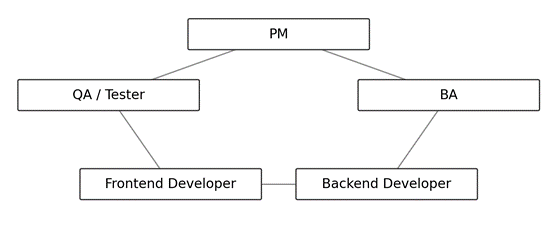
\includegraphics[width=0.82\textwidth]{Images/Picture1.png}
\caption{Cơ cấu phối hợp của nhóm dự án}
\label{fig:project-team-organization}
\end{figure}

Các đường nối trong Hình~\ref{fig:project-team-organization} minh họa quan hệ phối hợp giữa các vai trò, không thể hiện cấp bậc quản lý.

\tasksubheading{Vai trò và trách nhiệm}

\begin{itemize}
    \item \textbf{Quản lý dự án (Project Manager -- PM):} Chịu trách nhiệm lập kế hoạch, phân chia công việc và theo dõi tiến độ thực hiện trên Jira. PM phối hợp với các thành viên xác định mức độ ưu tiên của \textit{Backlog}, theo dõi những công việc bị chậm hoặc gặp trở ngại và điều chỉnh phân công phù hợp với năng lực của nhóm. Đồng thời, PM tổ chức hai buổi họp định kỳ mỗi tuần qua Google Meet, bảo đảm các vấn đề cần quyết định được đưa ra thảo luận và các kết luận quan trọng được cập nhật lên Confluence. Khi phát sinh yêu cầu mới, PM phối hợp với BA và đội ngũ kỹ thuật đánh giá tác động đến phạm vi, thời gian và nguồn lực trước khi thống nhất phương án xử lý. Bên cạnh công việc quản lý, PM tham gia thực hiện các phần việc Backend được phân công theo kế hoạch. Khi lập lịch, nhóm tính chung thời gian quản lý và thời gian lập trình của người PM để tránh phân công trùng thời điểm. Mã nguồn do PM tạo tuân thủ quy trình kiểm thử và Pull Request như các thành viên phát triển khác.

    \item \textbf{Phân tích nghiệp vụ (Business Analyst -- BA):} Chịu trách nhiệm tổng hợp, làm rõ và tài liệu hóa yêu cầu của hệ thống quản lý sự kiện. BA chuyển các yêu cầu đã thống nhất thành mô tả công việc hoặc \textit{User Story} có tiêu chí chấp nhận (\textit{Acceptance Criteria}) rõ ràng trên Jira, giúp lập trình viên và người kiểm thử hiểu thống nhất kết quả cần đạt. Các quy tắc nghiệp vụ như giới hạn số lượng đăng ký, thứ tự xử lý danh sách chờ, điều kiện chuyển sang danh sách chính thức và ghi nhận điểm danh được mô tả trên Confluence. BA cũng phối hợp với QA xây dựng các tình huống kiểm thử nghiệp vụ và đối chiếu sản phẩm với yêu cầu đã xác định. Ngoài phân tích nghiệp vụ và hỗ trợ kiểm thử, BA tham gia thiết kế mockups, lập trình giao diện tài khoản/phân quyền và giao diện báo cáo/tải tệp theo phân công. FE thống nhất cách kết nối API và review UI do BA thực hiện; QA kiểm thử các luồng hoàn chỉnh. BA vẫn giữ trách nhiệm làm rõ yêu cầu và tiêu chí chấp nhận.

    \item \textbf{Phát triển Backend (Backend Developer):} Chịu trách nhiệm đầu mối xây dựng phần xử lý phía máy chủ bằng Java Spring Boot, thiết kế cấu trúc dữ liệu và phát triển các API phục vụ ứng dụng. Backend Developer giữ đầu mối thống nhất thiết kế, API và tích hợp Backend; phụ trách tài khoản/phân quyền, giao dịch sức chứa/waitlist, xác thực QR và truy vấn báo cáo theo kế hoạch. BE thống nhất giao diện giữa các phần việc với PM và review Backend do PM thực hiện; PM nhận phần quản lý sự kiện, đăng ký/hủy, email, điểm danh thủ công và xuất tệp đã được xác định cụ thể. Backend Developer phối hợp với Frontend Developer để thống nhất cách trao đổi dữ liệu, cập nhật đặc tả API trên Confluence và xây dựng các kiểm thử đơn vị cho phần mã nguồn phụ trách. Mọi thay đổi được thực hiện trên nhánh riêng và gửi \textit{Pull Request} trên GitHub để thành viên khác kiểm duyệt trước khi sáp nhập.

    \item \textbf{Phát triển Frontend (Frontend Developer):} Chịu trách nhiệm đầu mối cấu trúc Angular, kết nối API và tích hợp giao diện; phụ trách các luồng sự kiện, đăng ký/waitlist và điểm danh. BA hỗ trợ các màn hình độc lập đã được phân công. FE thống nhất cách kết nối API và review mockups, mã UI do BA thực hiện cùng kết quả tích hợp trước khi chuyển kiểm thử. Thành viên phụ trách Frontend cũng thực hiện kiểm thử đơn vị phù hợp, cập nhật tiến độ trên Jira và tuân thủ quy trình \textit{Pull Request}, kiểm duyệt chéo trên GitHub.

    \item \textbf{Đảm bảo chất lượng và kiểm thử (Quality Assurance -- QA/Tester):} Chịu trách nhiệm lập các kịch bản kiểm thử dựa trên yêu cầu và tiêu chí chấp nhận đã thống nhất. Hoạt động kiểm thử tập trung vào tính đúng đắn của chức năng, sự phối hợp giữa giao diện và Backend, cũng như các luồng nghiệp vụ quan trọng như đăng ký, hủy đăng ký, tự động chuyển danh sách chờ và điểm danh bằng mã QR. QA ghi nhận lỗi trên Jira kèm các bước tái hiện, kết quả mong đợi và kết quả thực tế; sau khi lỗi được sửa, QA thực hiện kiểm thử lại và kiểm tra những chức năng liên quan. Vai trò này phối hợp với các thành viên đối chiếu điều kiện hoàn thành công việc theo \textit{Definition of Done} được quy định tại Mục~1.7.2.
\end{itemize}

\tasksubheading{Nguyên tắc kiêm nhiệm và kiểm tra chéo}

Nhóm thống nhất phân công 5 thành viên vào 5 vai trò chính như Bảng~\ref{tab:team-role-assignment}. Việc phân công một người phụ trách mỗi vai trò giúp xác định đầu mối chịu trách nhiệm rõ ràng; các nhiệm vụ hỗ trợ và kiểm tra chéo vẫn được thực hiện để duy trì khả năng phối hợp trong nhóm.

\begin{table}[H]
\centering
\renewcommand{\arraystretch}{1.2}
\begin{tabularx}{\textwidth}{|>{\centering\arraybackslash}p{2.2cm}|p{4.1cm}|X|}
\hline
\textbf{Thành viên} & \textbf{Vai trò chính} & \textbf{Nhiệm vụ phối hợp} \\
\hline
1 & PM & Kiêm hỗ trợ Backend theo tác vụ; vẫn điều phối, theo dõi và quản lý dự án \\
\hline
2 & BA & Hỗ trợ UI/Frontend: mockups, giao diện tài khoản/phân quyền, báo cáo; hỗ trợ kiểm thử nghiệp vụ \\
\hline
3 & Backend Developer & Đầu mối Backend; phối hợp và review phần PM thực hiện \\
\hline
4 & Frontend Developer & Đầu mối Frontend; phối hợp và review phần BA thực hiện \\
\hline
5 & QA/Tester & Phối hợp BA và Dev kiểm tra chất lượng \\
\hline
\end{tabularx}
\caption{Phân công vai trò chính và nhiệm vụ phối hợp}
\label{tab:team-role-assignment}
\end{table}

Bên cạnh trách nhiệm chính, các lập trình viên tham gia kiểm thử chéo và kiểm duyệt mã nguồn cho nhau trong phạm vi chuyên môn phù hợp. Người tạo \textit{Pull Request} không tự phê duyệt thay cho người kiểm duyệt độc lập; mã nguồn phải nhận được sự chấp thuận từ ít nhất một thành viên khác theo quy trình tại Mục~1.7.2. Việc lập trình viên tự kiểm thử phần việc của mình không thay thế hoạt động kiểm tra chéo hoặc kiểm thử tích hợp của nhóm.

Quy tắc kiểm duyệt độc lập áp dụng cả khi PM và BA kiêm lập trình: BE review Backend của PM; FE review mockups/UI của BA; QA review seed và kiểm thử độc lập. PM điều phối xử lý dựa trên kết quả kiểm tra. Người tạo không tự phê duyệt phần mình viết; vai trò quản lý hoặc phân tích nghiệp vụ không thay thế review kỹ thuật và kiểm thử.

Trách nhiệm ghi biên bản họp được luân phiên giữa các thành viên và xác định ở đầu mỗi buổi họp. Biên bản, quyết định và tài liệu nghiệp vụ được lưu trên Confluence; tiến độ và lỗi được theo dõi trên Jira; mã nguồn được quản lý trên GitHub. Zalo phục vụ trao đổi nhanh hằng ngày, còn Google Meet được sử dụng cho các buổi họp chính thức theo kế hoạch giao tiếp tại Mục~1.7.3.

\subsubsection{Relevant Standards and Procedures (Tiêu chuẩn và Quy trình dự án)}

Việc thiết lập các tiêu chuẩn và quy trình làm việc rõ ràng là nền tảng để bảo đảm tính nhất quán, minh bạch và chất lượng của sản phẩm phần mềm xuyên suốt vòng đời dự án. Nhóm áp dụng các quy trình quản lý và kỹ thuật sau:

\begin{itemize}
    \item \textbf{Quản lý dự án và tài liệu (Project and Documentation Management):} Dự án sử dụng hệ sinh thái Atlassian để quản lý tiến độ và tri thức. Jira Software được sử dụng làm công cụ cốt lõi để theo dõi vòng đời của từng tác vụ (\textit{Issue Tracking}), quản lý danh sách công việc (\textit{Backlog}) và phân công nguồn lực. Song song đó, Confluence, với phiên bản miễn phí hỗ trợ nhóm dưới 10 người, đóng vai trò là không gian lưu trữ tài liệu tập trung (\textit{Single Source of Truth}), nơi nhóm biên soạn và lưu trữ biên bản họp (\textit{Meeting Minutes}), đặc tả API và tài liệu kiến trúc hệ thống.

    \item \textbf{Quy trình quản lý mã nguồn (Version Control System):} Toàn bộ mã nguồn của dự án được lưu trữ và quản lý phiên bản tập trung trên GitHub. Nhóm áp dụng chiến lược phân nhánh \textit{Feature Branch Workflow} để bảo đảm tính ổn định của mã nguồn chính. Mọi tính năng mới hoặc bản vá lỗi phải được phát triển trên một nhánh riêng biệt (\textit{feature branch}) tách ra từ nhánh phát triển gốc. Mã nguồn chỉ được sáp nhập (\textit{merge}) thông qua \textit{Pull Request} sau khi hoàn thành các bước kiểm duyệt kỹ thuật.

    \item \textbf{Tiêu chuẩn công nghệ và lập trình (Coding Standards):} Dự án định hướng sử dụng Java Spring Boot cho hệ thống Backend nhằm hỗ trợ xử lý nghiệp vụ và bảo mật, kết hợp Angular cho nền tảng Frontend để xây dựng giao diện tương tác. Thành viên phải tuân thủ các quy chuẩn viết mã (\textit{Coding Conventions}) của từng ngôn ngữ, bao gồm quy tắc đặt tên biến/hàm, cấu trúc thư mục và các nguyên tắc \textit{Clean Code} nhằm nâng cao khả năng đọc hiểu và bảo trì mã nguồn.

    \item \textbf{Tiêu chuẩn nghiệm thu (Definition of Done -- DoD):} Một tác vụ lập trình chỉ được xem là hoàn thành (\textit{Done}) khi đáp ứng đầy đủ các điều kiện sau:
    \begin{itemize}
        \item mã nguồn biên dịch thành công và ứng dụng vận hành không phát sinh lỗi thực thi (\textit{runtime error}) trên môi trường phát triển;
        \item vượt qua các kịch bản kiểm thử đơn vị (\textit{Unit Test}) cơ bản;
        \item mã nguồn đã được đẩy (\textit{push}) lên GitHub và tạo \textit{Pull Request} hợp lệ;
        \item vượt qua quy trình kiểm duyệt chéo (\textit{Peer Code Review}) và nhận được sự chấp thuận (\textit{Approve}) từ ít nhất một thành viên khác trong nhóm.
    \end{itemize}
\end{itemize}

\begin{figure}[H]
\centering
\begin{tabularx}{\textwidth}{>{\centering\arraybackslash}X >{\centering\arraybackslash}X}
    
\includegraphics[height=2.4cm,keepaspectratio]{Images/Picture2.png} &
    
\includegraphics[height=2.4cm,keepaspectratio]{Images/Picture3.png} \\
    \textbf{Jira Software} & \textbf{Confluence}
\end{tabularx}
\vspace{0.3cm}
\caption{Các công cụ quản lý dự án và tài liệu được nhóm sử dụng}
\label{fig:project-management-tools}
\end{figure}

\subsubsection{Communication Methods (Phương thức giao tiếp)}

Để duy trì sự đồng bộ thông tin và bảo đảm khả năng phản ứng trước các rủi ro hoặc thay đổi yêu cầu, nhóm thiết lập kế hoạch giao tiếp (\textit{Communication Plan}) kết hợp giữa các kênh trao đổi tức thời và các buổi họp định kỳ.

\begin{itemize}
    \item \textbf{Kênh trao đổi hằng ngày (Daily Communication):} Nhóm sử dụng Zalo làm kênh giao tiếp nội bộ cho các hoạt động trao đổi tức thời. Kênh này được sử dụng để thông báo các cập nhật nhanh, trao đổi về các trở ngại kỹ thuật (\textit{blocker}) phát sinh trong quá trình phát triển và nhắc nhở tiến độ của các tác vụ trên Jira.

    \item \textbf{Kênh họp trực tuyến (Virtual Meetings):} Các cuộc họp chính thức nhằm báo cáo tiến độ, lập kế hoạch (\textit{Planning}) hoặc thảo luận giải pháp kỹ thuật được tổ chức qua Google Meet và sử dụng chức năng chia sẻ màn hình khi cần thiết.

    \item \textbf{Tần suất và nội dung cuộc họp (Meeting Cadence):} Nhóm duy trì hai buổi họp định kỳ mỗi tuần, mỗi buổi kéo dài trung bình 30 phút. Nội dung họp tập trung vào ba vấn đề: (1) báo cáo những công việc đã hoàn thành; (2) nhận diện và tháo gỡ các khó khăn hiện tại; và (3) thống nhất danh sách công việc của increment hiện tại hoặc tiếp theo. Các quyết định quan trọng được người ghi biên bản của buổi họp tổng hợp và cập nhật lên Confluence.

Sau khi Increment 1 hoàn thành kiểm thử, nhóm dự kiến sử dụng một buổi họp định kỳ để trình diễn bản thử nghiệm cho thầy Nguyễn Minh Tâm, với vai trò đại diện khách hàng, tại checkpoint CP1. PM thống nhất lịch demo, BA tổng hợp câu hỏi nghiệp vụ và cùng PM ghi nhận phản hồi vào Client Interaction Log. Nhóm gửi liên kết bản demo, phiên bản/build và các nội dung cần xác nhận qua Gmail; trao đổi trực tiếp có thể thực hiện qua Google Meet theo lịch đã thống nhất. Các phản hồi được đánh giá tác động trước khi điều chỉnh sản phẩm.
\end{itemize}

\begin{table}[H]
\centering
\renewcommand{\arraystretch}{1.2}
\begin{tabularx}{\textwidth}{|p{2.5cm}|p{3cm}|X|p{2.7cm}|}
\hline
\textbf{Kênh} & \textbf{Tần suất} & \textbf{Mục đích sử dụng} & \textbf{Nơi ghi nhận} \\
\hline
Zalo & Hằng ngày/khi cần & Cập nhật nhanh, trao đổi trở ngại và nhắc tiến độ & Jira hoặc Confluence nếu cần truy vết \\
\hline
Google Meet & 2 buổi/tuần, khoảng 30 phút/buổi & Báo cáo tiến độ, lập kế hoạch và thảo luận vấn đề cần quyết định & Biên bản trên Confluence \\
\hline
Gmail; Google Meet khi đã thống nhất lịch & Tại CP1 sau kiểm thử I1 và khi cần xác nhận yêu cầu/thay đổi & Gửi bản demo và câu hỏi cần xác nhận; tiếp nhận phản hồi, làm rõ tác động và quyết định & Client Interaction Log trên Confluence; liên kết email/biên bản tương ứng \\
\hline
Jira & Cập nhật theo tác vụ & Quản lý \textit{Backlog}, phân công, tiến độ và lỗi & Jira \\
\hline
Confluence & Cập nhật sau họp hoặc khi tài liệu thay đổi & Lưu biên bản, quyết định, yêu cầu, đặc tả API và kiến trúc & Confluence \\
\hline
GitHub & Theo hoạt động phát triển & Quản lý mã nguồn, \textit{Pull Request} và kiểm duyệt chéo & GitHub \\
\hline
\end{tabularx}
\caption{Kế hoạch giao tiếp của nhóm dự án}
\label{tab:communication-plan}
\end{table}
\subsection{Analyze project characteristics, determine whether the project is primarily objective-based or product-based, identify high-level project risks, and select a suitable general development lifecycle/approach with justification.}

\subsubsection{Phân tích đặc điểm dự án}

Các đặc điểm chính của dự án và ảnh hưởng của chúng đến công tác lập kế hoạch được tổng hợp trong Bảng~\ref{tab:project-characteristics}.

{%
\setlength{\tabcolsep}{4pt}
\renewcommand{\arraystretch}{1.2}
\begin{longtable}{|p{3.1cm}|p{6.1cm}|p{5.5cm}|}
\caption{Phân tích đặc điểm của dự án}\label{tab:project-characteristics}\\
\hline
\textbf{Đặc điểm dự án} & \textbf{Phân tích đối với dự án} & \textbf{Ý nghĩa đối với việc lập kế hoạch} \\
\hline
\endfirsthead
\multicolumn{3}{c}{\textit{Bảng~\thetable{} (tiếp theo)}}\\
\hline
\textbf{Đặc điểm dự án} & \textbf{Phân tích đối với dự án} & \textbf{Ý nghĩa đối với việc lập kế hoạch} \\
\hline
\endhead
\hline
\multicolumn{3}{r}{\textit{Còn tiếp ở trang sau}}\\
\endfoot
\hline
\endlastfoot
\textbf{Quy mô và nguồn lực} & Dự án có quy mô nhỏ, do nhóm \textbf{5 thành viên} thực hiện trong thời gian bài tập lớn. Sản phẩm cần đủ hoàn chỉnh để triển khai, kiểm thử và trình diễn; phạm vi phải phù hợp với thời gian và năng lực của nhóm. & Ưu tiên các luồng nghiệp vụ cốt lõi của MVP; chức năng có mức ưu tiên thấp chỉ được thực hiện khi còn đủ thời gian và nguồn lực. \\
\hline
\textbf{Loại hệ thống} & Đây là hệ thống thông tin (\textit{information system}) phục vụ quản lý thông tin sự kiện, đăng ký/hủy đăng ký, sức chứa, danh sách chờ, điểm danh và báo cáo. Mã QR là phương thức hỗ trợ điểm danh; phạm vi hiện tại không yêu cầu phần cứng chuyên dụng hoặc xử lý thời gian thực đặc thù của hệ thống nhúng. & Tập trung vào yêu cầu nghiệp vụ, dữ liệu, phân quyền, tính chính xác của trạng thái và kiểm thử các luồng sử dụng. \\
\hline
\textbf{Phạm vi nghiệp vụ} & MVP đã được xác định tương đối rõ: tạo, quản lý và công bố sự kiện; đăng ký/hủy; quản lý sức chứa và danh sách chờ; điểm danh bằng mã QR hoặc thủ công; gửi email; báo cáo cơ bản; và quản lý tài khoản, quyền truy cập. SMS, hệ thống gợi ý, phân tích nâng cao, tích hợp MyBK và đồng bộ ngoại tuyến đầy đủ không thuộc phạm vi cốt lõi. & Có thể xác định các sản phẩm cần bàn giao và phân rã thành các thành phần nhỏ hơn để lập kế hoạch. \\
\hline
\textbf{Mức độ rõ của yêu cầu} & Các yêu cầu chức năng và quy tắc chính đã được làm rõ để xác định MVP. Tuy nhiên, số sự kiện thực tế, quy mô người dùng, thời gian xử lý hiện tại và mức cải thiện kỳ vọng chưa có số liệu thực tế được xác nhận. & Có thể lập \textit{baseline} cho phạm vi chức năng. Những giá trị chưa được xác nhận cần ghi nhận dưới dạng giả định và cập nhật khi có dữ liệu đáng tin cậy. \\
\hline
\textbf{Bên liên quan và mức độ chấp nhận} & Sinh viên quan tâm đến trải nghiệm đăng ký và trạng thái tham gia; người tổ chức quan tâm đến sự kiện, người tham dự, điểm danh và báo cáo; quản trị viên quan tâm đến tài khoản và phân quyền. Đại diện khách hàng xác nhận yêu cầu và các quyết định quan trọng. & Duy trì trao đổi với các bên liên quan chính, đặc biệt là khách hàng và người tổ chức; kiểm thử các luồng quan trọng với người dùng đại diện khi có thể. \\
\hline
\textbf{Công nghệ và tích hợp} & Khách hàng không áp đặt nền tảng Web/Mobile hoặc công nghệ cụ thể. Dữ liệu sinh viên có thể được giả lập; MVP không yêu cầu kết nối MyBK hoặc cơ sở dữ liệu thật của trường. Các phụ thuộc bên ngoài chủ yếu gồm môi trường triển khai và dịch vụ email. & Chọn công nghệ phù hợp với năng lực nhóm và thời gian thực hiện; tránh các tích hợp không cần thiết làm tăng độ phức tạp. \\
\hline
\textbf{Yêu cầu chất lượng} & Hệ thống phải bảo vệ thông tin cá nhân, kiểm soát truy cập theo vai trò và duy trì tính nhất quán của dữ liệu đăng ký, sức chứa, danh sách chờ và điểm danh. Hệ thống cần ngăn đăng ký trùng và hiển thị sai trạng thái; đồng thời có phương án điểm danh thủ công khi mã QR hoặc mạng gặp sự cố. & Chuyển yêu cầu chất lượng thành tiêu chí chấp nhận và ca kiểm thử. Kiểm tra cả luồng chính và luồng dự phòng; làm rõ cách ghi nhận tạm thời khi mất mạng và cập nhật sau đó. \\
\hline
\textbf{Ràng buộc tiến độ} & Dự án tuân theo các mốc của học phần và cần có bằng chứng quản lý trong quá trình thực hiện. Việc mở rộng phạm vi quá mức có thể ảnh hưởng đến khả năng hoàn thành và kiểm thử sản phẩm. & Lập \textit{baseline} phạm vi và tiến độ rõ ràng, theo dõi tiến độ thực tế và kiểm soát thay đổi để bảo vệ các chức năng cốt lõi. \\
\hline
\end{longtable}
}

\subsubsection{Xác định định hướng objective-based hoặc product-based}

Cách tiếp cận \textit{objective-based} bắt đầu từ các mục tiêu cần đạt và có thể xem xét nhiều phương án khác nhau để đạt các mục tiêu đó. Ngược lại, cách tiếp cận \textit{product-based} bắt đầu từ sản phẩm cần tạo ra và các đặc tính chính đã được xác định. Bảng~\ref{tab:objective-product-analysis} phân tích định hướng phù hợp với dự án.

{%
\setlength{\tabcolsep}{4pt}
\renewcommand{\arraystretch}{1.2}
\begin{longtable}{|p{3.5cm}|p{8.5cm}|p{2.7cm}|}
\caption{Phân tích định hướng objective-based và product-based}\label{tab:objective-product-analysis}\\
\hline
\textbf{Khía cạnh} & \textbf{Phân tích} & \textbf{Khuynh hướng} \\
\hline
\endfirsthead
\multicolumn{3}{c}{\textit{Bảng~\thetable{} (tiếp theo)}}\\
\hline
\textbf{Khía cạnh} & \textbf{Phân tích} & \textbf{Khuynh hướng} \\
\hline
\endhead
\hline
\endfoot
\hline
\endlastfoot
\textbf{Mục tiêu nghiệp vụ} & Dự án hướng đến giảm sự phân tán dữ liệu, giảm thao tác thủ công khi quản lý đăng ký và điểm danh, rút ngắn thời gian tổng hợp và cải thiện tính nhất quán dữ liệu. Đây là các kết quả nghiệp vụ cần đạt. & Thể hiện mục tiêu nghiệp vụ của dự án. \\
\hline
\textbf{Sản phẩm cần bàn giao} & Giải pháp đã được xác định là một hệ thống phần mềm tập trung hỗ trợ tổ chức và quản lý sự kiện. Nhóm không phải lựa chọn giữa nhiều loại giải pháp hoàn toàn khác nhau. & \textit{Product-based} \\
\hline
\textbf{Phạm vi chức năng} & Các chức năng cốt lõi và giới hạn MVP đã được làm rõ tương đối cụ thể qua \textit{Client Interaction Log}. & \textit{Product-based} \\
\hline
\textbf{Mức độ tự do về cách thực hiện} & Nhóm được tự chọn nền tảng và công nghệ nhưng vẫn phải xây dựng hệ thống với các chức năng đã thống nhất. Sự linh hoạt về kỹ thuật không làm thay đổi sản phẩm cần bàn giao. & Phù hợp với \textit{product-based} \\
\hline
\textbf{Nghiệm thu và bàn giao} & Nhóm phải bàn giao hệ thống vận hành được, có thể kiểm thử và trình diễn các chức năng thuộc phạm vi đã thống nhất. & \textit{Product-based} \\
\hline
\end{longtable}
}

\textbf{Dự án chủ yếu theo định hướng product-based}, vì sản phẩm cần bàn giao đã được xác định và phạm vi MVP tương đối rõ. Nhóm có thể bắt đầu lập kế hoạch từ các sản phẩm cần tạo ra, phân rã thành sản phẩm con, sau đó xác định các hoạt động xây dựng, tích hợp và kiểm thử.

Dự án vẫn có các mục tiêu nghiệp vụ cần được đánh giá riêng. Việc hoàn thành đầy đủ chức năng chưa tự động chứng minh rằng hệ thống đã giảm thao tác thủ công, rút ngắn thời gian tổng hợp hoặc cải thiện tính nhất quán dữ liệu. Vì vậy, các sản phẩm bàn giao được dùng để kiểm soát việc hoàn thành sản phẩm, còn mục tiêu nghiệp vụ được đánh giá bằng các thước đo hiệu quả phù hợp.

Từ kết quả phân tích, nhóm định hướng lập kế hoạch như sau:
\begin{itemize}
    \item sử dụng \textit{Product Breakdown Structure (PBS)} để xác định và phân rã sản phẩm cần bàn giao;
    \item xây dựng \textit{Product Descriptions} cho các sản phẩm quan trọng để làm rõ nội dung, tiêu chí chất lượng và điều kiện hoàn thành;
    \item sử dụng \textit{Product Flow Diagram (PFD)} để thể hiện quan hệ giữa các sản phẩm, sau đó xác định các hoạt động cần thiết;
    \item gắn \textit{baseline} với phạm vi đã thống nhất và kiểm soát các thay đổi ảnh hưởng đến sản phẩm bàn giao;
    \item ghi rõ giả định đối với thông tin chưa được xác nhận và cập nhật khi có dữ liệu đáng tin cậy.
\end{itemize}

\subsubsection{Rủi ro dự án ở mức tổng quát}

Nhóm đánh giá khả năng xảy ra (\textit{likelihood}) và mức độ ảnh hưởng (\textit{impact}) theo ba mức: Cao, Trung bình và Thấp. Đây là đánh giá sơ bộ dựa trên yêu cầu và điều kiện thực hiện dự án.

{%
\setlength{\tabcolsep}{3pt}
\renewcommand{\arraystretch}{1.2}
\begin{longtable}{|p{0.7cm}|p{5.1cm}|p{1.7cm}|p{1.5cm}|p{5.4cm}|}
\caption{Các rủi ro dự án ở mức tổng quát}\label{tab:high-level-risks}\\
\hline
\textbf{ID} & \textbf{Rủi ro dự án} & \textbf{Khả năng} & \textbf{Ảnh hưởng} & \textbf{Hướng xử lý sơ bộ} \\
\hline
\endfirsthead
\multicolumn{5}{c}{\textit{Bảng~\thetable{} (tiếp theo)}}\\
\hline
\textbf{ID} & \textbf{Rủi ro dự án} & \textbf{Khả năng} & \textbf{Ảnh hưởng} & \textbf{Hướng xử lý sơ bộ} \\
\hline
\endhead
\hline
\multicolumn{5}{r}{\textit{Còn tiếp ở trang sau}}\\
\endfoot
\hline
\endlastfoot
R1 & \textbf{Phạm vi mở rộng quá mức.} Việc bổ sung bảng điều khiển theo học kỳ, chức năng nâng cao hoặc tích hợp mới có thể khiến khối lượng công việc vượt khả năng của nhóm. & Trung bình & Cao & Chốt phạm vi MVP, ưu tiên chức năng cốt lõi và đánh giá công sức, tiến độ trước khi trình khách hàng xác nhận phần bổ sung. \\
\hline
R2 & \textbf{Ước lượng thiếu công sức dẫn đến trễ tiến độ.} Danh sách chờ, phân quyền, điểm danh và email có nhiều tình huống cần xử lý và kiểm thử. & Trung bình & Cao & Chia nhỏ công việc, tính cả công sức kiểm thử, theo dõi tiến độ thường xuyên và dành thời gian dự phòng. \\
\hline
R3 & \textbf{Thiếu dữ liệu để xác định yêu cầu và đánh giá hiệu quả.} Chưa có thông tin định lượng đầy đủ về quy mô sử dụng và quy trình hiện tại nên nhóm có thể đặt yêu cầu hoặc mục tiêu chưa phù hợp. & Cao & Trung bình & Ghi rõ giả định và mục tiêu đề xuất, tiếp tục làm rõ thông tin quan trọng với khách hàng và nêu giới hạn khi đánh giá bằng dữ liệu thử nghiệm. \\
\hline
R4 & \textbf{Sai lệch dữ liệu nghiệp vụ.} Lỗi xử lý có thể gây đăng ký trùng, vượt sức chứa, chuyển danh sách chờ sai hoặc tạo báo cáo không chính xác. & Trung bình & Cao & Xác định quy tắc cập nhật trạng thái; kiểm thử đăng ký đồng thời, hủy và chuyển danh sách chờ; đối chiếu báo cáo với dữ liệu đã biết kết quả. \\
\hline
R5 & \textbf{Lỗi phân quyền hoặc lộ thông tin cá nhân.} Người dùng có thể truy cập dữ liệu hoặc thực hiện thao tác ngoài quyền được cấp. & Trung bình & Cao & Xác định quyền của từng vai trò, kiểm tra quyền ở phía hệ thống, kiểm thử truy cập trái quyền và sử dụng dữ liệu sinh viên giả lập. \\
\hline
R6 & \textbf{Sự cố kỹ thuật làm gián đoạn hệ thống.} Mã QR, mạng, môi trường triển khai hoặc dịch vụ email gặp lỗi có thể ảnh hưởng đến điểm danh và thông báo. & Trung bình & Cao & Kiểm tra sớm môi trường triển khai và email; chuẩn bị cách điểm danh thủ công, làm rõ cách ghi nhận tạm thời khi mất mạng và cập nhật sau; theo dõi lỗi gửi thông báo. \\
\hline
R7 & \textbf{Nguồn lực nhóm không đáp ứng kế hoạch.} Lịch học, công việc khác hoặc kỹ năng của thành viên có thể làm giảm thời gian thực hiện so với dự kiến. & Trung bình & Cao & Lập kế hoạch theo thời gian tham gia thực tế, phân công phù hợp với năng lực và chia sẻ tài liệu, mã nguồn để các thành viên có thể hỗ trợ nhau. \\
\hline
\end{longtable}
}

\subsubsection{Lựa chọn vòng đời và cách tiếp cận phát triển}

\tasksubheading{Cơ sở lựa chọn}

Việc lựa chọn vòng đời phát triển cần phù hợp với đặc điểm dự án và các rủi ro đã xác định. Hệ thống đăng ký và quản lý sự kiện có phạm vi MVP tương đối rõ, nhưng một số nội dung như cách xử lý tình huống ngoại lệ, giao diện sử dụng và tiêu chí kiểm chứng chi tiết vẫn cần được hoàn thiện trong quá trình triển khai. Các chức năng cũng có quan hệ phụ thuộc: đăng ký cần thông tin sự kiện và sức chứa; danh sách chờ phụ thuộc vào đăng ký và hủy; báo cáo sử dụng dữ liệu đăng ký và điểm danh. Vì vậy, nhóm cần tổ chức phát triển theo trình tự phù hợp, đồng thời kiểm tra tính nhất quán khi bổ sung từng phần.

Dự án được thực hiện bởi năm thành viên trong thời gian giới hạn của học phần. Phương pháp phát triển cần giúp nhóm kiểm chứng các luồng nghiệp vụ sớm, theo dõi tiến độ bằng kết quả có thể trình diễn và tiếp nhận phản hồi trước khi hoàn thiện toàn bộ sản phẩm. Việc lựa chọn cũng phải hỗ trợ quản lý \textit{baseline}, ghi nhận công sức thực tế và kiểm soát những thay đổi ảnh hưởng đến phạm vi đã thống nhất.

\tasksubheading{So sánh các cách tiếp cận}

\begin{table}[H]
\centering
\renewcommand{\arraystretch}{1.2}
\begin{tabularx}{\textwidth}{|p{3.3cm}|X|X|}
\hline
\textbf{Cách tiếp cận} & \textbf{Điểm phù hợp với dự án} & \textbf{Hạn chế cần xem xét} \\
\hline
\textbf{Waterfall} & Các giai đoạn và sản phẩm trung gian rõ ràng; phù hợp với những yêu cầu đã được xác định và thuận tiện bố trí các điểm kiểm tra. & Nếu chỉ kiểm chứng sản phẩm hoàn chỉnh ở cuối quá trình, nhóm có thể phát hiện muộn sai lệch về nghiệp vụ hoặc giao diện. Việc sửa đổi khi đó có thể ảnh hưởng đến nhiều thành phần. \\
\hline
\textbf{Evolutionary Prototyping} & Cho phép làm rõ yêu cầu qua sản phẩm thử nghiệm và phản hồi của người dùng; hữu ích đối với các luồng tương tác chưa được thống nhất. & Nếu liên tục mở rộng nguyên mẫu mà thiếu thiết kế và kiểm soát phạm vi, nhóm có thể phát sinh công sức sửa lại hoặc khó duy trì chất lượng sản phẩm. \\
\hline
\textbf{Incremental Development} & Chia MVP thành các phần có thể xây dựng, tích hợp và kiểm chứng lần lượt; giúp theo dõi tiến độ và phát hiện vấn đề trước khi hoàn thành toàn bộ hệ thống. & Cần xác định kiến trúc, dữ liệu dùng chung và quan hệ phụ thuộc giữa các phần từ đầu; phải kiểm thử lại các chức năng liên quan sau mỗi lần tích hợp. \\
\hline
\end{tabularx}
\caption{So sánh các cách tiếp cận phát triển}
\label{tab:development-approach-comparison}
\end{table}

\tasksubheading{Vòng đời phát triển được lựa chọn}

Nhóm lựa chọn \textbf{phát triển gia tăng (\textit{Incremental Development}), kết hợp các vòng lặp hoàn thiện trong từng phần phát triển}. Phạm vi MVP được xác định ở mức tổng thể trước khi triển khai, sau đó được chia thành các phần chức năng theo quan hệ phụ thuộc và mức độ ưu tiên. Mỗi phần trải qua các hoạt động làm rõ yêu cầu chi tiết, thiết kế, lập trình, kiểm thử và đánh giá trước khi tích hợp vào hệ thống chung.

Sau mỗi phần phát triển, nhóm rà soát kết quả và tiếp nhận phản hồi để sửa lỗi hoặc hoàn thiện những nội dung thuộc phạm vi đã thống nhất. Khi còn điểm chưa rõ về giao diện hoặc cách thao tác, nhóm có thể sử dụng nguyên mẫu đơn giản để trao đổi trước khi lập trình đầy đủ. Nguyên mẫu đóng vai trò hỗ trợ làm rõ yêu cầu; kết quả bàn giao vẫn phải đáp ứng các tiêu chí chất lượng và kiểm thử của sản phẩm chính thức.

Các phiên bản gia tăng trước hết được sử dụng để kiểm thử và trình diễn trong phạm vi nhóm và khách hàng. Việc đưa một phiên bản vào vận hành thực tế chỉ được thực hiện khi có sự thống nhất về phạm vi, chất lượng và điều kiện sử dụng.

\tasksubheading{Định hướng tổ chức phát triển}

Trước khi xây dựng các phần chức năng, nhóm thống nhất cấu trúc dữ liệu, phân quyền, quy tắc chuyển trạng thái và cách tích hợp giữa các thành phần. Những nội dung dùng chung này tạo cơ sở để các thành viên làm việc nhất quán và hạn chế sửa đổi khi tích hợp.

\begin{table}[H]
\centering
\renewcommand{\arraystretch}{1.2}
\begin{tabularx}{\textwidth}{|p{3.6cm}|X|X|}
\hline
\textbf{Phần phát triển} & \textbf{Nội dung chính} & \textbf{Kết quả cần kiểm chứng} \\
\hline
\textbf{Phần 1: Quản lý và công bố sự kiện} & Tài khoản và phân quyền cơ bản; tạo, cập nhật và công bố sự kiện; sinh viên xem thông tin. & Người tổ chức quản lý sự kiện trong phạm vi quyền hạn; sinh viên xem được thông tin sự kiện đã công bố. \\
\hline
\textbf{Phần 2: Đăng ký và quản lý người tham gia} & Đăng ký/hủy; kiểm soát sức chứa và điều kiện tham gia; ngăn đăng ký trùng; danh sách chờ và các email quan trọng. & Luồng đăng ký hoạt động nhất quán; khi có chỗ trống, người đầu tiên trong danh sách chờ được chuyển sang danh sách chính thức và hệ thống thực hiện gửi thông báo. \\
\hline
\textbf{Phần 3: Điểm danh và báo cáo} & Điểm danh bằng mã QR và thủ công; chỉnh sửa kết quả điểm danh theo quyền; báo cáo cơ bản và xuất Excel/CSV. & Kết quả tham dự được ghi nhận chính xác; báo cáo và dữ liệu xuất khớp với các bản ghi đã được kiểm chứng. \\
\hline
\end{tabularx}
\caption{Định hướng các phần phát triển gia tăng}
\label{tab:development-increments}
\end{table}

Bản Increment 1 đã kiểm thử được sử dụng làm bản thử nghiệm để trình diễn và lấy phản hồi từ đại diện khách hàng tại CP1. Nhóm ghi nhận các nhận xét về giao diện, luồng thao tác và mức độ đáp ứng yêu cầu. Lỗi thuộc phạm vi đã thống nhất được sửa và kiểm thử lại trong hoạt động tương ứng. Phản hồi làm thay đổi phạm vi, tiêu chí nghiệm thu hoặc baseline phải được phân tích tác động và trình duyệt theo cơ chế tại Mục~1.5 trước khi thực hiện. Các increment tiếp theo kế thừa phiên bản đã được kiểm chứng và các điều chỉnh được chấp thuận.

Sau mỗi lần tích hợp, nhóm kiểm thử lại các chức năng liên quan để phát hiện ảnh hưởng của phần mới đối với phần đã hoàn thành. Trước khi bàn giao, nhóm kiểm thử toàn bộ quy trình từ công bố sự kiện, đăng ký và xử lý danh sách chờ đến điểm danh và xuất báo cáo. Thời lượng, nhân sự và mốc hoàn thành của từng phần được xác định trong kế hoạch chi tiết tại Task 2.

\tasksubheading{Giải thích sự phù hợp của phương pháp}

\textbf{Phù hợp với tính chất product-based và phạm vi MVP.} Sản phẩm cần bàn giao đã được xác định tương đối rõ, nên nhóm có thể phân chia hệ thống thành các phần chức năng cụ thể và xác lập điều kiện hoàn thành cho từng phần. Cách tổ chức này hỗ trợ lập kế hoạch từ sản phẩm, xác định hoạt động cần thực hiện và kiểm tra tiến độ thông qua kết quả đã xây dựng. Các phần phát triển vẫn hướng đến cùng một hệ thống thống nhất, bảo đảm quy trình cuối cùng hoạt động xuyên suốt.

\textbf{Hỗ trợ xử lý những yêu cầu cần tiếp tục làm rõ.} Mặc dù các quy tắc chính đã được xác nhận, giao diện và tình huống ngoại lệ cần được kiểm chứng khi có sản phẩm vận hành được. Việc trình diễn từng phần giúp nhóm trao đổi cụ thể với khách hàng, phát hiện cách hiểu chưa thống nhất và điều chỉnh trước khi các chức năng phụ thuộc được triển khai đầy đủ. Điều này góp phần xử lý rủi ro R3 về thông tin chưa đầy đủ, nhưng các giả định về quy mô sử dụng và hiệu quả vẫn phải được kiểm chứng riêng.

\textbf{Giảm nguy cơ phát hiện muộn lỗi nghiệp vụ và tích hợp.} Đăng ký, sức chứa, danh sách chờ và điểm danh có nhiều trạng thái liên quan. Phát triển từng phần cho phép nhóm kiểm tra các quy tắc này ngay khi chức năng tương ứng được hoàn thành, sau đó kiểm thử lại khi tích hợp. Môi trường triển khai và dịch vụ email cũng cần được thử nghiệm sớm thay vì chờ đến giai đoạn bàn giao. Cách thực hiện này hỗ trợ kiểm soát các rủi ro R4, R5 và R6 về dữ liệu, phân quyền và sự cố kỹ thuật.

\textbf{Phù hợp với nguồn lực và tiến độ giới hạn.} Mỗi phần phát triển có kết quả và điểm kiểm tra rõ ràng, giúp Project Manager so sánh tiến độ thực tế với kế hoạch và nhận biết sớm những công việc chậm hoặc cần hỗ trợ. Nhóm có thể ưu tiên hoàn thành các chức năng cốt lõi trước khi xem xét nội dung có mức ưu tiên thấp. Nếu xuất hiện nguy cơ vượt nguồn lực hoặc trễ tiến độ, nhóm có cơ sở phân tích phương án điều chỉnh và trình khách hàng xem xét, hỗ trợ kiểm soát các rủi ro R1, R2 và R7.

\textbf{Duy trì kiểm soát kế hoạch và thay đổi.} Phát triển gia tăng được kết hợp với lập kế hoạch theo \textit{Step Wise}. Nhóm vẫn thiết lập \textit{Project Baseline V1.0}, xác định sản phẩm, hoạt động, công sức, nguồn lực, rủi ro và các điểm kiểm tra. Nguyễn Đăng Khoa điều phối việc thực hiện và cập nhật kế hoạch chi tiết trong phạm vi được giao. Phản hồi làm thay đổi yêu cầu đã cam kết, tiêu chí nghiệm thu hoặc mốc bàn giao phải được phân tích tác động và trình thầy Nguyễn Minh Tâm xem xét theo cơ chế tại Mục~1.5. Các phiên bản \textit{baseline} được lưu giữ để đối chiếu với kết quả thực tế.

\section{Task 2: Product-Based Planning}

\subsection{Identify products and construct the PBS}
\subsubsection{Xác định và phân nhóm sản phẩm (Identify products)}
Dựa trên yêu cầu xây dựng MVP của Hệ thống đăng ký và quản lý sự kiện cũng như định hướng phát triển product-based đã được xác định ở Task 1.8, nhóm tiến hành phân rã dự án thành các sản phẩm cụ thể. Việc xác định sản phẩm không chỉ tập trung vào mã nguồn phần mềm mà phải bao quát toàn bộ vòng đời dự án nhằm cung cấp minh chứng cho các quyết định quản lý theo đúng yêu cầu của học phần.

Cấu trúc sản phẩm (PBS) bao gồm cả sản phẩm phần mềm và hồ sơ quản lý, được phân rã thành ba nhóm chính:

Sản phẩm Quản lý dự án (Management Products): Bao gồm các tài liệu thiết lập đường cơ sở (Project Baseline), hồ sơ theo dõi tiến độ hàng tuần (Weekly logs), phân tích rủi ro và các báo cáo tổng kết dự án. Đây là nhóm sản phẩm nòng cốt để minh chứng cho việc nhóm đã lập kế hoạch, giám sát và kiểm soát dự án một cách có kỷ luật.

Sản phẩm Kỹ thuật \& Phần mềm (Technical \& Software Products): Bao gồm các tài liệu thiết kế hệ thống (lược đồ CSDL, đặc tả API), các thành phần mã nguồn (Frontend, Backend) và cấu hình môi trường triển khai. Nhóm sản phẩm này cấu thành nên phiên bản MVP hoàn chỉnh hỗ trợ quy trình từ tạo sự kiện, đăng ký, điểm danh đến xuất báo cáo.

Sản phẩm Chất lượng (Quality Products): Bao gồm các kịch bản kiểm thử (Test cases/Acceptance criteria), bộ dữ liệu sinh viên giả lập và các minh chứng nghiệm thu chất lượng (Quality evidence). Nhóm sản phẩm này đảm bảo hệ thống đáp ứng các yêu cầu về phân quyền, tính nhất quán dữ liệu và xử lý mượt mà các luồng nghiệp vụ quan trọng.

Lưu ý rằng, căn cứ vào phần giới hạn phạm vi dự án (Exclusions), các thành phần liên quan đến hệ thống gợi ý (Recommendation), gửi tin nhắn SMS, tích hợp cơ sở dữ liệu MyBK hay xuất báo cáo PDF sẽ không được đưa vào cấu trúc sản phẩm phân rã này nhằm bảo vệ nguồn lực và tiến độ dự án.

\newgeometry{margin=1cm,includefoot}
\begin{landscape}
\landscapeheader
\subsubsection{Sơ đồ PBS}
\begin{figure}[H]
\centering
\begin{adjustbox}{max width=.98\linewidth,max totalheight=.78\textheight}
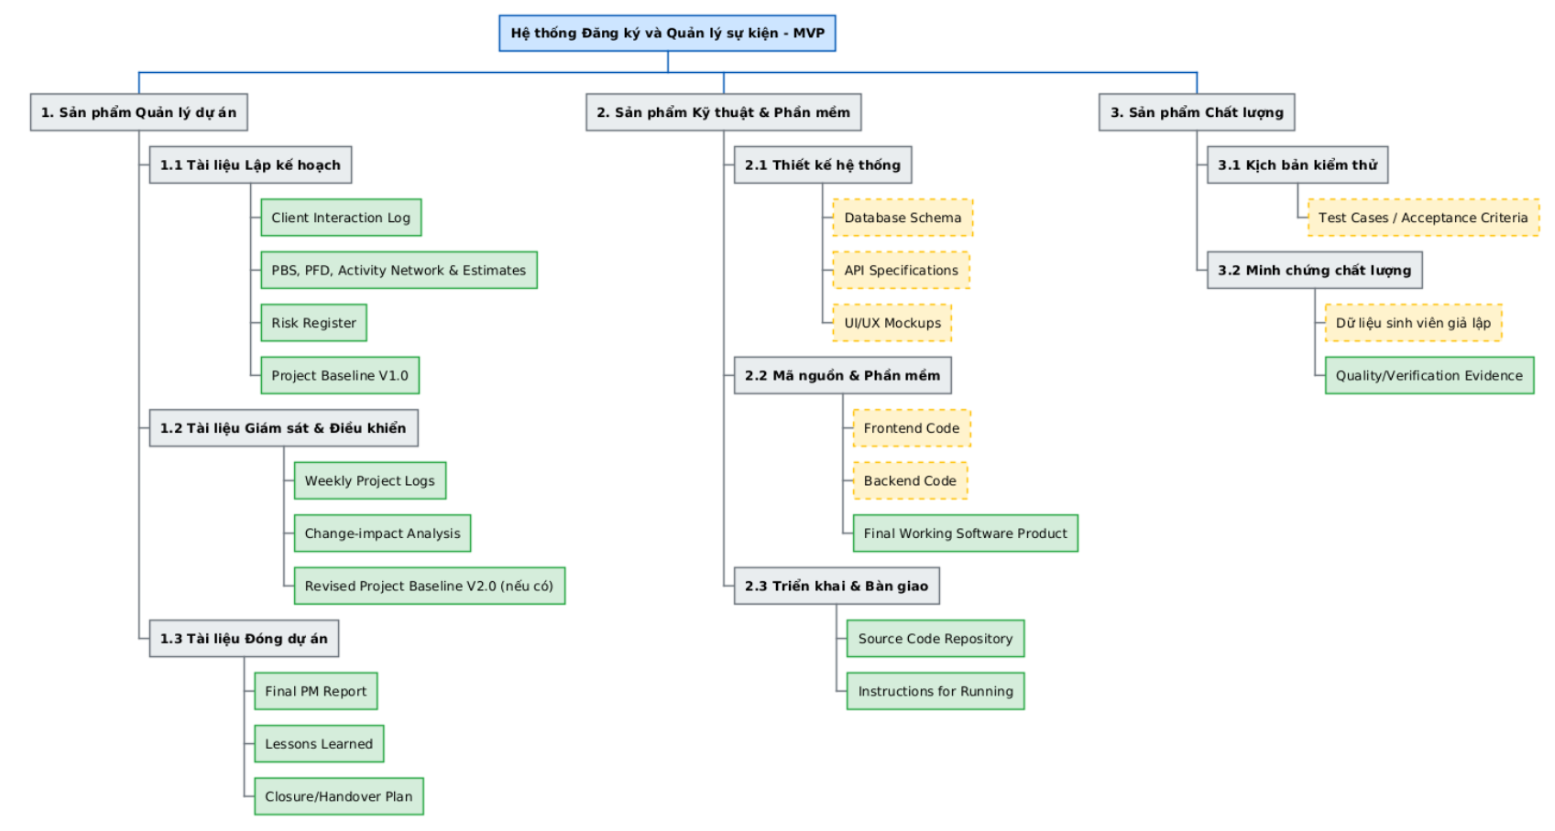
\includegraphics[width=\linewidth]{Images/PBS.png}
\end{adjustbox}
\captionsetup{aboveskip=3pt}
\caption{Cấu trúc phân rã sản phẩm của dự án}
\end{figure}

\noindent Ô xanh, viền liền: deliverable. Ô vàng, viền đứt: intermediate. Đường nối biểu diễn quan hệ phân rã, không biểu diễn thứ tự thực hiện.
\end{landscape}
\restoregeometry
\subsubsection{Phân biệt Deliverable products và Intermediate products}
Theo phương pháp Step Wise, việc phân định rõ hai loại sản phẩm này giúp nhóm tập trung nguồn lực vào các hạng mục cốt lõi cần nghiệm thu, đồng thời kiểm soát hiệu quả các công cụ hỗ trợ trong quá trình phát triển. Trong sơ đồ PBS, sự khác biệt này được trực quan hóa bằng màu sắc (xanh lá/vàng) và định dạng viền (liền/đứt). Căn cứ phân loại chi tiết được trình bày trong bảng sau:

\begin{table}[H]
\centering
\caption{Phân biệt sản phẩm bàn giao và sản phẩm trung gian}
\small
\renewcommand{\arraystretch}{1.25}
\begin{tabularx}{\textwidth}{|p{2cm}|>{\raggedright\arraybackslash}X|>{\raggedright\arraybackslash}X|}
\hline
\textbf{Tiêu chí} & \textbf{Sản phẩm bàn giao (Deliverable Products)(Ký hiệu: Ô màu xanh lá, nét liền)} & \textbf{Sản phẩm trung gian (Intermediate Products)(Ký hiệu: Ô màu vàng, nét đứt)} \\ \hline
Định nghĩa \& Tính chất & Là những sản phẩm đích bắt buộc phải hoàn thành và bàn giao để nghiệm thu ở các mốc của dự án. & Là các sản phẩm nội bộ, đóng vai trò làm đầu vào, công cụ kiểm soát hoặc thành phần cấu tạo để tạo ra sản phẩm bàn giao. \\ \hline
Căn cứ xác định & Xác định dựa trên danh sách "Expected outputs" và "Submission Requirements" của đề bài. Đây là minh chứng bắt buộc để đánh giá năng lực áp dụng quy trình quản lý dự án. & Xác định dựa trên quy trình phối hợp làm việc thực tế của nhóm (BA, Dev, QA) để xây dựng hệ thống. \\ \hline
Ví dụ nhóm Quản lý dự án & Toàn bộ tài liệu PM được xem là Deliverable vì là tiêu chí chấm điểm cốt lõi: Project Baseline V1.0, PBS, PFD, Estimates, Risk Register, Weekly Logs. & Các bản nháp, biên bản họp nội bộ (không yêu cầu nộp) được dùng để xây dựng kế hoạch chính thức. \\ \hline
Ví dụ nhóm Kỹ thuật \& Chất lượng & Final Working Software Product, Quality Evidence, Source Code Repository, Instructions for Running. & Database Schema, Mã nguồn Frontend/Backend, Test Cases, Dữ liệu giả lập. \\ \hline
\end{tabularx}
\end{table}

\subsection{Prepare Product Descriptions (PDs)}


Dựa trên cấu trúc PBS đã xác định, nhóm tiến hành lập Bảng mô tả sản phẩm (Product Descriptions - PDs) cho 5 sản phẩm cốt lõi nhất đại diện cho 3 nhóm: Quản lý dự án, Kỹ thuật và Chất lượng. Các mô tả này tuân thủ phương pháp hoạch định định hướng sản phẩm của Step Wise, đảm bảo tính chặt chẽ trong việc kiểm soát chất lượng, nguồn lực và theo dõi tiến độ của dự án.

% ==========================================
% PD 1: PROJECT BASELINE V1.0
% ==========================================
\clearpage
\begin{table}[H]
    \centering
    \caption{Product Description: Project Baseline V1.0}
    \renewcommand{\arraystretch}{1.5}
    \begin{tabularx}{\textwidth}{|>{\hsize=0.5\hsize\linewidth=\hsize\bfseries}X|>{\hsize=1.5\hsize\linewidth=\hsize}X|}
        \hline
        Product Identity & \textbf{Project Baseline V1.0} (Đường cơ sở dự án phiên bản 1.0) \\
        \hline
        Description & Đây là tài liệu kế hoạch nền tảng đã được nhóm và khách hàng thống nhất, dùng làm mốc đối chiếu để giám sát tiến độ, công sức, chi phí và phạm vi trong suốt quá trình thực thi dự án. \\
        \hline
        Derivation & Được tổng hợp từ Project brief, Client Interaction Log, phạm vi đã thống nhất và các sản phẩm lập kế hoạch Task 2. \\
        \hline
        Composition & 
        \vspace{-0.8em}
        \begin{itemize}[leftmargin=*, nosep]
            \item PBS, PFD và các bảng mô tả sản phẩm (PDs).
            \item Mạng lưới hoạt động và các điểm kiểm tra (Checkpoints).
            \item Danh sách rủi ro cấp hoạt động và biện pháp ứng phó.
            \item Kế hoạch phân bổ nguồn lực và đảm bảo chất lượng.
            \item Lịch biểu và dự toán chi phí/công sức (Schedule and cost baseline).
        \end{itemize}
        \vspace{-1em} \\
        \hline
        Format & Báo cáo dạng văn bản PDF (kết hợp bảng biểu, sơ đồ) và được lưu trữ trên không gian làm việc Confluence của dự án. \\
        \hline
        Relevant Standards & Tuân thủ phương pháp lập kế hoạch Step Wise, nguyên tắc truy vết (Traceability) trong quản lý dự án phần mềm, và chuẩn quản lý tài liệu nội bộ. \\
        \hline
        Quality Criteria & 
        \vspace{-0.8em}
        \begin{itemize}[leftmargin=*, nosep]
            \item Được nhóm rà soát và Đại diện khách hàng xem xét, phê duyệt theo thẩm quyền; chỉ ghi đã duyệt khi có xác nhận.
            \item Các ước lượng phải phân biệt rõ công sức (effort) và thời gian trôi qua (elapsed time).
            \item Có tính khả thi về mặt phân bổ nguồn lực (phù hợp với quy mô nhóm triển khai).
            \item Cung cấp đầy đủ biện pháp giảm thiểu và dự phòng cho các rủi ro quan trọng.
        \end{itemize}
        \vspace{-1em} \\
        \hline
    \end{tabularx}
\end{table}

% ==========================================
% PD 2: DATABASE SCHEMA
% ==========================================
\clearpage
\begin{table}[H]
    \centering
    \caption{Product Description: Database Schema}
    \renewcommand{\arraystretch}{1.5}
    \begin{tabularx}{\textwidth}{|>{\hsize=0.5\hsize\linewidth=\hsize\bfseries}X|>{\hsize=1.5\hsize\linewidth=\hsize}X|}
        \hline
        Product Identity & \textbf{Database Schema} (Lược đồ Cơ sở dữ liệu) \\
        \hline
        Description & Bản thiết kế cấu trúc lưu trữ dữ liệu tập trung, định nghĩa cách hệ thống quản lý thông tin sự kiện, người dùng, trạng thái đăng ký, danh sách chờ và kết quả điểm danh. \\
        \hline
        Derivation & Bắt nguồn từ các quy tắc nghiệp vụ (Business rules) do bộ phận Phân tích nghiệp vụ thu thập, ma trận phân quyền người dùng, và yêu cầu dữ liệu của luồng đăng ký/waitlist. \\
        \hline
        Composition & 
        \vspace{-0.8em}
        \begin{itemize}[leftmargin=*, nosep]
            \item Các thực thể chính (Event, User, Registration, Attendance).
            \item Thuộc tính, Kiểu dữ liệu, Khóa chính (PK) / Khóa ngoại (FK).
            \item Ràng buộc toàn vẹn (ví dụ: ngăn đăng ký trùng cùng một sự kiện).
        \end{itemize}
        \vspace{-1em} \\
        \hline
        Format & Sơ đồ thực thể kết hợp (ERD) và mã lệnh SQL (DDL) khởi tạo bảng. \\
        \hline
        Relevant Standards & Chuẩn hóa cơ sở dữ liệu quan hệ (ít nhất đạt chuẩn 3NF), quy tắc đặt tên (Coding Conventions) thống nhất, và cú pháp chuẩn của PostgreSQL. \\
        \hline
        Quality Criteria & 
        \vspace{-0.8em}
        \begin{itemize}[leftmargin=*, nosep]
            \item Bao quát các trường bắt buộc đã thống nhất; có PK/FK và ràng buộc duy nhất cho cặp sinh viên--sự kiện để chống đăng ký trùng.
            \item Script DDL thực thi thành công trên PostgreSQL với cơ sở dữ liệu sạch.
            \item Có dữ liệu xác định thứ tự FIFO. Quy tắc sức chứa và chuyển waitlist được kiểm chứng cùng xử lý giao dịch của Backend.
        \end{itemize}
        \vspace{-1em} \\
        \hline
    \end{tabularx}
\end{table}

% ==========================================
% PD 3: TEST CASES & ACCEPTANCE CRITERIA
% ==========================================
\clearpage
\begin{table}[H]
    \centering
    \caption{Product Description: Test Cases \& Acceptance Criteria}
    \renewcommand{\arraystretch}{1.5}
    \begin{tabularx}{\textwidth}{|>{\hsize=0.5\hsize\linewidth=\hsize\bfseries}X|>{\hsize=1.5\hsize\linewidth=\hsize}X|}
        \hline
        Product Identity & \textbf{Test Cases \& Acceptance Criteria} (Kịch bản kiểm thử \& Tiêu chí chấp nhận) \\
        \hline
        Description & Tập hợp các điều kiện và thao tác giả lập để kiểm chứng hệ thống phần mềm có đáp ứng đúng các yêu cầu chức năng, yêu cầu bảo mật và quy trình vận hành đã cam kết hay không. \\
        \hline
        Derivation & Dựa trên Phạm vi dự án (Project Scope), Ma trận phân quyền, và bộ các thước đo hiệu quả (Measures of Effectiveness). \\
        \hline
        Composition & Mỗi TC có mã TC, mã yêu cầu, tên tính năng, tiền điều kiện, dữ liệu, các bước và kết quả mong đợi. Khi thực thi, ghi kết quả thực tế, Pass/Fail và liên kết bằng chứng. Bao gồm Happy path và ngoại lệ: hết chỗ, đăng ký trùng, chuyển waitlist và lỗi kết nối mạng. \\
        \hline
        Format & Lưu trữ dưới dạng tài liệu trên nền tảng Confluence và được quản lý thành các task kiểm thử trên hệ thống Jira Software. \\
        \hline
        Relevant Standards & Tuân thủ Định nghĩa hoàn thành (Definition of Done - DoD) của quy trình phát triển dự án. \\
        \hline
        Quality Criteria & 
        \vspace{-0.8em}
        \begin{itemize}[leftmargin=*, nosep]
            \item Mỗi yêu cầu cốt lõi của MVP có TC tương ứng, gồm luồng chính và các tình huống ngoại lệ phù hợp.
            \item Mô tả rõ ràng, đơn nghĩa, cho phép thực hiện kiểm tra chéo (Cross-testing) bởi bất kỳ thành viên nào trong nhóm.
            \item Chứa các test case giả định sai lệch để xác minh khả năng chặn lỗi (validation) của hệ thống.
        \end{itemize}
        \vspace{-1em} \\
        \hline
    \end{tabularx}
\end{table}
% ==========================================
% PD 4: FINAL WORKING SOFTWARE PRODUCT
% ==========================================
\clearpage
\begin{table}[H]
    \centering
    \caption{Product Description: Final Working Software Product}
    \renewcommand{\arraystretch}{1.5}
    \begin{tabularx}{\textwidth}{|>{\hsize=0.5\hsize\linewidth=\hsize\bfseries}X|>{\hsize=1.5\hsize\linewidth=\hsize}X|}
        \hline
        Product Identity & \textbf{Final Working Software Product} (Phần mềm hệ thống đăng ký và quản lý sự kiện) \\
        \hline
        Description & Phần mềm MVP hỗ trợ quy trình khép kín (end-to-end): tạo sự kiện, đăng ký/hủy và waitlist, điểm danh QR hoặc thủ công, báo cáo và xuất CSV/Excel. Sử dụng dữ liệu sinh viên giả lập theo phạm vi đã thống nhất. \\
        \hline
        Derivation & Được phát triển dựa trên Đường cơ sở dự án (Project Baseline), thiết kế giao diện (UI/UX Mockups), Đặc tả API (API Specifications) và các đoạn mã nguồn cấu thành. \\
        \hline
        Composition & 
        \vspace{-0.8em}
        \begin{itemize}[leftmargin=*, nosep]
            \item Hệ thống Frontend (Angular) cho giao diện của 3 nhóm người dùng.
            \item Backend API (Java Spring Boot) xử lý logic nghiệp vụ.
            \item Cơ sở dữ liệu lưu trữ tập trung PostgreSQL.
            \item Email xác nhận đăng ký, thay đổi quan trọng của sự kiện và chuyển từ waitlist sang danh sách chính thức.
        \end{itemize}
        \vspace{-1em} \\
        \hline
        Format & Ứng dụng được triển khai trên máy chủ đám mây (AWS Lightsail) và có thể truy cập, thao tác trực tiếp qua trình duyệt web. \\
        \hline
        Relevant Standards & Tiêu chuẩn Clean Code, quy định nộp và tích hợp mã nguồn (Pull Request) trên hệ thống GitHub, và các ràng buộc bảo vệ quyền riêng tư của dữ liệu người dùng. \\
        \hline
        Quality Criteria & 
        \vspace{-0.8em}
        \begin{itemize}[leftmargin=*, nosep]
            \item Ứng dụng biên dịch thành công; các luồng nghiệm thu đã thống nhất chạy được trên môi trường kiểm thử được ghi nhận.
            \item Thể hiện luồng công việc mạch lạc (coherent end-to-end workflows), các tính năng liên kết chặt chẽ thay vì chỉ là các màn hình rời rạc.
            \item Mã nguồn phải qua quy trình kiểm duyệt (Peer Code Review) và được chấp thuận (Approve) từ ít nhất một thành viên khác.
            \item Đạt toàn bộ TC nghiệm thu cốt lõi đã chốt; không còn lỗi nghiêm trọng làm gián đoạn các luồng này.
        \end{itemize}
        \vspace{-1em} \\
        \hline
    \end{tabularx}
\end{table}

% ==========================================
% PD 5: FINAL PROJECT MANAGEMENT REPORT
% ==========================================
\clearpage
\begin{table}[H]
    \centering
    \caption{Product Description: Final Project Management Report}
    \renewcommand{\arraystretch}{1.5}
    \begin{tabularx}{\textwidth}{|>{\hsize=0.5\hsize\linewidth=\hsize\bfseries}X|>{\hsize=1.5\hsize\linewidth=\hsize}X|}
        \hline
        Product Identity & \textbf{Final Project Management Report} (Báo cáo Quản lý dự án cuối kỳ) \\
        \hline
        Description & Báo cáo phân tích và tổng kết hiệu suất thực tế của toàn bộ vòng đời dự án, đối chiếu kế hoạch gốc với kết quả triển khai thực tế, đồng thời rút ra bài học kinh nghiệm (Lessons Learned) cho các dự án tương lai. \\
        \hline
        Derivation & Tổng hợp dữ liệu thực tế từ hồ sơ giám sát hàng tuần (Weekly Logs), Project Baseline V1.0 (và V2.0 nếu có), Nhật ký rủi ro (Risk Register), và dữ liệu từ các quy trình quản lý thay đổi. \\
        \hline
        Composition & 
        \vspace{-0.8em}
        \begin{itemize}[leftmargin=*, nosep]
            \item Bảng đối chiếu Kế hoạch so với Thực tế (công sức, lịch biểu, chi phí, phạm vi, chất lượng).
            \item Phân tích sai số ước lượng và các quyết định quản lý đã đưa ra.
            \item Đánh giá mức độ đạt các mục tiêu nghiệp vụ (Effectiveness measures).
            \item Closure/Handover Plan và Lessons Learned; phụ lục hoặc liên kết đóng góp và reflection cá nhân.
        \end{itemize}
        \vspace{-1em} \\
        \hline
        Format & Báo cáo định dạng văn bản PDF, kết hợp các biểu đồ so sánh trực quan, được lưu trữ trên hệ thống quản lý tài liệu tập trung của dự án. \\
        \hline
        Relevant Standards & Định dạng chuẩn của báo cáo tổng kết dự án chuyên nghiệp, tuân thủ nguyên tắc trung thực và tính khả truy (Traceability) xuyên suốt các tài liệu dự án. \\
        \hline
        Quality Criteria & 
        \vspace{-0.8em}
        \begin{itemize}[leftmargin=*, nosep]
            \item Có lập luận chặt chẽ (justification) và bằng chứng cụ thể cho mọi độ lệch về tiến độ và công sức.
            \item Dữ liệu báo cáo nhất quán tuyệt đối với các bản ghi nhận tiến độ (logs) hàng tuần.
            \item Tách biệt rõ ràng phần đánh giá mức độ hoàn thành chức năng phần mềm với phần đánh giá mục tiêu kinh doanh/nghiệp vụ tổng thể.
            \item Bài học kinh nghiệm thực tế, mang tính ứng dụng cao.
        \end{itemize}
        \vspace{-1em} \\
        \hline
    \end{tabularx}
\end{table}

\clearpage
\subsection{Construct a Product Flow Diagram (PFD)}
PFD thể hiện phụ thuộc giữa các sản phẩm ở PBS 2.1 và PDs 2.2. Mũi tên đi từ sản phẩm đầu vào đến sản phẩm sử dụng đầu vào đó. Ba increment dưới đây là các instance tích lũy của phần mềm.
\begin{table}[H]
\centering
\caption{Các instance phần mềm}
\renewcommand{\arraystretch}{1.3}
\begin{tabularx}{\textwidth}{|p{2.5cm}|X|}
\hline
\textbf{Instance} & \textbf{Phạm vi} \\ \hline
Increment 1 & Tài khoản, phân quyền, quản lý và tìm/xem sự kiện. \\ \hline
Increment 2 & Kế thừa I1; thêm đăng ký/hủy, waitlist và email. \\ \hline
Increment 3 & Kế thừa I2; thêm điểm danh QR/thủ công, báo cáo và xuất CSV/Excel. \\ \hline
\end{tabularx}
\end{table}
Ô xanh là deliverable; ô vàng là intermediate; ô xám là đầu vào bên ngoài. Nét đứt của mũi tên là phụ thuộc có điều kiện. Chấm đen là điểm nối; các đường giao nhau không có chấm không nối với nhau.

\newgeometry{margin=1cm,includefoot}
\begin{landscape}
\landscapeheader
\begin{figure}[H]
\centering
\begin{adjustbox}{max width=.98\linewidth,max totalheight=.70\textheight}
\begin{tikzpicture}[x=1cm,y=1cm]
\draw[flowshaft] (1.2000,-6.2000) -- (0.8000,-6.2000);
\draw[flowshaft] (0.8000,-6.2000) -- (0.8000,-15.3000);
\draw[flow] (0.8000,-10.0000) -- (1.2000,-10.0000);
\draw[flow] (0.8000,-15.3000) -- (1.2000,-15.3000);
\draw[flow] (9.5000,-0.7250) -- (9.5000,-1.0000) -- (4.0000,-1.0000) -- (4.0000,-1.4000);
\draw[flow] (12.0000,-0.7250) -- (12.0000,-1.4500);
\draw[flow] (14.5000,-0.7250) -- (14.5000,-1.0000) -- (20.0000,-1.0000) -- (20.0000,-1.5500);
\draw[flow] (4.0000,-2.6000) -- (4.0000,-3.6500);
\draw[flow] (12.0000,-2.5500) -- (12.0000,-3.6000);
\draw[flow] (14.8000,-2.0000) -- (15.8000,-2.0000) -- (15.8000,-3.0000) -- (18.6000,-3.0000) -- (18.6000,-3.6500);
\draw[flow] (20.0000,-2.4500) -- (20.0000,-3.6500);
\draw[flow] (6.8000,-4.1000) -- (9.2000,-4.1000);
\draw[flow] (12.0000,-4.6000) -- (12.0000,-5.7000);
\draw[flow] (17.2000,-2.0000) -- (16.4000,-2.0000) -- (16.4000,-5.9500) -- (14.8000,-5.9500);
\draw[flow] (20.0000,-4.5500) -- (20.0000,-5.2000) -- (13.4000,-5.2000) -- (13.4000,-5.7000);
\draw[flow] (12.0000,-6.7000) -- (12.0000,-7.4000);
\draw[flow] (12.0000,-8.4000) -- (12.0000,-9.5000);
\draw[flow] (14.8000,-6.4500) -- (16.6000,-6.4500) -- (16.6000,-9.7500) -- (17.2000,-9.7500);
\draw[flow] (14.8000,-7.9000) -- (16.1000,-7.9000) -- (16.1000,-10.0000) -- (17.2000,-10.0000);
\draw[flow] (14.8000,-10.2500) -- (17.2000,-10.2500);
\draw[flow] (12.0000,-10.5000) -- (12.0000,-11.6000);
\draw[flow] (20.0000,-10.5000) -- (20.0000,-11.0000) -- (13.4000,-11.0000) -- (13.4000,-11.6000);
\draw[flow] (4.0000,-4.5500) -- (4.0000,-5.7500);
\draw[flow] (6.8000,-4.3250) -- (7.5000,-4.3250) -- (7.5000,-9.0000) -- (5.4000,-9.0000) -- (5.4000,-9.5000);
\draw[flow] (4.0000,-8.3500) -- (4.0000,-9.5000);
\draw[flow, densely dashed] (4.0000,-10.5000) -- (4.0000,-11.6500);
\draw[flow] (1.2000,-4.1000) -- (0.4000,-4.1000) -- (0.4000,-14.7000) -- (1.2000,-14.7000);
\draw[flow] (6.8000,-10.0000) -- (7.6000,-10.0000) -- (7.6000,-13.4000) -- (2.6000,-13.4000) -- (2.6000,-14.4000);
\draw[flow, densely dashed] (4.0000,-12.5500) -- (4.0000,-14.4000);
\draw[flow] (14.8000,-12.1000) -- (17.2000,-12.1000);
\draw[flow] (12.0000,-12.6000) -- (12.0000,-14.5500);
\draw[flow] (20.0000,-12.6000) -- (20.0000,-13.9000) -- (13.4000,-13.9000) -- (13.4000,-14.5500);
\draw[flow] (9.2000,-12.1000) -- (8.2000,-12.1000) -- (8.2000,-13.9000) -- (5.4000,-13.9000) -- (5.4000,-14.4000);
\draw[flow] (9.2000,-15.0000) -- (6.8000,-15.0000);
\fill[black!85] (0.8000,-10.0000) circle[radius=1.5pt];
\node[deliverable,text width=280.428pt,minimum height=0.650cm,font=\fontsize{9}{10.8}\selectfont] (scope) at (12.0000,-0.4000) {Phạm vi MVP và Client Interaction Log};
\node[deliverable,text width=155.235pt,minimum height=1.200cm,font=\fontsize{9}{10.8}\selectfont] (plan) at (4.0000,-2.0000) {Bộ kế hoạch: PBS, PDs, PFD, AON\\Ước lượng, rủi ro, nguồn lực, lịch};
\node[intermediate,text width=155.235pt,minimum height=1.100cm,font=\fontsize{9}{10.8}\selectfont] (design) at (12.0000,-2.0000) {Database Schema\\API Specifications; UI/UX Mockups};
\node[intermediate,text width=155.235pt,minimum height=0.900cm,font=\fontsize{9}{10.8}\selectfont] (tests) at (20.0000,-2.0000) {Test Cases / Acceptance Criteria};
\node[deliverable,text width=155.235pt,minimum height=0.900cm,font=\fontsize{9}{10.8}\selectfont] (baseline) at (4.0000,-4.1000) {Project Baseline V1.0};
\node[intermediate,text width=155.235pt,minimum height=1.000cm,font=\fontsize{9}{10.8}\selectfont] (code) at (12.0000,-4.1000) {Frontend / Backend Code\\và cấu hình triển khai};
\node[intermediate,text width=155.235pt,minimum height=0.900cm,font=\fontsize{9}{10.8}\selectfont] (data) at (20.0000,-4.1000) {Dữ liệu sinh viên và nghiệp vụ giả lập};
\node[deliverable,text width=155.235pt,minimum height=0.900cm,font=\fontsize{9}{10.8}\selectfont] (logs) at (4.0000,-6.2000) {Weekly Project Logs tuần k\\Risk Register cập nhật};
\node[intermediate,text width=155.235pt,minimum height=1.000cm,font=\fontsize{9}{10.8}\selectfont] (i1) at (12.0000,-6.2000) {Increment 1 đã kiểm thử};
\node[external,text width=155.235pt,minimum height=0.900cm,font=\fontsize{9}{10.8}\selectfont] (event) at (4.0000,-7.9000) {Change/event};
\node[intermediate,text width=155.235pt,minimum height=1.000cm,font=\fontsize{9}{10.8}\selectfont] (i2) at (12.0000,-7.9000) {Increment 2 đã kiểm thử};
\node[deliverable,text width=155.235pt,minimum height=1.000cm,font=\fontsize{9}{10.8}\selectfont] (decision) at (4.0000,-10.0000) {Change-impact Analysis\\và Management Decision Record};
\node[intermediate,text width=155.235pt,minimum height=1.000cm,font=\fontsize{9}{10.8}\selectfont] (i3) at (12.0000,-10.0000) {Increment 3 đã kiểm thử};
\node[deliverable,text width=155.235pt,minimum height=1.000cm,font=\fontsize{9}{10.8}\selectfont] (evidence) at (20.0000,-10.0000) {Quality/Verification Evidence\\kết quả I1, I2 và I3};
\node[deliverable,text width=155.235pt,minimum height=0.900cm,font=\fontsize{9}{10.8}\selectfont] (v2) at (4.0000,-12.1000) {Revised Project Baseline V2.0\\nếu được duyệt sửa baseline};
\node[deliverable,text width=155.235pt,minimum height=1.000cm,font=\fontsize{9}{10.8}\selectfont] (final) at (12.0000,-12.1000) {Final Working Software Product};
\node[deliverable,text width=155.235pt,minimum height=1.000cm,font=\fontsize{9}{10.8}\selectfont] (repo) at (20.0000,-12.1000) {Source Code Repository\\Instructions for Running};
\node[deliverable,text width=155.235pt,minimum height=1.200cm,font=\fontsize{9}{10.8}\selectfont] (report) at (4.0000,-15.0000) {Final PM Report\\gồm Closure Plan, Lessons Learned\\và phụ lục cá nhân};
\node[deliverable,text width=155.235pt,minimum height=0.900cm,font=\fontsize{9}{10.8}\selectfont] (closure) at (12.0000,-15.0000) {Closure/Handover Plan};
\end{tikzpicture}
\end{adjustbox}
\captionsetup{aboveskip=3pt}
\caption{PFD tổng thể của dự án}
\end{figure}

\noindent Test cases, dữ liệu và mã nguồn được dùng lại/cập nhật qua ba increment. Quality Evidence và logs tích lũy theo từng đợt/tuần. V2.0 chỉ có khi được duyệt sửa baseline. Lessons Learned và reflection là thành phần báo cáo; Closure Plan có trước bản chốt Final PM Report theo PD 2.2.
\end{landscape}
\restoregeometry

\subsection{Derive activities and construct the ideal network}
Các hoạt động được suy ra từ sản phẩm trong PFD và đặt tên theo dạng động từ + danh từ. Mạng AON xét phụ thuộc logic; checkpoint ở 2.5 và effort cùng phân công sơ bộ ở 2.6. Lịch theo nguồn lực được xây dựng ở 2.10--2.11.
\subsubsection{Hoạt động kỹ thuật và bàn giao}
\begin{table}[H]
\centering
\caption{Hoạt động kỹ thuật, kiểm thử, tổng kết và bàn giao}
\footnotesize
\renewcommand{\arraystretch}{1.25}
\begin{tabularx}{\linewidth}{|p{0.8cm}|p{2.6cm}|>{\raggedright\arraybackslash}X|p{2.2cm}|}
\hline
\textbf{Mã} & \textbf{Hoạt động} & \textbf{Sản phẩm/kết quả} & \textbf{Tiền nhiệm/điều kiện} \\ \hline
A01 & Thiết kế CSDL, giao diện và API & Database Schema; API Specifications; UI/UX Mockups & G01 đã có \\ \hline
A02 & Xây dựng test case và tiêu chí chấp nhận & Test Cases / Acceptance Criteria & G01 đã có \\ \hline
A03 & Thiết lập môi trường triển khai & Cấu hình PostgreSQL, email và triển khai & G04, A01 \\ \hline
A04 & Tạo dữ liệu kiểm thử giả lập & Dữ liệu sinh viên và nghiệp vụ giả lập & A01, A02 \\ \hline
A05 & Lập trình tài khoản và quản lý sự kiện & Frontend/Backend phiên bản Increment 1 & A03 \\ \hline
A06 & Kiểm thử và sửa lỗi đợt 1 & Increment 1 đã kiểm thử; Quality Evidence I1 & A04, A05 \\ \hline
A07 & Lập trình đăng ký/hủy, waitlist và email & Frontend/Backend phiên bản Increment 2 & A06 \\ \hline
A08 & Kiểm thử và sửa lỗi đợt 2 & Increment 2 đã kiểm thử; Quality Evidence I2 & A07 \\ \hline
A09 & Lập trình chức năng điểm danh & Phân hệ QR và điểm danh thủ công & A08 \\ \hline
A10 & Lập trình báo cáo và xuất CSV/Excel & Phân hệ báo cáo và xuất tệp & A08 \\ \hline
A11 & Tích hợp và triển khai bản nghiệm thu & Release candidate Increment 3 trên Lightsail & A09, A10 \\ \hline
A12 & Kiểm thử nghiệm thu và sửa lỗi & Increment 3; Final Software; Quality Evidence & A11 \\ \hline
A13 & Chốt phiên bản mã nguồn bàn giao & Source Code Repository có commit/release tag & A12 \\ \hline
A14 & Hoàn thiện và xác minh hướng dẫn chạy & Instructions for Running đã xác minh & A13 \\ \hline
A15 & Phân tích hiệu suất dự án và rút bài học & Phân tích planned-versus-actual; Lessons Learned & A12, G06, G07 \\ \hline
A16 & Hoàn thiện kế hoạch đóng và bàn giao & Closure/Handover Plan & A14, A15 \\ \hline
A19 & Hoàn thiện đóng góp cá nhân và diễn tập demo & Contribution/reflection statements; kịch bản demo & A12 \\ \hline
A18 & Chốt báo cáo quản lý dự án cuối kỳ & Final PM Report, gồm Closure Plan và phụ lục & A16, A19 \\ \hline
A17 & Bàn giao và trình diễn sản phẩm & Bộ sản phẩm theo PBS; biên bản bàn giao & A18 \\ \hline
\end{tabularx}
\end{table}

\noindent A05, A07, A09 và A10 gồm Frontend/Backend, unit test và peer review; A06, A08 và A12 gồm sửa lỗi, retest và Quality Evidence. PM hỗ trợ Backend; BA hỗ trợ UI/Frontend; BE/FE giữ đầu mối kỹ thuật. Phân công ở 2.6 không đổi sản phẩm hoặc phụ thuộc logic. A15 tạo phân tích/bài học; A18 chốt báo cáo sau Closure Plan và reflection.
\newpage
\subsubsection{Hoạt động lập kế hoạch và kiểm soát}
\begin{table}[H]
\centering
\caption{Hoạt động lập kế hoạch, theo dõi và quản lý thay đổi}
\footnotesize
\renewcommand{\arraystretch}{1.25}
\begin{tabularx}{\linewidth}{|p{0.8cm}|p{2.6cm}|>{\raggedright\arraybackslash}X|p{2.2cm}|}
\hline
\textbf{Mã} & \textbf{Hoạt động} & \textbf{Sản phẩm/kết quả} & \textbf{Tiền nhiệm/điều kiện} \\ \hline
G01 & Ghi nhận và làm rõ yêu cầu khách hàng & Client Interaction Log; phạm vi đã thống nhất & Project brief; đã thực hiện ở Task 1 \\ \hline
G02 & Xác định và mô tả sản phẩm, phụ thuộc & PBS; PDs; PFD; Activity Network & G01 đã có \\ \hline
G03 & Ước lượng và lập kế hoạch nguồn lực, rủi ro & Estimates; Risk Register; kế hoạch lịch/chi phí & G02 \\ \hline
G04 & Tổng hợp và trình duyệt kế hoạch gốc & Project Baseline V1.0 & G03; rà soát và phê duyệt \\ \hline
G05 & Theo dõi và ghi log tiến độ tuần k & Weekly Project Log tuần k & G04; dữ liệu thực hiện tuần k \\ \hline
G06 & Rà soát rủi ro và cập nhật trao đổi tuần k & Risk Register; Client Interaction Log cập nhật & G05; vấn đề và trao đổi mới \\ \hline
G07 & Phân tích tác động thay đổi và ghi quyết định & Change-impact Analysis; Management Decision Record & G04; change/event; hồ sơ hiện có \\ \hline
G08 & Cập nhật baseline theo quyết định được duyệt & Revised Project Baseline V2.0; lưu cả V1.0 & G07; được duyệt sửa baseline \\ \hline
\end{tabularx}
\end{table}

G01 và kết quả Task 1 là đầu vào đã có; các phần đã hoàn thành được kế thừa. G02--G04 hoàn thiện baseline sau các bước lập kế hoạch liên quan. G05 và G06 thực hiện theo tuần; G07 xử lý change/event do giảng viên giao, sử dụng baseline và hồ sơ hiện có. G08 nằm ngoài AON cơ sở, chỉ phát sinh nếu được duyệt sửa baseline. Khi đó bổ sung G08 và các phụ thuộc liên quan vào mạng cập nhật V2.0; A15 sử dụng cả hồ sơ thay đổi đã duyệt.

\noindent Trên AON, hai nút tổng hợp G02--G04 và G05--G07 rút gọn cách trình bày; chi tiết vẫn giữ ở bảng trên. Nút G02--G04 kết thúc tại G04/CP0. G05--G07 không chặn các nhánh lập trình. Khi lập lịch, dùng các hoạt động G chi tiết và giờ công ở 2.6; không cộng thêm giờ cho nút tổng hợp.

\medskip
\noindent A04 không chặn A05; dữ liệu cần sẵn sàng trước A06. A09 và A10 có thể làm song song trước A11. A14, A15 và A19 có thể chuẩn bị song song khi đầu vào sẵn sàng. Các nút tài liệu cuối kỳ biểu diễn việc hoàn tất; bản nháp có thể được chuẩn bị sớm.
\clearpage
\newgeometry{margin=1cm,includefoot}
\begin{landscape}
\landscapeheader
\subsubsection{Ideal Activity Network (AON)}
Mũi tên liền biểu diễn phụ thuộc finish-to-start; Start là mốc thời lượng 0. CP đánh dấu review trước khi mở nhánh phụ thuộc (mục 2.5). G01/Task 1 là đầu vào đã có; G08 có điều kiện, nằm ngoài mạng cơ sở.
\begin{figure}[H]
\centering
\begin{adjustbox}{max width=.98\linewidth,max totalheight=.66\textheight}
\begin{tikzpicture}[x=1cm,y=1cm]
\draw[flow] (12.7000,0.4000) -- (3.5000,0.4000) -- (3.5000,-3.4000);
\draw[flow] (13.7000,0.0500) -- (13.7000,-0.4000) -- (10.3000,-0.4000) -- (10.3000,-0.8300);
\draw[flow] (14.7000,0.4000) -- (23.9000,0.4000) -- (23.9000,-0.8300);
\draw[flow] (6.1000,-4.0000) -- (7.7000,-4.0000);
\draw[flow] (3.5000,-4.6000) -- (3.5000,-7.7200);
\draw[flow] (3.5000,-8.9200) -- (3.5000,-12.1900);
\draw[flow] (10.3000,-1.7300) -- (10.3000,-3.5500);
\draw[flow] (12.9000,-1.2800) -- (20.0000,-1.2800) -- (20.0000,-2.8000) -- (22.6000,-2.8000) -- (22.6000,-3.5500);
\draw[flow] (23.9000,-1.7300) -- (23.9000,-3.5500);
\draw[flow] (10.3000,-4.4500) -- (10.3000,-4.9900);
\draw[flow] (23.9000,-4.4500) -- (23.9000,-4.6400) -- (17.1000,-4.6400) -- (17.1000,-4.9900);
\draw[flow] (12.9000,-5.4400) -- (14.5000,-5.4400);
\draw[flow] (17.1000,-5.8900) -- (17.1000,-6.4300);
\draw[flow] (19.7000,-6.8800) -- (21.3000,-6.8800);
\draw[flow] (22.6000,-7.3300) -- (22.6000,-7.5600) -- (17.1000,-7.5600) -- (17.1000,-7.8700);
\draw[flow] (23.9000,-7.3300) -- (23.9000,-7.8700);
\draw[flow] (17.1000,-8.7700) -- (17.1000,-9.0400) -- (19.2000,-9.0400) -- (19.2000,-9.3100);
\draw[flow] (23.9000,-8.7700) -- (23.9000,-9.0400) -- (21.8000,-9.0400) -- (21.8000,-9.3100);
\draw[flow] (20.5000,-10.2100) -- (20.5000,-10.7500);
\draw[flow] (19.2000,-11.6500) -- (19.2000,-11.7600) -- (4.8000,-11.7600) -- (4.8000,-12.1900);
\draw[flow] (20.5000,-11.6500) -- (20.5000,-11.9600) -- (10.3000,-11.9600) -- (10.3000,-12.1900);
\draw[flow] (21.8000,-11.6500) -- (21.8000,-11.9600) -- (23.9000,-11.9600) -- (23.9000,-12.1900);
\draw[flow] (10.3000,-13.0900) -- (10.3000,-13.6300);
\draw[flow] (7.7000,-14.0800) -- (6.1000,-14.0800);
\draw[flow] (3.5000,-13.0900) -- (3.5000,-13.6300);
\draw[flow] (3.5000,-14.5300) -- (3.5000,-14.8000) -- (15.8000,-14.8000) -- (15.8000,-15.0700);
\draw[flow] (23.9000,-13.0900) -- (23.9000,-14.8000) -- (18.4000,-14.8000) -- (18.4000,-15.0700);
\draw[flow] (19.7000,-15.5200) -- (21.3000,-15.5200);
\node[activity,text width=143.854pt,minimum height=1.200cm,font=\fontsize{8.5}{10.2}\selectfont] (plan) at (3.5000,-4.0000) {Hoàn thiện và phê duyệt kế hoạch\\(G02--G04)};
\node[activity,text width=143.854pt,minimum height=1.200cm,font=\fontsize{8.5}{10.2}\selectfont] (control) at (3.5000,-8.3200) {Theo dõi và kiểm soát dự án\\(G05--G07)};
\node[activity,text width=143.854pt,minimum height=0.900cm,font=\fontsize{8.5}{10.2}\selectfont] (A01) at (10.3000,-1.2800) {A01 Thiết kế CSDL, API và giao diện};
\node[activity,text width=143.854pt,minimum height=0.900cm,font=\fontsize{8.5}{10.2}\selectfont] (A02) at (23.9000,-1.2800) {A02 Xây dựng bộ test và tiêu chí};
\node[activity,text width=143.854pt,minimum height=0.900cm,font=\fontsize{8.5}{10.2}\selectfont] (A03) at (10.3000,-4.0000) {A03 Thiết lập môi trường triển khai};
\node[activity,text width=143.854pt,minimum height=0.900cm,font=\fontsize{8.5}{10.2}\selectfont] (A04) at (23.9000,-4.0000) {A04 Tạo dữ liệu kiểm thử};
\node[activity,text width=143.854pt,minimum height=0.900cm,font=\fontsize{8.5}{10.2}\selectfont] (A05) at (10.3000,-5.4400) {A05 Lập trình tài khoản và sự kiện};
\node[activity,text width=143.854pt,minimum height=0.900cm,font=\fontsize{8.5}{10.2}\selectfont] (A06) at (17.1000,-5.4400) {A06 Kiểm thử và sửa lỗi I1};
\node[activity,text width=143.854pt,minimum height=0.900cm,font=\fontsize{8.5}{10.2}\selectfont] (A07) at (17.1000,-6.8800) {A07 Lập trình đăng ký, waitlist, email};
\node[activity,text width=143.854pt,minimum height=0.900cm,font=\fontsize{8.5}{10.2}\selectfont] (A08) at (23.9000,-6.8800) {A08 Kiểm thử và sửa lỗi I2};
\node[activity,text width=143.854pt,minimum height=0.900cm,font=\fontsize{8.5}{10.2}\selectfont] (A09) at (17.1000,-8.3200) {A09 Lập trình điểm danh QR/thủ công};
\node[activity,text width=143.854pt,minimum height=0.900cm,font=\fontsize{8.5}{10.2}\selectfont] (A10) at (23.9000,-8.3200) {A10 Lập trình báo cáo và xuất tệp};
\node[activity,text width=143.854pt,minimum height=0.900cm,font=\fontsize{8.5}{10.2}\selectfont] (A11) at (20.5000,-9.7600) {A11 Tích hợp và triển khai nghiệm thu};
\node[activity,text width=143.854pt,minimum height=0.900cm,font=\fontsize{8.5}{10.2}\selectfont] (A12) at (20.5000,-11.2000) {A12 Kiểm thử nghiệm thu, sửa lỗi};
\node[activity,text width=143.854pt,minimum height=0.900cm,font=\fontsize{8.5}{10.2}\selectfont] (A13) at (10.3000,-12.6400) {A13 Chốt mã nguồn bàn giao};
\node[activity,text width=143.854pt,minimum height=0.900cm,font=\fontsize{8.5}{10.2}\selectfont] (A15) at (3.5000,-12.6400) {A15 Phân tích hiệu suất, rút bài học};
\node[activity,text width=143.854pt,minimum height=0.900cm,font=\fontsize{8.5}{10.2}\selectfont] (A19) at (23.9000,-12.6400) {A19 Hoàn thiện reflection, diễn tập};
\node[activity,text width=143.854pt,minimum height=0.900cm,font=\fontsize{8.5}{10.2}\selectfont] (A14) at (10.3000,-14.0800) {A14 Xác minh hướng dẫn chạy};
\node[activity,text width=143.854pt,minimum height=0.900cm,font=\fontsize{8.5}{10.2}\selectfont] (A16) at (3.5000,-14.0800) {A16 Hoàn thiện kế hoạch đóng};
\node[activity,text width=143.854pt,minimum height=0.900cm,font=\fontsize{8.5}{10.2}\selectfont] (A18) at (17.1000,-15.5200) {A18 Chốt báo cáo quản lý dự án};
\node[activity,text width=143.854pt,minimum height=0.900cm,font=\fontsize{8.5}{10.2}\selectfont] (A17) at (23.9000,-15.5200) {A17 Bàn giao và trình diễn sản phẩm};
\node[activity,minimum width=2cm,text width=42.5pt,minimum height=0.700cm,font=\fontsize{8.5}{10.2}\selectfont] (start) at (13.7000,0.4000) {Start};

\node[anchor=south east,fill=white,draw=black!65,inner sep=1pt,font=\fontsize{7}{8}\selectfont] at (plan.north east) {CP0};
\node[anchor=south east,fill=white,draw=black!65,inner sep=1pt,font=\fontsize{7}{8}\selectfont] at (A01.north east) {CPD};
\node[anchor=south east,fill=white,draw=black!65,inner sep=1pt,font=\fontsize{7}{8}\selectfont] at (A06.north east) {CP1};
\node[anchor=south east,fill=white,draw=black!65,inner sep=1pt,font=\fontsize{7}{8}\selectfont] at (A08.north east) {CP2};
\node[anchor=south east,fill=white,draw=black!65,inner sep=1pt,font=\fontsize{7}{8}\selectfont] at (A11.north east) {CP3};
\node[anchor=south east,fill=white,draw=black!65,inner sep=1pt,font=\fontsize{7}{8}\selectfont] at (A12.north east) {CP4};
\node[anchor=south east,fill=white,draw=black!65,inner sep=1pt,font=\fontsize{7}{8}\selectfont] at (A18.north east) {CP5};
\node[anchor=south east,fill=white,draw=black!65,inner sep=1pt,font=\fontsize{7}{8}\selectfont] at (A17.north east) {CP6};
\end{tikzpicture}
\end{adjustbox}
\captionsetup{aboveskip=3pt}
\caption{Mạng AON cơ sở cho các hoạt động dự kiến thực hiện}
\end{figure}

\noindent G05--G07 diễn ra xuyên suốt giai đoạn thực hiện; A15 dùng hồ sơ đến thời điểm tổng kết. Sửa lỗi/retest nằm trong hoạt động kiểm thử tương ứng.
\end{landscape}
\restoregeometry

\clearpage
\subsection{Add appropriate checkpoints}
Các checkpoint được gắn vào AON ở mục 2.4 và dùng chung mã hoạt động. Vị trí kiểm tra được xác định theo hoạt động đầu vào và hoạt động phụ thuộc. Mốc CP có thời lượng bằng 0; công sức chuẩn bị, review, sửa và kiểm tra lại nằm trong các hoạt động tương ứng. Thời gian chờ phê duyệt có thể làm tăng elapsed time.
\subsubsection{Checkpoint lập kế hoạch và các increment đầu}
\begin{table}[H]
\centering
\caption{Checkpoint từ baseline đến Increment 2}
\footnotesize
\renewcommand{\arraystretch}{1.15}
\begin{tabularx}{\linewidth}{|p{0.9cm}|p{2.5cm}|>{\raggedright\arraybackslash}X|}
\hline
\textbf{Mã} & \textbf{Vị trí trong AON} & \textbf{Checkpoint: điều kiện đạt, review và cách xử lý} \\ \hline
CP0 & Sau G04, trước A03 & \textbf{Điều kiện đạt:} Bộ kế hoạch Task 2 hoàn chỉnh, PBS/PD/PFD/AON khớp; effort khác duration; có rủi ro, nguồn lực, lịch và chất lượng để chốt V1.0 sau Task 2.12. \par \textbf{Review/phê duyệt:} PM tổ chức; nhóm review; đại diện khách hàng phê duyệt theo thẩm quyền ở Task 1.5. \par \textbf{Nếu chưa đạt:} Sửa mâu thuẫn, hoàn thiện mục thiếu và trình lại. Chưa ghi approved hoặc mở A03; các nhánh thiết kế/test độc lập vẫn tiếp tục. \\ \hline
CPD & Sau A01, trước A03/A04 & \textbf{Điều kiện đạt:} ERD/DDL, API và UI thống nhất với MVP; đủ trường, vai trò và quy tắc dữ liệu cần thiết; có nhận xét review thiết kế. \par \textbf{Review/phê duyệt:} BA, FE và QA review chéo theo phần phụ trách; người tạo giải trình và sửa. Thay đổi scope/acceptance trình khách hàng. \par \textbf{Nếu chưa đạt:} Sửa thiết kế và review lại trước công việc phụ thuộc. Bộ test được review trong A02 trước khi dùng ở A04/A06. \\ \hline
CP1 & Sau A06, trước A07 & \textbf{Điều kiện đạt:} I1 chạy được tài khoản/phân quyền và tạo/tìm/xem sự kiện; TC I1 đạt, không còn lỗi nghiêm trọng chặn luồng chính. Có test log/build, biên bản demo và ghi nhận phản hồi khách hàng. \par \textbf{Review/phê duyệt:} QA kiểm chứng, BA đối chiếu nghiệp vụ; PM demo I1 cho giảng viên/đại diện khách hàng và tổng hợp phản hồi. PM điều phối chuyển increment. \par \textbf{Nếu chưa đạt:} Ghi lỗi, sửa và kiểm thử lại trong A06. Đánh giá tác động phản hồi trước khi điều chỉnh; thay đổi phạm vi hoặc tiêu chí nghiệm thu phải trình duyệt theo Task 1.5. \\ \hline
CP2 & Sau A08, trước A09/A10 & \textbf{Điều kiện đạt:} I2 đạt đăng ký/hủy, sức chứa, FIFO waitlist và email đã thống nhất; test trùng/đồng thời và regression I1 đạt; có evidence. \par \textbf{Review/phê duyệt:} QA và BA xác minh nghiệp vụ; BE review đăng ký/email của PM. PM điều phối chuyển increment dựa trên kết quả kiểm tra; quy tắc chưa rõ trình khách hàng. \par \textbf{Nếu chưa đạt:} Sửa và kiểm thử lại ở A08; phân tích ảnh hưởng tiến độ. Không tự bỏ chức năng core hoặc đổi tiêu chí để cho qua. \\ \hline
\end{tabularx}
\end{table}

\noindent CP0 chỉ được thông qua sau khi hoàn tất các bước liên quan đến Task 2.12. Người tạo không tự phê duyệt phần mình viết: BE review Backend của PM; FE review UI của BA; QA review seed và kiểm thử độc lập. PM điều phối checkpoint dựa trên evidence; khách hàng giữ thẩm quyền nghiệm thu theo Task 1.5.

\medskip
\noindent Nhóm dự kiến demo I1 tại CP1 trong một buổi họp G05. PM và BA lưu phản hồi vào Client Interaction Log; lỗi thuộc phạm vi đã thống nhất được xử lý trong hoạt động kiểm thử tương ứng. Phản hồi làm thay đổi phạm vi, tiêu chí nghiệm thu hoặc baseline được phân tích và trình duyệt trước khi thực hiện. Lịch demo và thời điểm phản hồi được thống nhất với đại diện khách hàng.
\newpage
\subsubsection{Checkpoint nghiệm thu, hồ sơ và bàn giao}
\begin{table}[H]
\centering
\caption{Checkpoint từ tích hợp đến đóng dự án}
\footnotesize
\renewcommand{\arraystretch}{1.15}
\begin{tabularx}{\linewidth}{|p{0.9cm}|p{2.5cm}|>{\raggedright\arraybackslash}X|}
\hline
\textbf{Mã} & \textbf{Vị trí trong AON} & \textbf{Checkpoint: điều kiện đạt, review và cách xử lý} \\ \hline
CP3 & Sau A11, trước A12 & \textbf{Điều kiện đạt:} Candidate I3 đã tích hợp QR/thủ công, báo cáo và CSV/Excel; chạy được trên Lightsail; smoke test và thử khôi phục có bằng chứng. \par \textbf{Review/phê duyệt:} BE/FE trình candidate; QA kiểm tra triển khai/khôi phục; PM theo dõi readiness. \par \textbf{Nếu chưa đạt:} Sửa lỗi tích hợp/cấu hình ở A11 và chạy lại kiểm tra. Chưa đưa candidate lỗi sang nghiệm thu chính thức. \\ \hline
CP4 & Sau A12, trước A13/A15/A19 & \textbf{Điều kiện đạt:} Đạt toàn bộ TC nghiệm thu core, không còn lỗi nghiêm trọng làm gián đoạn; Quality Evidence xác định build và kết quả đo mục tiêu theo scope/PDs. \par \textbf{Review/phê duyệt:} QA báo cáo, BA xác minh, PM điều phối; đại diện khách hàng xác nhận nghiệm thu theo Task 1.5. \par \textbf{Nếu chưa đạt:} Ghi điều kiện chưa đạt, sửa và retest ở A12. Chưa đánh dấu accepted; kết quả mục tiêu chưa đạt phải báo cáo trung thực, không tự đổi target. \\ \hline
CP5 & Sau A18, trước A17 & \textbf{Điều kiện đạt:} Đã chốt repo/tag; người khác chạy được Instructions; có Closure Plan, Lessons Learned, đối chiếu planned/actual và statement cá nhân; hồ sơ đúng release. \par \textbf{Review/phê duyệt:} QA xác minh chạy độc lập; PM kiểm tra hồ sơ; nhóm review chéo. Khách hàng quyết định các điều kiện bàn giao thuộc thẩm quyền. \par \textbf{Nếu chưa đạt:} Hoàn thiện mục thiếu. Nếu còn tồn đọng, ghi phạm vi, người xử lý và cách giải quyết được chấp thuận; không ghi chưa hoàn thành thành done. \\ \hline
CP6 & Sau A17 & \textbf{Điều kiện đạt:} Demo end-to-end và bàn giao đủ hồ sơ; phân biệt completed/partial/deferred/removed scope; có biên bản và minh chứng đóng góp/viva. \par \textbf{Review/phê duyệt:} Giảng viên/đại diện nghiệm thu đánh giá theo thẩm quyền; PM ghi nhận kết quả; cả nhóm giải trình. \par \textbf{Nếu chưa đạt:} Ghi nhận điểm chưa đạt và quyết định xử lý được phép. Chỉ đóng khi điều kiện nghiệm thu/bàn giao được xác nhận; không tự kéo deadline. \\ \hline
\end{tabularx}
\end{table}

\noindent Mỗi lần review ghi ngày, sản phẩm/build, người review, kết quả, vấn đề và liên kết evidence. Khi chưa đạt, chỉ giữ lại nhánh phụ thuộc bị ảnh hưởng; sửa và retest nằm trong hoạt động hiện tại, không vẽ vòng lặp trên AON. Phần sửa vượt ước lượng phải được đánh giá lại.

\medskip
\noindent Với thay đổi: G07 phân tích và ghi quyết định; PM trình người có thẩm quyền theo Task 1.5. G08 nằm ngoài mạng cơ sở, chỉ mở khi được duyệt sửa baseline; khi đó cập nhật AON, ước lượng và lịch bị ảnh hưởng, lưu V1.0 để đối chiếu V2.0. Nếu phải sửa phần mềm, bổ sung hoạt động/effort tương ứng; 4h G08 chỉ dành cho cập nhật hồ sơ.

\clearpage
\newgeometry{margin=2cm,includefoot}
\subsection{Carry out bottom-up effort estimates}
\subsubsection{Phạm vi, giả định và phương pháp}
Nhóm ước lượng phần việc còn lại từ hoàn thiện kế hoạch đến bàn giao trong 5 tuần. G01/Task 1 được kế thừa; G02 chỉ tính phần rà soát còn lại. Các số liệu là giờ công kế hoạch, được đối chiếu với số liệu thực tế trong giai đoạn thực hiện.
\begin{itemize}[leftmargin=*,nosep]
\item Nhóm có 5 thành viên với vai trò chính PM, BA, BE, FE, QA. PM hỗ trợ Backend 28h; BA hỗ trợ UI/Frontend 15h. Mỗi phần việc được tính một lần vào tải của người thực hiện.
\item Phạm vi gồm MVP với ba increment; sử dụng Angular, Spring Boot, PostgreSQL, Lightsail và dữ liệu giả lập; không tích hợp MyBK.
\item Giả định PM có nền tảng Spring Boot và BA có thể lập trình UI/Angular. Giờ lập trình gồm unit test/review; kiểm thử gồm một vòng sửa lỗi và kiểm thử lại. Thời gian học thêm đáng kể hoặc làm lại cần được ước lượng bổ sung.
\item G05/G06 bao quát 5 chu kỳ cập nhật tuần; G07 tính một change/event của giảng viên. G08 là công việc có điều kiện, chỉ cập nhật baseline.
\end{itemize}

Nhóm sử dụng \textbf{bottom-up kết hợp nhận định kỹ thuật}: tách hoạt động thành phần việc có đầu ra và người thực hiện, ước lượng từng phần rồi cộng lên. Các phần việc kỹ thuật thường từ 0,5 đến 8h/người; G05/G06 cộng nhiều lần thực hiện. Người thực hiện rà soát giả định trước khi chốt baseline.
\[
E_{a}=\sum_{j=1}^{n_a}h_{aj},\qquad
E_{\mathrm{base}}=\sum_{a\in\mathcal B}E_a.
\]
Trong đó $h_{aj}$ là giờ công của phần việc nhỏ $j$ thuộc hoạt động $a$; $\mathcal B$ gồm G02--G07 và A01--A19. G01 và G08 không thuộc tổng cơ sở.

Ví dụ A07: PM $(6+4)$h + BA 3h + BE $(8+2)$h + FE $(8+6+2)$h + QA 3h = \textbf{42 giờ công}.

\subsubsection{Phân biệt effort và elapsed time}
\begin{table}[H]
\centering
\caption{So sánh effort và elapsed time}
\footnotesize
\renewcommand{\arraystretch}{1.2}
\begin{tabularx}{\textwidth}{|p{1.55cm}|>{\raggedright\arraybackslash}X|>{\raggedright\arraybackslash}X|}
\hline
\textbf{Nội dung} & \textbf{Effort (công sức)} & \textbf{Elapsed time (thời gian lịch)} \\ \hline
Khái niệm & Tổng công sức của các thành viên để hoàn thành hoạt động. & Khoảng thời gian từ lúc bắt đầu đến khi kết thúc hoạt động. \\ \hline
Đơn vị & Giờ công (person-hours). & Giờ, ngày hoặc tuần theo lịch đã xác định. \\ \hline
Cách xác định & Cộng giờ của từng phần việc và người thực hiện. & Xét thời gian tham gia, phụ thuộc, khả năng làm song song và thời gian chờ. \\ \hline
Ví dụ A17 & 5 người cùng demo 1h: tổng 5 giờ công. & Nếu cùng tham gia trong một buổi, thời lượng là 1h. \\ \hline
Ví dụ A07 & Tổng 42 giờ công; riêng FE có 16h. & FE dành 4h/ngày thì phần FE cần ít nhất 4 ngày làm việc; toàn A07 còn phụ thuộc tích hợp/review. \\ \hline
\end{tabularx}
\end{table}

\clearpage
\subsubsection{Ước lượng các hoạt động kỹ thuật và bàn giao}
\begin{table}[H]
\centering
\caption{Bottom-up từ thiết kế đến phát triển Increment 3}
\footnotesize
\renewcommand{\arraystretch}{1.2}
\begin{tabularx}{\linewidth}{|p{0.8cm}|p{2.8cm}|>{\raggedright\arraybackslash}X|p{0.9cm}|}
\hline
\textbf{Mã} & \textbf{Hoạt động} & \textbf{Phần việc nhỏ và giờ công ước lượng} & \textbf{Tổng (h)} \\ \hline
A01 & Thiết kế CSDL, giao diện và API & \textbf{BA}: chốt quy tắc dữ liệu và phân quyền 2h + thiết kế mockups ba vai trò 5h;\newline \textbf{BE}: thiết kế ERD/DDL 3h + đặc tả API 3h;\newline \textbf{FE}: review mockups và tính khả thi UI 1h;\newline \textbf{QA}: review tính kiểm thử của thiết kế 2h. & 16 \\ \hline
A02 & Xây dựng test case và tiêu chí chấp nhận & \textbf{BA}: viết acceptance criteria và expected 4h;\newline \textbf{QA}: viết test cases ba increment 6h + review độ phủ và phép đo mục tiêu 2h. & 12 \\ \hline
A03 & Thiết lập môi trường triển khai & \textbf{PM}: cấu hình dịch vụ email và biến môi trường liên quan 2h;\newline \textbf{BE}: cấu hình DB, triển khai và đối chiếu cấu hình 3h;\newline \textbf{FE}: cấu hình build/kết nối API 1h;\newline \textbf{QA}: chạy smoke test môi trường 2h. & 8 \\ \hline
A04 & Tạo dữ liệu kiểm thử giả lập & \textbf{PM}: viết và tự kiểm tra seed dữ liệu giả lập 2h;\newline \textbf{BA}: xác định dữ liệu và expected 2h;\newline \textbf{QA}: review seed, kiểm tra dữ liệu và ca biên 3h. & 7 \\ \hline
A05 & Lập trình tài khoản và quản lý sự kiện & \textbf{PM}: lập trình quản lý sự kiện và unit test phần phụ trách 6h;\newline \textbf{BA}: làm rõ luồng I1 2h + lập trình UI tài khoản/phân quyền và unit test 6h;\newline \textbf{BE}: lập trình tài khoản/RBAC 8h + unit test và code review 2h;\newline \textbf{FE}: lập trình UI sự kiện, tìm/xem 8h + unit test, tích hợp và code review UI 2h;\newline \textbf{QA}: rà soát luồng và bộ test I1 2h. & 36 \\ \hline
A06 & Kiểm thử và sửa lỗi đợt 1 & \textbf{BA}: review nghiệp vụ I1 1h;\newline \textbf{BE}: sửa lỗi và retest Backend I1 2h;\newline \textbf{FE}: sửa lỗi và retest Frontend I1 2h;\newline \textbf{QA}: chạy test I1 và lưu evidence 5h. & 10 \\ \hline
A07 & Lập trình đăng ký/hủy, waitlist và email & \textbf{PM}: lập trình đăng ký/hủy và unit test phần phụ trách 6h + tích hợp email và unit test phần phụ trách 4h;\newline \textbf{BA}: chốt quy tắc đăng ký, FIFO và email 3h;\newline \textbf{BE}: xử lý sức chứa, waitlist và đồng thời 8h + unit test và code review 2h;\newline \textbf{FE}: lập trình UI đăng ký/hủy 8h + hiển thị trạng thái, waitlist và lỗi 6h + unit test và code review 2h;\newline \textbf{QA}: chuẩn bị ca đồng thời và email 3h. & 42 \\ \hline
A08 & Kiểm thử và sửa lỗi đợt 2 & \textbf{BA}: review quy tắc I2 1h;\newline \textbf{BE}: sửa lỗi và retest Backend I2 3h;\newline \textbf{FE}: sửa lỗi và retest Frontend I2 3h;\newline \textbf{QA}: test I2, regression I1 và lưu evidence 6h. & 13 \\ \hline
A09 & Lập trình chức năng điểm danh & \textbf{PM}: lập trình điểm danh thủ công và unit test phần phụ trách 4h;\newline \textbf{BA}: làm rõ QR và dự phòng thủ công 2h;\newline \textbf{BE}: lập trình xác thực và ghi nhận QR 4h + unit test và code review 2h;\newline \textbf{FE}: lập trình UI điểm danh 6h + unit test và code review 2h;\newline \textbf{QA}: kiểm tra ca QR lỗi và phân quyền 2h. & 22 \\ \hline
A10 & Lập trình báo cáo và xuất CSV/Excel & \textbf{PM}: lập trình xuất CSV/Excel và unit test phần phụ trách 4h;\newline \textbf{BA}: xác định công thức và expected báo cáo 2h + lập trình UI báo cáo/tải tệp và unit test 4h;\newline \textbf{BE}: lập trình truy vấn báo cáo 2h + unit test và code review 2h;\newline \textbf{FE}: tích hợp, unit test và code review UI báo cáo 2h;\newline \textbf{QA}: đối chiếu báo cáo và tệp xuất 2h. & 18 \\ \hline
\multicolumn{3}{|r|}{\textbf{Cộng các dòng trên}} & \textbf{184} \\ \hline
\end{tabularx}
\end{table}

\noindent Đơn vị: giờ công (person-hours). Nhãn thành viên dùng vai trò chính. BE review Backend của PM; FE review UI của BA trong giờ review đã dự toán. QA kiểm thử độc lập. A06/A08 bổ sung kiểm thử tích hợp/nghiệp vụ, không tính lại unit test ở A05/A07.
\newpage
\begin{table}[H]
\centering
\caption{Bottom-up từ tích hợp đến nghiệm thu và bàn giao}
\footnotesize
\renewcommand{\arraystretch}{1.2}
\begin{tabularx}{\linewidth}{|p{0.8cm}|p{2.8cm}|>{\raggedright\arraybackslash}X|p{0.9cm}|}
\hline
\textbf{Mã} & \textbf{Hoạt động} & \textbf{Phần việc nhỏ và giờ công ước lượng} & \textbf{Tổng (h)} \\ \hline
A11 & Tích hợp và triển khai bản nghiệm thu & \textbf{BE}: tích hợp, migration và triển khai 3h;\newline \textbf{FE}: build và cấu hình Frontend 2h;\newline \textbf{QA}: smoke test và thử khôi phục 2h. & 7 \\ \hline
A12 & Kiểm thử nghiệm thu và sửa lỗi & \textbf{PM}: điều phối nghiệm thu 1h;\newline \textbf{BA}: xác minh tiêu chí và đo mục tiêu 4h;\newline \textbf{BE}: sửa lỗi tích hợp và retest Backend 4h;\newline \textbf{FE}: sửa lỗi tích hợp và retest Frontend 3h;\newline \textbf{QA}: chạy end-to-end/regression 6h + đo mục tiêu, review và chốt evidence 4h. & 22 \\ \hline
A13 & Chốt phiên bản mã nguồn bàn giao & \textbf{BE}: chốt commit/release tag 1h;\newline \textbf{FE}: đối chiếu build Frontend 0,5h;\newline \textbf{QA}: đối chiếu tag và evidence 0,5h. & 2 \\ \hline
A14 & Hoàn thiện và xác minh hướng dẫn chạy & \textbf{BA}: rà soát hướng dẫn nghiệp vụ/demo 1h;\newline \textbf{BE}: hoàn thiện hướng dẫn Backend/seed 1h;\newline \textbf{FE}: hoàn thiện hướng dẫn Frontend 1h;\newline \textbf{QA}: xác minh cài/chạy độc lập 2h. & 5 \\ \hline
A15 & Phân tích hiệu suất dự án và rút bài học & \textbf{PM}: phân tích kế hoạch so với thực tế 3h;\newline \textbf{BA}: đánh giá mục tiêu và bài học 2h;\newline \textbf{BE}: đóng góp bài học Backend 0,5h;\newline \textbf{FE}: đóng góp bài học Frontend 0,5h;\newline \textbf{QA}: kiểm tra số liệu và bài học chất lượng 2h. & 8 \\ \hline
A16 & Hoàn thiện kế hoạch đóng và bàn giao & \textbf{PM}: lập closure/handover checklist 2h;\newline \textbf{BA}: kiểm tra phạm vi bàn giao 1h;\newline \textbf{BE}: ghi nhận tồn đọng Backend 0,5h;\newline \textbf{FE}: ghi nhận tồn đọng Frontend 0,5h;\newline \textbf{QA}: review điều kiện bàn giao 1h. & 5 \\ \hline
A19 & Hoàn thiện đóng góp cá nhân và diễn tập demo & \textbf{PM}: hoàn thiện reflection và diễn tập phần cá nhân 1h;\newline \textbf{BA}: hoàn thiện reflection và diễn tập phần cá nhân 1h;\newline \textbf{BE}: hoàn thiện reflection và diễn tập phần cá nhân 1h;\newline \textbf{FE}: hoàn thiện reflection và diễn tập phần cá nhân 1h;\newline \textbf{QA}: hoàn thiện reflection và diễn tập phần cá nhân 1h. & 5 \\ \hline
A18 & Chốt báo cáo quản lý dự án cuối kỳ & \textbf{PM}: tổng hợp và chốt báo cáo 3h;\newline \textbf{BA}: đối chiếu mục tiêu và phụ lục 2h;\newline \textbf{BE}: review nội dung kỹ thuật Backend 0,5h;\newline \textbf{FE}: review nội dung kỹ thuật Frontend 0,5h;\newline \textbf{QA}: kiểm tra số liệu và liên kết evidence 1h. & 7 \\ \hline
A17 & Bàn giao và trình diễn sản phẩm & \textbf{PM}: tham gia demo và bàn giao 1h;\newline \textbf{BA}: tham gia demo và bàn giao 1h;\newline \textbf{BE}: tham gia demo và bàn giao 1h;\newline \textbf{FE}: tham gia demo và bàn giao 1h;\newline \textbf{QA}: tham gia demo và bàn giao 1h. & 5 \\ \hline
\multicolumn{3}{|r|}{\textbf{Cộng các dòng trên}} & \textbf{66} \\ \hline
\end{tabularx}
\end{table}

\noindent Các giờ review checkpoint đã nằm trong hoạt động: CPD ở A01; CP1/CP2 ở A06/A08; CP3 ở A11; CP4 ở A12; CP5 ở A14/A18; CP6 ở A17. PM theo dõi các checkpoint trong G05 hoặc hoạt động điều phối tương ứng, không cộng thêm một khoản họp trùng lặp.
\newpage
\subsubsection{Ước lượng quản lý, công việc lặp và điều kiện}
\begin{table}[H]
\centering
\caption{Bottom-up cho công việc lập kế hoạch và kiểm soát}
\footnotesize
\renewcommand{\arraystretch}{1.2}
\begin{tabularx}{\linewidth}{|p{0.8cm}|p{2.8cm}|>{\raggedright\arraybackslash}X|p{0.9cm}|}
\hline
\textbf{Mã} & \textbf{Hoạt động} & \textbf{Phần việc nhỏ và giờ công ước lượng} & \textbf{Tổng (h)} \\ \hline
G02 & Xác định và mô tả sản phẩm, phụ thuộc & \textbf{PM}: rà soát cấu trúc và liên kết sản phẩm 3h;\newline \textbf{BA}: đối chiếu scope và PDs 3h;\newline \textbf{BE}: review sản phẩm kỹ thuật 1h;\newline \textbf{FE}: review UI và bàn giao 1h;\newline \textbf{QA}: review tiêu chí chất lượng, truy vết 2h. & 10 \\ \hline
G03 & Ước lượng và lập kế hoạch nguồn lực, rủi ro & \textbf{PM}: tổng hợp estimate, rủi ro, nguồn lực và lịch 5h;\newline \textbf{BA}: rà soát giả định phạm vi 2h;\newline \textbf{BE}: ước lượng và kiểm tra tải Backend 1h;\newline \textbf{FE}: ước lượng và kiểm tra tải Frontend 1h;\newline \textbf{QA}: rà soát kiểm thử và đáp ứng rủi ro 2h. & 11 \\ \hline
G04 & Tổng hợp và trình duyệt kế hoạch gốc & \textbf{PM}: chuẩn bị hồ sơ và trình duyệt 2h;\newline \textbf{BA}: review/phê duyệt nội bộ 0,5h;\newline \textbf{BE}: review/phê duyệt nội bộ 0,5h;\newline \textbf{FE}: review/phê duyệt nội bộ 0,5h;\newline \textbf{QA}: review/phê duyệt nội bộ 0,5h. & 4 \\ \hline
G05 & Theo dõi và ghi log tiến độ tuần k & \textbf{PM}: 10 buổi họp và hoàn thiện 5 log 10h;\newline \textbf{BA}: tham gia 10 buổi họp và cập nhật tiến độ 5h;\newline \textbf{BE}: tham gia 10 buổi họp và cập nhật tiến độ 5h;\newline \textbf{FE}: tham gia 10 buổi họp và cập nhật tiến độ 5h;\newline \textbf{QA}: tham gia 10 buổi họp và cập nhật tiến độ 5h. & 30 \\ \hline
G06 & Rà soát rủi ro và cập nhật trao đổi tuần k & \textbf{PM}: tổng hợp rủi ro/trao đổi trong 5 tuần 3h;\newline \textbf{BA}: theo dõi phản hồi và tác động scope 3h;\newline \textbf{BE}: cập nhật rủi ro Backend 0,5h;\newline \textbf{FE}: cập nhật rủi ro Frontend 0,5h;\newline \textbf{QA}: cập nhật rủi ro chất lượng 0,5h. & 7,5 \\ \hline
G07 & Phân tích tác động thay đổi và ghi quyết định & \textbf{PM}: so sánh phương án và ghi quyết định 3h;\newline \textbf{BA}: phân tích tác động scope 2h;\newline \textbf{BE}: phân tích tác động Backend 1h;\newline \textbf{FE}: phân tích tác động Frontend 1h;\newline \textbf{QA}: phân tích tác động kiểm thử 1h. & 8 \\ \hline
\multicolumn{3}{|r|}{\textbf{Cộng các dòng trên}} & \textbf{70,5} \\ \hline
\end{tabularx}
\end{table}

\noindent G05 = 5 chu kỳ $\times$ (5 người $\times$ 2 buổi $\times$ 0,5h họp + PM 1h hoàn thiện log) = 30h, theo tần suất ở Task 1.7.3. Một trong 10 buổi được dùng để demo I1 và ghi nhận phản hồi tại CP1; giả định buổi này nằm trong 30 phút đã dự toán. Người ghi biên bản luân phiên; PM tổng hợp log. G06 = 3h PM + 3h BA + 0,5h BE + 0,5h FE + 0,5h QA = 7,5h, gồm cập nhật risk/client log ngoài buổi họp. Nếu trao đổi vượt giả định hoặc phát sinh sửa đổi lớn, nhóm đánh giá lại effort. G07 chưa gồm triển khai thay đổi mới.

\medskip
\noindent \textbf{G01:} kế thừa, không tính lại effort đã thực hiện. \textbf{G08:} 2h PM cập nhật/lưu baseline + 2h FE hỗ trợ sơ đồ/lịch/tài liệu = \textbf{4h có điều kiện}, tách khỏi tổng cơ sở.
\newpage
\subsubsection{Tổng hợp công sức theo thành viên}
Tổng kỹ thuật/bàn giao A01--A19 = \textbf{250h}; tổng quản lý G02--G07 = \textbf{70,5h}. Do đó $E_{\mathrm{base}}=320{,}5$ giờ công; nếu kích hoạt G08, tổng là $324{,}5$ giờ công. Ước lượng đáp ứng rủi ro được bổ sung ở 2.8--2.9. Bảng dưới tổng hợp công việc chính và kiêm nhiệm của cùng một thành viên.

PM hỗ trợ Backend ở A03 2h, A04 2h, A05 6h, A07 10h, A09 4h và A10 4h, tổng \textbf{28h}. BA hỗ trợ UI/Frontend ở A01 5h, A05 6h và A10 4h, tổng \textbf{15h}. BE/FE giữ đầu mối kỹ thuật và kiểm duyệt phần mã được hỗ trợ; QA kiểm thử độc lập.

Dự toán 480h ở Task 1.3 bao quát sơ bộ toàn dự án; 320,5h ở đây là ước lượng chi tiết phần việc còn lại. Chênh lệch giữa hai phạm vi không được xem là giờ công thực tế đã thực hiện. Việc đối chiếu sử dụng các bản kế hoạch đã lưu và dữ liệu thực tế khi có.

\begin{table}[H]
\centering
\caption{Tổng hợp giờ công theo thành viên}
\small
\renewcommand{\arraystretch}{1.25}
\begin{tabularx}{\linewidth}{|p{3cm}|X|X|X|}
\hline
\textbf{Thành viên (vai trò chính)} & \textbf{Cơ sở (giờ công)} & \textbf{G08 nếu có (giờ công)} & \textbf{Tổng khi có G08 (giờ công)} \\ \hline
PM (kiêm Backend) & 65 & 2 & 67 \\ \hline
BA (kiêm UI/Frontend) & 61,5 & 0 & 61,5 \\ \hline
BE & 65,5 & 0 & 65,5 \\ \hline
FE & 62 & 2 & 64 \\ \hline
QA & 66,5 & 0 & 66,5 \\ \hline

\textbf{Tổng} & \textbf{320,5} & \textbf{4} & \textbf{324,5} \\ \hline
\end{tabularx}
\end{table}
\noindent Effort cơ sở mỗi người từ 61,5h đến 66,5h. Ở 2.10--2.11, phân lịch theo từng người, cộng cả vai trò chính và kiêm nhiệm; không phân hai việc trùng thời điểm cho cùng người. A09/A10 song song về logic, còn lịch khả thi phải xét availability, năng lực và thời gian chờ review/phê duyệt.


\subsection{Revise the activity structure to make activities controllable: decompose activities that are too long and bundle very short activities where appropriate.}

Khi đối chiếu sơ đồ AON ở Mục 2.4 với khối lượng ước lượng tại Mục 2.6, nhóm nhận thấy A05, A07, A09, A10 và A12 gồm nhiều phần việc có thể kiểm tra riêng. Một số việc khác chỉ cần 1,5–4 giờ công. Nhóm tách các hoạt động lớn theo đầu ra và gộp những việc ngắn, liên tiếp, cùng người thực hiện thành gói có checklist. Việc này thay đổi cách theo dõi và quan hệ phụ thuộc, không làm thay đổi phạm vi hay tổng công sức đã ước lượng.

\subsubsection{Tiêu chí đánh giá tính kiểm soát được}

Nhóm áp dụng các tiêu chí sau để xác định hoạt động nào cần tách hoặc gộp:

\begin{itemize}
    \item \textbf{Tách} hoạt động khi có công sức lớn hơn 16 giờ công, hoặc khi hoạt động tạo ra từ hai kết quả có thể kiểm tra riêng và do những người khác nhau phụ trách chính. Mỗi gói sau khi tách có một đầu ra kiểm tra được, tiến độ thường được đánh giá trong một tuần.
    \item \textbf{Gộp} các hoạt động có công sức không quá 4 giờ công khi chúng có cùng người thực hiện, cùng đầu vào, nằm sát nhau trên lịch và cùng được xác nhận bằng một danh sách kiểm tra.
    \item \textbf{Giữ nguyên} các hoạt động đã có đầu ra rõ ràng và công sức vừa phải (A01, A03, A06, A08, A11), cũng như các hoạt động định kỳ G05 và G06 vốn đã được theo dõi theo chu kỳ tuần.
    \item Tổng giờ công của các gói con bằng đúng giờ công của hoạt động gốc ở Mục 2.6. Hoạt động chỉ được xem là hoàn thành khi đầu ra của gói đạt điều kiện đã nêu.
\end{itemize}

Các hoạt động A02, A04, A14, A15, A18 và A19 đã được chia theo từng increment trong kế hoạch san bằng nguồn lực ở Mục 2.10.3, nên được giữ nguyên trong lần rà soát này.

\subsubsection{Tách các hoạt động dài}

Nhóm chia A05, A07, A09, A10 và A12 thành các gói có đầu ra riêng, như trình bày ở Bảng~\ref{tab:p27-split}. Giờ công của các gói được phân bổ từ những phần việc đã ước lượng ở Bảng 29 và Bảng 30; không bổ sung công sức cho các hoạt động này.

{\small
\begin{longtable}{@{}Y{1.15cm}Y{4.0cm}Y{0.7cm}Y{0.7cm}Y{0.7cm}Y{0.7cm}Y{0.7cm}Y{0.9cm}Y{2.0cm}@{}}
\caption{Các gói công việc sau khi tách hoạt động dài (giờ công)}\label{tab:p27-split}\\
\toprule
\textbf{Mã} & \textbf{Gói công việc và đầu ra} & \textbf{PM} & \textbf{BA} & \textbf{BE} & \textbf{FE} & \textbf{QA} & \textbf{Tổng} & \textbf{Tiền nhiệm} \\
\midrule
\endfirsthead
\toprule
\textbf{Mã} & \textbf{Gói công việc và đầu ra} & \textbf{PM} & \textbf{BA} & \textbf{BE} & \textbf{FE} & \textbf{QA} & \textbf{Tổng} & \textbf{Tiền nhiệm} \\
\midrule
\endhead
\bottomrule
\endfoot
A05.1 & Lập trình tài khoản và phân quyền theo ba vai trò; đăng nhập, RBAC, màn hình tài khoản & 0 & 8 & 10 & 0 & 0 & 18 & A03 \\
A05.2 & Lập trình quản lý sự kiện; tạo, sửa, công bố, tìm và xem sự kiện & 6 & 0 & 0 & 10 & 2 & 18 & A03 \\
\addlinespace
A07.1 & Lập trình đăng ký, hủy đăng ký và kiểm soát sức chứa & 6 & 1 & 5 & 9 & 1 & 22 & A06 \\
A07.2 & Lập trình danh sách chờ FIFO và tự động chuyển trạng thái khi có chỗ trống & 0 & 1 & 5 & 7 & 1 & 14 & A07.1, RA01 \\
A07.3 & Lập trình email xác nhận, thay đổi quan trọng và chuyển từ danh sách chờ & 4 & 1 & 0 & 0 & 1 & 6 & A07.2, RA03 \\
\addlinespace
A09.1 & Lập trình điểm danh bằng mã QR; sinh mã, xác thực và ghi nhận & 0 & 1 & 6 & 4 & 1 & 12 & A08, RA04 \\
A09.2 & Lập trình điểm danh và chỉnh sửa thủ công theo quyền người tổ chức & 4 & 1 & 0 & 4 & 1 & 10 & A08 \\
\addlinespace
A10.1 & Lập trình báo cáo cơ bản sau sự kiện; truy vấn, giao diện và công thức tỷ lệ & 0 & 6 & 4 & 2 & 1 & 13 & A08 \\
A10.2 & Lập trình xuất dữ liệu sang CSV/Excel & 4 & 0 & 0 & 0 & 1 & 5 & A10.1 \\
\addlinespace
A12.1 & Chạy kiểm thử end-to-end, regression và sửa lỗi tích hợp & 1 & 0 & 4 & 3 & 6 & 14 & A11 \\
A12.2 & Đo các chỉ tiêu mục tiêu và chốt Quality Evidence & 0 & 4 & 0 & 0 & 4 & 8 & A12.1, RA05 \\
\end{longtable}
}

Tổng giờ công theo vai trò của từng hoạt động gốc được giữ nguyên so với phân công ở Mục 2.10.2. Các tiền nhiệm RA01, RA03, RA04 và RA05 là hoạt động ứng phó rủi ro được bổ sung ở Mục 2.9.

\subsubsection{Gộp các hoạt động ngắn}

Hai cặp hoạt động ngắn sau được gộp thành gói có checklist, vì cùng người thực hiện, nằm liền nhau trên lịch và cùng đóng một điều kiện.

{\small
\begin{longtable}{@{}Y{1.1cm}Y{2.8cm}Y{1.2cm}Y{3.6cm}Y{5.0cm}@{}}
\caption{Các gói công việc sau khi gộp hoạt động ngắn}\label{tab:p27-bundle}\\
\toprule
\textbf{Mã gói} & \textbf{Thành phần} & \textbf{Giờ công} & \textbf{Lý do gộp} & \textbf{Checklist hoàn thành} \\
\midrule
\endfirsthead
\toprule
\textbf{Mã gói} & \textbf{Thành phần} & \textbf{Giờ công} & \textbf{Lý do gộp} & \textbf{Checklist hoàn thành} \\
\midrule
\endhead
\bottomrule
\endfoot
BL1 & A04.2 (1,5 giờ) và A04.3 (2,0 giờ): dữ liệu thử I2 và I3 & 3,5 &
Cùng PM, BA và QA; cùng nguồn là bộ test case; được thực hiện vào hai ngày liền nhau (10/11 và 11/11). &
Seed khớp schema sau migration; mỗi ca có expected result; có ca đăng ký trùng, hết chỗ, hủy, chuyển danh sách chờ và vắng mặt; QA đã review seed. \\
\addlinespace
BL2 & A13 (2,0 giờ) và A14.2 (2,0 giờ): chốt phiên bản mã nguồn và xác minh hướng dẫn chạy & 4,0 &
Cùng BE, FE và QA; A14.2 chỉ xác minh trên đúng phiên bản vừa chốt; hai hoạt động cùng nằm trên một chuỗi liên tiếp. &
Có commit và release tag; build Frontend và Backend khớp tag; người không viết hướng dẫn chạy thành công trên môi trường sạch; evidence được lưu. \\
\end{longtable}
}

BL1 kế thừa các tiền nhiệm của A04.2 và A04.3 (A01, A02.2, A02.3), đồng thời là tiền nhiệm của A08 và A12.1. BL2 kế thừa các tiền nhiệm A12.2 và A14.1, sau đó làm điều kiện để bắt đầu A16. Các phần việc trong mỗi gói được thực hiện liên tiếp và kết thúc bằng một lần kiểm tra checklist.

\subsubsection{Cấu trúc hoạt động sau điều chỉnh}

Sau khi tách và gộp, các quan hệ phụ thuộc của chuỗi chính thay đổi như sau:

\begin{itemize}
    \item A05.1 và A05.2 cùng bắt đầu sau A03 và được thực hiện song song vì có người phụ trách chính khác nhau (BE, BA và PM, FE). Trong lúc chưa tích hợp, A05.2 sử dụng tài khoản giả lập. A06 chỉ bắt đầu khi cả hai gói và dữ liệu thử I1 đã sẵn sàng (A05.1, A05.2, A04.1, A02.1).
    \item A07.1 $\rightarrow$ A07.2 $\rightarrow$ A07.3 theo thứ tự, vì danh sách chờ phụ thuộc vào đăng ký và hủy, còn email chuyển trạng thái phụ thuộc vào kết quả xử lý danh sách chờ. A08 bắt đầu sau A07.3, A02.2 và BL1.
    \item A09.1, A09.2 và A10.1 cùng bắt đầu sau A08. A10.2 bắt đầu sau A10.1. A11 chỉ bắt đầu khi A09.1, A09.2 và A10.2 hoàn thành.
    \item A12.1 bắt đầu sau A11, A02.3 và BL1. A12.2 bắt đầu sau A12.1. Từ đây, mọi hoạt động trước đây phụ thuộc A12 (A13/BL2, A15.2, A19.2) phụ thuộc vào A12.2.
    \item Các checkpoint không đổi vị trí: CP1 sau A06, CP2 sau A08, CP3 sau A11 và CP4 sau A12.2.
\end{itemize}

Sau khi tách và gộp, tổng công sức của các hoạt động trong Mục 2.6 vẫn là 320,5 giờ. Sáu hoạt động ứng phó rủi ro được tính riêng tại Mục 2.9.


\subsection{Identify and quantify meaningful activity-level risks. For important risks, estimate likelihood and impact, identify a risk owner, and specify both risk-reduction and contingency measures.}

Nhóm liên kết các rủi ro R1--R7 ở Mục 1.8.3 với những hoạt động có thể bị ảnh hưởng trong kế hoạch tại Mục 2.7. Ví dụ, lỗi ở luồng đăng ký có thể buộc nhóm sửa và kiểm thử lại A07.1, A07.2 và A08; lỗi cấu hình tại A11 có thể làm chậm nghiệm thu. Với từng tình huống, nhóm ước lượng khả năng xảy ra, số giờ có thể phải làm lại và phân công người theo dõi.

\subsubsection{Phương pháp định lượng}

Với mỗi rủi ro, nhóm ước lượng xác suất xảy ra $p$ và thiệt hại $h$ nếu rủi ro xảy ra. Thiệt hại được tính bằng số giờ cần để sửa lỗi, làm lại hoặc kiểm thử lại, kể cả giờ công của các thành viên bị ảnh hưởng. Mức phơi nhiễm rủi ro (risk exposure, $RE$) được tính như sau:
\[
RE_r = p_r \times h_r , \qquad RE_{\Sigma} = \sum_r RE_r .
\]
Nhóm phân loại xác suất thành bốn mức: cao ($>50\%$), đáng kể (30--50\%), trung bình (10--29\%) và thấp ($<10\%$). Mỗi rủi ro có một người phụ trách (risk owner). Nhóm ưu tiên lập biện pháp giảm thiểu (risk reduction) và dự phòng (contingency) cho rủi ro có $RE_r \ge 3{,}0$ giờ công hoặc ảnh hưởng đến đường găng; các rủi ro còn lại được theo dõi trong G06.

Do dự án chưa có số liệu lịch sử, $p_r$ và $h_r$ hiện là ước lượng của nhóm dựa trên khối lượng công việc và các giả định ở Mục 2.6. Nhóm sẽ rà soát lại các giá trị này trong G06 khi có thêm thông tin thực tế.

\subsubsection{Activity-level risk register}

{\small
\begin{longtable}{@{}Y{1.0cm}Y{1.8cm}Y{4.6cm}Y{1.0cm}Y{0.9cm}Y{0.8cm}Y{0.9cm}Y{1.3cm}@{}}
\caption{Activity-level risk register trước khi có biện pháp ứng phó ($h$ và $RE$ tính bằng giờ công)}\label{tab:p28-register}\\
\toprule
\textbf{ID} & \textbf{Hoạt động} & \textbf{Rủi ro} & \textbf{Gốc} & \textbf{$p$} & \textbf{$h$} & \textbf{$RE$} & \textbf{Owner} \\
\midrule
\endfirsthead
\toprule
\textbf{ID} & \textbf{Hoạt động} & \textbf{Rủi ro} & \textbf{Gốc} & \textbf{$p$} & \textbf{$h$} & \textbf{$RE$} & \textbf{Owner} \\
\midrule
\endhead
\bottomrule
\endfoot
AR1 & A07.1, A07.2, A08 &
Nhiều yêu cầu đăng ký hoặc hủy xảy ra cùng lúc làm vượt sức chứa hoặc chuyển người từ danh sách chờ sai thứ tự; lỗi bị phát hiện muộn ở A08 hoặc A12 nên phải sửa Backend, Frontend và kiểm thử lại. &
R4, R2 & 40\% & 12 & 4,8 & BE \\
\addlinespace
AR2 & A05.1, A06 &
Phân quyền cho ba vai trò thiếu sót, ca truy cập trái quyền chưa được bao phủ nên việc sửa lan sang nhiều màn hình và API. &
R5 & 30\% & 8 & 2,4 & BE \\
\addlinespace
AR3 & A03, A11, A12.1 &
Cấu hình PostgreSQL, biến môi trường hoặc triển khai trên Lightsail lỗi khi tích hợp. Vì chỉ chạy lần đầu ở A11, lỗi bị phát hiện sát giai đoạn nghiệm thu và làm trễ đường găng. &
R6 & 35\% & 10 & 3,5 & BE \\
\addlinespace
AR4 & A07.3, A08 &
Dịch vụ email vượt hạn mức, cấu hình sai hoặc xác thực lỗi làm email xác nhận, thay đổi quan trọng hoặc chuyển từ danh sách chờ không gửi được. &
R6 & 30\% & 5 & 1,5 & PM \\
\addlinespace
AR5 & A09.1, A12.1 &
Mã QR không sinh hoặc quét ổn định trên thiết bị kiểm thử, buộc phải sửa giao diện quét và xác thực ở Backend. &
R6 & 30\% & 8 & 2,4 & FE \\
\addlinespace
AR6 & A05, A07, A10 &
Thành viên kiêm nhiệm (PM làm Backend, BA làm giao diện) mất nhiều thời gian hơn dự kiến hoặc phải sửa nhiều sau review do giả định về năng lực ở Mục 2.6.1 chưa chắc đúng. &
R7, R2 & 40\% & 10 & 4,0 & PM \\
\addlinespace
AR7 & A05.2, A07, CP1 &
Giao diện hoặc quy tắc đăng ký, danh sách chờ chưa khớp kỳ vọng của khách hàng sau buổi demo I1 nên phải làm lại giao diện và luồng. &
R3 & 40\% & 8 & 3,2 & BA \\
\addlinespace
AR8 & A10.1, A12.2 &
Báo cáo hoặc xuất tệp trên bộ 500 bản ghi không đạt ngưỡng 5 giây và 10 giây của chỉ số M2, phải tối ưu truy vấn muộn. &
R2 & 25\% & 8 & 2,0 & BE \\
\addlinespace
AR9 & Các hoạt động từ T3 đến T5 &
Thành viên vắng ngoài kế hoạch do lịch học, thi hoặc việc cá nhân trong giai đoạn cao điểm, khiến giờ cam kết thực tế thấp hơn giới hạn $C_{i,w}$ ở Mục 2.10.1. &
R7 & 35\% & 8 & 2,8 & PM \\
\addlinespace
AR10 & G07, A15.2 và các nhánh bị tác động &
Thay đổi hoặc sự kiện do giảng viên công bố làm tăng khối lượng hoặc đổi yêu cầu, buộc phải phân tích, triển khai thay đổi và cập nhật baseline. &
R1 & 60\% & 12 & 7,2 & PM \\
\midrule
\multicolumn{6}{@{}r}{\textbf{Tổng thiệt hại kỳ vọng}} & \textbf{33,8} & \\
\end{longtable}
}

Năm rủi ro có $RE_r \ge 3{,}0$ giờ là AR10 (7,2 giờ), AR1 (4,8 giờ), AR6 (4,0 giờ), AR3 (3,5 giờ) và AR7 (3,2 giờ). AR5 cũng cần được lưu ý vì A09.1 ảnh hưởng đến chuỗi nghiệm thu. Theo lịch hiện tại, AR1 và AR3 có thể tác động đến đường găng và mốc nghiệm thu ngày 28/11. Tổng risk exposure là 33,8 giờ, tương đương khoảng 53\% quỹ dự phòng 63,4 giờ sau khi cộng các hoạt động ứng phó ở Mục 2.9. Đây là ước lượng để xếp thứ tự ưu tiên, không phải dự báo chắc chắn về số giờ phát sinh.

\subsubsection{Biện pháp giảm thiểu và dự phòng}

Biện pháp giảm thiểu là hoạt động nhằm ngăn rủi ro xảy ra hoặc phát hiện sớm hơn; biện pháp dự phòng là hành động thực hiện khi rủi ro đã xảy ra. Điều kiện kích hoạt (trigger) cho biết khi nào PM cần chuyển sang biện pháp dự phòng. Các hoạt động ứng phó mang mã RA được lập kế hoạch và ước lượng ở Mục 2.9.

{\small
\begin{longtable}{@{}Y{1.0cm}Y{4.1cm}Y{4.2cm}Y{3.1cm}Y{1.3cm}@{}}
\caption{Biện pháp giảm thiểu và dự phòng cho từng rủi ro}\label{tab:p28-response}\\
\toprule
\textbf{ID} & \textbf{Giảm thiểu (risk reduction)} & \textbf{Dự phòng (contingency)} & \textbf{Điều kiện kích hoạt} & \textbf{Owner} \\
\midrule
\endfirsthead
\toprule
\textbf{ID} & \textbf{Giảm thiểu (risk reduction)} & \textbf{Dự phòng (contingency)} & \textbf{Điều kiện kích hoạt} & \textbf{Owner} \\
\midrule
\endhead
\bottomrule
\endfoot
AR1 &
RA01: xây dựng thử nghiệm kỹ thuật (spike) cho xử lý đồng thời và thứ tự FIFO trước A07.2; dùng ràng buộc duy nhất và giao dịch ở tầng dữ liệu thay vì chỉ kiểm tra ở tầng ứng dụng; test đồng thời nằm trong bộ test I2. &
Sửa tại A08 theo cơ chế đã thử nghiệm; huy động giờ từ quỹ dự phòng cho BE và QA; không bỏ quy tắc sức chứa hoặc FIFO đã thống nhất. &
Bất kỳ test đồng thời nào ở A08 cho kết quả vượt sức chứa hoặc sai thứ tự. & BE \\
\addlinespace
AR2 &
Chốt ma trận quyền ở A01 và viết test case truy cập trái quyền ở A02 (đã nằm trong ước lượng); QA thử các ca trái quyền ở A06. &
Sửa tập trung ở lớp kiểm tra quyền thay vì từng màn hình; kiểm thử lại toàn bộ ca phân quyền. &
Một ca trái quyền ở A06 truy cập được dữ liệu ngoài vai trò. & BE \\
\addlinespace
AR3 &
RA02: triển khai thử bản chạy đầu tiên lên Lightsail và chạy smoke test ngay sau A05.1 (tuần T2), thay vì chờ A11. &
Ghi nhận lỗi cấu hình, khắc phục và triển khai lại; nếu môi trường chưa sẵn sàng, tiếp tục kiểm tra trên môi trường cục bộ và thông báo sớm nếu mốc nghiệm thu cần điều chỉnh. &
Pilot hoặc smoke test ở A11 không chạy được sau hai lần cấu hình lại. & BE \\
\addlinespace
AR4 &
RA03: kiểm tra hạn mức dịch vụ email và thử gửi thật trước A07.3; dùng email mô phỏng (mock) khi kiểm thử lặp. &
Ghi log lỗi gửi và hiển thị trạng thái; chuyển sang email mô phỏng cho các lần chạy thử, giữ cấu hình thật cho kiểm tra tích hợp ở A08. &
Hạn mức không đủ cho kịch bản kiểm thử hoặc gửi thử thất bại. & PM \\
\addlinespace
AR5 &
RA04: thử nghiệm sinh và quét QR trên thiết bị kiểm thử trước A09.1. &
Chuyển sang điểm danh thủ công (A09.2) làm phương án chính cho sự kiện bị ảnh hưởng, đúng với yêu cầu của khách hàng; sửa lỗi QR trong quỹ dự phòng. &
QR không quét được trong hơn hai trong năm lần thử trên thiết bị kiểm thử. & FE \\
\addlinespace
AR6 &
BE và FE giữ vai trò review phần mã của PM và BA (đã tính trong giờ review); mỗi pull request nhỏ để phát hiện sớm; theo dõi tiến độ hai buổi họp mỗi tuần. &
BE hoặc FE nhận lại một phần công việc theo phân công mới; điều chỉnh qua quỹ giờ nhàn rỗi của tuần liền sau. &
Gói công việc của PM hoặc BA vượt ước lượng hơn 30\% hoặc chưa qua review vào cuối tuần. & PM \\
\addlinespace
AR7 &
RA06: làm rõ các điểm còn mở với đại diện khách hàng và ghi vào Client Interaction Log trước demo I1; dùng mockups đã duyệt ở CPD làm chuẩn. &
Phân tích tác động theo quy trình thay đổi; sửa giao diện trong A08 nếu nhỏ; thay đổi phạm vi trình đại diện khách hàng theo Mục 1.5. &
Phản hồi tại CP1 yêu cầu đổi luồng hoặc quy tắc đã chốt. & BA \\
\addlinespace
AR8 &
RA05: tạo bộ 500 bản ghi và đo thử thời gian báo cáo và xuất tệp ngay sau A10.1, trước A12.2. &
Thêm chỉ mục hoặc tối ưu truy vấn; nếu kết quả vẫn vượt ngưỡng, giữ nguyên chỉ số M2 đã thống nhất và báo cáo kết quả đo. &
Thời gian đo thử vượt 5 giây (báo cáo) hoặc 10 giây (xuất tệp). & BE \\
\addlinespace
AR9 &
Lập kế hoạch theo giờ cam kết $C_{i,w}$ đã trừ lịch học và thi; mỗi gói có người dự phòng được review chéo; tài liệu và mã nguồn chia sẻ chung. &
Phân bổ lại giờ giữa các thành viên bằng quỹ giờ dự phòng; ưu tiên hoạt động trên đường găng; đưa nhánh không găng sang tuần sau. &
Thành viên báo không đủ giờ trong tuần hoặc gói công việc trễ hơn hai ngày. & PM \\
\addlinespace
AR10 &
G07 phân tích tác động trước khi nhận thay đổi; giữ nguyên Baseline V1.0 và bảo vệ các luồng cốt lõi; đánh giá phương án thay thế trước khi cam kết. &
Cập nhật baseline lên V2.0 qua G08 sau khi được người có thẩm quyền duyệt; dùng quỹ giờ dự phòng cho công sức triển khai và điều chỉnh phạm vi. &
Giảng viên công bố thay đổi hoặc sự kiện. & PM \\
\end{longtable}
}

AR2, AR6 và AR9 không phát sinh hoạt động mới: kiểm thử phân quyền, review chéo và phân bổ theo giờ cam kết đã được tính trong kế hoạch. Với AR10, nếu có yêu cầu thay đổi, nhóm sẽ đánh giá tác động trước; phần việc được duyệt sẽ được cập nhật vào Baseline V2.0 và sử dụng quỹ dự phòng khi cần.

\subsection{Revise the project plan and estimates to include risk-response activities such as prototyping/pilot work, information gathering, or other appropriate measures.}

Từ danh sách rủi ro ở Mục 2.8, nhóm đưa sáu việc vào kế hoạch: thử luồng đăng ký đồng thời, triển khai thử trên Lightsail, kiểm tra dịch vụ email, thử quét QR, đo hiệu năng báo cáo và làm rõ yêu cầu với khách hàng. Các việc này được bố trí trước những hoạt động có liên quan. AR2, AR6 và AR9 được xử lý bằng các công việc đã có trong ước lượng hoặc bằng cách phân bổ nguồn lực; AR10 chưa được cộng giờ vì chưa có yêu cầu thay đổi cụ thể.

\subsubsection{Các hoạt động ứng phó rủi ro}

{\small
\begin{longtable}{@{}Y{1.0cm}Y{3.9cm}Y{0.75cm}Y{0.75cm}Y{0.75cm}Y{0.75cm}Y{0.75cm}Y{1.1cm}Y{2.3cm}@{}}
\caption{Hoạt động ứng phó rủi ro bổ sung vào kế hoạch (giờ công)}
\label{tab:p29-ra}\\
\toprule
\textbf{Mã} &
\textbf{Hoạt động (rủi ro liên quan)} &
\textbf{PM} &
\textbf{BA} &
\textbf{BE} &
\textbf{FE} &
\textbf{QA} &
\textbf{Tổng} &
\textbf{Quan hệ và tuần} \\
\midrule
\endfirsthead

\toprule
\textbf{Mã} &
\textbf{Hoạt động (rủi ro liên quan)} &
\textbf{PM} &
\textbf{BA} &
\textbf{BE} &
\textbf{FE} &
\textbf{QA} &
\textbf{Tổng} &
\textbf{Quan hệ và tuần} \\
\midrule
\endhead

\bottomrule
\endfoot

RA01 &
Xây dựng thử nghiệm kỹ thuật (spike) xử lý đăng ký đồng thời và thứ tự FIFO (AR1) &
0 & 0 & 2,0 & 0 & 0,5 & 2,5 &
Sau A03; trước A07.2; tuần T3 \\

\addlinespace
RA02 &
Triển khai thử (pilot) bản chạy đầu tiên lên Lightsail và chạy smoke test (AR3) &
0 & 0 & 1,0 & 1,5 & 0 & 2,5 &
Sau A05.1; trước A11; tuần T2 \\

\addlinespace
RA03 &
Xác nhận hạn mức và thử gửi email thật (thu thập thông tin) (AR4) &
1,0 & 0 & 0 & 0 & 0 & 1,0 &
Sau A03; trước A07.3; tuần T2 \\

\addlinespace
RA04 &
Thử nghiệm sinh và quét mã QR trên thiết bị kiểm thử (nguyên mẫu) (AR5) &
0 & 0 & 0 & 1,5 & 0,5 & 2,0 &
Sau A01; trước A09.1; FE ở T2, QA ở T3 \\

\addlinespace
RA05 &
Thử nghiệm hiệu năng báo cáo và xuất tệp với bộ 500 bản ghi (pilot) (AR8) &
0 & 0 & 0,4 & 0 & 1,5 & 1,9 &
Sau A10.1; trước A12.2; tuần T5 \\

\addlinespace
RA06 &
Làm rõ các điểm còn mở với đại diện khách hàng và ghi vào Client Interaction Log (thu thập thông tin) (AR7) &
0,4 & 0,8 & 0 & 0 & 0 & 1,2 &
Sau A05.2; trước CP1; tuần T3 \\

\midrule
\multicolumn{2}{@{}l}{\textbf{Tổng}} &
\textbf{1,4} &
\textbf{0,8} &
\textbf{3,4} &
\textbf{3,0} &
\textbf{2,5} &
\textbf{11,1} & \\

\end{longtable}
}

Đầu ra và điều kiện hoàn thành của từng hoạt động ứng phó:

\begin{itemize}
    \item \textbf{RA01:} mã thử nghiệm và ghi chú thiết kế chứng minh rằng khi nhiều yêu cầu đăng ký cùng đến một sự kiện chỉ còn một chỗ, đúng một yêu cầu được xác nhận, các yêu cầu còn lại vào danh sách chờ theo đúng thứ tự đến.

    \item \textbf{RA02:} bản chạy đầu tiên trên Lightsail đăng nhập và tạo được sự kiện; BE và FE ghi kết quả smoke test và các điều chỉnh cấu hình cần thiết. QA đối chiếu kết quả trong hoạt động kiểm thử I1 đã được phân bổ.

    \item \textbf{RA03:} ghi nhận hạn mức gửi email, cấu hình đã dùng và một email thật gửi thành công kèm log; cách dùng email mô phỏng cho các lần chạy thử lặp.

    \item \textbf{RA04:} kết quả thử quét mã QR trên thiết bị kiểm thử (giả định có hai thiết bị di động như Mục 2.10.4), ghi rõ số lần thành công trên số lần thử và các giới hạn cần xử lý ở A09.1.

    \item \textbf{RA05:} bảng thời gian hiển thị báo cáo và tạo tệp CSV/Excel trên bộ 500 bản ghi, so với ngưỡng 5 giây và 10 giây của chỉ số M2, kèm cấu hình môi trường đo. Phần xuất tệp tại RA05 được thử trên nguyên mẫu; kết quả trên chức năng hoàn chỉnh được xác nhận tại A12.2 sau khi A10.2 hoàn tất.

    \item \textbf{RA06:} danh sách điểm làm rõ về giao diện danh sách chờ, nội dung thông báo và quy tắc hủy, cùng phản hồi của đại diện khách hàng, được ghi vào Client Interaction Log trước buổi demo I1.
\end{itemize}

\subsubsection{Điều chỉnh ước lượng công sức}

Nhóm cộng giờ của sáu hoạt động ứng phó vào tổng đã ước lượng ở Mục 2.6:

\[
E'_{\mathrm{base}}
=
E_{\mathrm{base}}
+
\sum_{k=1}^{6} E_{RA_k}
=
320{,}5+11{,}1
=
331{,}6.
\]

Đơn vị tính là giờ công. G08 (4,0 giờ) chỉ thực hiện khi có thay đổi được duyệt nên không nằm trong tổng cơ sở.

{\small
\begin{longtable}{@{}Y{3.6cm}Y{3.0cm}Y{3.0cm}Y{3.0cm}@{}}
\caption{Công sức theo thành viên sau khi bổ sung hoạt động ứng phó (giờ công)}
\label{tab:p29-person}\\
\toprule
\textbf{Thành viên} &
\textbf{Theo Mục 2.6} &
\textbf{Hoạt động ứng phó} &
\textbf{Sau điều chỉnh} \\
\midrule
\endfirsthead

\toprule
\textbf{Thành viên} &
\textbf{Theo Mục 2.6} &
\textbf{Hoạt động ứng phó} &
\textbf{Sau điều chỉnh} \\
\midrule
\endhead

\bottomrule
\endfoot

PM (kiêm Backend) & 65,0 & 1,4 & 66,4 \\

BA (kiêm UI/Frontend) & 61,5 & 0,8 & 62,3 \\

BE & 65,5 & 3,4 & 68,9 \\

FE & 62,0 & 3,0 & 65,0 \\

QA & 66,5 & 2,5 & 69,0 \\

\midrule
\textbf{Tổng} &
\textbf{320,5} &
\textbf{11,1} &
\textbf{331,6} \\

\end{longtable}
}

Nhóm kiểm tra tải công việc ở những tuần có bổ sung giờ ứng phó để bảo đảm tổng giờ của từng thành viên không vượt mức cam kết ($H_{i,w} \le C_{i,w}$). Cột ``Trước khi thêm'' thể hiện giờ công của các hoạt động ngoài RA trong cùng tuần theo lịch đã điều chỉnh; cột ``Thêm ứng phó'' thể hiện giờ RA được bố trí vào tuần đó. Tổng sau khi thêm được đối chiếu với giới hạn tham gia tại Mục 2.10.1.

{\small
\begin{longtable}{@{}Y{1.7cm}Y{1.0cm}Y{2.0cm}Y{1.9cm}Y{1.9cm}Y{2.2cm}Y{1.5cm}@{}}
\caption{Kiểm tra giới hạn giờ tham gia sau khi thêm hoạt động ứng phó (giờ công)}
\label{tab:p29-check}\\
\toprule
\textbf{Thành viên} &
\textbf{Tuần} &
\textbf{Trước khi thêm} &
\textbf{Thêm ứng phó} &
\textbf{Sau khi thêm} &
\textbf{Giới hạn $C_{i,w}$} &
\textbf{Còn lại} \\
\midrule
\endfirsthead

\toprule
\textbf{Thành viên} &
\textbf{Tuần} &
\textbf{Trước khi thêm} &
\textbf{Thêm ứng phó} &
\textbf{Sau khi thêm} &
\textbf{Giới hạn $C_{i,w}$} &
\textbf{Còn lại} \\
\midrule
\endhead

\bottomrule
\endfoot

PM & T2 & 10,5 & 1,0 & 11,5 & 14,0 & 2,5 \\

PM & T3 & 12,2 & 0,4 & 12,6 & 14,0 & 1,4 \\

BA & T3 & 10,3 & 0,8 & 11,1 & 13,0 & 1,9 \\

BE & T2 & 13,4 & 1,0 & 14,4 & 15,0 & 0,6 \\

BE & T3 & 11,8 & 2,0 & 13,8 & 14,0 & 0,2 \\

BE & T5 & 11,6 & 0,4 & 12,0 & 12,0 & 0,0 \\

FE & T2 & 10,6 & 3,0 & 13,6 & 15,0 & 1,4 \\

QA & T3 & 8,6 & 1,0 & 9,6 & 13,0 & 3,4 \\

QA & T5 & 12,5 & 1,5 & 14,0 & 14,0 & 0,0 \\

\end{longtable}
}

Tất cả các ô đều thỏa $O_{i,w} = 0$. Hai ô BE--T5 và QA--T5 đã sử dụng hết giới hạn giờ tham gia; nếu phát sinh công việc mới, nhóm cần kiểm tra lại khả năng bố trí theo từng người và từng phiên. Các hoạt động không găng như A18.1 hoặc A19.1 có độ trễ logic lần lượt là 36 và 27 phiên ở bảng phân tích CPM, Mục 2.11.6; việc dời các hoạt động này vẫn phải đáp ứng giới hạn nguồn lực và quan hệ tiền nhiệm. Tổng giờ theo tuần sau điều chỉnh là T1: 63,5; T2: 64,0; T3: 61,1; T4: 60,2; T5: 53,4; T6: 29,4, cộng lại bằng 331,6 giờ công.

\subsubsection{Tác động đến lịch, quỹ dự phòng và chi phí}

\textbf{Lịch và đường găng.} Sau khi tách/gộp hoạt động và bổ sung các hoạt động ứng phó, mạng CPM có thời lượng logic 47 phiên, thay cho 43 phiên của cấu trúc cũ. Chuỗi A07.1 $\to$ A07.2 $\to$ A07.3 có tổng thời lượng danh định 11 phiên, thay cho 8 phiên của A07 trước khi tách; nhánh A10.1 $\to$ A10.2 trở thành nhánh găng trước A11. Vì vậy, không quy toàn bộ thay đổi của đường găng cho riêng công sức ứng phó bổ sung.

RA01 được thực hiện tại T3 trước A07.2; RA02, RA03 tại T2; RA04 gồm phần FE tại T2 và QA tại T3; RA06 hoàn tất trước CP1. RA05 được dời sang T5, sau A10.1 và trước A12.2. Các hoạt động RA không thuộc đường găng logic trong mạng hiện tại, nhưng nếu hoàn tất trễ thời điểm cần thiết thì vẫn có thể làm chậm hoạt động phụ thuộc.

Theo lịch nguồn lực mới, CP1 được đề xuất ngày 09/11, CP2 ngày 19/11, CP3 ngày 25/11, CP4 sau nghiệm thu ngày 30/11, CP5 chốt hồ sơ ngày 02/12 và CP6 bàn giao ngày 03/12. Khoảng 04--06/12 được giữ làm dự trữ thời gian. Các ngày cần khách hàng tham gia phải được xác nhận trước khi chốt đường cơ sở.

\textbf{Quỹ giờ dự phòng.} Tổng giờ cam kết của nhóm là 395,0 giờ. Sau khi bổ sung 11,1 giờ ứng phó, phần giờ chưa phân bổ giảm từ 74,5 giờ xuống còn $395{,}0 - 331{,}6 = 63{,}4$ giờ. Phần giờ này phân tán theo người và tuần; khả năng sử dụng khi phát sinh vấn đề phải được kiểm tra theo chuyên môn, thời điểm và quan hệ tiền nhiệm.

\textbf{Chi phí.} Với đơn giá 78.000 đồng/giờ ở Mục 2.11, chi phí công sức bổ sung là $11{,}1 \times 78.000 = 865.800$ đồng. Chi phí hạ tầng không đổi.

{\small
\begin{longtable}{@{}Y{5.3cm}Y{2.0cm}Y{3.0cm}Y{3.4cm}@{}}
\caption{Chi phí của hoạt động ứng phó và cost baseline điều chỉnh (đồng)}
\label{tab:p29-cost}\\
\toprule
\textbf{Khoản mục} &
\textbf{Giờ công} &
\textbf{Thành tiền} &
\textbf{Ghi chú} \\
\midrule
\endfirsthead

\toprule
\textbf{Khoản mục} &
\textbf{Giờ công} &
\textbf{Thành tiền} &
\textbf{Ghi chú} \\
\midrule
\endhead

\bottomrule
\endfoot

RA01 & 2,5 & 195.000 & Tuần T3 \\

RA02 & 2,5 & 195.000 & Tuần T2 \\

RA03 & 1,0 & 78.000 & Tuần T2 \\

RA04 & 2,0 & 156.000 & Tuần T2 và T3 \\

RA05 & 1,9 & 148.200 & Tuần T5 \\

RA06 & 1,2 & 93.600 & Tuần T3 \\

\midrule
\textbf{Cộng hoạt động ứng phó} &
\textbf{11,1} &
\textbf{865.800} &
T2: 390.000; T3: 327.600; T5: 148.200 \\

\midrule
Công sức nhóm theo Mục 2.6 &
320,5 &
24.999.000 & \\

Công sức nhóm sau điều chỉnh &
331,6 &
25.864.800 & \\

Hạ tầng (AWS Lightsail và sao lưu, hai kỳ) &
--- &
728.000 &
Không đổi \\

\midrule
\textbf{Tổng chi phí cơ sở điều chỉnh} &
\textbf{331,6} &
\textbf{26.592.800} &
Trước điều chỉnh: 25.727.000 \\

\end{longtable}
}

Tổng chi phí cơ sở 26.592.800 đồng đã bao gồm chi phí RA01--RA06, không cộng thêm 865.800 đồng lần nữa. Phân kỳ chi phí toàn dự án tại Mục 2.11 được tính theo lịch nguồn lực mới, bao gồm cả sự dịch chuyển thời điểm thực hiện các công việc gốc.

\subsubsection{Rủi ro còn lại sau khi ứng phó}

Sau khi có các hoạt động ứng phó, nhóm đánh giá lại khả năng và thiệt hại của những rủi ro được xử lý và tính risk reduction leverage, $RRL = (RE_{\mathrm{pre}} - RE_{\mathrm{post}}) / C_{\mathrm{RA}}$, trong đó chi phí là giờ công của hoạt động RA tương ứng. Biện pháp có $RRL > 1$ được xem là đáng thực hiện xét theo mức giảm risk exposure so với công sức ứng phó. Các rủi ro không có hoạt động ứng phó mới giữ nguyên giá trị.

{\small
\begin{longtable}{@{}Y{1.0cm}Y{1.9cm}Y{1.3cm}Y{1.5cm}Y{1.9cm}Y{1.3cm}Y{1.3cm}Y{1.3cm}@{}}
\caption{Risk exposure trước và sau khi ứng phó, và risk reduction leverage (giờ công)}
\label{tab:p29-residual}\\
\toprule
\textbf{ID} &
\textbf{Trước ($p$; $h$)} &
\textbf{$RE$ trước} &
\textbf{Ứng phó} &
\textbf{Sau ($p$; $h$)} &
\textbf{$RE$ sau} &
\textbf{Giảm} &
\textbf{RRL} \\
\midrule
\endfirsthead

\toprule
\textbf{ID} &
\textbf{Trước ($p$; $h$)} &
\textbf{$RE$ trước} &
\textbf{Ứng phó} &
\textbf{Sau ($p$; $h$)} &
\textbf{$RE$ sau} &
\textbf{Giảm} &
\textbf{RRL} \\
\midrule
\endhead

\bottomrule
\endfoot

AR1 & 40\%; 12 & 4,80 & RA01 & 25\%; 8 & 2,00 & 2,80 & 1,12 \\

AR2 & 30\%; 8 & 2,40 & --- & 30\%; 8 & 2,40 & 0,00 & --- \\

AR3 & 35\%; 10 & 3,50 & RA02 & 20\%; 5 & 1,00 & 2,50 & 1,00 \\

AR4 & 30\%; 5 & 1,50 & RA03 & 15\%; 3 & 0,45 & 1,05 & 1,05 \\

AR5 & 30\%; 8 & 2,40 & RA04 & 15\%; 4 & 0,60 & 1,80 & 0,90 \\

AR6 & 40\%; 10 & 4,00 & --- & 40\%; 10 & 4,00 & 0,00 & --- \\

AR7 & 40\%; 8 & 3,20 & RA06 & 25\%; 6 & 1,50 & 1,70 & 1,42 \\

AR8 & 25\%; 8 & 2,00 & RA05 & 10\%; 4 & 0,40 & 1,60 & 0,84 \\

AR9 & 35\%; 8 & 2,80 & --- & 35\%; 8 & 2,80 & 0,00 & --- \\

AR10 & 60\%; 12 & 7,20 & --- & 60\%; 12 & 7,20 & 0,00 & --- \\

\midrule
\textbf{Tổng} &
&
\textbf{33,80} &
&
&
\textbf{22,35} &
\textbf{11,45} &
\textbf{1,03} \\

\end{longtable}
}

Sáu hoạt động ứng phó sử dụng 11,1 giờ công; mức giảm risk exposure ước tính là 11,45 giờ, tương ứng $RRL \approx 1{,}03$. RRL của RA04 ($RRL = 0{,}90$) và RA05 ($RRL = 0{,}84$) thấp hơn 1 nếu chỉ so sánh giờ công, nhưng nhóm vẫn đưa hai việc này vào kế hoạch vì QR và chỉ số M2 là nội dung nghiệm thu. Các hoạt động thử nghiệm được bố trí từ T2 đến T5, trước các công việc hoặc mốc kiểm tra phụ thuộc; nghiệm thu kết thúc ngày 30/11 theo lịch nguồn lực mới. Nhóm sẽ rà soát lại các ước lượng này trong G06.

Risk exposure còn lại 22,35 giờ (tương đương 1.743.300 đồng theo đơn giá 78.000 đồng/giờ) là giá trị kỳ vọng để theo dõi rủi ro, không cộng trực tiếp vào cost baseline. Khi xảy ra điều kiện kích hoạt ở Bảng~\ref{tab:p28-response}, PM kiểm tra khả năng bố trí công việc xử lý trong 63,4 giờ chưa phân bổ theo từng người và tuần, đồng thời ghi lại giờ, lý do cùng kết quả xử lý trong Weekly Project Log và risk register. Kết quả của RA01--RA06 sẽ được dùng để cập nhật đánh giá rủi ro trong các kỳ G06 tiếp theo.
\subsection{Phân bổ nguồn lực (Resource Allocation)}
\label{sec:resource-allocation}

Dựa trên cấu trúc phân rã công việc (WBS tại Mục 2.7) và kế hoạch quản lý rủi ro (Mục 2.9), tổng khối lượng công việc của dự án là 331,6 giờ công, triển khai từ ngày 26/10/2026 đến ngày 06/12/2026. Nguồn lực được phân bổ dựa trên Capacity thực tế của từng nhân sự, thời gian cho các hoạt động quản lý định kỳ và khả năng sẵn sàng của hạ tầng dùng chung. Lịch trình công việc được sắp xếp theo trình tự phụ thuộc hợp lý, hướng tới mốc bàn giao sản phẩm ngày 03/12/2026 và dành 3 ngày cuối (04--06/12/2026) làm dự phòng tiến độ (Schedule Buffer).

\subsubsection{Khả năng tham gia (Capacity)}

Capacity ($C_{i,w}$) phản ánh quỹ thời gian tối đa mà thành viên $i$ cam kết dành cho dự án trong tuần $w$ sau khi đã trừ lịch học và việc cá nhân. Quỹ thời gian khả dụng cho các tác vụ kỹ thuật chuyên môn ($C^{\mathrm{khac}}_{i,w}$) được tính bằng cách trừ đi thời gian cố định cho công tác theo dõi tiến độ (G05) và rà soát rủi ro (G06):
\[C^{\mathrm{khac}}_{i,w}=C_{i,w}-h_{G05,i,w}-h_{G06,i,w}.\]

\begingroup\small
\setlength{\tabcolsep}{4pt}\renewcommand{\arraystretch}{1.15}
\begin{longtable}{@{}l*{7}{r}@{}}
\caption{Giới hạn Capacity theo tuần của từng nhân sự (Đơn vị: Giờ công)}\label{tab:capacity}\\
\toprule
\textbf{Nhân sự} & \textbf{T1} & \textbf{T2} & \textbf{T3} & \textbf{T4} & \textbf{T5} & \textbf{T6} & \textbf{Tổng} \\
\midrule\endfirsthead
\toprule
\textbf{Nhân sự} & \textbf{T1} & \textbf{T2} & \textbf{T3} & \textbf{T4} & \textbf{T5} & \textbf{T6} & \textbf{Tổng} \\
\midrule\endhead
\midrule\multicolumn{8}{r}{\textit{Còn tiếp}}\\\endfoot
\bottomrule\endlastfoot
PM & 15,0 & 14,0 & 14,0 & 13,0 & 12,0 & 12,0 & 80,0 \\
BA & 14,0 & 13,0 & 13,0 & 12,0 & 12,0 & 12,0 & 76,0 \\
BE & 13,0 & 15,0 & 14,0 & 13,0 & 12,0 & 12,0 & 79,0 \\
FE & 12,0 & 15,0 & 14,0 & 13,0 & 12,0 & 12,0 & 78,0 \\
QA & 13,0 & 12,0 & 13,0 & 16,0 & 14,0 & 14,0 & 82,0 \\
\textbf{Tổng} & \textbf{67,0} & \textbf{69,0} & \textbf{68,0} & \textbf{67,0} & \textbf{62,0} & \textbf{62,0} & \textbf{395,0} \\
\end{longtable}\endgroup

Dự án bố trí các khung giờ làm việc linh hoạt P1/P2 từ thứ Hai đến thứ Bảy (tối đa 2 giờ/người/phiên) dựa trên thời khóa biểu cá nhân. Ngày Chủ nhật là ngày nghỉ kế hoạch.

Ví dụ ở Tuần 2, QA có Capacity là 12,0 giờ công. Sau khi trừ 1,1 giờ làm nhiệm vụ quản lý (G05, G06), QA còn 10,9 giờ khả dụng cho các việc chuyên môn. Các công việc dự phòng rủi ro (RA01--RA06) cũng được tính trực tiếp vào tổng ngân sách giờ công này.

\subsubsection{Phân bổ công việc (Effort Allocation)}

Tổng công sức kế hoạch 331,6 giờ công được chia thành ba nhóm:
\[E = 250{,}0 \text{ (Kỹ thuật/Bàn giao)} + 70{,}5 \text{ (Quản lý/Lập kế hoạch)} + 11{,}1 \text{ (Tác vụ RA)} = 331{,}6\text{ giờ công}.\]

Bảng 43 tổng hợp phân công chi tiết theo từng hoạt động. Trong đó, gói BL1 thay thế cho A04.2, A04.3 và gói BL2 thay thế cho A13, A14.2 để tối ưu quản lý.

\begingroup\small
\setlength{\tabcolsep}{4pt}\renewcommand{\arraystretch}{1.15}
\begin{longtable}{@{}lp{.30\linewidth}*{6}{r}@{}}
\caption{Phân công khối lượng công việc theo hoạt động (Đơn vị: Giờ công)}\label{tab:allocation}\\
\toprule
\textbf{Mã} & \textbf{Hoạt động} & \textbf{PM} & \textbf{BA} & \textbf{BE} & \textbf{FE} & \textbf{QA} & \textbf{Tổng} \\
\midrule\endfirsthead
\toprule
\textbf{Mã} & \textbf{Hoạt động} & \textbf{PM} & \textbf{BA} & \textbf{BE} & \textbf{FE} & \textbf{QA} & \textbf{Tổng} \\
\midrule\endhead
\midrule\multicolumn{8}{r}{\textit{Còn tiếp}}\\\endfoot
\bottomrule\endlastfoot
A01 & Thiết kế CSDL, giao diện, API & 0,0 & 7,0 & 6,0 & 1,0 & 2,0 & 16,0 \\
A02.1 & Test case Increment 1 & 0,0 & 2,0 & 0,0 & 0,0 & 3,0 & 5,0 \\
A02.2 & Test case Increment 2 & 0,0 & 1,0 & 0,0 & 0,0 & 2,5 & 3,5 \\
A02.3 & Test case Increment 3 & 0,0 & 1,0 & 0,0 & 0,0 & 2,5 & 3,5 \\
A03 & Thiết lập môi trường triển khai & 2,0 & 0,0 & 3,0 & 1,0 & 2,0 & 8,0 \\
A04.1 & Dữ liệu thử Increment 1 & 1,0 & 1,0 & 0,0 & 0,0 & 1,5 & 3,5 \\
A05.1 & Lập trình Tài khoản, phân quyền & 0,0 & 8,0 & 10,0 & 0,0 & 0,0 & 18,0 \\
A05.2 & Lập trình Quản lý sự kiện & 6,0 & 0,0 & 0,0 & 10,0 & 2,0 & 18,0 \\
A06 & Kiểm thử, sửa lỗi Increment 1 & 0,0 & 1,0 & 2,0 & 2,0 & 5,0 & 10,0 \\
A07.1 & Lập trình Đăng ký, hủy, sức chứa & 6,0 & 1,0 & 5,0 & 9,0 & 1,0 & 22,0 \\
A07.2 & Lập trình Danh sách chờ FIFO & 0,0 & 1,0 & 5,0 & 7,0 & 1,0 & 14,0 \\
A07.3 & Lập trình Email thông báo & 4,0 & 1,0 & 0,0 & 0,0 & 1,0 & 6,0 \\
A08 & Kiểm thử, sửa lỗi Increment 2 & 0,0 & 1,0 & 3,0 & 3,0 & 6,0 & 13,0 \\
A09.1 & Lập trình Điểm danh QR & 0,0 & 1,0 & 6,0 & 4,0 & 1,0 & 12,0 \\
A09.2 & Lập trình Điểm danh thủ công & 4,0 & 1,0 & 0,0 & 4,0 & 1,0 & 10,0 \\
A10.1 & Lập trình Báo cáo cơ bản & 0,0 & 6,0 & 4,0 & 2,0 & 1,0 & 13,0 \\
A10.2 & Lập trình Xuất CSV/Excel & 4,0 & 0,0 & 0,0 & 0,0 & 1,0 & 5,0 \\
A11 & Tích hợp, triển khai nghiệm thu & 0,0 & 0,0 & 3,0 & 2,0 & 2,0 & 7,0 \\
A12.1 & Integration Test & 1,0 & 0,0 & 4,0 & 3,0 & 6,0 & 14,0 \\
A12.2 & Đo chỉ tiêu, chốt Quality Evidence & 0,0 & 4,0 & 0,0 & 0,0 & 4,0 & 8,0 \\
A14.1 & Soạn thảo User Guide & 0,0 & 1,0 & 1,0 & 1,0 & 0,0 & 3,0 \\
A15.1 & Tổng hợp số liệu đánh giá & 1,0 & 0,5 & 0,0 & 0,0 & 0,5 & 2,0 \\
A15.2 & Chốt Retrospective \& Lessons Learned & 2,0 & 1,5 & 0,5 & 0,5 & 1,5 & 6,0 \\
A16 & Kế hoạch đóng dự án và bàn giao & 2,0 & 1,0 & 0,5 & 0,5 & 1,0 & 5,0 \\
A17 & Demo và bàn giao sản phẩm & 1,0 & 1,0 & 1,0 & 1,0 & 1,0 & 5,0 \\
A18.1 & Tổng hợp bản thảo báo cáo quản lý & 1,0 & 1,0 & 0,0 & 0,0 & 0,5 & 2,5 \\
A18.2 & Chốt báo cáo quản lý dự án & 2,0 & 1,0 & 0,5 & 0,5 & 0,5 & 4,5 \\
A19.1 & Ghi nhận đóng góp, chuẩn bị demo & 0,5 & 0,5 & 0,5 & 0,5 & 0,5 & 2,5 \\
A19.2 & Hoàn thiện Reflection và diễn tập & 0,5 & 0,5 & 0,5 & 0,5 & 0,5 & 2,5 \\
BL1 & Dữ liệu thử Increment 2, 3 & 1,0 & 1,0 & 0,0 & 0,0 & 1,5 & 3,5 \\
BL2 & Chốt phiên bản, xác minh User Guide & 0,0 & 0,0 & 1,0 & 0,5 & 2,5 & 4,0 \\
G02 & Rà soát sản phẩm và phụ thuộc & 3,0 & 3,0 & 1,0 & 1,0 & 2,0 & 10,0 \\
G03 & Ước lượng, lập kế hoạch lịch trình & 5,0 & 2,0 & 1,0 & 1,0 & 2,0 & 11,0 \\
G04 & Phê duyệt Project Baseline V1.0 & 2,0 & 0,5 & 0,5 & 0,5 & 0,5 & 4,0 \\
G05 & Theo dõi và kiểm soát tiến độ & 10,0 & 5,0 & 5,0 & 5,0 & 5,0 & 30,0 \\
G06 & Rà soát và kiểm soát rủi ro & 3,0 & 3,0 & 0,5 & 0,5 & 0,5 & 7,5 \\
G07 & Phân tích và quản lý thay đổi & 3,0 & 2,0 & 1,0 & 1,0 & 1,0 & 8,0 \\
RA01 & Thử nghiệm tải đồng thời và FIFO & 0,0 & 0,0 & 2,0 & 0,0 & 0,5 & 2,5 \\
RA02 & Thử nghiệm triển khai AWS Lightsail & 0,0 & 0,0 & 1,0 & 1,5 & 0,0 & 2,5 \\
RA03 & Thử nghiệm tích hợp dịch vụ Email & 1,0 & 0,0 & 0,0 & 0,0 & 0,0 & 1,0 \\
RA04 & Thử nghiệm sinh và quét mã QR & 0,0 & 0,0 & 0,0 & 1,5 & 0,5 & 2,0 \\
RA05 & Thử nghiệm hiệu năng xuất báo cáo & 0,0 & 0,0 & 0,4 & 0,0 & 1,5 & 1,9 \\
RA06 & Làm rõ yêu cầu kỹ thuật tích hợp & 0,4 & 0,8 & 0,0 & 0,0 & 0,0 & 1,2 \\
\textbf{Tổng} &  & \textbf{66,4} & \textbf{62,3} & \textbf{68,9} & \textbf{65,0} & \textbf{69,0} & \textbf{331,6} \\
\end{longtable}\endgroup

Về phân công chuyên môn: BE chịu trách nhiệm chính mảng Backend và code review (có PM hỗ trợ); FE chịu trách nhiệm chính mảng Frontend và UI (có BA hỗ trợ); QA phụ trách kiểm thử độc lập. Công sức hỗ trợ của PM và BA được tính trực tiếp vào quỹ giờ cá nhân. Khối lượng quản lý định kỳ (G05, G06) duy trì 37,5 giờ công trong 5 tuần. Tác vụ G08 (4,0 giờ công) là khoản dự phòng quản lý khi có thay đổi phát sinh và không nằm trong Baseline 331,6 giờ công.

\subsubsection{Cấu trúc Activity Splitting}

Để giảm thời gian chờ giữa các khâu, nhóm áp dụng kỹ thuật Activity Splitting cho các tác vụ phát triển và kiểm thử.

\begingroup\small
\setlength{\tabcolsep}{4pt}\renewcommand{\arraystretch}{1.15}
\begin{longtable}{@{}lp{.52\linewidth}r@{}}
\caption{Cấu trúc Activity Splitting phục vụ lập lịch}\label{tab:split}\\
\toprule
\textbf{Mã gốc} & \textbf{Mã thực hiện (Splitting)} & \textbf{Công sức (h)} \\
\midrule\endfirsthead
\toprule
\textbf{Mã gốc} & \textbf{Mã thực hiện (Splitting)} & \textbf{Công sức (h)} \\
\midrule\endhead
\midrule\multicolumn{3}{r}{\textit{Còn tiếp}}\\\endfoot
\bottomrule\endlastfoot
A05 & A05.1 (Tài khoản, phân quyền); A05.2 (Quản lý sự kiện) & 18,0; 18,0 \\
A07 & A07.1 (Đăng ký); A07.2 (Hàng chờ FIFO); A07.3 (Email) & 22,0; 14,0; 6,0 \\
A09 & A09.1 (Điểm danh QR); A09.2 (Điểm danh thủ công) & 12,0; 10,0 \\
A10 & A10.1 (Báo cáo cơ bản); A10.2 (Xuất tệp CSV/Excel) & 13,0; 5,0 \\
A12 & A12.1 (Integration Test); A12.2 (Quality Evidence) & 14,0; 8,0 \\
A04.2; A04.3 & Gói gộp BL1 (Dữ liệu thử Increment 2, 3) & 3,5 \\
A13; A14.2 & Gói gộp BL2 (Chốt phiên bản \& User Guide) & 4,0 \\
\end{longtable}\endgroup

Trình tự thực hiện giữa các tác vụ chính được thiết lập như sau:
\begin{itemize}
    \item \textbf{Increment 1:} A05.1 (Tài khoản) và A05.2 (Sự kiện) triển khai song song sau khi hoàn thành A03. Tác vụ rủi ro RA06 phải xong trước mốc CP1.
    \item \textbf{Increment 2:} Thực hiện nối tiếp chuỗi A07.1 $\to$ A07.2 $\to$ A07.3. Trong đó, A07.2 chờ kết quả thử nghiệm RA01 và A07.3 chờ RA03.
    \item \textbf{Increment 3 \& Tích hợp:} Hoạt động A11 bắt đầu sau khi hoàn thành A09.1, A09.2, A10.2 và kết quả triển khai RA02.
    \item \textbf{Bàn giao (BL2):} Việc chốt mã nguồn được thực hiện trước khi rà soát và xác minh User Guide.
\end{itemize}

\subsubsection{Ràng buộc môi trường và hạ tầng}

\begingroup\small
\setlength{\tabcolsep}{4pt}\renewcommand{\arraystretch}{1.15}
\begin{longtable}{@{}p{.22\linewidth}p{.70\linewidth}@{}}
\caption{Điều kiện sử dụng nguồn lực và hạ tầng kỹ thuật}\label{tab:shared}\\
\toprule
\textbf{Nguồn lực} & \textbf{Ràng buộc vận hành và điều kiện sử dụng} \\
\midrule\endfirsthead
\toprule
\textbf{Nguồn lực} & \textbf{Ràng buộc vận hành và điều kiện sử dụng} \\
\midrule\endhead
\midrule\multicolumn{2}{r}{\textit{Còn tiếp}}\\\endfoot
\bottomrule\endlastfoot
Thiết bị cá nhân & Mỗi thành viên tự chuẩn bị phần cứng đáp ứng yêu cầu công việc. \\
AWS Lightsail & Khởi tạo tại A03; thử nghiệm RA02 sau A05.1; giữ ổn định môi trường cho A11 và A12. \\
Môi trường CSDL & Tách biệt bộ dữ liệu thử nghiệm (BL1); giữ nguyên trạng thái phục vụ thu thập Quality Evidence tại A12.2. \\
Thiết bị QR & Thử nghiệm RA04 trước A09.1; phân bổ lịch sử dụng thiết bị đồng bộ giữa FE và QA. \\
Dịch vụ Email & Xác nhận hạn mức dịch vụ RA03 trước A07.3; dùng môi trường Mock cho kiểm thử lặp. \\
Môi trường đo tải & Thực hiện RA05 trên bộ dữ liệu 500 bản ghi nhằm hỗ trợ cho phép đo nghiệm thu A12.2. \\
Khách hàng & Thống nhất lịch làm việc tại các Milestone CP0, CP1, CP4 và CP6. \\
\end{longtable}\endgroup

\subsubsection{San bằng nguồn lực (Resource Leveling)}

Để xử lý tình trạng quá tải nhân sự (Over-allocation), phương pháp Resource Leveling được áp dụng dựa trên điều kiện: tổng giờ phân bổ không vượt quá Capacity ($H_{i,w} \le C_{i,w}$) và lượng quá tải bằng 0 ($O_{i,w} = 0$):
\[H_{i,w}=\sum_a h_{a,i,w}\le C_{i,w},\qquad O_{i,w}=\max(0, H_{i,w}-C_{i,w}).\]

Lịch Early Start ban đầu khiến nhóm bị quá tải 56,2 giờ công (tập trung ở Tuần 1 và Tuần 4). Sau khi dịch chuyển các tác vụ có thời gian dự trữ sang Tuần 2 và Tuần 3, tải làm việc đã được cân bằng hoàn toàn trên cả 6 tuần.

\begingroup\small
\setlength{\tabcolsep}{4pt}\renewcommand{\arraystretch}{1.15}
\begin{longtable}{@{}ll*{7}{r}@{}}
\caption{Phân kỳ công sức giữa phương án Early Start và Resource Leveled (Đơn vị: Giờ công)}\label{tab:weekly}\\
\toprule
\textbf{Nhân sự} & \textbf{Phương án} & \textbf{T1} & \textbf{T2} & \textbf{T3} & \textbf{T4} & \textbf{T5} & \textbf{T6} & \textbf{Tổng} \\
\midrule\endfirsthead
\toprule
\textbf{Nhân sự} & \textbf{Phương án} & \textbf{T1} & \textbf{T2} & \textbf{T3} & \textbf{T4} & \textbf{T5} & \textbf{T6} & \textbf{Tổng} \\
\midrule\endhead
\midrule\multicolumn{9}{r}{\textit{Còn tiếp}}\\\endfoot
\bottomrule\endlastfoot
PM & Early Start & 21,3 & 9,3 & 11,0 & 13,9 & 9,9 & 1,0 & 66,4 \\
PM & Resource Leveled & 15,0 & 11,5 & 12,6 & 12,1 & 7,7 & 7,5 & 66,4 \\
BA & Early Start & 26,4 & 7,7 & 4,9 & 12,6 & 9,7 & 1,0 & 62,3 \\
BA & Resource Leveled & 14,0 & 12,9 & 11,1 & 11,0 & 7,8 & 5,5 & 62,3 \\
BE & Early Start & 20,5 & 7,6 & 13,1 & 19,8 & 6,9 & 1,0 & 68,9 \\
BE & Resource Leveled & 12,5 & 14,4 & 13,8 & 12,0 & 12,0 & 4,2 & 68,9 \\
FE & Early Start & 13,5 & 9,6 & 17,1 & 18,1 & 5,7 & 1,0 & 65,0 \\
FE & Resource Leveled & 9,0 & 13,6 & 14,0 & 13,0 & 11,9 & 3,5 & 65,0 \\
QA & Early Start & 22,1 & 9,0 & 4,1 & 17,6 & 15,2 & 1,0 & 69,0 \\
QA & Resource Leveled & 13,0 & 11,6 & 9,6 & 12,1 & 14,0 & 8,7 & 69,0 \\
\textbf{Tổng} & \textbf{Early Start} & \textbf{103,8} & \textbf{43,2} & \textbf{50,2} & \textbf{82,1} & \textbf{47,3} & \textbf{5,0} & \textbf{331,6} \\
\textbf{Tổng} & \textbf{Resource Leveled} & \textbf{63,5} & \textbf{64,0} & \textbf{61,1} & \textbf{60,2} & \textbf{53,4} & \textbf{29,4} & \textbf{331,6} \\
\end{longtable}\endgroup

\begin{figure}[H]
\centering
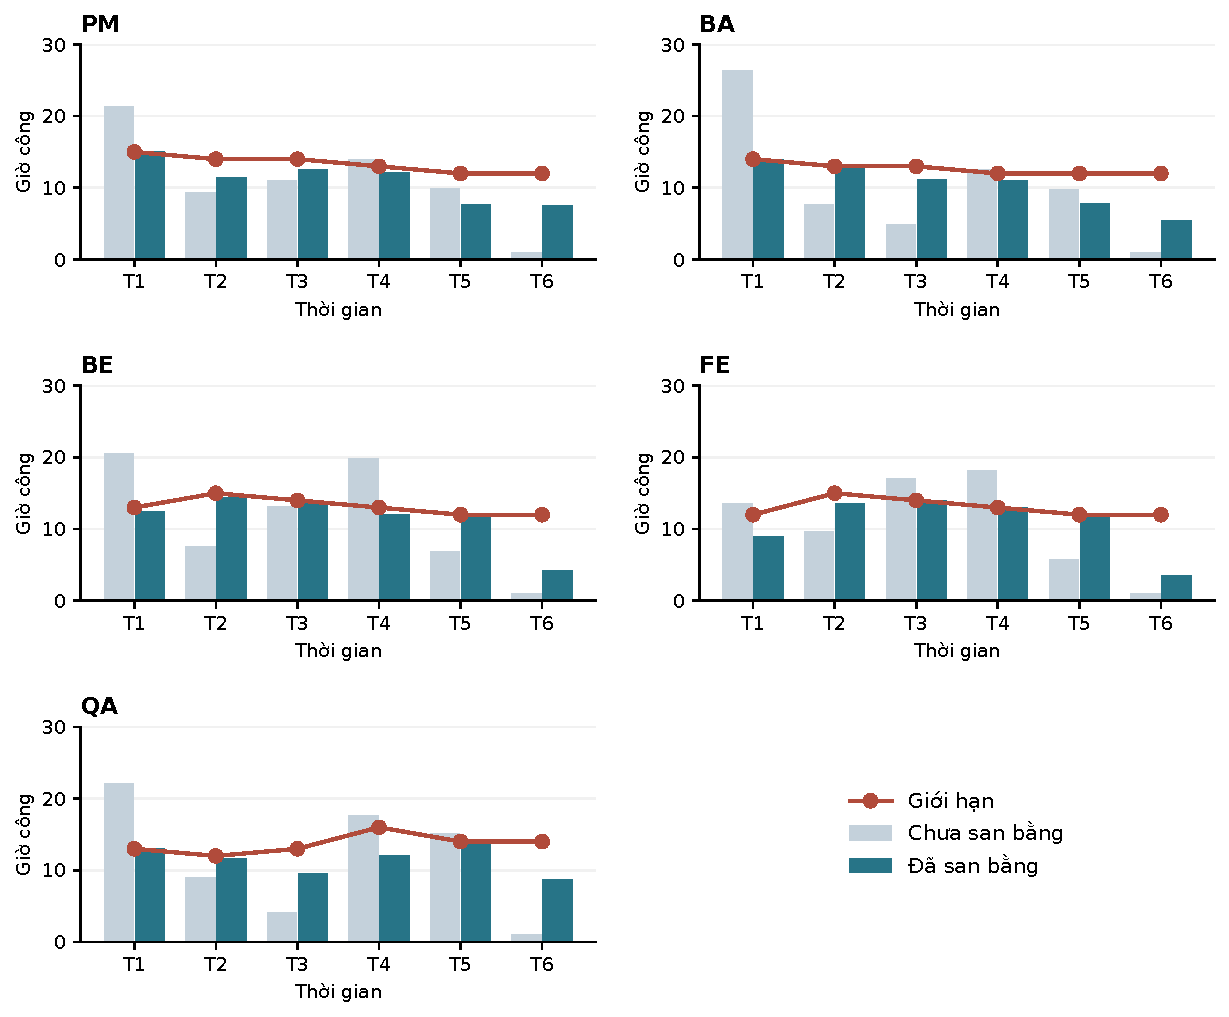
\includegraphics[width=\linewidth]{Images/nguon_luc.pdf}
\caption{Biểu đồ phân bổ Workload nhân sự theo tuần sau Resource Leveling}
\label{fig:resource}
\end{figure}

Kế hoạch phân bổ chính thức ghi nhận dòng công sức theo tuần từ Tuần 1 đến Tuần 6 lần lượt là: 63,5; 64,0; 61,1; 60,2; 53,4 và 29,4 giờ công. Hình \ref{fig:resource} minh họa tính hợp lệ của lịch trình khi toàn bộ cột Workload thực tế đều nằm trong giới hạn Capacity.

\subsubsection{Đánh giá phương án dời tiến độ}

Nhóm đã thử nghiệm kiểm định kịch bản Nén tiến độ (Schedule Compression): "Dồn toàn bộ khối lượng Tuần 6 về Tuần 5" nhằm kết thúc sớm. Kết quả phân tích tại Bảng 47 cho thấy phương án này gây quá tải nghiêm trọng cho tất cả 5 nhân sự.

\begingroup\small
\setlength{\tabcolsep}{5pt}\renewcommand{\arraystretch}{1.15}
\begin{longtable}{@{}lrrrrr@{}}
\caption{Đánh giá Workload khi nén tiến độ Tuần 6 vào Tuần 5 (Đơn vị: Giờ công)}\label{tab:compression}\\
\toprule
\textbf{Nhân sự} & \textbf{Tải T5 gốc} & \textbf{Chuyển từ T6} & \textbf{Total Workload T5} & \textbf{Capacity T5} & \textbf{Over-allocated} \\
\midrule\endfirsthead
\toprule
\textbf{Nhân sự} & \textbf{Tải T5 gốc} & \textbf{Chuyển từ T6} & \textbf{Total Workload T5} & \textbf{Capacity T5} & \textbf{Over-allocated} \\
\midrule\endhead
\bottomrule\endlastfoot
PM & 7,7 & 7,5 & 15,2 & 12,0 & 3,2 \\
BA & 7,8 & 5,5 & 13,3 & 12,0 & 1,3 \\
BE & 12,0 & 4,2 & 16,2 & 12,0 & 4,2 \\
FE & 11,9 & 3,5 & 15,4 & 12,0 & 3,4 \\
QA & 14,0 & 8,7 & 22,7 & 14,0 & 8,7 \\
\end{longtable}\endgroup

Do các tác vụ sau nghiệm thu A12.2 (ngày 30/11) như BL2, A16, A18.2 và A17 đòi hỏi trình tự thực hiện nối tiếp, việc giữ 29,4 giờ công sang Tuần 6 là giải pháp tối ưu, đảm bảo hoàn tất đóng gói hồ sơ và bàn giao sản phẩm chính thức vào ngày 03/12/2026.

\begingroup\small
\setlength{\tabcolsep}{4pt}\renewcommand{\arraystretch}{1.15}
\begin{longtable}{@{}lr@{}}
\caption{Các mốc hoàn thành công việc chính}\label{tab:revised-milestones}\\
\toprule
\textbf{Hạng mục công việc} & \textbf{Ngày hoàn thành kế hoạch} \\
\midrule\endfirsthead
\toprule
\textbf{Hạng mục công việc} & \textbf{Ngày hoàn thành kế hoạch} \\
\midrule\endhead
\midrule\multicolumn{2}{r}{\textit{Còn tiếp}}\\\endfoot
\bottomrule\endlastfoot
Kiểm thử \& sửa lỗi Increment 1 (A06) & 09/11/2026 \\
Kiểm thử \& sửa lỗi Increment 2 (A08) & 19/11/2026 \\
Kiểm thử nghiệm thu Increment 3 (A12.2) & 30/11/2026 \\
Chốt phiên bản \& xác minh User Guide (BL2) & 01/12/2026 \\
Chốt báo cáo quản lý dự án (A18.2) & 02/12/2026 \\
Demo \& Bàn giao sản phẩm chính thức (A17) & 03/12/2026 \\
\end{longtable}\endgroup

\subsubsection{Quản lý Schedule Buffer}

Tổng Capacity khả dụng của nhóm trong 6 tuần là 395,0 giờ công. Chênh lệch 63,4 giờ công giữa Capacity và Baseline ($395{,}0 - 331{,}6$) đóng vai trò là quỹ nguồn lực dự phòng cho các công việc phát sinh.

Khoảng thời gian từ ngày \textbf{04/12 đến 06/12/2026} được thiết lập làm \textbf{Schedule Buffer} (khoảng đệm tiến độ). Khoảng thời gian này dùng để xử lý các yêu cầu chỉnh sửa hoặc hoàn thiện tài liệu sau buổi demo/bàn giao (CP6 ngày 03/12/2026), đảm bảo dự án nộp báo cáo đúng hạn vào ngày 06/12/2026.
\subsection{Lịch trình thực hiện và đường cơ sở chi phí (Cost Baseline)}
\label{sec:schedule-baseline}
Lịch trình chi tiết và Cost Baseline được xây dựng dựa trên 331,6 giờ công đã cân bằng tại Mục \ref{sec:resource-allocation}, bao gồm đầy đủ các tác vụ ứng phó rủi ro RA01--RA06. Dự án khởi động ngày 26/10/2026, bàn giao ngày 03/12/2026 và kết thúc ngày 06/12/2026.
\subsubsection{Quy ước lập lịch}
Lịch trình tuân thủ các quy tắc sau:
\begin{itemize}
    \item \textbf{Khung thời gian:} Tuần làm việc từ thứ Hai đến Chủ nhật, bao gồm 12 cửa sổ P1/P2 từ thứ Hai đến thứ Bảy.
    \item \textbf{Mối quan hệ tiền nhiệm:} Áp dụng dạng Finish-to-Start (FS) ở phiên tiếp theo.
    \item \textbf{Đồng bộ Milestone:} Milestone CP1 kiểm tra Increment 1 sau khi hoàn thành A06 và RA06.
\end{itemize}
\subsubsection{Lịch thực hiện hoạt động chi tiết}
\begingroup\small
\setlength{\tabcolsep}{4pt}\renewcommand{\arraystretch}{1.15}
\begin{longtable}{@{}p{.075\linewidth}p{.255\linewidth}p{.245\linewidth}>{\raggedleft\arraybackslash}p{.06\linewidth}p{.085\linewidth}p{.085\linewidth}@{}}
\caption{Lịch thực hiện chi tiết các hoạt động dự án}\label{tab:dates}\\
\toprule
\textbf{Mã} & \textbf{Hoạt động} & \textbf{Tiền nhiệm} & \textbf{Giờ} & \textbf{Bắt đầu} & \textbf{Kết thúc} \\
\midrule\endfirsthead
\toprule
\textbf{Mã} & \textbf{Hoạt động} & \textbf{Tiền nhiệm} & \textbf{Giờ} & \textbf{Bắt đầu} & \textbf{Kết thúc} \\
\midrule\endhead
\midrule\multicolumn{6}{r}{\textit{Còn tiếp}}\\\endfoot
\bottomrule\endlastfoot
A01 & Thiết kế CSDL, giao diện, API & --- & 16,0 & 26/10 & 28/10 \\
A02.1 & Test case Increment 1 & --- & 5,0 & 27/10 & 02/11 \\
A02.2 & Test case Increment 2 & A01 & 3,5 & 02/11 & 10/11 \\
A02.3 & Test case Increment 3 & A01 & 3,5 & 28/10 & 10/11 \\
A03 & Thiết lập môi trường triển khai & G04, A01 & 8,0 & 29/10 & 30/10 \\
A04.1 & Dữ liệu thử Increment 1 & A01, A02.1 & 3,5 & 03/11 & 03/11 \\
A05.1 & Lập trình Tài khoản, phân quyền & A03 & 18,0 & 02/11 & 04/11 \\
A05.2 & Lập trình Quản lý sự kiện & A03 & 18,0 & 30/10 & 03/11 \\
A06 & Kiểm thử, sửa lỗi Increment 1 & A05.1, A05.2, A04.1, A02.1 & 10,0 & 05/11 & 09/11 \\
A07.1 & Lập trình Đăng ký, hủy, sức chứa & A06, RA06 & 22,0 & 09/11 & 11/11 \\
A07.2 & Lập trình Danh sách chờ FIFO & A07.1, RA01 & 14,0 & 12/11 & 16/11 \\
A07.3 & Lập trình Email thông báo & A07.2, RA03 & 6,0 & 17/11 & 17/11 \\
A08 & Kiểm thử, sửa lỗi Increment 2 & A07.3, A02.2, BL1 & 13,0 & 18/11 & 19/11 \\
A09.1 & Lập trình Điểm danh QR & A08, RA04 & 12,0 & 21/11 & 24/11 \\
A09.2 & Lập trình Điểm danh thủ công & A08 & 10,0 & 20/11 & 23/11 \\
A10.1 & Lập trình Báo cáo cơ bản & A08 & 13,0 & 20/11 & 21/11 \\
A10.2 & Lập trình Xuất CSV/Excel & A10.1 & 5,0 & 23/11 & 23/11 \\
A11 & Tích hợp, triển khai nghiệm thu & A09.1, A09.2, A10.2, RA02 & 7,0 & 24/11 & 25/11 \\
A12.1 & Integration Test & A11, A02.3, BL1 & 14,0 & 26/11 & 27/11 \\
A12.2 & Đo chỉ tiêu, chốt Evidence & A12.1, RA05 & 8,0 & 27/11 & 30/11 \\
A14.1 & Soạn thảo User Guide & A11 & 3,0 & 25/11 & 30/11 \\
A15.1 & Tổng hợp số liệu đánh giá & A08 & 2,0 & 20/11 & 20/11 \\
A15.2 & Chốt đánh giá và bài học & A12.2, G07, A15.1 & 6,0 & 30/11 & 30/11 \\
A16 & Kế hoạch đóng và bàn giao & BL2, A15.2 & 5,0 & 01/12 & 01/12 \\
A17 & Demo và bàn giao sản phẩm & A18.2 & 5,0 & 03/12 & 03/12 \\
A18.1 & Tổng hợp bản thảo báo cáo & G07 & 2,5 & 10/11 & 10/11 \\
A18.2 & Chốt báo cáo quản lý dự án & A16, A19.2, A18.1 & 4,5 & 02/12 & 02/12 \\
A19.1 & Ghi nhận đóng góp, chuẩn bị demo & A06 & 2,5 & 17/11 & 21/11 \\
A19.2 & Hoàn thiện Reflection và diễn tập & A12.2, A19.1 & 2,5 & 01/12 & 01/12 \\
BL1 & Dữ liệu thử Increment 2, 3 & A01, A02.2, A02.3 & 3,5 & 11/11 & 11/11 \\
BL2 & Chốt phiên bản, xác minh User Guide & A12.2, A14.1 & 4,0 & 30/11 & 01/12 \\
G02 & Rà soát sản phẩm và phụ thuộc & --- & 10,0 & 26/10 & 26/10 \\
G03 & Ước lượng, lập kế hoạch lịch trình & G02 & 11,0 & 27/10 & 28/10 \\
G04 & Phê duyệt Project Baseline V1.0 & G03 & 4,0 & 29/10 & 29/10 \\
G05 & Theo dõi và kiểm soát tiến độ & Định kỳ sau G04 & 30,0 & 30/10 & 27/11 \\
G06 & Rà soát và kiểm soát rủi ro & Dữ liệu G05 & 7,5 & 31/10 & 28/11 \\
G07 & Phân tích và quản lý thay đổi & G04 & 8,0 & 04/11 & 09/11 \\
RA01 & Thử nghiệm tải đồng thời & A03 & 2,5 & 09/11 & 09/11 \\
RA02 & Thử nghiệm triển khai AWS Lightsail & A05.1 & 2,5 & 05/11 & 05/11 \\
RA03 & Thử nghiệm dịch vụ Email & A03 & 1,0 & 02/11 & 02/11 \\
RA04 & Thử nghiệm sinh, quét mã QR & A01 & 2,0 & 02/11 & 09/11 \\
RA05 & Thử nghiệm hiệu năng báo cáo & A10.1 & 1,9 & 23/11 & 23/11 \\
RA06 & Làm rõ yêu cầu kỹ thuật & A05.2 & 1,2 & 09/11 & 09/11 \\
\end{longtable}\endgroup
\subsubsection{Lịch phân bổ giờ công theo tuần (Effort Time-Phasing)}
Bảng \ref{tab:ledger} thể hiện lịch phân bổ giờ công của từng tác vụ qua 6 tuần. Dữ liệu này phục vụ theo dõi tiến độ và hạch toán chi phí nhân sự theo tuần.
\begin{table}[H]
\centering
\caption{Lịch phân bổ giờ công theo hoạt động và tuần (Đơn vị: Giờ công)}\label{tab:ledger}
\begingroup\footnotesize
\setlength{\tabcolsep}{2pt}\renewcommand{\arraystretch}{1.18}
\begin{minipage}[t]{.46\linewidth}
\vspace{0pt}\centering
\begin{tabular*}{\linewidth}{@{\extracolsep{\fill}}lrrrrrrr@{}}
\toprule
\textbf{Mã} & \textbf{T1} & \textbf{T2} & \textbf{T3} & \textbf{T4} & \textbf{T5} & \textbf{T6} & \textbf{Tổng} \\
\midrule
A01 & 16,0 & 0,0 & 0,0 & 0,0 & 0,0 & 0,0 & 16,0 \\
A02.1 & 2,0 & 3,0 & 0,0 & 0,0 & 0,0 & 0,0 & 5,0 \\
A02.2 & 0,0 & 2,0 & 1,5 & 0,0 & 0,0 & 0,0 & 3,5 \\
A02.3 & 1,5 & 0,0 & 2,0 & 0,0 & 0,0 & 0,0 & 3,5 \\
A03 & 8,0 & 0,0 & 0,0 & 0,0 & 0,0 & 0,0 & 8,0 \\
A04.1 & 0,0 & 3,5 & 0,0 & 0,0 & 0,0 & 0,0 & 3,5 \\
A05.1 & 0,0 & 18,0 & 0,0 & 0,0 & 0,0 & 0,0 & 18,0 \\
A05.2 & 4,0 & 14,0 & 0,0 & 0,0 & 0,0 & 0,0 & 18,0 \\
A06 & 0,0 & 8,0 & 2,0 & 0,0 & 0,0 & 0,0 & 10,0 \\
A07.1 & 0,0 & 0,0 & 22,0 & 0,0 & 0,0 & 0,0 & 22,0 \\
A07.2 & 0,0 & 0,0 & 10,9 & 3,1 & 0,0 & 0,0 & 14,0 \\
A07.3 & 0,0 & 0,0 & 0,0 & 6,0 & 0,0 & 0,0 & 6,0 \\
A08 & 0,0 & 0,0 & 0,0 & 13,0 & 0,0 & 0,0 & 13,0 \\
A09.1 & 0,0 & 0,0 & 0,0 & 4,4 & 7,6 & 0,0 & 12,0 \\
A09.2 & 0,0 & 0,0 & 0,0 & 8,7 & 1,3 & 0,0 & 10,0 \\
A10.1 & 0,0 & 0,0 & 0,0 & 13,0 & 0,0 & 0,0 & 13,0 \\
A10.2 & 0,0 & 0,0 & 0,0 & 0,0 & 5,0 & 0,0 & 5,0 \\
A11 & 0,0 & 0,0 & 0,0 & 0,0 & 7,0 & 0,0 & 7,0 \\
A12.1 & 0,0 & 0,0 & 0,0 & 0,0 & 14,0 & 0,0 & 14,0 \\
A12.2 & 0,0 & 0,0 & 0,0 & 0,0 & 5,8 & 2,2 & 8,0 \\
A14.1 & 0,0 & 0,0 & 0,0 & 0,0 & 2,8 & 0,2 & 3,0 \\
A15.1 & 0,0 & 0,0 & 0,0 & 2,0 & 0,0 & 0,0 & 2,0 \\
\bottomrule
\end{tabular*}
\end{minipage}\hfill
\begin{minipage}[t]{.46\linewidth}
\vspace{0pt}\centering
\begin{tabular*}{\linewidth}{@{\extracolsep{\fill}}lrrrrrrr@{}}
\toprule
\textbf{Mã} & \textbf{T1} & \textbf{T2} & \textbf{T3} & \textbf{T4} & \textbf{T5} & \textbf{T6} & \textbf{Tổng} \\
\midrule
A15.2 & 0,0 & 0,0 & 0,0 & 0,0 & 0,0 & 6,0 & 6,0 \\
A16 & 0,0 & 0,0 & 0,0 & 0,0 & 0,0 & 5,0 & 5,0 \\
A17 & 0,0 & 0,0 & 0,0 & 0,0 & 0,0 & 5,0 & 5,0 \\
A18.1 & 0,0 & 0,0 & 2,5 & 0,0 & 0,0 & 0,0 & 2,5 \\
A18.2 & 0,0 & 0,0 & 0,0 & 0,0 & 0,0 & 4,5 & 4,5 \\
A19.1 & 0,0 & 0,0 & 0,0 & 2,5 & 0,0 & 0,0 & 2,5 \\
A19.2 & 0,0 & 0,0 & 0,0 & 0,0 & 0,0 & 2,5 & 2,5 \\
BL1 & 0,0 & 0,0 & 3,5 & 0,0 & 0,0 & 0,0 & 3,5 \\
BL2 & 0,0 & 0,0 & 0,0 & 0,0 & 0,0 & 4,0 & 4,0 \\
G02 & 10,0 & 0,0 & 0,0 & 0,0 & 0,0 & 0,0 & 10,0 \\
G03 & 11,0 & 0,0 & 0,0 & 0,0 & 0,0 & 0,0 & 11,0 \\
G04 & 4,0 & 0,0 & 0,0 & 0,0 & 0,0 & 0,0 & 4,0 \\
G05 & 6,0 & 6,0 & 6,0 & 6,0 & 6,0 & 0,0 & 30,0 \\
G06 & 1,0 & 1,5 & 1,5 & 1,5 & 2,0 & 0,0 & 7,5 \\
G07 & 0,0 & 3,0 & 5,0 & 0,0 & 0,0 & 0,0 & 8,0 \\
RA01 & 0,0 & 0,0 & 2,5 & 0,0 & 0,0 & 0,0 & 2,5 \\
RA02 & 0,0 & 2,5 & 0,0 & 0,0 & 0,0 & 0,0 & 2,5 \\
RA03 & 0,0 & 1,0 & 0,0 & 0,0 & 0,0 & 0,0 & 1,0 \\
RA04 & 0,0 & 1,5 & 0,5 & 0,0 & 0,0 & 0,0 & 2,0 \\
RA05 & 0,0 & 0,0 & 0,0 & 0,0 & 1,9 & 0,0 & 1,9 \\
RA06 & 0,0 & 0,0 & 1,2 & 0,0 & 0,0 & 0,0 & 1,2 \\
\bottomrule
\end{tabular*}
\end{minipage}
\endgroup
\end{table}

Tổng công sức phân bổ từ T1 đến T6 lần lượt là 63,5; 64,0; 61,1; 60,2; 53,4 và 29,4 giờ công, tương ứng tổng cộng 331,6 giờ công.

\subsubsection{Danh mục Milestones kế hoạch}
\begingroup\small
\setlength{\tabcolsep}{4pt}\renewcommand{\arraystretch}{1.15}
\begin{longtable}{@{}p{.13\linewidth}p{.13\linewidth}p{.10\linewidth}p{.505\linewidth}@{}}
\caption{Danh mục Milestones kế hoạch}\label{tab:milestones}\\
\toprule
\textbf{Milestone} & \textbf{Tác vụ trước} & \textbf{Ngày} & \textbf{Điều kiện nghiệm thu \& Tiêu chí} \\
\midrule\endfirsthead
\toprule
\textbf{Milestone} & \textbf{Tác vụ trước} & \textbf{Ngày} & \textbf{Điều kiện nghiệm thu \& Tiêu chí} \\
\midrule\endhead
\midrule\multicolumn{4}{r}{\textit{Còn tiếp}}\\\endfoot
\bottomrule\endlastfoot
CPD & A01 & 28/10 & Hoàn thành rà soát thiết kế CSDL, UI và API specification. \\
CP0 & G04 & 29/10 & Phê duyệt Project Baseline V1.0. \\
CP1 & A06 & 09/11 & Increment 1 đạt yêu cầu kiểm thử; hoàn thành tác vụ RA06. \\
CP2 & A08 & 19/11 & Increment 2 đạt yêu cầu kiểm thử chức năng và Regression Test. \\
CP3 & A11 & 25/11 & Build tích hợp hoàn tất trên môi trường AWS Lightsail. \\
CP4 & A12.2 & 30/11 & Hoàn thành kiểm thử nghiệm thu, đạt chỉ tiêu và Quality Evidence. \\
CP5 & A18.2 & 02/12 & Rà soát toàn bộ hồ sơ bàn giao và phiên bản phần mềm. \\
CP6 & A17 & 03/12 & Demo và bàn giao sản phẩm chính thức. \\
Hạn nộp & --- & 06/12 & Nộp đầy đủ bộ hồ sơ dự án theo quy định. \\
\end{longtable}\endgroup
\subsubsection{Biểu đồ Gantt}
Lịch trình dự án được trực quan hóa qua các biểu đồ Gantt (Hình \ref{fig:gantt1}, \ref{fig:gantt2} và \ref{fig:ganttra}). Các thanh biểu diễn thời gian thực hiện tác vụ; các tác vụ thuộc Critical Path được đánh dấu nổi bật để tập trung theo dõi.
\begin{figure}[H]
\centering
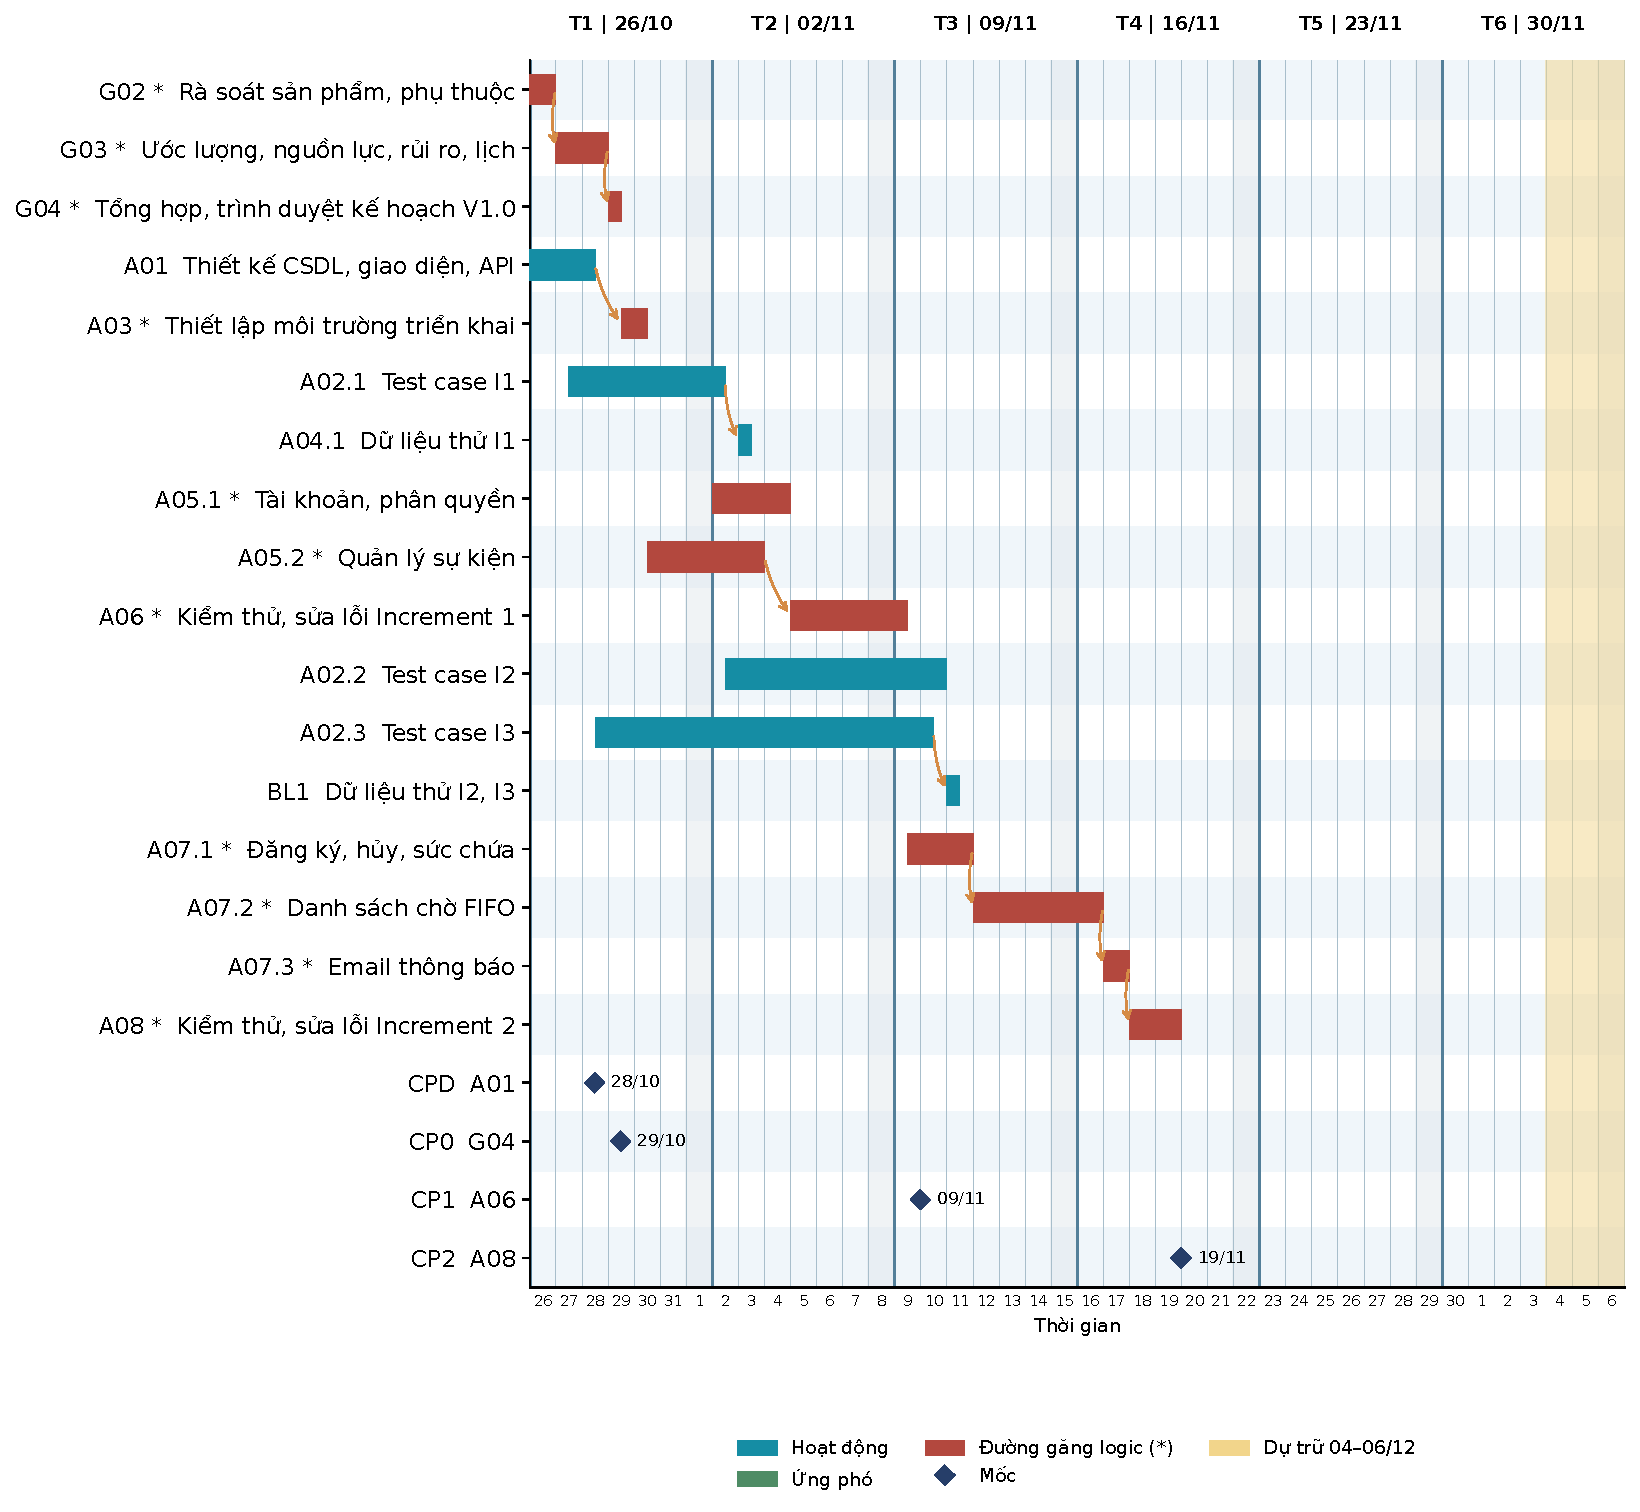
\includegraphics[width=\linewidth,height=.85\textheight,keepaspectratio]{Images/gantt_1.pdf}
\caption{Biểu đồ Gantt tiến độ Increment 1 và Increment 2}
\label{fig:gantt1}
\end{figure}
\begin{figure}[H]
\centering
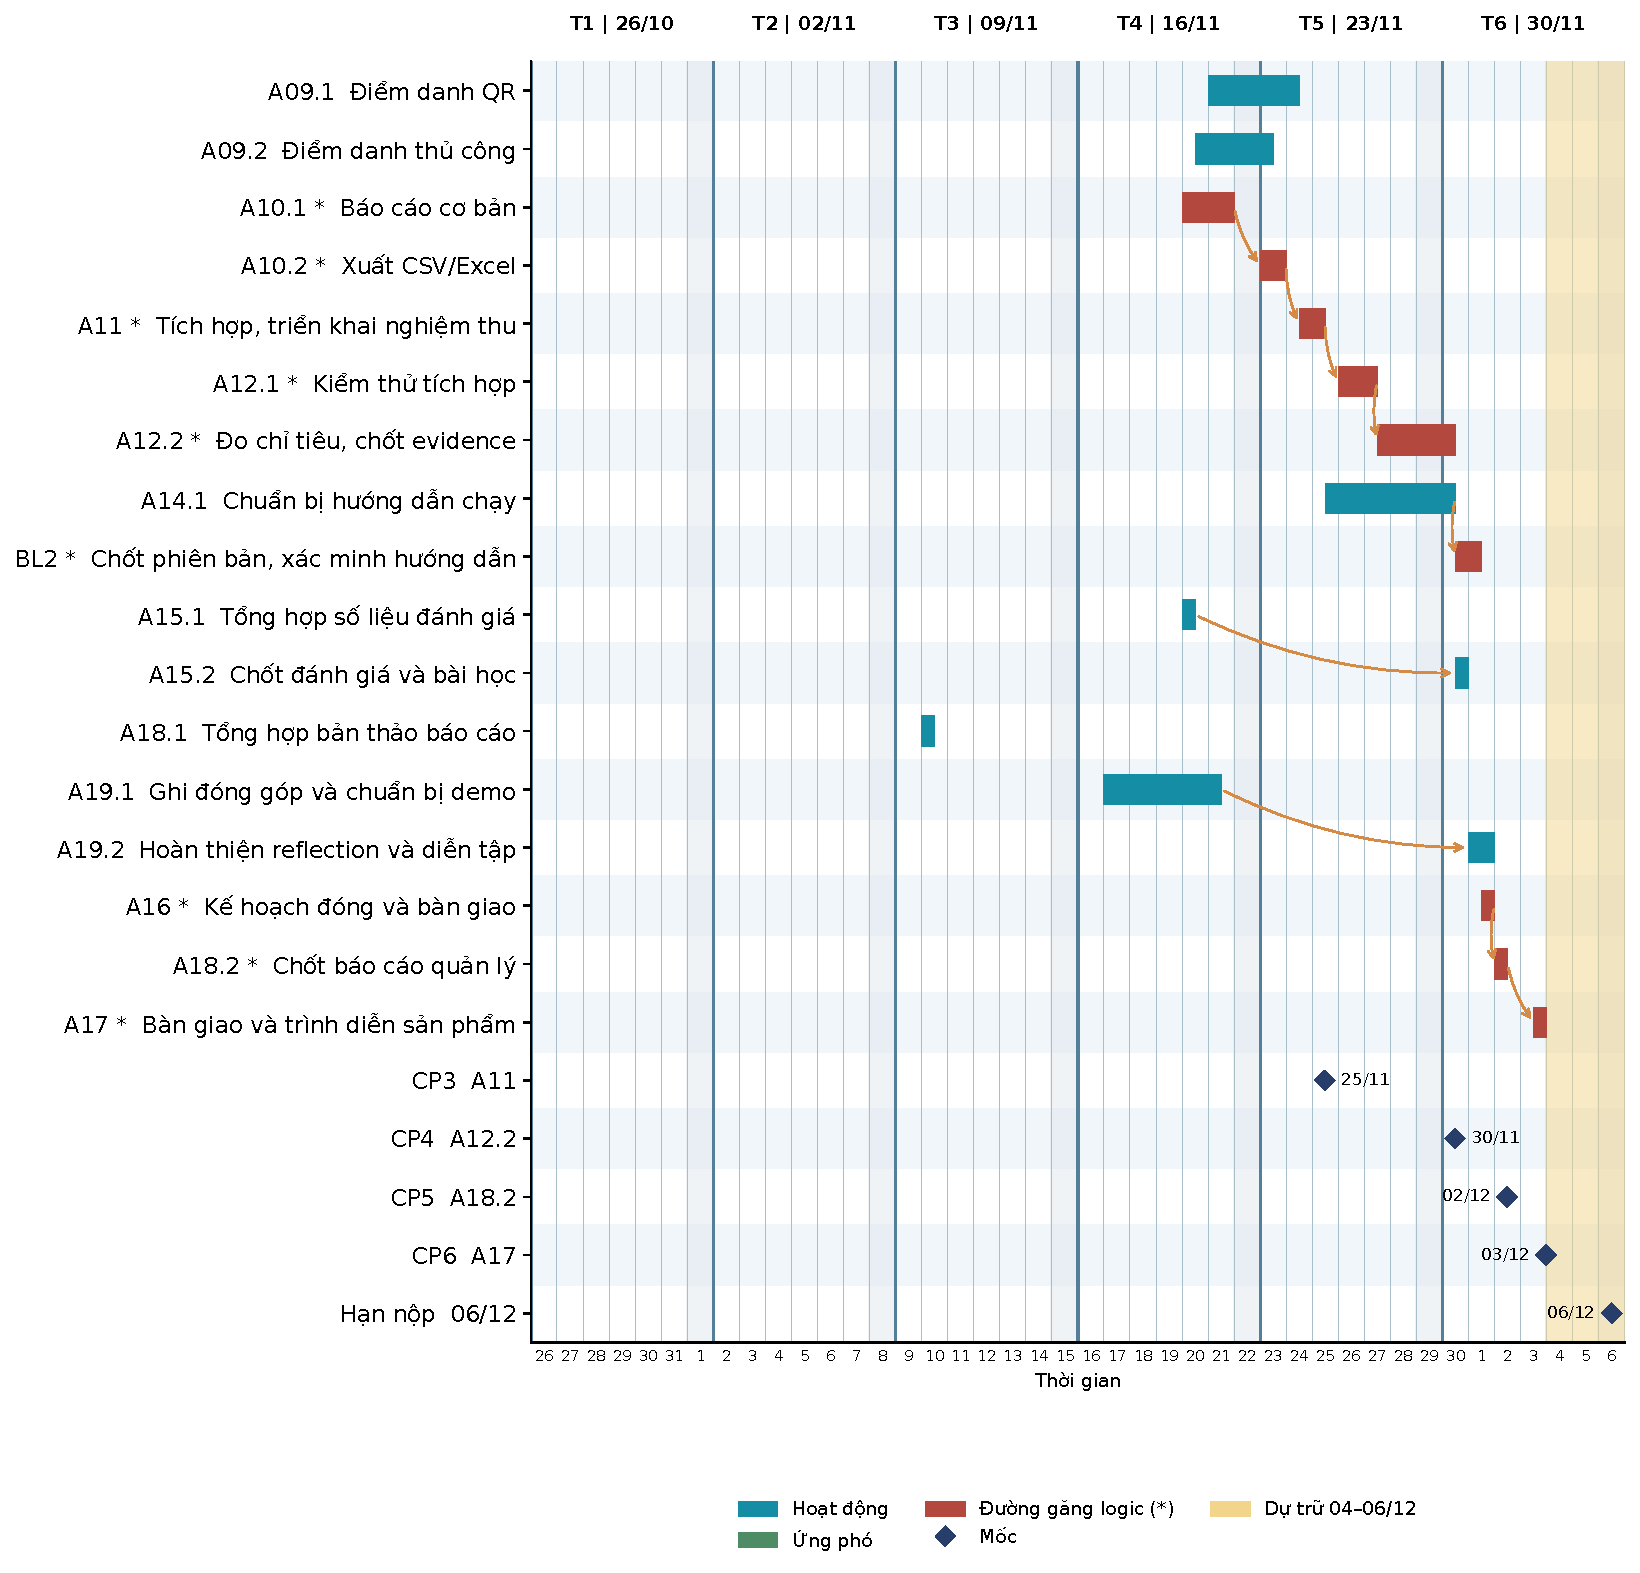
\includegraphics[width=\linewidth,height=.85\textheight,keepaspectratio]{Images/gantt_2.pdf}
\caption{Biểu đồ Gantt tiến độ Increment 3, hoàn thiện hồ sơ và bàn giao}
\label{fig:gantt2}
\end{figure}
\begin{figure}[H]
\centering
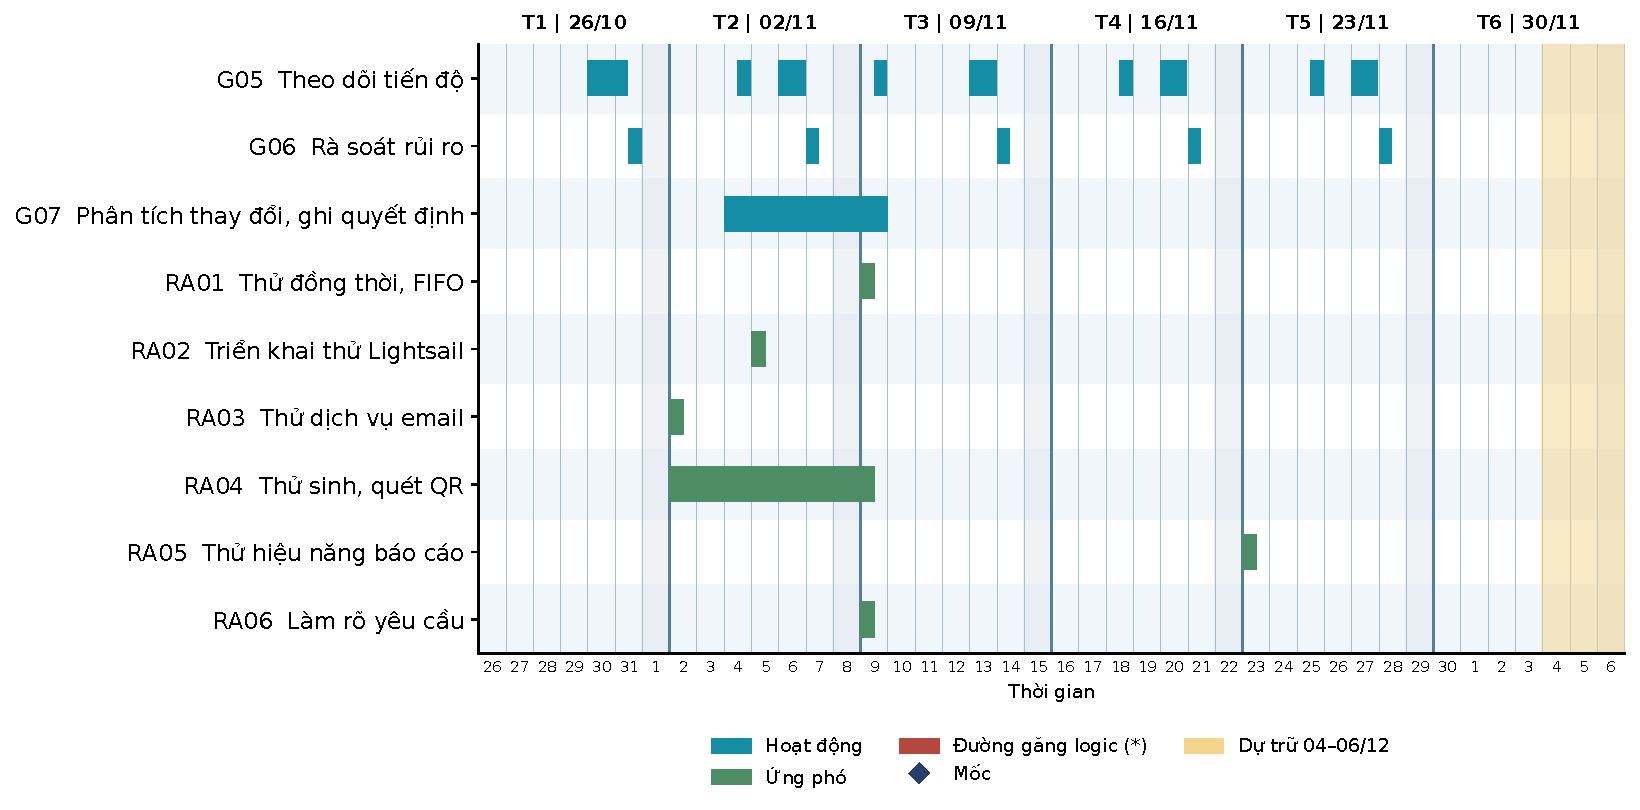
\includegraphics[width=\linewidth]{Images/gantt_ra.pdf}
\caption{Biểu đồ Gantt tiến độ các hoạt động quản lý và tác vụ rủi ro (RA)}
\label{fig:ganttra}
\end{figure}
\subsubsection{Phân tích Critical Path Method (CPM)}
Phương pháp CPM được áp dụng trên sơ đồ mạng công việc sau Activity Splitting. Thời lượng danh định $d_a$ (tính theo phiên) được xác định theo công thức:
\[
d_a=\left\lceil\frac{\max_i e_{a,i}}{2}\right\rceil,
\quad ES_a=\max_{p\in Pred(a)}EF_p,\quad EF_a=ES_a+d_a.
\]
Thuật toán duyệt lùi xác định các tham số $LF, LS$ và Total Float $TF_a = LS_a - ES_a$. Đối với gói BL2, trình tự nội bộ được bảo toàn với $d_{BL2}=2$ phiên.
Kết quả phân tích sơ đồ mạng công việc (Precedence Diagram Method - PDM) cho thấy độ dài Đường găng (Critical Path) là \textbf{47 phiên làm việc}. Chuỗi tác vụ thuộc Critical Path ($TF=0$) gồm:
\begin{quote}\small
G02 $\to$ G03 $\to$ G04 $\to$ A03 $\to$ (A05.1 hoặc A05.2) $\to$ A06 $\to$ A07.1 $\to$ A07.2 $\to$ A07.3 $\to$ A08 $\to$ A10.1 $\to$ A10.2 $\to$ A11 $\to$ A12.1 $\to$ A12.2 $\to$ BL2 $\to$ A16 $\to$ A18.2 $\to$ A17.
\end{quote}
\begin{table}[H]
\centering
\caption{Kết quả tính toán tham số CPM (Đơn vị: Phiên làm việc)}\label{tab:cpm}
\begingroup\footnotesize
\setlength{\tabcolsep}{2pt}\renewcommand{\arraystretch}{1.18}
\begin{minipage}[t]{.46\linewidth}
\vspace{0pt}\centering
\begin{tabular*}{\linewidth}{@{\extracolsep{\fill}}lrrrrrr@{}}
\toprule
\textbf{Mã} & $d$ & $ES$ & $EF$ & $LS$ & $LF$ & $TF$ \\
\midrule
A01 & 4 & 0 & 4 & 2 & 6 & 2 \\
A02.1 & 2 & 0 & 2 & 10 & 12 & 10 \\
A02.2 & 2 & 4 & 6 & 24 & 26 & 20 \\
A02.3 & 2 & 4 & 6 & 24 & 26 & 20 \\
A03 * & 2 & 6 & 8 & 6 & 8 & 0 \\
A04.1 & 1 & 4 & 5 & 12 & 13 & 8 \\
A05.1 * & 5 & 8 & 13 & 8 & 13 & 0 \\
A05.2 * & 5 & 8 & 13 & 8 & 13 & 0 \\
A06 * & 3 & 13 & 16 & 13 & 16 & 0 \\
A07.1 * & 5 & 16 & 21 & 16 & 21 & 0 \\
A07.2 * & 4 & 21 & 25 & 21 & 25 & 0 \\
A07.3 * & 2 & 25 & 27 & 25 & 27 & 0 \\
A08 * & 3 & 27 & 30 & 27 & 30 & 0 \\
A09.1 & 3 & 30 & 33 & 32 & 35 & 2 \\
A09.2 & 2 & 30 & 32 & 33 & 35 & 3 \\
A10.1 * & 3 & 30 & 33 & 30 & 33 & 0 \\
A10.2 * & 2 & 33 & 35 & 33 & 35 & 0 \\
A11 * & 2 & 35 & 37 & 35 & 37 & 0 \\
A12.1 * & 3 & 37 & 40 & 37 & 40 & 0 \\
A12.2 * & 2 & 40 & 42 & 40 & 42 & 0 \\
A14.1 & 1 & 37 & 38 & 41 & 42 & 4 \\
\bottomrule
\end{tabular*}
\end{minipage}\hfill
\begin{minipage}[t]{.46\linewidth}
\vspace{0pt}\centering
\begin{tabular*}{\linewidth}{@{\extracolsep{\fill}}lrrrrrr@{}}
\toprule
\textbf{Mã} & $d$ & $ES$ & $EF$ & $LS$ & $LF$ & $TF$ \\
\midrule
A15.1 & 1 & 30 & 31 & 42 & 43 & 12 \\
A15.2 & 1 & 42 & 43 & 43 & 44 & 1 \\
A16 * & 1 & 44 & 45 & 44 & 45 & 0 \\
A17 * & 1 & 46 & 47 & 46 & 47 & 0 \\
A18.1 & 1 & 8 & 9 & 44 & 45 & 36 \\
A18.2 * & 1 & 45 & 46 & 45 & 46 & 0 \\
A19.1 & 1 & 16 & 17 & 43 & 44 & 27 \\
A19.2 & 1 & 42 & 43 & 44 & 45 & 2 \\
BL1 & 1 & 6 & 7 & 26 & 27 & 20 \\
BL2 * & 2 & 42 & 44 & 42 & 44 & 0 \\
G02 * & 2 & 0 & 2 & 0 & 2 & 0 \\
G03 * & 3 & 2 & 5 & 2 & 5 & 0 \\
G04 * & 1 & 5 & 6 & 5 & 6 & 0 \\
G07 & 2 & 6 & 8 & 41 & 43 & 35 \\
RA01 & 1 & 8 & 9 & 20 & 21 & 12 \\
RA02 & 1 & 13 & 14 & 34 & 35 & 21 \\
RA03 & 1 & 8 & 9 & 24 & 25 & 16 \\
RA04 & 1 & 4 & 5 & 31 & 32 & 27 \\
RA05 & 1 & 33 & 34 & 39 & 40 & 6 \\
RA06 & 1 & 13 & 14 & 15 & 16 & 2 \\
\bottomrule
\end{tabular*}
\end{minipage}
\endgroup
\end{table}
\subsubsection{Đường cơ sở chi phí (Cost Baseline)}
Chi phí nhân sự tính theo đơn giá 78.000 VNĐ/giờ công; chi phí hạ tầng AWS Lightsail cố định 728.000 VNĐ cho hai kỳ thanh toán. Cost Baseline tổng thể ($B$) đã bao gồm 11,1 giờ công RA được xác định là:
\[
B = (331{,}6 \times 78.000) + 728.000 = 25.864.800 + 728.000 = \boxed{26.592.800\text{ VNĐ}}.
\]
\begingroup\small
\setlength{\tabcolsep}{4pt}\renewcommand{\arraystretch}{1.15}
\begin{longtable}{@{}p{.45\linewidth}rr@{}}
\caption{Tổng hợp chi phí theo nhân sự và khoản mục}\label{tab:costtotal}\\
\toprule
\textbf{Khoản mục} & \textbf{Tổng giờ (h)} & \textbf{Chi phí (VNĐ)} \\
\midrule\endfirsthead
\toprule
\textbf{Khoản mục} & \textbf{Tổng giờ (h)} & \textbf{Chi phí (VNĐ)} \\
\midrule\endhead
\midrule\multicolumn{3}{r}{\textit{Còn tiếp}}\\\endfoot
\bottomrule\endlastfoot
PM & 66,4 & 5.179.200 \\
BA & 62,3 & 4.859.400 \\
BE & 68,9 & 5.374.200 \\
FE & 65,0 & 5.070.000 \\
QA & 69,0 & 5.382.000 \\
\textbf{Chi phí công sức nhân sự} & \textbf{331,6} & \textbf{25.864.800} \\
Chi phí hạ tầng AWS Lightsail & --- & 728.000 \\
\textbf{Tổng Cost Baseline} & --- & \textbf{26.592.800} \\
\end{longtable}\endgroup
\begin{table}[H]
\centering
\caption{Phân bổ chi phí công sức theo từng hoạt động}\label{tab:activitycost}
\begingroup\small
\setlength{\tabcolsep}{2pt}\renewcommand{\arraystretch}{1.18}
\begin{minipage}[t]{.46\linewidth}
\vspace{0pt}\centering
\begin{tabular*}{\linewidth}{@{\extracolsep{\fill}}lrr@{}}
\toprule
\textbf{Mã} & \shortstack{\textbf{Công sức}\\\textbf{(h)}} & \shortstack{\textbf{Chi phí}\\\textbf{(VNĐ)}} \\
\midrule
A01 & 16,0 & 1.248.000 \\
A02.1 & 5,0 & 390.000 \\
A02.2 & 3,5 & 273.000 \\
A02.3 & 3,5 & 273.000 \\
A03 & 8,0 & 624.000 \\
A04.1 & 3,5 & 273.000 \\
A05.1 & 18,0 & 1.404.000 \\
A05.2 & 18,0 & 1.404.000 \\
A06 & 10,0 & 780.000 \\
A07.1 & 22,0 & 1.716.000 \\
A07.2 & 14,0 & 1.092.000 \\
A07.3 & 6,0 & 468.000 \\
A08 & 13,0 & 1.014.000 \\
A09.1 & 12,0 & 936.000 \\
A09.2 & 10,0 & 780.000 \\
A10.1 & 13,0 & 1.014.000 \\
A10.2 & 5,0 & 390.000 \\
A11 & 7,0 & 546.000 \\
A12.1 & 14,0 & 1.092.000 \\
A12.2 & 8,0 & 624.000 \\
A14.1 & 3,0 & 234.000 \\
A15.1 & 2,0 & 156.000 \\
\bottomrule
\end{tabular*}
\end{minipage}\hfill
\begin{minipage}[t]{.46\linewidth}
\vspace{0pt}\centering
\begin{tabular*}{\linewidth}{@{\extracolsep{\fill}}lrr@{}}
\toprule
\textbf{Mã} & \shortstack{\textbf{Công sức}\\\textbf{(h)}} & \shortstack{\textbf{Chi phí}\\\textbf{(VNĐ)}} \\
\midrule
A15.2 & 6,0 & 468.000 \\
A16 & 5,0 & 390.000 \\
A17 & 5,0 & 390.000 \\
A18.1 & 2,5 & 195.000 \\
A18.2 & 4,5 & 351.000 \\
A19.1 & 2,5 & 195.000 \\
A19.2 & 2,5 & 195.000 \\
BL1 & 3,5 & 273.000 \\
BL2 & 4,0 & 312.000 \\
G02 & 10,0 & 780.000 \\
G03 & 11,0 & 858.000 \\
G04 & 4,0 & 312.000 \\
G05 & 30,0 & 2.340.000 \\
G06 & 7,5 & 585.000 \\
G07 & 8,0 & 624.000 \\
RA01 & 2,5 & 195.000 \\
RA02 & 2,5 & 195.000 \\
RA03 & 1,0 & 78.000 \\
RA04 & 2,0 & 156.000 \\
RA05 & 1,9 & 148.200 \\
RA06 & 1,2 & 93.600 \\
\bottomrule
\end{tabular*}
\end{minipage}
\endgroup
\end{table}

Tổng công sức của các hoạt động là 331,6 giờ công, tương ứng chi phí nhân sự 25.864.800 VNĐ.

\begingroup\small
\setlength{\tabcolsep}{3pt}\renewcommand{\arraystretch}{1.15}
\begin{longtable}{@{}lrrrrr@{}}
\caption{Bảng phân bổ chi phí kế hoạch theo tuần (Dòng tiền dự án)}\label{tab:weeklycost}\\
\toprule
\textbf{Tuần} & \shortstack{\textbf{Công}\\\textbf{sức (h)}} & \shortstack{\textbf{Chi phí}\\\textbf{nhân sự}} & \shortstack{\textbf{Chi phí}\\\textbf{hạ tầng}} & \shortstack{\textbf{Chi}\\\textbf{phí tuần}} & \shortstack{\textbf{Chi phí}\\\textbf{lũy kế}} \\
\midrule\endfirsthead
\toprule
\textbf{Tuần} & \shortstack{\textbf{Công}\\\textbf{sức (h)}} & \shortstack{\textbf{Chi phí}\\\textbf{nhân sự}} & \shortstack{\textbf{Chi phí}\\\textbf{hạ tầng}} & \shortstack{\textbf{Chi}\\\textbf{phí tuần}} & \shortstack{\textbf{Chi phí}\\\textbf{lũy kế}} \\
\midrule\endhead
\midrule\multicolumn{6}{r}{\textit{Còn tiếp}}\\\endfoot
\bottomrule\endlastfoot
T1 & 63,5 & 4.953.000 & 364.000 & 5.317.000 & 5.317.000 \\
T2 & 64,0 & 4.992.000 & 0 & 4.992.000 & 10.309.000 \\
T3 & 61,1 & 4.765.800 & 0 & 4.765.800 & 15.074.800 \\
T4 & 60,2 & 4.695.600 & 0 & 4.695.600 & 19.770.400 \\
T5 & 53,4 & 4.165.200 & 364.000 & 4.529.200 & 24.299.600 \\
T6 & 29,4 & 2.293.200 & 0 & 2.293.200 & 26.592.800 \\
\textbf{Tổng} & \textbf{331,6} & \textbf{25.864.800} & \textbf{728.000} & \textbf{26.592.800} & --- \\
\end{longtable}\endgroup
\begin{figure}[H]
\centering
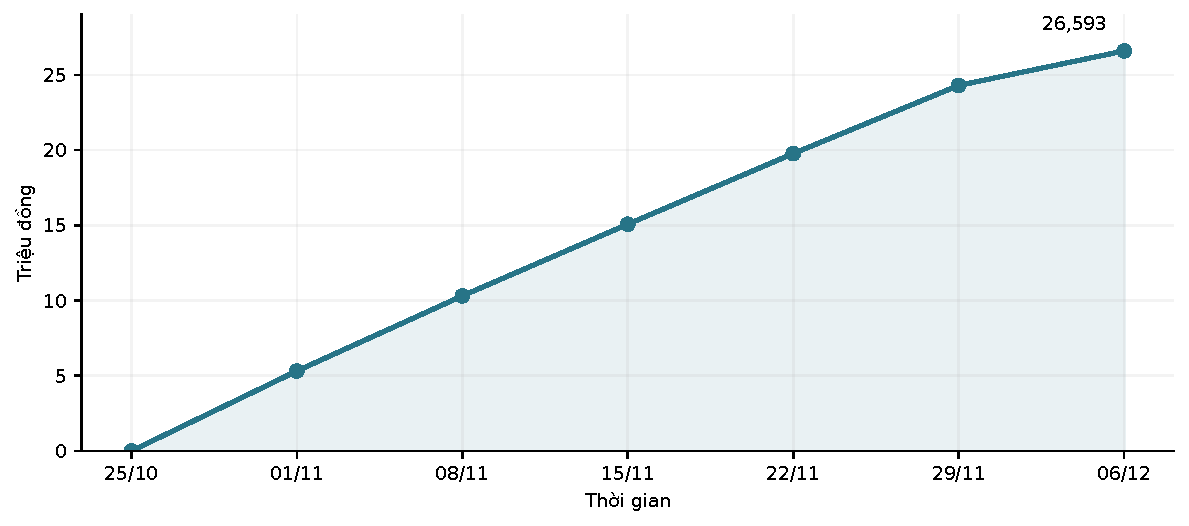
\includegraphics[width=\linewidth]{Images/chi_phi.pdf}
\caption{Đường cong chi phí kế hoạch lũy kế (S-Curve Cost Baseline)}
\label{fig:cost}
\end{figure}
Hình \ref{fig:cost} minh họa S-Curve của Cost Baseline từ mốc 0 VNĐ (ngày 25/10/2026) đạt mốc 26.592.800 VNĐ tại Tuần 6.
\clearpage
\subsection{Rà soát và thiết lập đường cơ sở dự án (Project Baseline)}
\label{sec:baseline-review}

Trước khi phê duyệt Project Baseline V1.0, nhóm dự án tiến hành kiểm tra độc lập tính đầy đủ, tính nhất quán và độ khả thi của toàn bộ hệ thống kế hoạch (gồm Phạm vi, WBS, Rủi ro, Nguồn lực, Lịch trình và Chi phí). Đường cơ sở V1.0 là căn cứ kỹ thuật và quản lý duy nhất để theo dõi tiến độ, kiểm soát chi phí và đánh giá các yêu cầu thay đổi trong suốt quá trình thực thi.

\subsubsection{Rà soát chất lượng kế hoạch}

\begingroup\small
\setlength{\tabcolsep}{4pt}\renewcommand{\arraystretch}{1.15}
\begin{longtable}{@{}p{.22\linewidth}p{.70\linewidth}@{}}
\caption{Nội dung đánh giá chất lượng trước khi phê duyệt Project Baseline}\label{tab:review}\\
\toprule
\textbf{Hạng mục rà soát} & \textbf{Kết quả đánh giá \& Yêu cầu xác minh} \\
\midrule\endfirsthead
\toprule
\textbf{Hạng mục rà soát} & \textbf{Kết quả đánh giá \& Yêu cầu xác minh} \\
\midrule\endhead
\midrule\multicolumn{2}{r}{\textit{Còn tiếp}}\\\endfoot
\bottomrule\endlastfoot
Phạm vi (Scope) & Toàn bộ công việc sau Activity Splitting đều ánh xạ $1-1$ về WBS gốc; các tác vụ ứng phó rủi ro (RA) xác định rõ tiêu chí nghiệm thu. \\
Công sức (Effort) & Tổng khối lượng 331,6 giờ công phân bổ cân đối theo vai trò: PM (66,4h), BA (62,3h), BE (68,9h), FE (65,0h) và QA (69,0h). \\
Nguồn lực & Bảo toàn tổng Capacity 395,0 giờ công; loại bỏ hoàn toàn tình trạng quá tải nguồn lực ($O_{i,w}=0$) sau san bằng. \\
Lịch trình & Khớp nối chặt chẽ giữa các gói thi công; bảo toàn quỹ thời gian dự phòng (Schedule Buffer) ở cuối dự án. \\
Sơ đồ mạng (CPM) & Sơ đồ PDM xác định độ dài Đường găng (Critical Path) là 47 phiên; tính toán chính xác thời gian dự trữ (Float). \\
Chi phí (Cost) & Tổng ngân sách 26.592.800 VNĐ bao gồm chi phí nhân sự và chi phí hạ tầng AWS Lightsail. \\
Điều kiện vận hành & Thống nhất thời khóa biểu cá nhân, môi trường triển khai và các cột mốc làm việc định kỳ với đại diện khách hàng. \\
\end{longtable}\endgroup

\subsubsection{Thành phần Project Baseline V1.0}

\begingroup\small
\setlength{\tabcolsep}{4pt}\renewcommand{\arraystretch}{1.15}
\begin{longtable}{@{}p{.22\linewidth}p{.70\linewidth}@{}}
\caption{Cấu trúc các thành phần cấu thành Project Baseline V1.0}\label{tab:baseline}\\
\toprule
\textbf{Thành phần Baseline} & \textbf{Giá trị chuẩn hóa} \\
\midrule\endfirsthead
\toprule
\textbf{Thành phần Baseline} & \textbf{Giá trị chuẩn hóa} \\
\midrule\endhead
\midrule\multicolumn{2}{r}{\textit{Còn tiếp}}\\\endfoot
\bottomrule\endlastfoot
Phiên bản & Project Baseline V1.0 (Áp dụng chính thức từ ngày ký phê duyệt). \\
Đường cơ sở phạm vi & WBS chi tiết, danh mục Deliverables và tiêu chí nghiệm thu (Mục 2.7--2.9). \\
Đường cơ sở công sức & 331,6 giờ công (320,5h công việc cơ sở + 11,1h tác vụ rủi ro RA). \\
Đường cơ sở lịch trình & Ngày khởi động: 26/10/2026; Bàn giao: 03/12/2026; Hạn nộp báo cáo: 06/12/2026. \\
Đường cơ sở chi phí & 26.592.800 VNĐ (Nhân sự: 25.864.800 VNĐ; Hạ tầng AWS: 728.000 VNĐ). \\
Quỹ dự phòng (Buffer) & Dự phòng nguồn lực: 63,4 giờ công; Schedule Buffer: 04/12--06/12/2026. \\
Hồ sơ đính kèm & Báo cáo kế hoạch, bảng phân bổ, biểu đồ Gantt, ma trận CPM và biên bản rà soát. \\
\end{longtable}\endgroup

\subsubsection{Thống nhất và phê duyệt đường cơ sở}

\begingroup\small
\setlength{\tabcolsep}{4pt}\renewcommand{\arraystretch}{1.15}
\begin{longtable}{@{}p{.20\linewidth}p{.42\linewidth}p{.30\linewidth}@{}}
\caption{Phân công trách nhiệm phê duyệt và bằng chứng xác nhận}\label{tab:agreement}\\
\toprule
\textbf{Bên tham gia} & \textbf{Trách nhiệm phê duyệt} & \textbf{Bằng chứng xác nhận} \\
\midrule\endfirsthead
\toprule
\textbf{Bên tham gia} & \textbf{Trách nhiệm phê duyệt} & \textbf{Bằng chứng xác nhận} \\
\midrule\endhead
\midrule\multicolumn{3}{r}{\textit{Còn tiếp}}\\\endfoot
\bottomrule\endlastfoot
Quản lý dự án (PM) & Rà soát tính logic toàn diện về khối lượng công việc, lịch trình và chi phí. & Biên bản rà soát kế hoạch dự án. \\
Thành viên nhóm & Cam kết phân công công sức, tuân thủ tiến độ và đảm bảo chất lượng. & Xác nhận phê duyệt nội bộ V1.0. \\
Đại diện khách hàng & Phê duyệt Phạm vi, các cột mốc Milestones và tiêu chí nghiệm thu sản phẩm. & Biên bản họp / Email phê duyệt. \\
\end{longtable}\endgroup

\subsubsection{Lưu trữ và kiểm soát phiên bản}
\enlargethispage{3\baselineskip}

Sau khi thu thập đầy đủ phê duyệt, PM tiến hành đóng gói và đóng đếm Project Baseline V1.0 làm mốc tham chiếu duy nhất cho công tác đo lường hiệu quả thực thi trong các giai đoạn tiếp theo. Mọi điều chỉnh về Phạm vi, Lịch trình hay Chi phí phát sinh phải tuân thủ nghiêm ngặt quy trình Quản lý thay đổi (G07) và chỉ có hiệu lực khi ban hành phiên bản Baseline điều chỉnh chính thức (V1.1, V2.0).



\section{Task 3: Software Development, Monitoring \& Control}
\label{sec:execution-i1}

\subsection{Task 3.1. Triển khai phần mềm theo phạm vi đã thống nhất}
\label{sec:t3-implementation}

\subsubsection{Yêu cầu của sản phẩm được triển khai}
\label{sec:t3-requirements}

Mục này chốt phạm vi phần mềm mà Task 3 triển khai. Yêu cầu được rút ra từ phạm vi MVP ở Task 1.4, Client Interaction Log và các quyết định làm rõ trong quá trình thực hiện. Mỗi yêu cầu đã được \textbf{đối chiếu lại với mã nguồn bàn giao} (backend Spring Boot, frontend Angular và tài liệu \texttt{docs/api}) để bảo đảm báo cáo mô tả đúng hệ thống đang chạy, không mô tả theo bản thiết kế ban đầu. Mã FR và NFR được dùng lại trong ma trận truy vết và bằng chứng kiểm thử ở Mục \ref{sec:t3-quality}.

\subsubsubsection{Yêu cầu chức năng (Functional Requirements)}

\begingroup\small
\renewcommand{\arraystretch}{1.15}
\begin{longtable}{@{}p{.08\linewidth}p{.52\linewidth}p{.13\linewidth}p{.17\linewidth}@{}}
\caption{Danh mục yêu cầu chức năng}\label{tab:t3-fr}\\
\toprule
\textbf{Mã} & \textbf{Yêu cầu} & \textbf{Use case} & \textbf{Increment / HĐ}\\\midrule\endfirsthead
\toprule
\textbf{Mã} & \textbf{Yêu cầu} & \textbf{Use case} & \textbf{Increment / HĐ}\\\midrule\endhead
\midrule\multicolumn{4}{r}{\textit{Còn tiếp}}\\\endfoot
\bottomrule\endlastfoot
\multicolumn{4}{@{}l}{\textit{Nhóm 1 -- Tài khoản và phân quyền}}\\
FR-01 & Sinh viên tự tạo tài khoản (họ tên, MSSV, email, khoa, năm học, mật khẩu); vai trò luôn là Sinh viên, MSSV và email không trùng. & UC-01 & I1 / A05.1\\
FR-02 & Đăng nhập bằng email và mật khẩu, đăng xuất, khôi phục phiên khi tải lại trang. & UC-02, UC-03 & I1 / A05.1\\
FR-03 & Đổi mật khẩu; tài khoản dùng mật khẩu tạm bắt buộc đổi trước khi dùng các chức năng khác. & UC-25 & I1 / A05.1\\
FR-04 & Ba vai trò cố định (Sinh viên, Người tổ chức, Quản trị viên); mọi API kiểm tra quyền ở backend; Quản trị viên không mặc nhiên có quyền Người tổ chức. & Tất cả & I1 / A05.1\\
FR-05 & Quản trị viên tìm kiếm tài khoản theo MSSV/email/họ tên, lọc theo vai trò và trạng thái. & UC-21 & I1 / A05.1\\
FR-06 & Quản trị viên cấp tài khoản Người tổ chức với mật khẩu tạm và lý do. & UC-22 & I1 / A05.1\\
FR-07 & Quản trị viên khóa/mở khóa tài khoản có lý do; không tự khóa; luôn còn ít nhất một Quản trị viên đang hoạt động. & UC-23 & I1 / A05.1\\
\multicolumn{4}{@{}l}{\textit{Nhóm 2 -- Sự kiện}}\\
FR-08 & Người tổ chức tạo sự kiện nháp với đủ thông tin: tên, mô tả, địa điểm, đơn vị, 4 mốc thời gian, sức chứa nguyên dương, giới hạn khoa/năm (chọn nhiều). & UC-12 & I1 / A05.2\\
FR-09 & Người tổ chức sửa sự kiện của mình; kiểm tra xung đột phiên bản; chặn thay đổi làm sai đăng ký hiện có. & UC-13 & I1, I2 / A05.2, A07.1\\
FR-10 & Người tổ chức công bố sự kiện nháp hợp lệ; chỉ sự kiện đã công bố mới hiển thị với người dùng khác. & UC-14 & I1 / A05.2\\
FR-11 & Người dùng đã đăng nhập tìm sự kiện đã công bố theo tên (phân trang) và xem chi tiết. & UC-04, UC-05 & I1 / A05.2\\
\multicolumn{4}{@{}l}{\textit{Nhóm 3 -- Đăng ký, danh sách chờ và email}}\\
FR-12 & Sinh viên đủ điều kiện đăng ký trong khung giờ đăng ký; chỉ người \texttt{REGISTERED} chiếm chỗ; không đăng ký trùng. & UC-06 & I2 / A07.1\\
FR-13 & Khi hết chỗ, sinh viên được đưa vào danh sách chờ (\texttt{WAITLISTED}) và biết vị trí của mình. & UC-07 & I2 / A07.2\\
FR-14 & Sinh viên hủy đăng ký hoặc rời danh sách chờ trước giờ bắt đầu; được đăng ký lại trong khung giờ đăng ký. & UC-08 & I2 / A07.1\\
FR-15 & Hệ thống tự đôn người chờ hợp lệ đầu tiên (FIFO) khi có chỗ trống, kể cả sau giờ đóng đăng ký, cho đến giờ bắt đầu. & UC-09 & I2 / A07.2\\
FR-16 & Gửi email khi: đăng ký có chỗ, được đôn từ danh sách chờ, sự kiện đổi địa điểm hoặc thời gian. & UC-06, UC-09, UC-13 & I2 / A07.3\\
FR-17 & Sinh viên xem danh sách sự kiện của mình theo trạng thái và kết quả điểm danh của mình. & UC-10 & I2, I3 / A07.1\\
FR-18 & Người tổ chức xem danh sách đăng ký và danh sách chờ của sự kiện mình phụ trách. & UC-15 & I2 / A07.1\\
\multicolumn{4}{@{}l}{\textit{Nhóm 4 -- Điểm danh, báo cáo và xuất dữ liệu}}\\
FR-19 & Người tổ chức mở/đóng phiên QR có thời hạn 1--30 phút, trong khoảng từ 30 phút trước giờ bắt đầu đến giờ kết thúc. & UC-16 & I3 / A09.1\\
FR-20 & Sinh viên \texttt{REGISTERED} quét QR, xem trước thông tin rồi bấm xác nhận để ghi nhận có mặt; mỗi người một lượt. & UC-11 & I3 / A09.1\\
FR-21 & Người tổ chức ghi nhận hoặc sửa điểm danh thủ công, bắt buộc có lý do; mọi thay đổi được lưu lịch sử. & UC-17, UC-18 & I3 / A09.2\\
FR-22 & Báo cáo theo sự kiện: số đăng ký, chờ, hủy, có mặt, vắng và tỷ lệ tham dự; số vắng chỉ chốt sau giờ kết thúc. & UC-19 & I3 / A10.1\\
FR-23 & Xuất báo cáo và danh sách chi tiết ra tệp CSV đọc được tiếng Việt. & UC-20 & I3 / A10.2\\
\end{longtable}
\endgroup

\subsubsubsection{Yêu cầu phi chức năng (Non-functional Requirements)}

\begingroup\small
\renewcommand{\arraystretch}{1.15}
\begin{longtable}{@{}p{.08\linewidth}p{.14\linewidth}p{.44\linewidth}p{.25\linewidth}@{}}
\caption{Danh mục yêu cầu phi chức năng}\label{tab:t3-nfr}\\
\toprule
\textbf{Mã} & \textbf{Thuộc tính} & \textbf{Yêu cầu đo được} & \textbf{Cách hiện thực / kiểm chứng}\\\midrule\endfirsthead
\toprule
\textbf{Mã} & \textbf{Thuộc tính} & \textbf{Yêu cầu đo được} & \textbf{Cách hiện thực / kiểm chứng}\\\midrule\endhead
\midrule\multicolumn{4}{r}{\textit{Còn tiếp}}\\\endfoot
\bottomrule\endlastfoot
NFR-01 & Hiệu năng & Hiển thị báo cáo $\le$ 5 giây và tạo tệp CSV $\le$ 10 giây với 500 bản ghi đăng ký (chỉ số M2, Task 1.4). & Truy vấn một snapshot; đo trên bộ 2.000 đăng ký (Mục \ref{sec:t3-quality}).\\
NFR-02 & Toàn vẹn dữ liệu & Không vượt sức chứa, không đăng ký trùng, không đôn sai thứ tự khi có nhiều yêu cầu đồng thời; lỗi giữa chừng không để lại dữ liệu dở dang. & Khóa sự kiện trong transaction, \texttt{UNIQUE(event\_id, student\_id)}, rollback toàn bộ; test tranh chấp 6 người/1 chỗ.\\
NFR-03 & Chống ghi đè & Hai người cùng sửa một bản ghi thì người lưu sau nhận lỗi xung đột thay vì ghi đè âm thầm. & Optimistic locking bằng \texttt{version}, trả 409 \texttt{VERSION\_CONFLICT}.\\
NFR-04 & Bảo mật xác thực & Mật khẩu băm BCrypt (cost 12); phiên lưu trong cookie HttpOnly, SameSite=Lax, hết hạn 8 giờ; không lưu token ở localStorage. & \texttt{auth\_sessions} chỉ lưu SHA-256 của token phiên.\\
NFR-05 & Bảo mật ứng dụng & Mọi request ghi có CSRF token; giới hạn tần suất đăng nhập/đăng ký (429); truy cập tài nguyên ngoài quyền trả 404 để không lộ sự tồn tại. & Test RBAC/CSRF ở I1--I3; rate limit kiểm thử bằng unit test và HTTP.\\
NFR-06 & An toàn QR & Mã QR ngẫu nhiên 32 byte, chỉ hợp lệ trong phiên còn hạn; DB không lưu token thô. & Lưu SHA-256 và AES-256-GCM; guard ở database kiểm tra hạn ngay lúc ghi.\\
NFR-07 & Tin cậy email & Lỗi email không làm hỏng thao tác nghiệp vụ; tự thử lại tối đa 5 lần với lỗi tạm thời; không gửi thư cho thao tác đã rollback. & Transactional outbox + Brevo HTTP API.\\
NFR-08 & Riêng tư dữ liệu & Dùng dữ liệu sinh viên giả lập; sinh viên chỉ xem dữ liệu của chính mình; Người tổ chức chỉ xem sự kiện mình phụ trách. & Định danh lấy từ phiên, không nhận \texttt{studentId} từ client.\\
NFR-09 & Khả dụng & Giao diện tiếng Việt, hiển thị giờ Việt Nam (UTC+07:00); dùng được trên điện thoại để quét QR. & Angular responsive; camera cần HTTPS.\\
NFR-10 & Bảo trì & Backend phân tầng Controller--Service--Repository; schema được quản lý bằng migration; có pipeline CI. & Flyway V1/V2; \texttt{.github/workflows/validation.yml}.\\
NFR-11 & Giới hạn tài nguyên & Một lần xuất CSV tối đa 10.000 dòng; vượt quá trả 413, không cắt dữ liệu âm thầm. & Kiểm thử 10.001 dòng bị chặn.\\
NFR-12 & Triển khai & Chạy được trên môi trường cloud qua HTTPS và có hướng dẫn chạy lại ở local bằng Docker Compose. & Vercel + Render + Neon; \texttt{README.md}, \texttt{deploy/}.\\
\end{longtable}
\endgroup

\subsection{Mô hình use case}
\label{sec:t3-usecase}

\subsubsection{Tác nhân}

\begin{table}[H]
\centering\small
\caption{Tác nhân của hệ thống}\label{tab:t3-actors}
\begin{tabularx}{\linewidth}{@{}p{.20\linewidth}X@{}}
\toprule
\textbf{Tác nhân} & \textbf{Vai trò trong hệ thống}\\\midrule
Người dùng & Tác nhân khái quát của ba vai trò bên dưới; chỉ dùng cho đăng nhập, đăng xuất và đổi mật khẩu. Không phải vai trò thứ tư.\\
Sinh viên & Tự tạo tài khoản; tìm, xem, đăng ký, hủy sự kiện; theo dõi sự kiện của mình; quét QR để điểm danh cho chính mình.\\
Người tổ chức & Do Quản trị viên cấp tài khoản; tạo, sửa, công bố sự kiện của mình; xem danh sách đăng ký; mở phiên QR; ghi/sửa điểm danh thủ công; xem báo cáo và xuất CSV.\\
Quản trị viên & Tra cứu tài khoản; cấp tài khoản Người tổ chức; khóa/mở khóa tài khoản. Không có quyền nghiệp vụ của Sinh viên hay Người tổ chức.\\
Dịch vụ email (Brevo) & Hệ thống ngoài nhận yêu cầu gửi thư ở UC-06, UC-09 và UC-13.\\
\bottomrule
\end{tabularx}
\end{table}

\subsubsection{Sơ đồ use case}

\tikzset{
  uc/.style={ellipse, draw, align=center, font=\scriptsize, inner sep=0pt,
             text width=3.9cm},
  ucactor/.pic={
    \draw (0,0.62) circle (0.16);
    \draw (0,0.46) -- (0,0.05) (-0.28,0.33) -- (0.28,0.33)
          (0,0.05) -- (-0.22,-0.35) (0,0.05) -- (0.22,-0.35);
  },
  actorlbl/.style={font=\scriptsize\bfseries, align=center},
  ucext/.style={draw, dashed, -{Stealth[length=2mm]}},
  ucgen/.style={draw, -{Triangle[open, length=3mm, width=3mm]}},
  extlbl/.style={font=\tiny, fill=white, inner sep=1pt},
  sysbox/.style={draw, rounded corners=3pt, thick}
}

Các sơ đồ dưới đây chia theo vai trò để dễ đọc. Đường liền là association; mũi tên nét đứt $\ll$extend$\gg$ hướng từ use case mở rộng tới use case cơ sở; mũi tên tam giác rỗng là generalization. Đăng nhập không được nối $\ll$include$\gg$ tới các use case khác vì đã đăng nhập là tiền điều kiện chung.

\begin{figure}[H]
\centering
\begin{adjustbox}{max width=.82\linewidth}
\begin{tikzpicture}
  \draw[sysbox] (5.4,-0.9) rectangle (11.6,4.0);
  \node[font=\scriptsize\itshape, anchor=north] at (8.5,3.95) {Hệ thống BKevent};
  \node[uc] (u02) at (8.5,2.9) {UC-02\\Đăng nhập};
  \node[uc] (u03) at (8.5,1.5) {UC-03\\Đăng xuất};
  \node[uc] (u24) at (8.5,0.1) {UC-24\\Đổi mật khẩu};
  \pic at (3,1.3) {ucactor};
  \node[actorlbl] at (3,0.6) {Người dùng};
  \coordinate (nd) at (3.35,1.6);
  \foreach \y/\lbl in {3.4/Sinh viên, 1.3/Người tổ chức, -0.8/Quản trị viên} {
    \pic at (0,\y) {ucactor};
    \node[actorlbl] at (0,\y-0.7) {\lbl};
    \draw[ucgen] (0.35,\y+0.3) -- (2.65,1.6);
  }
  \foreach \ucn in {u02,u03,u24} \draw (nd) -- (\ucn.west);
\end{tikzpicture}
\end{adjustbox}
\vspace{8pt}
\caption{Use case tài khoản dùng chung}\label{fig:t3-uc-common}
\end{figure}

\begin{figure}[H]
\centering
\begin{adjustbox}{max width=\linewidth}
\begin{tikzpicture}
  \draw[sysbox] (2.1,1.6) rectangle (14.5,10.1);
  \node[font=\scriptsize\itshape, anchor=north] at (8.3,10.05) {Hệ thống BKevent};
  \node[uc] (u01) at (5.2,9.2) {UC-01\\Đăng ký tài khoản sinh viên};
  \node[uc] (u04) at (5.2,8.05) {UC-04\\Tìm kiếm, xem danh sách sự kiện};
  \node[uc] (u05) at (5.2,6.9) {UC-05\\Xem chi tiết sự kiện};
  \node[uc] (u06) at (5.2,5.75) {UC-06\\Đăng ký tham gia sự kiện};
  \node[uc] (u08) at (5.2,4.6) {UC-08\\Hủy đăng ký / rời danh sách chờ};
  \node[uc] (u10) at (5.2,3.45) {UC-10\\Theo dõi sự kiện của tôi};
  \node[uc] (u11) at (5.2,2.3) {UC-11\\Điểm danh bằng QR};
  \node[uc] (u07) at (11.4,6.9) {UC-07\\Tham gia danh sách chờ};
  \node[uc] (u09) at (11.4,4.6) {UC-09\\Tự động chuyển từ danh sách chờ};
  \draw[ucext] (u07) -- node[extlbl, pos=0.5] {$\ll$extend$\gg$} (u06);
  \draw[ucext] (u09) -- node[extlbl, pos=0.5] {$\ll$extend$\gg$} (u08);
  \pic at (0,5.6) {ucactor};
  \node[actorlbl] at (0,4.9) {Sinh viên};
  \coordinate (sv) at (0.35,5.95);
  \foreach \ucn in {u01,u04,u05,u06,u08,u10,u11} \draw (sv) -- (\ucn.west);
  \pic at (16,4.6) {ucactor};
  \node[actorlbl] at (16,3.9) {Dịch vụ\\email};
  \coordinate (em) at (15.65,4.95);
  \draw (em) -- (u06.east);
  \draw (em) -- (u09.east);
\end{tikzpicture}
\end{adjustbox}
\vspace{8pt}
\caption{Use case của Sinh viên}\label{fig:t3-uc-student}
\end{figure}

\begin{figure}[H]
\centering
\begin{adjustbox}{max width=\linewidth}
\begin{tikzpicture}
  \draw[sysbox] (2.1,0.45) rectangle (14.5,10.1);
  \node[font=\scriptsize\itshape, anchor=north] at (8.3,10.05) {Hệ thống BKevent};
  \node[uc] (u12) at (5.2,9.2) {UC-12\\Tạo sự kiện};
  \node[uc] (u13) at (5.2,8.05) {UC-13\\Cập nhật thông tin sự kiện};
  \node[uc] (u14) at (5.2,6.9) {UC-14\\Công bố sự kiện};
  \node[uc] (u15) at (5.2,5.75) {UC-15\\Xem danh sách đăng ký, chờ};
  \node[uc] (u16) at (5.2,4.6) {UC-16\\Mở/đóng phiên điểm danh QR};
  \node[uc] (u17) at (5.2,3.45) {UC-17\\Ghi nhận điểm danh thủ công};
  \node[uc] (u18) at (5.2,2.3) {UC-18\\Chỉnh sửa kết quả điểm danh};
  \node[uc] (u19) at (5.2,1.15) {UC-19\\Xem báo cáo sự kiện};
  \node[uc] (u09b) at (11.4,6.6) {UC-09\\Tự động chuyển từ danh sách chờ};
  \node[uc] (u20) at (11.4,1.15) {UC-20\\Xuất báo cáo CSV};
  \draw[ucext] (u09b) -- node[extlbl, pos=0.5] {$\ll$extend$\gg$} (u13);
  \draw[ucext] (u20) -- node[extlbl, pos=0.5] {$\ll$extend$\gg$} (u19);
  \pic at (0,4.9) {ucactor};
  \node[actorlbl] at (0,4.2) {Người tổ chức};
  \coordinate (org) at (0.35,5.25);
  \foreach \ucn in {u12,u13,u14,u15,u16,u17,u18,u19} \draw (org) -- (\ucn.west);
  \pic at (16,8.0) {ucactor};
  \node[actorlbl] at (16,7.3) {Dịch vụ\\email};
  \coordinate (em2) at (15.65,8.35);
  \draw (em2) -- (u13.east);
  \draw (em2) -- (u09b.east);
\end{tikzpicture}
\end{adjustbox}
\vspace{8pt}
\caption{Use case của Người tổ chức}\label{fig:t3-uc-organizer}
\end{figure}

\begin{figure}[H]
\centering
\begin{adjustbox}{max width=.62\linewidth}
\begin{tikzpicture}
  \draw[sysbox] (2.1,0.45) rectangle (8.3,4.3);
  \node[font=\scriptsize\itshape, anchor=north] at (5.2,4.25) {Hệ thống BKevent};
  \node[uc] (u21) at (5.2,3.45) {UC-21\\Tra cứu tài khoản};
  \node[uc] (u22) at (5.2,2.3) {UC-22\\Cấp tài khoản người tổ chức};
  \node[uc] (u23) at (5.2,1.15) {UC-23\\Khóa hoặc mở khóa tài khoản};
  \pic at (0,2.0) {ucactor};
  \node[actorlbl] at (0,1.3) {Quản trị viên};
  \coordinate (ad) at (0.35,2.35);
  \foreach \ucn in {u21,u22,u23} \draw (ad) -- (\ucn.west);
\end{tikzpicture}
\end{adjustbox}
\vspace{8pt}
\caption{Use case của Quản trị viên}\label{fig:t3-uc-admin}
\end{figure}

UC-09 không có tác nhân khởi tạo trực tiếp: đây là hành vi tự động trong biên hệ thống, mở rộng có điều kiện của UC-08 (hủy làm trống chỗ) và UC-13 (tăng sức chứa). Ngoài ra, trước khi nhận một đăng ký mới ở UC-06, hệ thống cũng chạy bước đôn để người chờ cũ không bị người đến sau vượt lên.

\subsubsection{Đặc tả use case}

Mỗi use case được đặc tả theo mẫu thống nhất. Các mã lỗi trong luồng ngoại lệ là mã thực tế API trả về, giúp đối chiếu trực tiếp với test case.

\newenvironment{ucspec}[2]{%
  \begingroup\small\renewcommand{\arraystretch}{1.12}%
  \begin{longtable}{@{}>{\bfseries\raggedright\arraybackslash}p{.19\linewidth}>{\raggedright\arraybackslash}p{.77\linewidth}@{}}
  \caption{Đặc tả #1 -- #2}\\
  \toprule
  Use Case ID & #1\\
  Use Case Name & #2\\\midrule
  \endfirsthead
  \toprule\endhead
  \bottomrule\endfoot
}{%
  \end{longtable}\endgroup
}

% ---------------------------------------------------------------- UC-01
\begin{ucspec}{UC-01}{Đăng ký tài khoản sinh viên}
Description & Sinh viên tự tạo tài khoản để dùng hệ thống.\\
Trigger & Sinh viên chọn ``Đăng ký tài khoản''.\\
Primary Actor & Sinh viên (chưa có tài khoản).\\
Secondary Actor & Không có.\\
Pre-condition & Chưa đăng nhập.\\
Post-condition & Thành công: tài khoản vai trò Sinh viên được tạo. Thất bại: không tạo dữ liệu nào.\\
Normal flow & 1.~Sinh viên mở biểu mẫu đăng ký.\newline 2.~Nhập họ tên, MSSV, email, khoa (12 khoa/chương trình), năm học, mật khẩu ($\ge$ 8 ký tự).\newline 3.~Hệ thống chuẩn hóa email (chữ thường) và MSSV (chữ hoa), kiểm tra định dạng và tính duy nhất.\newline 4.~Hệ thống lưu tài khoản với mật khẩu băm BCrypt, vai trò luôn là Sinh viên.\newline 5.~Hệ thống báo thành công và chuyển đến đăng nhập.\\
Alternative flow & 3a.~Thiếu hoặc sai dữ liệu: 400, báo lỗi tại trường tương ứng.\newline 3b.~Email hoặc MSSV đã tồn tại: lỗi email hoặc MSSV đã tồn tại (409), gợi ý đăng nhập.\newline 3c.~Payload chứa vai trò: bị bỏ qua, vẫn tạo Sinh viên.\\
Exception flow & 4a.~Lỗi lưu: rollback toàn bộ, 503.\newline 2a.~Gửi quá nhiều lần: lỗi vượt số lần thử (429), kèm thời gian chờ.\\
\end{ucspec}

% ---------------------------------------------------------------- UC-02
\begin{ucspec}{UC-02}{Đăng nhập}
Description & Xác thực người dùng và mở chức năng theo vai trò.\\
Trigger & Người dùng chọn ``Đăng nhập''.\\
Primary Actor & Người dùng (Sinh viên, Người tổ chức, Quản trị viên).\\
Secondary Actor & Không có.\\
Pre-condition & Có tài khoản; chưa có phiên hợp lệ.\\
Post-condition & Thành công: tạo phiên mới (cookie HttpOnly, hạn 8 giờ). Thất bại: không có phiên.\\
Normal flow & 1.~Người dùng nhập email và mật khẩu.\newline 2.~Hệ thống kiểm tra thông tin và trạng thái \textit{Hoạt động}.\newline 3.~Hệ thống tạo phiên và trả thông tin người dùng.\newline 4.~Giao diện chuyển tới trang làm việc theo vai trò.\\
Alternative flow & 2a.~Sai thông tin hoặc tài khoản bị khóa: cùng một lỗi 401, không cho biết lý do cụ thể.\newline 3a.~Tài khoản đang dùng mật khẩu tạm: chuyển tới UC-24; các API khác trả 403 đến khi đổi.\\
Exception flow & 2b.~Thử sai quá nhiều lần: 429.\newline 2c.~Lỗi dữ liệu: 503, không tạo phiên.\\
\end{ucspec}

% ---------------------------------------------------------------- UC-03
\begin{ucspec}{UC-03}{Đăng xuất}
Description & Kết thúc phiên hiện tại.\\
Trigger & Người dùng chọn ``Đăng xuất''.\\
Primary Actor & Người dùng.\\
Secondary Actor & Không có.\\
Pre-condition & Đang đăng nhập.\\
Post-condition & Phiên bị thu hồi phía máy chủ; cookie bị xóa.\\
Normal flow & 1.~Người dùng chọn đăng xuất.\newline 2.~Hệ thống thu hồi phiên và xóa cookie (204).\newline 3.~Giao diện về màn hình đăng nhập.\\
Alternative flow & 2a.~Phiên đã hết hạn hoặc gọi lại: vẫn trả 204.\\
Exception flow & 2b.~Mất mạng: giao diện xóa người dùng hiện tại, đặt cờ chờ đăng xuất và thử lại khi có mạng; phiên máy chủ tự hết hạn sau tối đa 8 giờ.\\
\end{ucspec}

% ---------------------------------------------------------------- UC-04
\begin{ucspec}{UC-04}{Tìm kiếm và xem danh sách sự kiện}
Description & Tìm các sự kiện đã công bố.\\
Trigger & Người dùng mở trang ``Sự kiện'' hoặc nhập từ khóa.\\
Primary Actor & Sinh viên (người dùng đã đăng nhập khác cũng xem được).\\
Secondary Actor & Không có.\\
Pre-condition & Đã đăng nhập.\\
Post-condition & Hiển thị danh sách; không thay đổi dữ liệu.\\
Normal flow & 1.~Người dùng mở danh sách.\newline 2.~Hệ thống trả các sự kiện \textit{Đã công bố}, sắp theo giờ bắt đầu, 10 sự kiện/trang.\newline 3.~Người dùng nhập từ khóa (tối đa 100 ký tự).\newline 4.~Hệ thống tìm theo tên, không phân biệt hoa thường.\\
Alternative flow & 4a.~Không có kết quả: danh sách rỗng.\newline 2a.~Sự kiện nháp không bao giờ xuất hiện.\\
Exception flow & 4b.~Tham số sai: 400. Lỗi tải: báo lỗi và cho tải lại.\\
\end{ucspec}

% ---------------------------------------------------------------- UC-05
\begin{ucspec}{UC-05}{Xem chi tiết sự kiện}
Description & Xem thông tin, điều kiện tham gia và trạng thái của bản thân.\\
Trigger & Người dùng chọn một sự kiện.\\
Primary Actor & Sinh viên.\\
Secondary Actor & Không có.\\
Pre-condition & Đã đăng nhập; sự kiện đã công bố.\\
Post-condition & Hiển thị chi tiết; không thay đổi dữ liệu.\\
Normal flow & 1.~Hệ thống hiển thị tên, mô tả, địa điểm, đơn vị, các mốc thời gian, sức chứa, giới hạn khoa/năm.\newline 2.~Hệ thống hiển thị số chỗ còn, số người chờ, sinh viên có đủ điều kiện không và trạng thái đăng ký hiện tại.\newline 3.~Nếu đã đăng ký, hiển thị kết quả điểm danh và nút quét QR khi đang trong khung điểm danh.\newline 4.~Sinh viên chọn đăng ký (UC-06), hủy (UC-08) hoặc quay lại.\\
Alternative flow & 2a.~Chưa mở hoặc đã đóng đăng ký: vẫn xem được nhưng nút bị vô hiệu kèm lý do.\newline 2b.~Không thuộc đối tượng: báo ``Không thuộc đối tượng tham gia''.\\
Exception flow & 1a.~Sự kiện không tồn tại hoặc là nháp: lỗi không tìm thấy sự kiện (404).\\
\end{ucspec}

% ---------------------------------------------------------------- UC-06
\begin{ucspec}{UC-06}{Đăng ký tham gia sự kiện}
Description & Ghi nhận sinh viên vào danh sách chính thức khi còn chỗ.\\
Trigger & Sinh viên bấm ``Đăng ký tham gia'' hoặc ``Đăng ký lại''.\\
Primary Actor & Sinh viên.\\
Secondary Actor & Dịch vụ email.\\
Pre-condition & Đã đăng nhập; sự kiện đã công bố; giờ mở $\le$ hiện tại $<$ giờ đóng và trước giờ bắt đầu.\\
Post-condition & Có chỗ: \textit{Đã đăng ký} và yêu cầu email xác nhận được ghi vào outbox. Hết chỗ: tiếp tục UC-07.\\
Normal flow & 1.~Sinh viên bấm đăng ký (định danh lấy từ phiên).\newline 2.~Hệ thống khóa sự kiện, kiểm tra khung giờ và điều kiện khoa AND năm.\newline 3.~Hệ thống đôn người chờ hợp lệ trước (UC-09) rồi kiểm tra chỗ trống.\newline 4.~Hệ thống lưu \textit{Đã đăng ký}, lịch sử và yêu cầu email trong cùng transaction (201).\newline 5.~Sau commit, email xác nhận đăng ký được gửi.\\
Alternative flow & 1a.~Đã \textit{Đã đăng ký}/\textit{Đang chờ}: trả trạng thái hiện có (200), không tạo thêm.\newline 1b.~Đã hủy trước đó: dùng lại dòng đăng ký cũ, tăng version, reset điểm danh về \textit{Chưa ghi nhận} và lưu snapshot cũ.\newline 3a.~Hết chỗ: chuyển sang UC-07.\\
Exception flow & 2a.~Không đủ điều kiện: lỗi không thuộc đối tượng tham gia (403).\newline 2b.~Ngoài khung giờ: lỗi ngoài thời gian đăng ký (409).\newline 4a.~Lỗi ghi: rollback toàn bộ, 503.\newline 5a.~Email lỗi: đăng ký vẫn giữ; outbox thử lại tối đa 5 lần.\\
\end{ucspec}

% ---------------------------------------------------------------- UC-07
\begin{ucspec}{UC-07}{Tham gia danh sách chờ}
Description & Ghi nhận nguyện vọng khi sự kiện đã đủ chỗ.\\
Trigger & Sinh viên bấm ``Tham gia danh sách chờ'' (nút hiển thị khi hết chỗ).\\
Primary Actor & Sinh viên.\\
Secondary Actor & Không có.\\
Pre-condition & Như UC-06; số chỗ còn lại bằng 0.\\
Post-condition & Sinh viên ở trạng thái \textit{Đang chờ}, có thời điểm chờ để xếp FIFO.\\
Normal flow & 1.~Giao diện báo sự kiện đã đủ chỗ và đổi nhãn nút.\newline 2.~Sinh viên bấm nút (đồng ý vào danh sách chờ).\newline 3.~Hệ thống lưu \textit{Đang chờ} với thời điểm vào hàng chờ.\newline 4.~Hệ thống báo vị trí hiện tại trong danh sách chờ.\\
Alternative flow & 2a.~Chỗ vừa trống khi bấm: hệ thống xếp \textit{Đã đăng ký} theo UC-06.\newline 2b.~Chỗ vừa hết khi bấm ``Đăng ký tham gia'': hệ thống đưa vào danh sách chờ và báo vị trí.\\
Exception flow & 3a.~Lỗi ghi: rollback, không cấp vị trí chờ.\newline Không gửi email khi vào danh sách chờ.\\
\end{ucspec}

% ---------------------------------------------------------------- UC-08
\begin{ucspec}{UC-08}{Hủy đăng ký hoặc rời danh sách chờ}
Description & Sinh viên hủy chỗ hoặc rời danh sách chờ trước giờ bắt đầu.\\
Trigger & Sinh viên bấm ``Hủy đăng ký''.\\
Primary Actor & Sinh viên.\\
Secondary Actor & Không có.\\
Pre-condition & Có đăng ký \textit{Đã đăng ký} hoặc \textit{Đang chờ}; chưa đến giờ bắt đầu (kể cả đã đóng đăng ký).\\
Post-condition & Đăng ký chuyển \textit{Đã hủy}; nếu trước đó là \textit{Đã đăng ký}, chỗ được giải phóng và UC-09 chạy.\\
Normal flow & 1.~Sinh viên bấm hủy.\newline 2.~Giao diện hiện hộp xác nhận.\newline 3.~Sinh viên xác nhận; client gửi số phiên bản đang xem.\newline 4.~Hệ thống khóa sự kiện, lưu \textit{Đã hủy} và lịch sử.\newline 5.~Nếu chỗ vừa trống, chạy UC-09 trong cùng transaction.\\
Alternative flow & 2a.~Chọn ``Giữ lại'': không thay đổi.\newline 4a.~Đã hủy rồi: trả hiện trạng (200), không ghi lặp.\newline 4b.~Đã có kết quả có mặt: giữ làm bằng chứng nhưng không tính vào báo cáo.\\
Exception flow & 4c.~Sự kiện đã bắt đầu: lỗi sự kiện đã bắt đầu (409).\newline 4d.~Version cũ: lỗi xung đột phiên bản (409).\newline 4e.~Lỗi ghi: rollback cả hủy và đôn chờ.\\
\end{ucspec}

% ---------------------------------------------------------------- UC-09
\begin{ucspec}{UC-09}{Tự động chuyển từ danh sách chờ}
Description & Tự đôn người chờ hợp lệ đầu tiên khi có chỗ trống.\\
Trigger & Chỗ trống xuất hiện do UC-08, do tăng sức chứa ở UC-13, hoặc trước khi nhận đăng ký mới ở UC-06.\\
Primary Actor & Không có (hành vi tự động trong hệ thống).\\
Secondary Actor & Sinh viên được đôn; Dịch vụ email.\\
Pre-condition & Chưa đến giờ bắt đầu; có chỗ trống và có người \textit{Đang chờ}.\\
Post-condition & Người được chọn thành \textit{Đã đăng ký}, mỗi chỗ chỉ cấp một lần; email thông báo được đôn được ghi vào outbox.\\
Normal flow & 1.~Hệ thống duyệt danh sách chờ theo (thời điểm vào hàng chờ, mã).\newline 2.~Kiểm tra lại điều kiện khoa/năm của người đầu hàng.\newline 3.~Chuyển người hợp lệ sang \textit{Đã đăng ký}, ghi lịch sử.\newline 4.~Lặp lại đến khi hết chỗ hoặc hết người chờ.\newline 5.~Sau commit, gửi email thông báo.\\
Alternative flow & 2a.~Người chờ không còn hợp lệ: ghi \textit{bỏ qua} kèm lý do, vẫn giữ \textit{Đang chờ} và thứ tự cũ để xét lại lần sau.\newline 4a.~Đã qua giờ đóng đăng ký nhưng chưa bắt đầu: vẫn đôn.\\
Exception flow & 1a.~Đã đến giờ bắt đầu: không đôn.\newline 3a.~Lỗi ghi: rollback cùng thao tác kích hoạt.\\
\end{ucspec}

% ---------------------------------------------------------------- UC-10
\begin{ucspec}{UC-10}{Theo dõi sự kiện của tôi}
Description & Sinh viên xem các đăng ký và kết quả tham dự của mình.\\
Trigger & Sinh viên chọn ``Sự kiện của tôi''.\\
Primary Actor & Sinh viên.\\
Secondary Actor & Không có.\\
Pre-condition & Đã đăng nhập.\\
Post-condition & Chỉ hiển thị dữ liệu của chính sinh viên.\\
Normal flow & 1.~Hệ thống liệt kê đăng ký (20/trang) với tên sự kiện, thời gian, địa điểm, trạng thái và vị trí chờ.\newline 2.~Sinh viên lọc theo \textit{Đã đăng ký}/\textit{Đang chờ}/\textit{Đã hủy}.\newline 3.~Sinh viên mở chi tiết để xem kết quả điểm danh (UC-05).\\
Alternative flow & 1a.~Chưa có đăng ký: thông báo và liên kết tìm sự kiện.\newline 3a.~Sự kiện chưa kết thúc và chưa quét: hiển thị ``Chưa ghi nhận'', không kết luận vắng.\\
Exception flow & 1b.~Lỗi tải: báo lỗi và cho tải lại.\\
\end{ucspec}

% ---------------------------------------------------------------- UC-11
\begin{ucspec}{UC-11}{Điểm danh bằng QR}
Description & Sinh viên tự ghi nhận có mặt bằng cách quét QR của phiên.\\
Trigger & Sinh viên chọn ``Quét QR''.\\
Primary Actor & Sinh viên.\\
Secondary Actor & Người tổ chức (đang hiển thị QR, UC-16).\\
Pre-condition & Đã đăng nhập; \textit{Đã đăng ký}; phiên QR còn hiệu lực; thiết bị có camera và truy cập qua HTTPS.\\
Post-condition & Có mặt (\textit{Có mặt}) được lưu với thời gian, phương thức QR và lịch sử.\\
Normal flow & 1.~Sinh viên cấp quyền camera và quét mã.\newline 2.~Hệ thống gọi API preview (chỉ đọc) và hiển thị tên, địa điểm, thời gian sự kiện.\newline 3.~Sinh viên bấm ``Xác nhận''.\newline 4.~Hệ thống kiểm tra lại phiên, token và version của sự kiện, đăng ký, điểm danh.\newline 5.~Hệ thống lưu \textit{Có mặt} và báo thành công.\\
Alternative flow & 2a.~Đã có mặt: hiển thị kết quả cũ, không ghi lặp.\newline 1a.~Không cấp camera: hướng dẫn cấp quyền hoặc nhờ Người tổ chức ghi thủ công (UC-17).\\
Exception flow & 4a.~Phiên đóng, hết hạn hoặc mã sai: lỗi phiên QR không hợp lệ (409).\newline 4b.~Không phải \textit{Đã đăng ký}: lỗi chưa đăng ký chính thức (409).\newline 4c.~Dữ liệu đổi sau preview: lỗi thông tin xác nhận đã cũ (409), phải xem lại và xác nhận mới.\newline 4d.~Ngoài khung điểm danh: lỗi ngoài khung điểm danh (409).\\
\end{ucspec}

% ---------------------------------------------------------------- UC-12
\begin{ucspec}{UC-12}{Tạo sự kiện}
Description & Người tổ chức tạo sự kiện ở trạng thái nháp.\\
Trigger & Người tổ chức chọn ``Tạo sự kiện''.\\
Primary Actor & Người tổ chức.\\
Secondary Actor & Không có.\\
Pre-condition & Đăng nhập vai trò Người tổ chức; đã đổi mật khẩu tạm.\\
Post-condition & Sự kiện \textit{Nháp} thuộc người tạo (lấy từ phiên); chưa hiển thị với người khác.\\
Normal flow & 1.~Nhập tên ($\le$ 250 ký tự), mô tả ($\le$ 20.000 ký tự), địa điểm, đơn vị tổ chức.\newline 2.~Nhập 4 mốc: mở đăng ký $<$ đóng đăng ký $\le$ bắt đầu $<$ kết thúc (giờ UTC+07:00).\newline 3.~Nhập sức chứa nguyên dương; chọn nhiều khoa và nhiều năm học (bỏ trống = tất cả).\newline 4.~Hệ thống kiểm tra và lưu nháp (201).\\
Alternative flow & 4a.~Sai dữ liệu hoặc thứ tự thời gian: 400 kèm lỗi từng trường, giữ nội dung đã nhập.\newline 1a.~Rời trang khi chưa lưu: cảnh báo mất dữ liệu.\\
Exception flow & 4b.~Lỗi lưu: không tạo sự kiện hoặc giới hạn đối tượng dở dang.\\
\end{ucspec}

% ---------------------------------------------------------------- UC-13
\begin{ucspec}{UC-13}{Cập nhật thông tin sự kiện}
Description & Sửa sự kiện nháp hoặc đã công bố có kiểm soát.\\
Trigger & Người tổ chức chọn ``Chỉnh sửa''.\\
Primary Actor & Người tổ chức (chủ sự kiện).\\
Secondary Actor & Dịch vụ email; Sinh viên đã đăng ký hoặc đang chờ.\\
Pre-condition & Sự kiện thuộc người tổ chức hiện tại.\\
Post-condition & Thay đổi được lưu; tăng version; thông báo được tạo nếu là thay đổi quan trọng.\\
Normal flow & 1.~Hệ thống tải dữ liệu và version hiện tại.\newline 2.~Người tổ chức sửa và gửi lưu kèm version.\newline 3.~Hệ thống khóa sự kiện, kiểm tra dữ liệu và ảnh hưởng đến đăng ký.\newline 4.~Hệ thống lưu thay đổi.\newline 5.~Nếu tăng sức chứa và có người chờ: chạy UC-09.\newline 6.~Nếu đổi địa điểm hoặc một trong 4 mốc thời gian: tạo email thông báo thay đổi cho người \textit{Đã đăng ký} và \textit{Đang chờ}.\\
Alternative flow & 6a.~Chỉ sửa tên, mô tả hoặc sức chứa: không gửi email thay đổi.\\
Exception flow & 3a.~Giảm sức chứa dưới số đã đăng ký: lỗi sức chứa nhỏ hơn số đã đăng ký (409).\newline 3b.~Đổi khoa/năm khi đã có người đăng ký: lỗi đổi đối tượng khi đã có người đăng ký (409).\newline 3c.~Version cũ: lỗi xung đột phiên bản (409), không ghi đè.\newline 1a.~Sự kiện của người khác: 404.\\
\end{ucspec}

% ---------------------------------------------------------------- UC-14
\begin{ucspec}{UC-14}{Công bố sự kiện}
Description & Chuyển sự kiện nháp sang công bố.\\
Trigger & Người tổ chức chọn ``Công bố''.\\
Primary Actor & Người tổ chức (chủ sự kiện).\\
Secondary Actor & Không có.\\
Pre-condition & Sự kiện \textit{Nháp} hợp lệ.\\
Post-condition & Sự kiện \textit{Đã công bố}, xuất hiện ở UC-04; đăng ký chỉ mở theo lịch đã đặt.\\
Normal flow & 1.~Giao diện hiện bước xác nhận.\newline 2.~Người tổ chức xác nhận; client gửi version.\newline 3.~Hệ thống kiểm tra nội dung đã lưu và chuyển \textit{Đã công bố}.\\
Alternative flow & 2a.~Hủy: giữ nháp.\newline 3a.~Đã công bố và version khớp: trả hiện trạng, không đổi gì.\\
Exception flow & 3b.~Version cũ: 409. 3c.~Không phải chủ sự kiện: 404.\\
\end{ucspec}

% ---------------------------------------------------------------- UC-15
\begin{ucspec}{UC-15}{Xem danh sách đăng ký và danh sách chờ}
Description & Người tổ chức theo dõi người tham gia sự kiện của mình.\\
Trigger & Người tổ chức mở ``Người tham gia''.\\
Primary Actor & Người tổ chức (chủ sự kiện).\\
Secondary Actor & Không có.\\
Pre-condition & Sự kiện đã công bố và thuộc người tổ chức hiện tại.\\
Post-condition & Hiển thị danh sách; không thay đổi thứ tự chờ.\\
Normal flow & 1.~Hệ thống hiển thị số đã đăng ký, số đang chờ và sức chứa.\newline 2.~Hệ thống liệt kê họ tên, MSSV, email, khoa, năm, trạng thái (20/trang).\newline 3.~Người tổ chức lọc theo trạng thái hoặc tìm trong trang hiện tại.\\
Alternative flow & 2a.~Chưa có ai đăng ký: danh sách rỗng, số liệu bằng 0.\newline 3a.~Cần xuất tệp: dùng UC-20 từ trang báo cáo.\\
Exception flow & 1a.~Không phải chủ sự kiện: 404, không lộ thông tin cá nhân.\\
\end{ucspec}

% ---------------------------------------------------------------- UC-16
\begin{ucspec}{UC-16}{Mở hoặc đóng phiên điểm danh QR}
Description & Người tổ chức kiểm soát thời gian hiệu lực của mã QR.\\
Trigger & Người tổ chức chọn ``Mở điểm danh'' hoặc ``Đóng''.\\
Primary Actor & Người tổ chức (chủ sự kiện).\\
Secondary Actor & Sinh viên quét QR (UC-11).\\
Pre-condition & Sự kiện đã công bố; hiện tại nằm trong khoảng [bắt đầu $-$ 30 phút, kết thúc).\\
Post-condition & Mở: có một phiên với mã QR ngẫu nhiên. Đóng: mã không còn dùng được.\\
Normal flow & 1.~Người tổ chức chọn thời hạn 1--30 phút.\newline 2.~Hệ thống tạo phiên (hạn tối đa đến giờ kết thúc) và hiển thị QR dạng SVG.\newline 3.~Sinh viên quét trong thời hạn phiên.\newline 4.~Người tổ chức đóng phiên khi xong.\\
Alternative flow & 2a.~Đang có phiên còn hạn: trả lại phiên đó, không gia hạn.\newline 2b.~Phiên cũ đã hết hạn: tự đóng và tạo phiên mới.\newline 4a.~Muốn đổi mã: đóng rồi mở phiên mới. Đóng lặp lại không gây lỗi.\\
Exception flow & 2c.~Ngoài khung giờ: lỗi ngoài khung điểm danh (409).\newline 2d.~Backend thiếu khóa mã hóa: lỗi chưa cấu hình khóa mã hóa QR (503).\\
\end{ucspec}

% ---------------------------------------------------------------- UC-17
\begin{ucspec}{UC-17}{Ghi nhận điểm danh thủ công}
Description & Bổ sung có mặt khi sinh viên đến muộn, không quét được QR hoặc mất mạng.\\
Trigger & Người tổ chức chọn ``Ghi có mặt'' cho một sinh viên.\\
Primary Actor & Người tổ chức (chủ sự kiện).\\
Secondary Actor & Sinh viên được xác minh.\\
Pre-condition & Sinh viên \textit{Đã đăng ký}; từ 30 phút trước giờ bắt đầu trở đi (được ghi cả sau giờ kết thúc).\\
Post-condition & Kết quả \textit{Có mặt}, phương thức thủ công, người ghi, lý do và snapshot trước/sau được lưu.\\
Normal flow & 1.~Người tổ chức mở trang điểm danh, tìm sinh viên.\newline 2.~Chọn \textit{Có mặt}, nhập lý do ($\le$ 500 ký tự).\newline 3.~Client gửi version điểm danh (0 nếu chưa có) và version đăng ký.\newline 4.~Hệ thống lưu kết quả và lịch sử trong cùng transaction.\\
Alternative flow & 4a.~Kết quả đã giống hiện trạng: trả hiện trạng, không thêm lịch sử.\newline 1a.~Mất mạng tại sự kiện: ghi tạm ngoài hệ thống, nhập lại khi có mạng kèm lý do.\\
Exception flow & 4b.~Quá sớm: lỗi chưa tới giờ điểm danh (409).\newline 4c.~Version cũ: lỗi xung đột phiên bản (409).\newline 4d.~Không phải \textit{Đã đăng ký}: lỗi chưa đăng ký chính thức (409).\\
\end{ucspec}

% ---------------------------------------------------------------- UC-18
\begin{ucspec}{UC-18}{Chỉnh sửa kết quả điểm danh}
Description & Sửa kết quả điểm danh bị ghi sai.\\
Trigger & Người tổ chức chọn sửa kết quả của một sinh viên.\\
Primary Actor & Người tổ chức (chủ sự kiện).\\
Secondary Actor & Sinh viên có kết quả bị sửa.\\
Pre-condition & Như UC-17; đã có bản ghi điểm danh.\\
Post-condition & Kết quả mới (\textit{Có mặt} hoặc \textit{Chưa ghi nhận}) được lưu; báo cáo dùng kết quả mới ở lần đọc sau.\\
Normal flow & 1.~Người tổ chức xem lịch sử thay đổi của sinh viên.\newline 2.~Chọn kết quả mới và nhập lý do.\newline 3.~Hệ thống kiểm tra hai version và lưu cùng lịch sử (người sửa, thời điểm, trước/sau).\\
Alternative flow & 2a.~Không đổi giá trị: không ghi lịch sử.\\
Exception flow & 3a.~Bản ghi vừa bị sửa hoặc sinh viên vừa hủy/đăng ký lại: 409, phải tải lại.\newline 1a.~Sinh viên hoặc Admin gọi API: 403.\\
\end{ucspec}

% ---------------------------------------------------------------- UC-19
\begin{ucspec}{UC-19}{Xem báo cáo sự kiện}
Description & Tổng hợp số liệu tham dự từ dữ liệu trong hệ thống.\\
Trigger & Người tổ chức mở ``Báo cáo'' và chọn sự kiện.\\
Primary Actor & Người tổ chức (chủ sự kiện).\\
Secondary Actor & Không có.\\
Pre-condition & Sự kiện đã công bố.\\
Post-condition & Hiển thị số liệu và danh sách chi tiết tại cùng một thời điểm đọc.\\
Normal flow & 1.~Hệ thống đếm đăng ký, chờ, hủy, có mặt, chưa ghi nhận.\newline 2.~Tính tỷ lệ = có mặt / \textit{Đã đăng ký} $\times$ 100\%, làm tròn 1 chữ số.\newline 3.~Sau giờ kết thúc: vắng = \textit{Đã đăng ký} chưa có mặt.\newline 4.~Hiển thị tổng quan và danh sách chi tiết có phân trang.\\
Alternative flow & 3a.~Chưa kết thúc: số vắng để trống, ghi rõ là số liệu tạm.\newline 2a.~Không có ai đăng ký: tỷ lệ ``Không áp dụng''.\newline 1a.~Người đã hủy hoặc đang chờ không tính vào mẫu số dù có kết quả cũ.\\
Exception flow & 1b.~Không phải chủ sự kiện: 404. Lỗi truy vấn: không hiển thị số liệu một phần.\\
\end{ucspec}

% ---------------------------------------------------------------- UC-20
\begin{ucspec}{UC-20}{Xuất báo cáo CSV}
Description & Tải báo cáo và danh sách chi tiết dưới dạng tệp CSV.\\
Trigger & Người tổ chức bấm ``Xuất CSV'' trên trang báo cáo.\\
Primary Actor & Người tổ chức (chủ sự kiện).\\
Secondary Actor & Không có.\\
Pre-condition & Đang xem UC-19.\\
Post-condition & Tệp CSV được tải về; dữ liệu gốc không đổi.\\
Normal flow & 1.~Người tổ chức chọn phạm vi (mặc định chỉ \textit{Đã đăng ký}, hoặc tất cả trạng thái).\newline 2.~Hệ thống đọc dữ liệu trong một snapshot.\newline 3.~Hệ thống tạo CSV UTF-8 có BOM, giờ UTC+07:00, tổng quan lặp trên từng dòng chi tiết, chống công thức (ô bắt đầu bằng dấu bằng, dấu cộng, dấu trừ hoặc @).\newline 4.~Trình duyệt tải tệp.\\
Alternative flow & 2a.~Không có người: tệp có một dòng tổng quan, tỷ lệ để trống.\\
Exception flow & 2b.~Vượt 10.000 dòng: lỗi dữ liệu xuất quá lớn (413), không cắt dữ liệu.\\
\end{ucspec}

% ---------------------------------------------------------------- UC-21
\begin{ucspec}{UC-21}{Tra cứu tài khoản}
Description & Quản trị viên tìm tài khoản để hỗ trợ hoặc khóa/mở.\\
Trigger & Quản trị viên mở ``Tài khoản''.\\
Primary Actor & Quản trị viên.\\
Secondary Actor & Không có.\\
Pre-condition & Đăng nhập vai trò Quản trị viên.\\
Post-condition & Hiển thị tài khoản; không hiển thị mật khẩu hoặc token.\\
Normal flow & 1.~Quản trị viên nhập từ khóa (MSSV, email hoặc họ tên).\newline 2.~Chọn lọc vai trò và trạng thái (\textit{Hoạt động}/\textit{Bị khóa}).\newline 3.~Hệ thống trả kết quả có phân trang (20/trang).\newline 4.~Quản trị viên chọn tài khoản để thực hiện UC-23.\\
Alternative flow & 3a.~Không có kết quả: danh sách rỗng.\\
Exception flow & 1a.~Không phải Quản trị viên: 403.\\
\end{ucspec}

% ---------------------------------------------------------------- UC-22
\begin{ucspec}{UC-22}{Cấp tài khoản người tổ chức}
Description & Quản trị viên tạo tài khoản cho người được phân công tổ chức sự kiện.\\
Trigger & Quản trị viên chọn ``Cấp tài khoản người tổ chức''.\\
Primary Actor & Quản trị viên.\\
Secondary Actor & Người tổ chức nhận tài khoản.\\
Pre-condition & Đăng nhập vai trò Quản trị viên.\\
Post-condition & Tài khoản Người tổ chức được tạo với cờ buộc đổi mật khẩu.\\
Normal flow & 1.~Nhập họ tên, email, đơn vị tổ chức, mật khẩu tạm và lý do.\newline 2.~Giao diện hiện bước xác nhận, nhắc đối chiếu người được phân công.\newline 3.~Hệ thống tạo tài khoản (201).\newline 4.~Quản trị viên bàn giao mật khẩu tạm qua kênh riêng (ngoài ứng dụng).\\
Alternative flow & 2a.~Hủy: không tạo.\\
Exception flow & 3a.~Email đã tồn tại: 409, không tạo trùng (không có chuyển vai trò).\newline 3b.~Lỗi ghi: rollback.\\
\end{ucspec}

% ---------------------------------------------------------------- UC-23
\begin{ucspec}{UC-23}{Khóa hoặc mở khóa tài khoản}
Description & Tạm ngừng hoặc khôi phục quyền truy cập của một tài khoản.\\
Trigger & Quản trị viên chọn ``Khóa'' hoặc ``Mở khóa''.\\
Primary Actor & Quản trị viên.\\
Secondary Actor & Chủ tài khoản bị xử lý.\\
Pre-condition & Đã chọn tài khoản qua UC-21.\\
Post-condition & Trạng thái mới được lưu kèm lịch sử; khi khóa, mọi phiên của tài khoản bị thu hồi. Dữ liệu đăng ký và điểm danh được giữ.\\
Normal flow & 1.~Quản trị viên chọn thao tác và nhập lý do.\newline 2.~Hệ thống chạy preview, hiển thị trước/sau và tác động.\newline 3.~Quản trị viên xác nhận.\newline 4.~Hệ thống kiểm tra lại điều kiện và version, lưu trạng thái và thu hồi phiên.\\
Alternative flow & 2a.~Trạng thái không đổi: không ghi lịch sử, không tăng version.\newline 3a.~Hủy: không gửi yêu cầu.\\
Exception flow & 4a.~Tự khóa chính mình hoặc khóa Admin \textit{Hoạt động} cuối cùng: 409.\newline 4b.~Người tổ chức còn sự kiện nháp hoặc chưa kết thúc: lỗi Người tổ chức còn sự kiện đang phụ trách (409).\newline 4c.~Version cũ: lỗi xung đột phiên bản (409).\\
\end{ucspec}

% ---------------------------------------------------------------- UC-24
\begin{ucspec}{UC-24}{Đổi mật khẩu}
Description & Người dùng đổi mật khẩu; bắt buộc với tài khoản dùng mật khẩu tạm.\\
Trigger & Người dùng chọn ``Đổi mật khẩu'' hoặc bị chuyển tới sau khi đăng nhập bằng mật khẩu tạm.\\
Primary Actor & Người dùng.\\
Secondary Actor & Không có.\\
Pre-condition & Đã đăng nhập.\\
Post-condition & Mật khẩu mới được lưu; mọi phiên bị thu hồi; người dùng phải đăng nhập lại.\\
Normal flow & 1.~Nhập mật khẩu hiện tại và mật khẩu mới ($\ge$ 8 ký tự, $\le$ 72 byte).\newline 2.~Hệ thống kiểm tra mật khẩu hiện tại.\newline 3.~Hệ thống lưu mật khẩu mới, xóa cờ mật khẩu tạm, thu hồi các phiên (204).\newline 4.~Giao diện chuyển về đăng nhập.\\
Alternative flow & 2a.~Mật khẩu hiện tại sai: báo lỗi, giữ phiên.\\
Exception flow & 3a.~Lỗi ghi: không đổi mật khẩu, phiên giữ nguyên.\\
\end{ucspec}

\subsection{Tổ chức thực hiện}
\label{sec:i1-organization}

Sau bước lập kế hoạch, quá trình phát triển hệ thống được phân chia thành ba Increment. Increment 1 (I1) thiết lập hạ tầng cốt lõi gồm quản lý tài khoản, phân quyền (RBAC), quản lý sự kiện và tra cứu. Mỗi Increment chỉ được chuyển giao sau khi vượt qua rà soát tại mốc kiểm soát (checkpoint) tương ứng.


Công tác quản lý và vận hành được phân định chặt chẽ theo 5 vai trò:
\begin{itemize}
    \item \textbf{PM:} Theo dõi tiến độ, điều phối nhân sự, quản lý rủi ro và tổng hợp các quyết định phê duyệt.
    \item \textbf{BA:} Trích xuất quy tắc nghiệp vụ, xây dựng tiêu chí nghiệm thu (Acceptance Criteria) và hỗ trợ thiết kế giao diện.
    \item \textbf{BE:} Phụ trách kiến trúc backend, thiết kế CSDL và xây dựng hợp đồng API.
    \item \textbf{FE:} Xây dựng giao diện người dùng Angular, tích hợp API và review phần UI.
    \item \textbf{QA:} Xây dựng kịch bản kiểm thử độc lập, thực thi test suite và theo dõi lỗi phát sinh.
\end{itemize}

Mã nguồn được quản lý theo mô hình Feature Branch và sáp nhập qua Pull Request (PR) có kiểm duyệt chéo. Quá trình kiểm thử độc lập áp dụng phiên bản bộ test và môi trường riêng biệt để bảo đảm tính trung lập. Tiến độ hàng tuần được ghi nhận qua Weekly Project Log (gồm công việc, công sức planned/actual, rủi ro và hành động quản lý). Giờ công thực tế được tổng hợp từ timesheet cá nhân để đối chiếu trực tiếp với các mã hoạt động trong baseline.

\subsection{Chuẩn bị và triển khai Increment 1}
\label{sec:i1-development}

Increment 1 hoàn thiện luồng nghiệp vụ từ khởi tạo tài khoản Organizer đến tạo, công bố và tra cứu sự kiện. Mốc CP1 được thiết lập vào ngày 09/11/2026, ngay sau khi hoàn thành các hoạt động A06 và RA06. Trình tự triển khai bao gồm: cụ thể hóa thiết kế, thiết lập môi trường, phát triển chức năng, kiểm thử và đánh giá checkpoint.

\subsubsection{Chuẩn bị thiết kế}

Kết quả của hoạt động A01 (ERD, đặc tả API, mockup UI) được chuyển đổi thành schema PostgreSQL, hợp đồng REST API và các màn hình Angular thực tế. Nhóm tuân thủ kiến trúc 3 tầng (Controller--Service--Repository), đảm bảo tính toàn vẹn transaction (rollback toàn bộ nếu trùng MSSV hoặc email). API giao tiếp qua định dạng JSON UTF-8 với nhóm mã lỗi chuẩn hóa: 400 (Validation), 401 (Unauthenticated), 403 (Forbidden), 404 (Not Found) và 409 (Conflict). 

Cơ chế xác thực sử dụng Session Cookie HttpOnly kết hợp CSRF token bảo vệ các request ghi (POST/PUT/DELETE). Trên cơ sở đó, nhóm chi tiết hóa backlog I1 thành Lower-level plan nhằm kiểm soát công việc mà không làm thay đổi tổng ngân sách giờ công đã duyệt tại A03, A05.1 và A05.2.

\begin{table}[H]
\centering\small
\caption{Backlog I1}\label{tab:i1-lower}
\begin{tabularx}{\linewidth}{@{}p{.10\linewidth}p{.20\linewidth}XX@{}}
\toprule
\textbf{Gói} & \textbf{Đầu mối kế hoạch} & \textbf{Phần việc chi tiết} & \textbf{Tiêu chí kiểm tra}\\\midrule
A03 & BE; PM, FE, QA & Cấu hình CSDL, biến môi trường, build, API health và hướng dẫn chạy. & Khởi động stack thành công; FE--BE--CSDL kết nối đạt; ghi nhận phần cloud/email còn thiếu.\\
A05.1 & BE; BA hỗ trợ UI & Đăng ký, đăng nhập, session, CSRF, quản trị tài khoản và RBAC. & Luồng hợp lệ vận hành đúng; truy cập trái quyền bị chặn ở API; CSDL nhất quán.\\
A05.2 & PM, FE; BE review & Tạo/sửa/công bố sự kiện; kiểm tra ownership/version; tra cứu danh sách và chi tiết. & Không lộ sự kiện nháp; chặn sửa sự kiện người khác; xử lý xung đột; UI dùng API thật.\\
A06 & QA; Dev sửa lỗi & Chạy test API/UI, phân loại kết quả, xử lý lỗi, retest và chuẩn bị CP1. & Có test report theo phiên bản; sai lệch được xử lý hoặc có quyết định chấp nhận.\\
\bottomrule
\end{tabularx}
\end{table}

Các quy tắc như vòng đời CSRF Token, ngắt session khi logout hoặc cơ chế Optimistic Locking được cập nhật bổ sung vào kế hoạch chi tiết trong quá trình thực hiện. Đây là các chi tiết kỹ thuật thuộc phạm vi đã duyệt, không phải phát sinh yêu cầu mới.

\subsubsection{Thiết lập môi trường}

Môi trường local chạy qua Docker Compose gồm Angular v21.0.0, Spring Boot v3.5.7 (Java 21) và PostgreSQL v17 (schema \texttt{campus}). Ngân sách kế hoạch A03 (8,0h) phân bổ cho PM (2,0h), BE (3,0h), FE (1,0h) và QA (2,0h). Smoke test ngày 03/11 xác nhận hạ tầng kết nối ổn định với schema 15 bảng. Các sự cố socket Docker Desktop, Java socket trên Windows và múi giờ JDBC đã được xử lý ở local.

\begin{table}[H]
\centering\small
\caption{Kết quả chuẩn bị môi trường I1}\label{tab:i1-env}
\begin{tabularx}{\linewidth}{@{}p{.23\linewidth}XX@{}}
\toprule
\textbf{Hạng mục} & \textbf{Kết quả ghi nhận} & \textbf{Phần việc tiếp theo}\\\midrule
Build và khởi động & Docker Compose hoạt động; frontend và backend build thành công. & Lưu build log theo release phục vụ mốc CP1.\\
Kết nối ứng dụng & Smoke test 03/11 (22:53) đạt kết nối FE--BE--PostgreSQL, schema có 15 bảng. & Kết nối thành công chưa thay thế cho kiểm thử chức năng nghiệp vụ.\\
Múi giờ & Backend và CSDL sử dụng Asia/Ho\_Chi\_Minh (UTC+07:00). & Duy trì cấu hình đồng bộ khi triển khai sang máy chủ khác.\\
Triển khai cloud & Đã có cấu trúc thư mục và hướng dẫn vận hành. & Chưa chạy cloud thực tế; tiếp tục RA02 và theo dõi A11.\\
\bottomrule
\end{tabularx}
\end{table}

Dữ liệu thử nghiệm I1 (A04.1) khởi tạo danh mục khoa/viện, tài khoản mẫu cho 3 vai trò (Student, Organizer, Admin) và các sự kiện mẫu. Script kiểm thử tích hợp sử dụng môi trường Compose độc lập với CSDL tmpfs, cho phép thực thi lặp lại các kịch bản tạo, khóa, sửa và rollback mà không ảnh hưởng đến dữ liệu phát triển local.

\subsubsection{Phát triển tài khoản}

Phân hệ tài khoản (A05.1) hỗ trợ sinh viên tự đăng ký với thông tin cá nhân, MSSV, email, khoa và khóa học. Backend mặc định gán vai trò \texttt{STUDENT}; mọi giá trị vai trò do client tự gửi lên đều bị từ chối. MSSV và email bắt buộc duy nhất (ràng buộc Unique), nếu trùng sẽ trả mã lỗi 409. Khi đăng nhập thành công, hệ thống tạo session và trả cookie HttpOnly. Các thao tác ghi bắt buộc có CSRF token hợp lệ; việc ẩn nút trên UI chỉ mang tính hỗ trợ trải nghiệm. Tự kiểm thử dev xác nhận hệ thống xử lý đúng các trường hợp đăng ký hợp lệ, trùng dữ liệu, tài khoản bị khóa và giữ phiên sau reload.

Chức năng Quản trị và RBAC (A05.1) cho phép Admin tìm kiếm tài khoản, lọc theo vai trò/trạng thái, khởi tạo Organizer (cấp mật khẩu tạm buộc đổi lần đầu) và khóa/mở khóa tài khoản. Backend kiểm tra quyền trực tiếp tại tầng API. Quy tắc bảo vệ hệ thống: từ chối Admin tự khóa chính mình, luôn duy trì tối thiểu một Admin \texttt{ACTIVE} và kiểm tra \texttt{version} để chống ghi đè đồng thời. Dự án đã chốt mô hình một vai trò cố định cho mỗi tài khoản và bỏ chức năng chuyển đổi vai trò (UC-24).

\subsubsection{Phát triển sự kiện}

Phân hệ quản lý sự kiện (A05.2) hỗ trợ Organizer tạo sự kiện ở dạng nháp (\texttt{DRAFT}), chỉnh sửa và công bố (\texttt{PUBLISHED}). Thông tin chủ sở hữu (ownership) trích xuất trực tiếp từ session. Ràng buộc thời gian được kiểm tra chặt chẽ: mở đăng ký $\le$ đóng đăng ký $\le$ bắt đầu $\le$ kết thúc; sức chứa phải là số nguyên dương. Mỗi cập nhật đều kiểm tra \texttt{version} (Optimistic Locking) để tránh xung đột dữ liệu (trả lỗi 409 nếu trùng). Thao tác truy cập sự kiện ngoài quyền sở hữu bị chặn bằng lỗi 404.

API tra cứu sự kiện (Danh sách/Chi tiết) chỉ hiển thị sự kiện đã công bố (\texttt{PUBLISHED}) cho người dùng đã xác thực, hỗ trợ phân trang và tìm kiếm theo tiêu đề (có chống SQL Injection). Màn hình Angular kết nối trực tiếp với API thật qua \texttt{EventApi}; chế độ fixture dữ liệu giả chỉ dùng trong tự kiểm thử giao diện.

\begin{table}[H]
\centering\small
\caption{Trạng thái chức năng I1}\label{tab:i1-scope}
\begin{tabularx}{\linewidth}{@{}p{.18\linewidth}XX@{}}
\toprule
\textbf{Nhóm chức năng} & \textbf{Kết quả triển khai} & \textbf{Điều kiện chấp nhận}\\\midrule
Tài khoản và session & Có API và UI; hoàn thành tự kiểm thử. & Ghép kết quả QA với commit bàn giao; hoàn tất review độc lập.\\
Quản trị và RBAC & Phân quyền 3 vai trò, cấp Organizer, bảo vệ Admin. & Chấp thuận phạm vi vai trò cố định; đóng các sai lệch liên quan.\\
Quản lý sự kiện & Tạo, sửa, công bố, kiểm tra ownership và version. & Xác nhận kết quả regression và demo luồng tích hợp.\\
Tra cứu sự kiện & API và giao diện Angular tìm kiếm/chi tiết. & Đồng bộ README; xác nhận sử dụng API thật khi demo.\\
Chức năng I2/I3 & Đã có schema/placeholder; chưa phát triển nghiệp vụ. & Tiếp tục backlog các Increment sau; không tính vào kết quả I1.\\
\bottomrule
\end{tabularx}
\end{table}

\subsubsection{Kiểm thử I1}

Công tác kiểm thử (A06) được tổ chức thành 2 lớp độc lập:
\begin{enumerate}
    \item \textbf{Dev QA:} Unit test backend vượt qua 17 ca test (6 ca \texttt{EventRulesTest}, 5 ca \texttt{EventServiceTest}, 6 ca \texttt{EventReadServiceTest}).
    \item \textbf{Independent QA:} Sử dụng Playwright/TypeScript kiểm thử tự động API và UI E2E theo mô hình Page Object Model.
\end{enumerate}

Kịch bản kiểm thử bao phủ toàn bộ luồng chính và các trường hợp ngoại lệ (dữ liệu trùng, truy cập trái quyền, vi phạm ownership, xung đột version).

\paragraph{Thiết kế test cases.}
Các test case được chuyển đổi từ Acceptance Criteria (A02.1). Dưới đây là danh mục kịch bản kiểm thử chuẩn hóa:

\begin{table}[H]
\centering\small
\caption{Test cases tài khoản}\label{tab:i1-auth-cases}
\begin{tabularx}{\linewidth}{@{}p{.22\linewidth}XX@{}}
\toprule
\textbf{Mã truy vết} & \textbf{Thao tác kiểm tra} & \textbf{Expected result}\\\midrule
UC01-TC01 / TC-AUTH-API-01 & Đăng ký với email, MSSV chưa tồn tại, thông tin hợp lệ. & HTTP 201; vai trò STUDENT; lưu hồ sơ; không lộ thông tin bí mật.\\
UC01-TC02 / TC-AUTH-API-02, 03 & Đăng ký với email hoặc MSSV đã tồn tại. & HTTP 409; chỉ rõ trường trùng; không tạo dữ liệu dở dang.\\
TC-AUTH-API-04 & Chèn role=ADMIN vào payload tự đăng ký. & Backend giữ nguyên vai trò STUDENT; không tăng quyền từ payload.\\
AUTH-05, 06, 09 & Đăng nhập đúng/sai, tài khoản bị khóa, reload, logout. & Chỉ phiên hợp lệ được truy cập; thu hồi session ngay khi logout/khóa.\\
\bottomrule\end{tabularx}
\end{table}

\begin{table}[H]
\centering\small
\caption{Test cases sự kiện}\label{tab:i1-event-cases}
\begin{tabularx}{\linewidth}{@{}p{.17\linewidth}XX@{}}
\toprule
\textbf{Ca kiểm tra} & \textbf{Pre-condition / thao tác} & \textbf{Expected result}\\\midrule
UC12-TC01 & Organizer tạo sự kiện đủ trường, sức chứa 150. & Lưu trạng thái DRAFT; gắn ownership từ session; không hiện công khai.\\
UC14-TC01 & Đặt đóng đăng ký 09:00, bắt đầu 08:00 cùng ngày. & Từ chối mốc thời gian không hợp lệ; không cho phép công bố.\\
Ownership & Organizer B thao tác trên sự kiện của Organizer A. & HTTP 404; giữ nguyên sự kiện; không tiết lộ tài nguyên ngoài quyền.\\
Version conflict & Hai phiên chỉnh sửa cùng gửi lưu trên 1 version. & Một cập nhật thành công; yêu cầu dùng version cũ nhận lỗi 409.\\
Tra cứu & Tìm kiếm sự kiện PUBLISHED và DRAFT. & Chỉ trả về PUBLISHED; sự kiện DRAFT hoặc ID không tồn tại nhận 404.\\
\bottomrule\end{tabularx}
\end{table}

\begin{table}[H]
\centering\small
\caption{Test cases phân quyền}\label{tab:i1-rbac-cases}
\begin{tabularx}{\linewidth}{@{}p{.20\linewidth}XX@{}}
\toprule
\textbf{Nhóm} & \textbf{Thao tác kiểm tra} & \textbf{Expected result}\\\midrule
RBAC-TC01 / AUTH-08 & Session STUDENT gọi API quản trị \path{/api/admin/users}. & HTTP 403; chặn thao tác; không thay đổi dữ liệu.\\
CSRF / AUTH-07 & Bỏ CSRF token trên request ghi (POST/PUT/DELETE). & Request bị từ chối; dữ liệu không bị ghi nhận.\\
ADM-02, 03 & Admin cấp Organizer; đăng nhập tài khoản mới. & Yêu cầu đổi mật khẩu tạm ở lần đầu; sau đó mới cấp quyền nghiệp vụ.\\
ADM-06, 07 & Admin tự khóa; hai Admin khóa đồng thời. & Chặn tự khóa; luôn duy trì tối thiểu một Admin ACTIVE.\\
ADM-05 & Gọi API đổi vai trò tài khoản (UC-24). & HTTP 403; giữ nguyên vai trò cố định theo thiết kế mới.\\
\bottomrule\end{tabularx}
\end{table}

\paragraph{Đặc tả test cases.}
Các bảng sau mô tả chi tiết năm test case tiêu biểu của I1. Kết quả mong đợi là tiêu chí đối chiếu; kết quả thực thi được ghi nhận riêng trong test report và phần tổng hợp regression.

\begin{table}[H]
\centering
\begingroup\small
\renewcommand{\arraystretch}{1.18}
\caption{Đăng ký tài khoản thành công}\label{tab:i1-detail-1}
\begin{tabularx}{\linewidth}{@{}p{.23\linewidth}>{\raggedright\arraybackslash}X@{}}
\toprule
\textbf{Mã test case} & \textbf{UC01-TC01} \\\midrule
\textbf{Mục tiêu} & Kiểm tra luồng đăng ký tài khoản sinh viên với thông tin hợp lệ. \\ \addlinespace[3pt]
\textbf{Loại kiểm thử} & UI / Functional; tự động hóa bằng Playwright. \\ \addlinespace[3pt]
\textbf{Điều kiện tiên quyết} & Môi trường hoạt động ổn định; email và MSSV dùng kiểm thử chưa tồn tại trong CSDL. \\ \addlinespace[3pt]
\textbf{Dữ liệu} & Họ tên: Sinh Viên Một; MSSV: 9991111; email: sv01.test@example.edu.vn; khoa: Khoa Học Máy Tính; mật khẩu: Test@12345. \\ \addlinespace[3pt]
\textbf{Bước thực hiện} & 1. Mở trang Đăng ký tài khoản.\newline 2. Nhập đầy đủ thông tin hợp lệ.\newline 3. Nhấn Đăng ký.\newline 4. Đăng nhập bằng tài khoản vừa tạo. \\ \addlinespace[3pt]
\textbf{Kết quả mong đợi} & Tài khoản được tạo với vai trò STUDENT; mật khẩu không xuất hiện trong phản hồi. Người dùng có thể đăng nhập bằng thông tin vừa đăng ký. \\ \addlinespace[3pt]
\textbf{Kết quả thực tế} & Đối chiếu test report của lần chạy tương ứng; không dùng kết quả mong đợi để thay cho trạng thái thực thi. \\ \addlinespace[3pt]
\bottomrule
\end{tabularx}
\endgroup
\end{table}

\begin{table}[H]
\centering
\begingroup\small
\renewcommand{\arraystretch}{1.18}
\caption{Đăng ký trùng dữ liệu}\label{tab:i1-detail-2}
\begin{tabularx}{\linewidth}{@{}p{.23\linewidth}>{\raggedright\arraybackslash}X@{}}
\toprule
\textbf{Mã test case} & \textbf{UC01-TC02} \\\midrule
\textbf{Mục tiêu} & Kiểm tra ràng buộc duy nhất của email và MSSV. \\ \addlinespace[3pt]
\textbf{Loại kiểm thử} & API / Validation; tự động hóa bằng Playwright. \\ \addlinespace[3pt]
\textbf{Điều kiện tiên quyết} & Đã có tài khoản với email sv01.test@example.edu.vn và MSSV 9991111. \\ \addlinespace[3pt]
\textbf{Dữ liệu} & Lần 1: email đã tồn tại, MSSV mới. Lần 2: MSSV đã tồn tại, email mới. Các trường khác hợp lệ. \\ \addlinespace[3pt]
\textbf{Bước thực hiện} & 1. Chuẩn bị tài khoản có sẵn.\newline 2. Gửi yêu cầu đăng ký với email trùng.\newline 3. Gửi yêu cầu riêng với MSSV trùng.\newline 4. Kiểm tra phản hồi và dữ liệu sau mỗi yêu cầu. \\ \addlinespace[3pt]
\textbf{Kết quả mong đợi} & API trả HTTP 409 Conflict cho từng trường hợp; không tạo tài khoản mới hoặc bản ghi hồ sơ dở dang. \\ \addlinespace[3pt]
\textbf{Kết quả thực tế} & Đối chiếu test report theo từng trường hợp email trùng và MSSV trùng. \\ \addlinespace[3pt]
\bottomrule
\end{tabularx}
\endgroup
\end{table}

\begin{table}[H]
\centering
\begingroup\small
\renewcommand{\arraystretch}{1.18}
\caption{Tạo sự kiện nháp}\label{tab:i1-detail-3}
\begin{tabularx}{\linewidth}{@{}p{.23\linewidth}>{\raggedright\arraybackslash}X@{}}
\toprule
\textbf{Mã test case} & \textbf{UC12-TC01} \\\midrule
\textbf{Mục tiêu} & Kiểm tra Organizer tạo sự kiện ở trạng thái DRAFT. \\ \addlinespace[3pt]
\textbf{Loại kiểm thử} & UI / Functional; tự động hóa bằng Playwright. \\ \addlinespace[3pt]
\textbf{Điều kiện tiên quyết} & Organizer đã đăng nhập; đã đổi mật khẩu tạm nếu được yêu cầu. Có tài khoản Student để kiểm tra khả năng tra cứu. \\ \addlinespace[3pt]
\textbf{Dữ liệu} & Tên: Hội thảo Demo QA; địa điểm: Hội trường A; sức chứa: 150. Các mốc thời gian hợp lệ: mở đăng ký < đóng đăng ký $\leq$ bắt đầu < kết thúc. \\ \addlinespace[3pt]
\textbf{Bước thực hiện} & 1. Mở chức năng Tạo sự kiện.\newline 2. Nhập đầy đủ thông tin hợp lệ.\newline 3. Lưu nháp.\newline 4. Kiểm tra sự kiện trong danh sách quản lý.\newline 5. Dùng tài khoản Student tra cứu sự kiện. \\ \addlinespace[3pt]
\textbf{Kết quả mong đợi} & Sự kiện được lưu ở trạng thái DRAFT, thuộc Organizer đang đăng nhập. Student không thấy sự kiện trên danh sách công khai; truy cập chi tiết sự kiện chưa công bố nhận HTTP 404. \\ \addlinespace[3pt]
\textbf{Kết quả thực tế} & Đối chiếu test report của ca tạo nháp và kiểm tra khả năng truy cập từ Student. \\ \addlinespace[3pt]
\bottomrule
\end{tabularx}
\endgroup
\end{table}

\begin{table}[H]
\centering
\begingroup\small
\renewcommand{\arraystretch}{1.18}
\caption{Ràng buộc thời gian}\label{tab:i1-detail-4}
\begin{tabularx}{\linewidth}{@{}p{.23\linewidth}>{\raggedright\arraybackslash}X@{}}
\toprule
\textbf{Mã test case} & \textbf{UC14-TC01} \\\midrule
\textbf{Mục tiêu} & Kiểm tra hệ thống từ chối lịch sự kiện có thời điểm đóng đăng ký muộn hơn thời điểm bắt đầu. \\ \addlinespace[3pt]
\textbf{Loại kiểm thử} & API / Validation; tự động hóa bằng Playwright. \\ \addlinespace[3pt]
\textbf{Điều kiện tiên quyết} & Organizer có phiên đăng nhập hợp lệ và sở hữu một sự kiện DRAFT với lịch ban đầu hợp lệ. \\ \addlinespace[3pt]
\textbf{Dữ liệu} & Đóng đăng ký: 20/11/2026 09:00; bắt đầu: 20/11/2026 08:00. Các trường khác giữ hợp lệ. \\ \addlinespace[3pt]
\textbf{Bước thực hiện} & 1. Mở sự kiện nháp của Organizer.\newline 2. Gửi cập nhật với các mốc thời gian trên.\newline 3. Kiểm tra phản hồi và dữ liệu đã lưu.\newline 4. Kiểm tra trạng thái công bố của sự kiện. \\ \addlinespace[3pt]
\textbf{Kết quả mong đợi} & Hệ thống từ chối dữ liệu thời gian không hợp lệ ngay khi cập nhật; không lưu lịch sai. Sự kiện giữ trạng thái DRAFT, không được công bố với lịch không hợp lệ. \\ \addlinespace[3pt]
\textbf{Kết quả thực tế} & Đối chiếu test report tại bước cập nhật; không giả định dữ liệu sai đã được lưu để chờ kiểm tra khi công bố. \\ \addlinespace[3pt]
\bottomrule
\end{tabularx}
\endgroup
\end{table}

\begin{table}[H]
\centering
\begingroup\small
\renewcommand{\arraystretch}{1.18}
\caption{Kiểm tra quyền truy cập API}\label{tab:i1-detail-5}
\begin{tabularx}{\linewidth}{@{}p{.23\linewidth}>{\raggedright\arraybackslash}X@{}}
\toprule
\textbf{Mã test case} & \textbf{RBAC-TC01} \\\midrule
\textbf{Mục tiêu} & Kiểm tra Student không thể thực hiện chức năng quản trị tài khoản. \\ \addlinespace[3pt]
\textbf{Loại kiểm thử} & API / Security; tự động hóa bằng Playwright. \\ \addlinespace[3pt]
\textbf{Điều kiện tiên quyết} & Student có cookie session hợp lệ; request ghi có CSRF token hợp lệ để phân biệt lỗi phân quyền với lỗi CSRF. \\ \addlinespace[3pt]
\textbf{Dữ liệu} & Payload tạo Organizer hợp lệ theo API, sử dụng email chưa tồn tại và đầy đủ các trường bắt buộc. \\ \addlinespace[3pt]
\textbf{Bước thực hiện} & 1. Đăng nhập bằng tài khoản Student.\newline 2. Giữ cookie session và lấy CSRF token.\newline 3. Gửi POST đến \path{/api/admin/users} trong cùng phiên.\newline 4. Kiểm tra phản hồi và xác nhận không có tài khoản mới được tạo. \\ \addlinespace[3pt]
\textbf{Kết quả mong đợi} & HTTP 403 Forbidden; yêu cầu bị chặn tại backend; không tạo Organizer và không thay đổi vai trò của Student. \\ \addlinespace[3pt]
\textbf{Kết quả thực tế} & Đối chiếu test report của request đủ session và CSRF; không kết luận RBAC đạt từ một request thiếu CSRF token. \\ \addlinespace[3pt]
\bottomrule
\end{tabularx}
\endgroup
\end{table}

\paragraph{Kết quả regression.}
Đợt kiểm thử Regression Phase 1 (07/11/2026) trên bản build \texttt{aa2494d} đạt 208 passed và 1 skipped trên tổng số 209 kịch bản (136 API test, 71 UI E2E test, 2 bước setup). Ca test sức chứa Unlimited (\texttt{TC-CAP-API-03}) được gắn nhãn \texttt{test.fail()} (expected failure) và ca lọc thời gian (\texttt{TC-BRW-API-08}) gắn nhãn \texttt{test.fixme()} (bỏ qua).

\begin{table}[H]
\centering\small
\caption{Tổng hợp bằng chứng kiểm thử I1}\label{tab:i1-quality}
\begin{tabularx}{\linewidth}{@{}p{.24\linewidth}XX@{}}
\toprule
\textbf{Nguồn} & \textbf{Kết quả ghi nhận} & \textbf{Ý nghĩa kết quả}\\\midrule
Smoke test local, 03/11 & FE--BE--PostgreSQL đạt; schema 15 bảng. & Xác nhận nền tảng local hoạt động theo tài liệu.\\
Tự kiểm thử, 04/11 & Build thành công; 17 unit test backend đạt. & Bằng chứng quá trình dev; không thay thế QA độc lập.\\
Regression QA, 07/11 & 208 passed, 1 skipped trên build \texttt{aa2494d}. & Cần xuất report gốc để phân tách expected failure và ca nghiệp vụ.\\
Hồ sơ QA hiện có & Có test cases, acceptance criteria, log tổng hợp. & Cần bổ sung HTML/JUnit XML report và trace thực thi chính thức.\\
\bottomrule
\end{tabularx}
\end{table}

\subsubsection{Xử lý vấn đề}

Nhóm thiết lập danh mục theo dõi các sai lệch kỹ thuật (I1-01--I1-06) để xử lý dứt điểm trước mốc CP1. Trong đó, lỗi I1-04 (liên quan mã lỗi \texttt{BUG-P2-05}: API trả 401 khi gõ sai đường dẫn khiến UI tự đăng xuất) được ưu tiên khắc phục ngay.

\begin{table}[H]
\centering\small
\caption{Các vấn đề cần xử lý trước khi chốt I1}\label{tab:i1-issues}
\begin{tabularx}{\linewidth}{@{}p{.08\linewidth}XXp{.13\linewidth}@{}}
\toprule
\textbf{Mã} & \textbf{Ảnh hưởng} & \textbf{Hành động cần thực hiện} & \textbf{Đầu mối đề xuất}\\\midrule
I1-01 & README còn ghi FE Sinh viên chưa tích hợp, khác mã nguồn. & Đồng bộ tài liệu với release; kiểm tra luồng API thật. & FE, BE\\
I1-02 & Bỏ UC-24 được ghi trong quyết định nội bộ; cần sign-off. & Đối chiếu baseline, xác nhận phạm vi, lưu quyết định. & PM, BA\\
I1-03 & Sức chứa Unlimited và lọc thời gian lệch đặc tả QA. & Xác nhận yêu cầu gốc; triển khai hoặc lập Change Request. & BA, BE, FE\\
I1-04 & Route không tồn tại trả 401 làm UI tự xóa trạng thái phiên. & BE sửa phân loại mã lỗi HTTP; QA retest kiểm chứng. & BE, QA\\
I1-05 & Báo cáo thực thi gốc chưa lưu cùng commit đối chiếu. & Xuất HTML/JUnit XML report; lưu trace hai repository. & QA\\
I1-06 & Chưa có biên bản RA06 và hồ sơ nghiệm thu CP1. & Tổ chức rà soát kỹ thuật, ghi phản hồi và ký biên bản. & PM, BA, QA\\
\bottomrule
\end{tabularx}
\end{table}

Về rủi ro, AR2 (Phân quyền) đã hoàn thành test suite RBAC; AR3 (Môi trường) đã khắc phục ở local nhưng tiếp tục theo dõi trên cloud; AR7 (Kỳ vọng yêu cầu) được quản lý qua tác vụ RA06. Các hoạt động RA02 (AWS Lightsail) và RA03 (Email) tiếp tục triển khai theo kế hoạch. Tổng công sức ứng phó rủi ro nằm trong ngân sách 11,1 giờ công đã lập.

\subsubsection{Theo dõi tiến độ}

Tổng công sức kế hoạch cho 7 hoạt động chuẩn bị và triển khai I1 là 78,5 giờ công. Ghi nhận thực tế cho thấy smoke test local (03/11) muộn 4 ngày so với A03 (30/10); tự test sự kiện (04/11) muộn 1 ngày so với A05.2 (03/11). Do chưa chốt đủ timesheet cá nhân, dự án chưa tính chỉ số Chi phí thực tế ($AC$) và EVM trong đợt báo cáo này.

\begin{table}[H]
\centering\small
\caption{Đối chiếu baseline I1}\label{tab:i1-actual}
\begin{tabularx}{\linewidth}{@{}p{.08\linewidth}p{.16\linewidth}rX@{}}
\toprule
\textbf{Mã} & \textbf{Lịch kế hoạch} & \textbf{Giờ KH} & \textbf{Kết quả theo dõi đến 08/11}\\\midrule
A01 & 26--28/10 & 16,0 & Đã có schema, mockup, API; chưa chốt ngày nghiệm thu thiết kế.\\
A02.1 & 27/10--02/11 & 5,0 & Đã có acceptance và test design; chưa chốt Actual Effort.\\
A03 & 29--30/10 & 8,0 & Smoke test local ghi nhận 03/11; phần cloud/email tiếp tục theo dõi.\\
A04.1 & 03/11 & 3,5 & Đã khởi tạo seed data và tài khoản mẫu; chờ review dữ liệu.\\
A05.1 & 02--04/11 & 18,0 & Đã có API/UI và tài liệu tự test 03--04/11; chờ chốt phiên bản.\\
A05.2 & 30/10--03/11 & 18,0 & Đã kiểm tra Organizer và API đọc ngày 04/11; UI Sinh viên đã có mã nguồn.\\
A06 & 05--09/11 & 10,0 & Regression QA ghi nhận 07/11; các sai lệch đang được xử lý.\\
\bottomrule
\end{tabularx}
\end{table}

\begin{table}[H]
\centering\small
\caption{Theo dõi theo tuần}\label{tab:i1-weekly}
\begin{tabularx}{\linewidth}{@{}p{.14\linewidth}XX@{}}
\toprule
\textbf{Tuần} & \textbf{Công việc có nguồn ghi nhận} & \textbf{Thông tin quản lý cần bổ sung}\\\midrule
T1: 26/10--01/11 & Lập baseline, thiết kế, chuẩn bị test, dựng môi trường local. & Actual Effort theo thành viên và các phát sinh trong tuần.\\
T2: 02--08/11 & Smoke test local (03/11), tự test dev (04/11), regression QA (07/11). & Nhật ký tuần chính thức, biên bản họp và bằng chứng review.\\
\bottomrule
\end{tabularx}
\end{table}

\subsubsection{Đánh giá CP1}

Trạng thái I1 hiện đạt mức sẵn sàng về mã nguồn và kết quả kiểm thử regression, đang tiến hành chốt điều chỉnh phạm vi và chuẩn bị hồ sơ demo nghiệm thu cho CP1 (09/11/2026).

\begin{table}[H]
\centering\small
\caption{Điều kiện rà soát CP1}\label{tab:i1-gate}
\begin{tabularx}{\linewidth}{@{}p{.25\linewidth}XX@{}}
\toprule
\textbf{Điều kiện} & \textbf{Tình trạng} & \textbf{Bằng chứng cần chốt}\\\midrule
Luồng I1 tích hợp & Đã có đủ mã nguồn các phân hệ I1. & Demo luồng tích hợp trên release chính thức với CSDL thật.\\
Kiểm thử A06 & Đã có kết quả QA và danh sách known gaps. & HTML/JUnit report gốc, phân loại expected failure và retest.\\
Làm rõ yêu cầu RA06 & Đang hoàn thiện biên bản. & Quyết định chính thức về UC-24, sức chứa Unlimited và lọc thời gian.\\
Review & Đang chuẩn bị biên bản nghiệm thu. & Người review, nhận xét, phản hồi đại diện khách hàng và biên bản CP1.\\
Theo dõi thực tế & Đã ghi nhận các mốc thời gian kỹ thuật. & Timesheet cá nhân, Actual Start/Finish và Weekly Log hoàn chỉnh.\\
\bottomrule
\end{tabularx}
\end{table}

Luồng demo CP1 dự kiến: Admin tạo tài khoản Organizer $\to$ Organizer đăng nhập, đổi mật khẩu tạm, tạo và công bố sự kiện $\to$ Sinh viên đăng ký tài khoản, đăng nhập và tra cứu chi tiết sự kiện. Toàn bộ các quyết định điều chỉnh phạm vi (mô hình một vai trò cố định, sức chứa nguyên dương) được duy trì theo đúng Project Baseline V1.0. Sau khi CP1 được phê duyệt, dự án sẽ chuyển giao nền tảng sang Increment 2.


\subsubsection{Triển khai Increment 2, Increment 3 và tích hợp hệ thống}
\label{sec:t3-impl}

Mục \ref{sec:i1-development} đã trình bày Increment 1. Mục này trình bày hai Increment còn lại và bước tích hợp, triển khai. Mỗi nội dung được đối chiếu với mã hoạt động trong Project Baseline V1.0 và commit tương ứng trên repository để có thể truy vết.

\subsubsubsection{Increment 2: Đăng ký, danh sách chờ và email (A07.1--A08)}

Trước khi lập trình I2, nhóm tự quyết định các quy tắc còn mở sau CP1 (ngày 12/11/2026), dựa trên phương án đề xuất A3, A5 của bản đặc tả. Các quyết định này \textbf{chưa được khách hàng xác nhận} (xem Mục \ref{sec:t3-limitation-review}):
\begin{itemize}
    \item Mỗi cặp sự kiện--sinh viên chỉ có \textbf{một dòng đăng ký hiện hành}, dùng lại khi đăng ký lại; mọi chuyển trạng thái được lưu ở \texttt{registration\_history}.
    \item Được đôn người trong danh sách chờ sau khi đóng đăng ký cho đến \texttt{starts\_at}. Người không còn đủ điều kiện (khoa/năm) bị bỏ qua và ghi \texttt{SKIP}, nhưng vẫn giữ thứ tự để được xét lại ở lần xử lý sau.
    \item Email chỉ gửi ở ba mốc: xác nhận có chỗ, được đôn từ danh sách chờ, sự kiện đổi thời gian hoặc địa điểm. Không gửi email nhắc trước sự kiện (đúng với Exclusions ở Task 1.4).
\end{itemize}

Backend I2 (commit \texttt{43f8c4c}, 12/11) thực hiện các quy tắc trên trong cùng transaction: kiểm tra sức chứa, đưa vào danh sách chờ, đôn FIFO khi có người hủy hoặc khi tăng sức chứa, ghi lịch sử. Email dùng mẫu \textit{transactional outbox}: ghi bản ghi gửi thư cùng transaction nghiệp vụ, gửi qua Brevo HTTP API sau khi commit, retry có giới hạn khi nhà cung cấp lỗi. Cách này tránh tình trạng gửi email cho một thao tác đã bị rollback. Frontend I2 (đăng ký, danh sách chờ, sự kiện của tôi, danh sách người tham gia) được hợp nhất qua PR \#3 ngày 18/11.

Cùng ngày 12/11, nhóm tái cấu trúc backend sang kiến trúc phân tầng có interface Service/Repository (commit \texttt{4d56706}). Đây là công việc \textbf{không có trong baseline}, được thực hiện để I2/I3 không phải viết lại phần truy cập dữ liệu. Công sức của nó được ghi nhận riêng ở Mục \ref{sec:t3-actual}.

\subsubsubsection{Increment 3: Điểm danh và báo cáo (A09.1--A10.2)}

Ngày 18/11/2026, nhóm quyết định (theo đề xuất A4, chưa có xác nhận của khách hàng): QR được mở từ \textbf{30 phút trước} \texttt{starts\_at}; mỗi sinh viên chỉ có một lượt check-in, không check-out; sinh viên phải bấm \textbf{xác nhận} sau khi quét thì hệ thống mới ghi điểm danh. Từ đó, luồng I3 được thiết kế như sau:
\begin{enumerate}
    \item Organizer mở phiên QR có thời hạn 1--30 phút (không vượt \texttt{ends\_at}); có thể đóng sớm hoặc đóng rồi mở lại để đổi mã.
    \item Sinh viên đăng nhập, quét mã bằng camera. Hệ thống gọi API \textit{preview} chỉ đọc để hiển thị thông tin sự kiện.
    \item Sinh viên bấm xác nhận. API check-in kiểm tra lại version của sự kiện, đăng ký và điểm danh. Nếu dữ liệu đã thay đổi kể từ lúc preview thì trả \texttt{409 CONFIRMATION\_STALE}.
    \item Khi QR hoặc mạng gặp sự cố, Organizer ghi điểm danh thủ công; mọi chỉnh sửa sau sự kiện phải có lý do và được lưu lịch sử.
    \item Báo cáo tính số đăng ký, có mặt, vắng (chỉ suy ra sau \texttt{ends\_at}) và tỷ lệ tham dự trên số đăng ký \texttt{REGISTERED}; xuất CSV có BOM UTF-8 và chống CSV injection.
\end{enumerate}

Backend I3 hoàn thành ngày 18/11 (commit \texttt{1b99579}). Frontend được hoàn thành theo ba phần: trang điểm danh của Organizer (18--19/11), báo cáo và CSV (22/11, commit \texttt{98f6024}), trang quét QR của sinh viên (23/11, commit \texttt{26efcbb}).

\subsubsubsection{Tích hợp và triển khai (A11)}

Đến 25/11, nhánh \texttt{main} vẫn chỉ chứa I1; I2 và I3 nằm trên các nhánh tính năng nối tiếp nhau. Nhóm lập nhánh \texttt{test/system-validation} để rà soát toàn hệ thống (biên bản \texttt{docs/testing/SYSTEM\_REVIEW\_2026-11-25.md}), sửa lỗi và hợp nhất vào \texttt{main} trong cùng ngày (commit \texttt{727f379}).

Nền tảng triển khai thực tế là \textbf{Vercel} (Angular), \textbf{Render} (Spring Boot trong Docker), \textbf{Neon} (PostgreSQL) và \textbf{Brevo} (email), khác với AWS Lightsail trong baseline. Quyết định này được phân tích như một yêu cầu thay đổi ở Mục \ref{sec:t3-baseline-v2} (CR-04). Frontend gọi \texttt{/api} qua proxy của Vercel để giữ nguyên cơ chế cookie HttpOnly và CSRF đã kiểm thử ở local. Hai sự cố khi build trên cloud được xử lý ngay trong ngày 25/11: Maven Central trả \texttt{429 Too Many Requests} (chuyển sang mirror và retry, commit \texttt{2923074}) và cấu hình proxy của Vercel (commit \texttt{030c2a5}).

Kiểm tra ngày 27/11/2026 trên bản đã triển khai: \texttt{/api/health} trả 200 (kết nối được Neon), \texttt{/api/auth/me} trả 401 khi chưa đăng nhập đúng như thiết kế; \textbf{request đầu tiên sau khi backend ngủ mất khoảng 50 giây} do gói Render miễn phí. Rủi ro này được đưa vào sổ rủi ro (NR1, Mục \ref{sec:t3-risk}).

\begin{table}[H]
\centering\small
\caption{Trạng thái chức năng sau tích hợp (27/11/2026)}\label{tab:t3-scope}
\begin{tabularx}{\linewidth}{@{}p{.20\linewidth}p{.13\linewidth}X@{}}
\toprule
\textbf{Nhóm chức năng} & \textbf{Hoạt động} & \textbf{Kết quả}\\\midrule
Tài khoản, RBAC & A05.1 & Hoàn thành ở I1; bổ sung giới hạn tần suất đăng nhập/đăng ký (429) trong đợt rà soát 25/11.\\
Quản lý, tra cứu sự kiện & A05.2 & Hoàn thành ở I1; bổ sung giới hạn khoa/năm chọn nhiều ở I2.\\
Đăng ký, hủy, sức chứa & A07.1 & Hoàn thành; kiểm thử 6 sinh viên tranh 1 chỗ chỉ có đúng 1 người được nhận.\\
Danh sách chờ FIFO & A07.2 & Hoàn thành; đôn tự động khi hủy hoặc tăng sức chứa; bỏ qua người không đủ điều kiện.\\
Email thông báo & A07.3 & Hoàn thành 3 loại thư qua Brevo; đã gửi thử thành công một thư thật.\\
Điểm danh QR & A09.1 & Hoàn thành preview + xác nhận; đạt với camera giả lập; thử trên điện thoại thật qua HTTPS chưa thực hiện tại thời điểm nộp báo cáo (CR-05), sẽ chạy trước buổi demo.\\
Điểm danh thủ công & A09.2 & Hoàn thành, có lý do và lịch sử chỉnh sửa.\\
Báo cáo cơ bản & A10.1 & Hoàn thành; vắng mặt chỉ tính sau \texttt{ends\_at}.\\
Xuất dữ liệu & A10.2 & \textbf{Chỉ CSV}; Excel được hoãn (CR-02).\\
Triển khai & A11 & Đã chạy trên Vercel/Render/Neon (CR-04).\\
\bottomrule
\end{tabularx}
\end{table}

\subsection{Task 3.2. Nhật ký dự án hàng tuần (Weekly Project Log)}
\label{sec:t3-weekly}

Nhật ký dưới đây mở rộng Bảng \ref{tab:i1-weekly} cho toàn bộ thời gian thực hiện. Giờ công kế hoạch lấy từ Bảng \ref{tab:ledger} (Mục 2.11). Công việc thực tế được đối chiếu với lịch sử commit và các biên bản kiểm thử trong repository. Do nhóm không ghi timesheet đều đặn từ đầu dự án, giờ công thực tế (đánh dấu $^{*}$) là \textbf{ước tính hồi cứu} theo phương pháp ở Mục \ref{sec:t3-effort-method}, không phải số đo trực tiếp. Tuần được tính từ thứ Hai đến Chủ nhật; tuần T1 bắt đầu ngày 26/10/2026.

\begingroup\footnotesize
\renewcommand{\arraystretch}{1.18}
\begin{longtable}{@{}p{.11\linewidth}p{.20\linewidth}p{.25\linewidth}p{.19\linewidth}p{.19\linewidth}@{}}
\caption{Weekly Project Log T1--T6}\label{tab:t3-weekly}\\
\toprule
\textbf{Tuần / giờ} & \textbf{Kế hoạch (V1.0)} & \textbf{Thực tế (bằng chứng)} & \textbf{Vấn đề / rủi ro} & \textbf{Hành động quản lý}\\\midrule\endfirsthead
\toprule
\textbf{Tuần / giờ} & \textbf{Kế hoạch (V1.0)} & \textbf{Thực tế (bằng chứng)} & \textbf{Vấn đề / rủi ro} & \textbf{Hành động quản lý}\\\midrule\endhead
\midrule\multicolumn{5}{r}{\textit{Còn tiếp}}\\\endfoot
\bottomrule\endlastfoot
\textbf{T1}\newline 26/10--01/11\newline KH: 63,5h\newline TT$^{*}$: 56,5h &
G02--G04 lập và duyệt baseline; A01 thiết kế; A02.1 test case I1; A03 môi trường (29--30/10); bắt đầu A05.2 (30/10). &
Baseline V1.0 hoàn tất; ERD, đặc tả API, mockup; bản đặc tả 24 use case (31/10). A03 chưa xong trong tuần. &
A03 trễ: Docker Desktop, socket Java trên Windows, múi giờ JDBC (AR3). &
Giữ nhánh thiết kế/test chạy song song; dời A05.2 sang sau khi có môi trường.\\
\textbf{T2}\newline 02--08/11\newline KH: 64,0h\newline TT$^{*}$: 79,5h &
A05.1, A05.2 lập trình I1; A04.1 dữ liệu thử; A06 kiểm thử I1; RA02 thử Lightsail; RA03 thử email; RA04 thử QR. &
Smoke test local 03/11 (\texttt{b57b1aa}); tài khoản/RBAC 03/11 (\texttt{2ed54e3}); API sự kiện 04/11 (\texttt{bf9cc50}); UI I1 04--06/11; regression 07/11: 208 passed/1 skipped; PR \#1 merge 08/11. &
A03 trễ 4 ngày; RA02 chưa làm; lỗi BUG-P2-05; QA phát hiện sức chứa Unlimited và lọc thời gian lệch đặc tả. &
Chốt phạm vi 03--04/11: bỏ UC-24 (CR-01), sức chứa nguyên dương (CR-03); ưu tiên sửa BUG-P2-05.\\
\textbf{T3}\newline 09--15/11\newline KH: 61,1h\newline TT$^{*}$: 69,7h &
CP1 (09/11); A07.1, A07.2; RA01 thử tải đồng thời; RA06 làm rõ yêu cầu; BL1 dữ liệu thử I2/I3; A18.1. &
PR \#2 merge 12/11; tái cấu trúc backend phân tầng (\texttt{4d56706}); backend I2 hoàn chỉnh cùng ngày (\texttt{43f8c4c}), 29 unit test và HTTP test đạt; thử gửi 1 email thật qua Brevo. I1 được hợp nhất vào \texttt{main} ngày 12/11 (PR \#2), trễ 3 ngày so với mốc CP1 (09/11). &
09--11/11 không có commit, I2 bắt đầu muộn; tái cấu trúc là việc ngoài kế hoạch. &
Nhóm tự chốt quy tắc FIFO, email ngày 12/11 (chưa có xác nhận của khách hàng); gộp A07.1--A07.3 vào một đợt để bù thời gian.\\
\textbf{T4}\newline 16--22/11\newline KH: 60,2h\newline TT$^{*}$: 65,0h &
A07.3 email; A08 kiểm thử I2 (CP2); A09.1, A09.2 điểm danh; A10.1 báo cáo; A15.1; A19.1. &
Backend I3 18/11 (\texttt{1b99579}), 43 test đạt; frontend I2 merge 18/11 (PR \#3); trang điểm danh Organizer 18--19/11; báo cáo và CSV 22/11 (\texttt{98f6024}). I2 được hợp nhất ngày 18/11 (PR \#3), sớm 1 ngày so với mốc CP2 (19/11). &
I2/I3 nằm trên nhánh tính năng, \texttt{main} vẫn ở I1; test email phụ thuộc thời gian chạy (flaky). &
Chốt giờ mở QR và bước xác nhận 18/11; sửa test harness email, không sửa logic.\\
\textbf{T5}\newline 23--29/11\newline KH: 53,4h\newline TT$^{*}$: 35,5h\newline (đến 27/11) &
Hoàn tất A09.1, A10.2; A11 tích hợp, triển khai (CP3); A12.1 integration test; A12.2 đo chỉ tiêu; A14.1 User Guide; RA05. &
Trang quét QR 23/11 (\texttt{26efcbb}); rà soát toàn hệ thống và merge vào \texttt{main} 25/11 (\texttt{727f379}); deploy Vercel/Render/Neon 25/11; kiểm tra cloud 27/11: health 200. Nhận CR-05 (rút ngắn 1 tuần). A12.1 đang thực hiện. &
Đổi nền tảng so với Lightsail; Maven 429 khi build; request đầu sau khi backend ngủ mất $\approx$ 50 giây; mất toàn bộ buffer lịch do CR-05. &
Lập CR-04; dùng mirror Maven + retry; làm nóng backend trước demo (NR1). Phân tích CR-05, chọn PA3: chạy song song A12 và báo cáo, dồn T6 vào 27--29/11.\\
\textbf{T6}\newline 30/11--06/12\newline KH: 29,4h\newline (dồn vào T5 theo CR-05) &
A12.2, A15.2, A16, A18.2, A19.2, BL2; demo A17 (03/12); nộp báo cáo 06/12. &
Các hoạt động T6 được thực hiện trong 27--29/11 theo kế hoạch CR-05 (Bảng \ref{tab:t3-cr05-plan}); ước tính 37,0 giờ theo Bảng \ref{tab:t3-realloc}. &
Không còn buffer; review của khách hàng chưa thực hiện (NR7). &
Demo trình bày change log để khách hàng quyết định trực tiếp các CR.\\
\midrule
\textbf{Tổng} & \multicolumn{4}{l}{Kế hoạch 331,6 giờ công (T1--T5: 302,2). Thực tế$^{*}$ T1--T5 đến 27/11: 306,2 giờ công.}\\
\end{longtable}
\endgroup

Điểm đáng chú ý nhất của nhật ký là \textbf{nhịp làm việc không đều}: các tuần có khoảng trống không có commit (09--11/11), sau đó khối lượng lớn được hoàn thành dồn vào một hai ngày (12/11, 18/11, 25/11). Ngày hoàn thành trên git vì vậy phản ánh thời gian trôi (elapsed time), không phản ánh trực tiếp công sức (effort). T2 vượt kế hoạch 15,5 giờ do môi trường trễ và giao diện I1 phải làm lại; T5 thấp vì A12.2, A14.1 chưa bắt đầu tại ngày báo cáo.

\subsubsection{Đối chiếu với Project Baseline V1.0}
\label{sec:t3-actual}

\subsubsubsection{Phương pháp xác định số liệu thực tế}
\label{sec:t3-effort-method}

\textbf{Ngày thực tế} được lấy từ bằng chứng kiểm chứng được: commit đầu tiên chứa đầy đủ chức năng, ngày merge, hoặc ngày của biên bản kiểm thử trong repository.

\textbf{Giờ công thực tế} được tổng hợp từ \textbf{bảng chấm công} của nhóm: mỗi thành viên ghi số giờ đã làm cho từng hoạt động của baseline và cho từng tuần, kèm nguồn đối chiếu như commit, tin nhắn nhóm hoặc lịch học. PM tổng hợp, kiểm tra tổng theo hoạt động khớp với tổng theo tuần của từng người, và đối chiếu các hoạt động lập trình với lịch sử commit. Các việc không có trong baseline được ghi thành dòng ``phát sinh'' riêng.

\subsubsubsection{Ngày thực tế và công sức của các hoạt động chính}

Độ lệch tính bằng ngày lịch, dương là trễ, âm là sớm.

\begingroup\footnotesize
\renewcommand{\arraystretch}{1.15}
\begin{longtable}{@{}p{.07\linewidth}p{.11\linewidth}p{.20\linewidth}p{.06\linewidth}p{.06\linewidth}p{.06\linewidth}p{.34\linewidth}@{}}
\caption{Kế hoạch V1.0 so với thực tế (đến 27/11/2026)}\label{tab:t3-actual}\\
\toprule
\textbf{Mã} & \textbf{Lịch KH} & \textbf{Hoàn thành TT (bằng chứng)} & \textbf{Lệch ngày} & \textbf{Giờ KH} & \textbf{Giờ TT} & \textbf{Giải thích}\\\midrule\endfirsthead
\toprule
\textbf{Mã} & \textbf{Lịch KH} & \textbf{Hoàn thành TT (bằng chứng)} & \textbf{Lệch ngày} & \textbf{Giờ KH} & \textbf{Giờ TT} & \textbf{Giải thích}\\\midrule\endhead
\midrule\multicolumn{7}{r}{\textit{Còn tiếp}}\\\endfoot
\bottomrule\endlastfoot
A03 & 29--30/10 & 03/11 (\texttt{b57b1aa}, smoke test) & +4 & 8,0 & 10,0 & Thêm thời gian xử lý sự cố Docker, socket Java, múi giờ JDBC (AR3).\\
A05.1 & 02--04/11 & 03/11 (\texttt{2ed54e3}) & $-$1 & 18,0 & 14,0 & Ít việc hơn dự kiến do mỗi tài khoản chỉ có một vai trò cố định (CR-01). Merge vào nhánh chính 12/11 do chờ review.\\
A05.2 & 30/10--03/11 & 06/11 (\texttt{aa2494d}) & +3 & 18,0 & 31,0 & Giao diện làm lại theo nhận diện HCMUT, chỉnh sửa và refactor nhiều vòng.\\
A06 & 05--09/11 & 07/11 (regression) & $-$2 & 10,0 & 10,0 & Đúng kế hoạch; 208/209 ca đạt.\\
A07.1 & 09--11/11 & 12/11 (\texttt{43f8c4c}) & +1 & 22,0 & 15,0 & Dùng lại kiến trúc phân tầng; làm cùng A07.2, A07.3.\\
A07.2 & 12--16/11 & 12/11 (\texttt{43f8c4c}) & $-$4 & 14,0 & 9,0 & Logic đôn chờ dùng chung transaction với A07.1.\\
A07.3 & 17/11 & 12/11 (\texttt{43f8c4c}) & $-$5 & 6,0 & 5,5 & Outbox làm cùng đăng ký để rollback đồng bộ.\\
A08 & 18--19/11 & 18/11 (PR \#3) & $-$1 & 13,0 & 12,0 & Frontend I2 và kiểm thử I2.\\
A09.1 & 21--24/11 & 23/11 (\texttt{26efcbb}) & $-$1 & 12,0 & 16,0 & Thêm việc sau rà soát bảo mật: tách xem trước và xác nhận, kiểm tra ở database (CR-07).\\
A09.2 & 20--23/11 & 19/11 (\texttt{e8f23a2}) & $-$4 & 10,0 & 10,0 & Đúng kế hoạch; dùng chung API với A09.1.\\
A10.1 & 20--21/11 & 22/11 (\texttt{98f6024}) & +1 & 13,0 & 13,0 & Đúng kế hoạch.\\
A10.2 & 23/11 & 22/11 (\texttt{98f6024}) & $-$1 & 5,0 & 5,0 & Chỉ CSV (CR-02); phần tiết kiệm được dùng cho chống CSV injection, giới hạn 10.000 dòng.\\
A11 & 24--25/11 & 25/11 (\texttt{727f379}, deploy) & 0 & 7,0 & 8,0 & Thêm thời gian sửa build (Maven 429) và chuyển tiếp API trên Vercel (CR-04).\\
A12.1 & 26--27/11 & Thu gọn (CR-05) & -- & 14,0 & 3,5 & Chỉ kiểm tra chi tiết điểm danh (\texttt{bd77472}) và kiểm tra cloud 27/11; không chạy end-to-end trên cloud.\\
RA01 & 09/11 & 12/11 (I2\_RESULTS) & +3 & 2,5 & 2,5 & Thử 6 sinh viên tranh 1 chỗ trong bộ test I2.\\
RA02 & 05/11 & Không thực hiện & -- & 2,5 & 0,0 & Thay bằng triển khai Render/Vercel/Neon (CR-04).\\
RA05 & 23/11 & 18/11 (I3\_RESULTS) & $-$5 & 1,9 & 1,0 & Đo trên 2.000 đăng ký khi audit I3: báo cáo 0,066 s, CSV 0,909 s.\\
RA06 & 09/11 & 12/11 & +3 & 1,2 & 1,2 & Đối chiếu yêu cầu I2 với Client Interaction Log khi bắt đầu I2.\\
\end{longtable}
\endgroup

\subsubsubsection{Biểu đồ theo dõi tiến độ (tracking Gantt)}

Thanh xám là lịch kế hoạch V1.0; hình thoi là ngày hoàn thành thực tế có bằng chứng (Bảng \ref{tab:t3-actual}). Hình thoi nằm bên phải thanh là trễ, bên trái là sớm. Đường đỏ đánh dấu ngày báo cáo 27/11.

\begin{figure}[H]
\centering
\begin{adjustbox}{max width=\linewidth}
\begin{tikzpicture}[x=0.42cm, y=0.5cm]
  \draw[gray!40] (0,0.5) -- (0,-14.2);
  \node[font=\tiny, anchor=south] at (3.5,0.5) {T1};
  \draw[gray!40] (7,0.5) -- (7,-14.2);
  \node[font=\tiny, anchor=south] at (10.5,0.5) {T2};
  \draw[gray!40] (14,0.5) -- (14,-14.2);
  \node[font=\tiny, anchor=south] at (17.5,0.5) {T3};
  \draw[gray!40] (21,0.5) -- (21,-14.2);
  \node[font=\tiny, anchor=south] at (24.5,0.5) {T4};
  \draw[gray!40] (28,0.5) -- (28,-14.2);
  \node[font=\tiny, anchor=south] at (31.5,0.5) {T5};
  \draw[gray!40] (35,0.5) -- (35,-14.2);
  \node[font=\tiny, anchor=south] at (38.5,0.5) {T6};
  \node[font=\tiny, anchor=north, gray] at (0,-14.2) {26/10};
  \node[font=\tiny, anchor=north, gray] at (7,-14.2) {02/11};
  \node[font=\tiny, anchor=north, gray] at (14,-14.2) {09/11};
  \node[font=\tiny, anchor=north, gray] at (21,-14.2) {16/11};
  \node[font=\tiny, anchor=north, gray] at (28,-14.2) {23/11};
  \node[font=\tiny, anchor=north, gray] at (35,-14.2) {30/11};
  \node[font=\scriptsize, anchor=east] at (-0.3,-1) {A03};
  \fill[gray!45] (3,-1.28) rectangle (5,-0.72);
  \node[diamond, fill=blue!70!black, inner sep=1.6pt] at (8.5,-1) {};
  \node[font=\scriptsize, anchor=east] at (-0.3,-2) {A05.1};
  \fill[gray!45] (7,-2.28) rectangle (10,-1.72);
  \node[diamond, fill=blue!70!black, inner sep=1.6pt] at (8.5,-2) {};
  \node[font=\scriptsize, anchor=east] at (-0.3,-3) {A05.2};
  \fill[gray!45] (4,-3.28) rectangle (9,-2.72);
  \node[diamond, fill=blue!70!black, inner sep=1.6pt] at (11.5,-3) {};
  \node[font=\scriptsize, anchor=east] at (-0.3,-4) {A06};
  \fill[gray!45] (10,-4.28) rectangle (15,-3.72);
  \node[diamond, fill=blue!70!black, inner sep=1.6pt] at (12.5,-4) {};
  \node[font=\scriptsize, anchor=east] at (-0.3,-5) {A07.1};
  \fill[gray!45] (14,-5.28) rectangle (17,-4.72);
  \node[diamond, fill=blue!70!black, inner sep=1.6pt] at (17.5,-5) {};
  \node[font=\scriptsize, anchor=east] at (-0.3,-6) {A07.2};
  \fill[gray!45] (17,-6.28) rectangle (22,-5.72);
  \node[diamond, fill=blue!70!black, inner sep=1.6pt] at (17.5,-6) {};
  \node[font=\scriptsize, anchor=east] at (-0.3,-7) {A07.3};
  \fill[gray!45] (22,-7.28) rectangle (23,-6.72);
  \node[diamond, fill=blue!70!black, inner sep=1.6pt] at (17.5,-7) {};
  \node[font=\scriptsize, anchor=east] at (-0.3,-8) {A08};
  \fill[gray!45] (23,-8.28) rectangle (25,-7.72);
  \node[diamond, fill=blue!70!black, inner sep=1.6pt] at (23.5,-8) {};
  \node[font=\scriptsize, anchor=east] at (-0.3,-9) {A09.1};
  \fill[gray!45] (26,-9.28) rectangle (30,-8.72);
  \node[diamond, fill=blue!70!black, inner sep=1.6pt] at (28.5,-9) {};
  \node[font=\scriptsize, anchor=east] at (-0.3,-10) {A09.2};
  \fill[gray!45] (25,-10.28) rectangle (29,-9.72);
  \node[diamond, fill=blue!70!black, inner sep=1.6pt] at (24.5,-10) {};
  \node[font=\scriptsize, anchor=east] at (-0.3,-11) {A10.1};
  \fill[gray!45] (25,-11.28) rectangle (27,-10.72);
  \node[diamond, fill=blue!70!black, inner sep=1.6pt] at (27.5,-11) {};
  \node[font=\scriptsize, anchor=east] at (-0.3,-12) {A10.2};
  \fill[gray!45] (28,-12.28) rectangle (29,-11.72);
  \node[diamond, fill=blue!70!black, inner sep=1.6pt] at (27.5,-12) {};
  \node[font=\scriptsize, anchor=east] at (-0.3,-13) {A11};
  \fill[gray!45] (29,-13.28) rectangle (31,-12.72);
  \node[diamond, fill=blue!70!black, inner sep=1.6pt] at (30.5,-13) {};
  \node[font=\scriptsize, anchor=east] at (-0.3,-14) {A12.1};
  \fill[gray!45] (31,-14.28) rectangle (33,-13.72);
  \draw[red, thick] (32.5,0.5) -- (32.5,-14.2);
  \node[font=\tiny, red, anchor=south west] at (32.6,0.5) {27/11};
\end{tikzpicture}
\end{adjustbox}
\vspace{4pt}
\caption{Lịch kế hoạch V1.0 và ngày hoàn thành thực tế các hoạt động phát triển}\label{fig:t3-tracking-gantt}
\end{figure}

Biểu đồ cho thấy rõ hai giai đoạn: đến CP1, các hoạt động trễ do A03 (hình thoi bên phải thanh); từ I2, hầu hết hoạt động hoàn thành sớm hơn kế hoạch, riêng A07.1 và A10.1 trễ 1 ngày. Các hoạt động A07.1--A07.3 có cùng một ngày hoàn thành vì được gộp làm chung (Mục \ref{sec:t3-actual}).


\subsubsubsection{Công việc phát sinh ngoài baseline}

\begin{table}[H]
\centering\small
\caption{Công việc không có trong Project Baseline V1.0}\label{tab:t3-unplanned}
\begin{tabularx}{\linewidth}{@{}p{.10\linewidth}p{.30\linewidth}X p{.09\linewidth}@{}}
\toprule
\textbf{Ngày} & \textbf{Công việc} & \textbf{Lý do thực hiện} & \textbf{Giờ TT}\\\midrule
12/11 & Tái cấu trúc backend phân tầng (\texttt{4d56706}) & Tránh viết lại tầng dữ liệu khi thêm I2/I3. Phần lớn là di chuyển mã nên chỉ tính một nửa số dòng thay đổi. & 12,0\\
25/11 & Rà soát hệ thống: giới hạn đăng nhập sai, quản lý phiên bản database, sao lưu và khôi phục, kiểm thử tự động (\texttt{275bfb9}) & Điều kiện cần để đưa lên cloud an toàn; không có hoạt động tương ứng trong A11. & 10,0\\
26/11 & Chỉnh mẫu email (\texttt{13c81af}) & Cải thiện nội dung thư sau khi xem thư thật. & 2,0\\
\midrule
\multicolumn{3}{@{}r}{\textbf{Tổng công việc phát sinh}} & \textbf{24,0}\\
\bottomrule
\end{tabularx}
\end{table}

\subsubsubsection{Giải thích các sai lệch chính}

\begin{enumerate}
    \item \textbf{Giai đoạn đầu trễ và tốn công hơn.} A03 trễ 4 ngày kéo A05.2 trễ 3 ngày. A05.2 vượt 13 giờ (+72\%), là sai lệch lớn nhất, vì ước lượng chỉ tính một lượt giao diện, không tính phần thiết kế lại theo nhận diện HCMUT.
    \item \textbf{I2 hoàn thành sớm và ít công hơn.} A07.1--A07.3 dùng 29,5 giờ so với 42 giờ kế hoạch ($-$30\%). Nguyên nhân chính là quyết định fast-tracking sau CR-05 (Mục \ref{sec:t3-change}); ngoài ra kiến trúc phân tầng vừa tái cấu trúc giúp thêm tính năng nhanh; ba hoạt động được làm chung vì cùng một transaction. Nhóm có dùng công cụ AI hỗ trợ lập trình, được khai báo ở Mục \ref{sec:ai-declaration}. Tuy nhiên phần tiết kiệm này gần như bị bù lại bởi 12 giờ tái cấu trúc ngoài kế hoạch.
    \item \textbf{I3 sát ước lượng.} A09--A10 dùng 44 giờ so với 40 giờ (+10\%), phần vượt đến từ audit bảo mật QR.
    \item \textbf{Tích hợp dồn về cuối.} Mỗi increment được merge vào nhánh kế tiếp thay vì nhánh chính, nên đến 25/11 mới tích hợp toàn bộ, phát sinh 10 giờ rà soát ngoài kế hoạch.
    \item \textbf{Tổng thể.} Đến 27/11, công sức thực tế là 306,2 giờ so với 302,2 giờ kế hoạch cho T1--T5 (+1,3\%). Công việc phát sinh (24 giờ) được bù bởi phần tiết kiệm ở I2 và các hoạt động chưa bắt đầu (A12.2, A14.1).
\end{enumerate}

\subsubsubsection{Chỉ số giá trị thu được (EVM) tại ngày 27/11/2026}

Giá trị tính bằng giờ công kế hoạch (đơn giá 78.000 VNĐ/giờ):
\begin{itemize}
    \item $PV$ = 293,6 giờ (22.900.800 VNĐ): tổng giờ kế hoạch của các hoạt động lẽ ra đã xong trước 27/11, cộng phần quản lý G05/G06 theo thời gian.
    \item $EV$ = 280,6 giờ (21.886.800 VNĐ): tổng giờ kế hoạch của các hoạt động đã xong; A12.1 được tính 25\% vì mới thực hiện một phần; RA02 không tính vì không thực hiện.
    \item $AC$ = 306,2 giờ (23.883.600 VNĐ): công sức thực tế theo bảng chấm công.
\end{itemize}

\begin{center}
$SPI = EV/PV = 280{,}6 / 293{,}6 = 0{,}96$ \qquad $CPI = EV/AC = 280{,}6 / 306{,}2 = 0{,}92$
\end{center}


\begin{figure}[H]
\centering
\begin{tikzpicture}
\begin{axis}[xmin=0.7, xmax=5.3, ymin=0, ymax=340,
    xtick={1,2,3,4,5}, xticklabels={T1,T2,T3,T4,T5},
    ylabel={Giờ công tích lũy},
    width=.92\linewidth, height=6.2cm,
    yticklabel style={/pgf/number format/use comma},
    every node near coord/.append style={font=\tiny, /pgf/number format/use comma, /pgf/number format/fixed},
    legend style={font=\scriptsize, draw=none, at={(0.5,1.03)}, anchor=south, legend columns=-1},
    tick label style={font=\scriptsize}, label style={font=\small},
    ymajorgrids, grid style={gray!20}]
\addplot[thick, gray!70, mark=square*, mark options={fill=gray!45}] coordinates {(1,63.5) (2,127.5) (3,188.6) (4,248.8) (5,302.2)};
\addplot[thick, blue!75, mark=*] coordinates {(1,56.5) (2,136.0) (3,205.7) (4,270.7) (5,306.2)};
\addplot[only marks, mark=diamond*, mark size=4pt, green!50!black] coordinates {(5,280.6)};
\addplot[dashed, gray!60, domain=0.7:5.3, samples=2] {331.6};
\node[font=\tiny, anchor=south west, gray] at (axis cs:0.75,331.6) {BAC = 331,6};
\legend{Kế hoạch (PV), Thực tế (AC), Giá trị đạt được (EV) tại 27/11}
\end{axis}
\end{tikzpicture}
\vspace{6pt}
\caption{Đường cong S: công sức tích lũy kế hoạch và thực tế}\label{fig:t3-scurve}
\end{figure}

Đường thực tế nằm trên đường kế hoạch từ T2 đến T4 (tốn công sớm hơn dự kiến) và gặp lại ở T5. Điểm EV nằm dưới cả hai đường, phản ánh $SPI$ và $CPI$ nhỏ hơn 1 tại ngày đo.

$SPI = 0{,}96$ cho thấy dự án chậm nhẹ tại ngày đo, chủ yếu do A12 (integration test) mới thực hiện một phần; sau đó A12 được thu gọn theo CR-05 thay vì hoàn thành đầy đủ. Các chức năng phần mềm đều đã hoàn thành. $CPI = 0{,}92$ cho thấy mỗi giờ công tạo ra khoảng 0,92 giờ giá trị kế hoạch, do 24 giờ công việc phát sinh. Nếu hiệu suất này giữ nguyên, ước tính tổng công sức khi hoàn thành là $EAC = BAC / CPI = 331{,}6 / 0{,}92 \approx 360$ giờ, vẫn nằm trong quỹ dự phòng 63,4 giờ (tổng năng lực 395 giờ).

\subsection{Task 3.4. Cập nhật sổ rủi ro}
\label{sec:t3-risk}

\subsubsection{Trạng thái các rủi ro đã xác định ở Task 2.8}

\begingroup\footnotesize
\renewcommand{\arraystretch}{1.15}
\begin{longtable}{@{}p{.06\linewidth}p{.12\linewidth}p{.38\linewidth}p{.36\linewidth}@{}}
\caption{Trạng thái AR1--AR10 tại 27/11/2026}\label{tab:t3-risk-status}\\
\toprule
\textbf{ID} & \textbf{Trạng thái} & \textbf{Diễn biến thực tế} & \textbf{Ứng phó và ảnh hưởng}\\\midrule\endfirsthead
\toprule
\textbf{ID} & \textbf{Trạng thái} & \textbf{Diễn biến thực tế} & \textbf{Ứng phó và ảnh hưởng}\\\midrule\endhead
\midrule\multicolumn{4}{r}{\textit{Còn tiếp}}\\\endfoot
\bottomrule\endlastfoot
AR1 & Không xảy ra; đóng & Test 6 sinh viên tranh 1 chỗ: đúng 1 \texttt{REGISTERED}; 4 request đăng ký lại đồng thời chỉ tạo 1 dòng và 1 email. & Biện pháp giảm thiểu (khóa sự kiện, UNIQUE, RA01) có hiệu quả. Không tốn thêm lịch hay chi phí.\\
AR2 & Không xảy ra; đóng & Bộ test RBAC/CSRF đạt ở I1, I2, I3; truy cập trái quyền trả 401/403/404 đúng thiết kế. & Không ảnh hưởng.\\
AR3 & \textbf{Đã xảy ra}; đã xử lý & (1) T1--T2: Docker, socket Java, múi giờ JDBC làm A03 trễ 4 ngày. (2) 25/11: Maven Central trả 429 khi build trên Render; cấu hình proxy Vercel lỗi. & Kích hoạt phương án dự phòng: xử lý tại local trước. Dùng mirror Maven và retry, sửa proxy trong ngày. Ảnh hưởng: trễ 3 ngày ở A05.2, không ảnh hưởng mốc cuối. Giờ xử lý ước tính $\approx$ 5,4h (4,4h ở A03, 1h ở A11), thấp hơn $h = 10$ dự kiến.\\
AR4 & Không xảy ra & Thư thật gửi thành công qua Brevo; lỗi nhà cung cấp được kiểm thử bằng dịch vụ giả lập (503 thì retry, 400 thì dừng). & Outbox và retry đã thay cho phương án dự phòng. Còn theo dõi giới hạn gói miễn phí (NR3).\\
AR5 & Đang theo dõi & Quét QR đạt với camera giả lập và trên trình duyệt; camera cần HTTPS. & \TBD{kết quả thử trên điện thoại thật qua HTTPS}. Phương án dự phòng: điểm danh thủ công (UC-17) đã sẵn sàng.\\
AR6 & \textbf{Đã xảy ra một phần} & Theo lịch sử commit: PM hoàn thành backend quản lý sự kiện ở I1 (\texttt{bf9cc50}). Từ I2, các phần backend Mục 1.7 giao cho PM (đăng ký/hủy, email, điểm danh thủ công, xuất tệp) đều do BE thực hiện (\texttt{43f8c4c}, \texttt{1b99579}). & Chuyển sang BE để một đầu mối nắm toàn bộ transaction đăng ký--đôn chờ--outbox; PM tập trung điều phối và hồ sơ quản lý. Không làm trễ lịch vì I2, I3 xong sớm. Hệ quả: khối lượng dồn vào BE; biện pháp là phân bổ lại phần việc cuối (Mục \ref{sec:t3-realloc}).\\
AR7 & \textbf{Đã xảy ra}; đã xử lý & Ba điểm của đặc tả ban đầu không khớp với yêu cầu đã chốt: đổi vai trò (UC-24), sức chứa Unlimited, xuất Excel. & Ba CR (CR-01, CR-02, CR-03) thu hẹp phạm vi, giảm công sức; đặc tả use case được cập nhật (Bảng \ref{tab:t3-uc-diff}).\\
AR8 & Không xảy ra; đóng & 2.000 đăng ký: báo cáo 0,066 giây, CSV 0,909 giây; ngưỡng M2 là 5 và 10 giây với 500 đăng ký. & Đạt ở local; trên cloud \TBD{kết quả đo trên Render/Neon}.\\
AR9 & \TBD{} & \TBD{thành viên vắng ngoài kế hoạch, thời gian nào}. & \TBD{}\\
AR10 & \textbf{Đã xảy ra} & Giảng viên thông báo trên lớp rút ngắn thời hạn dự án 1 tuần (CR-05). Khác dự báo ở Task 2.8: thay đổi không tăng khối lượng mà giảm thời gian còn lại. & Chọn PA3 (fast-tracking, thu gọn nghiệm thu), cắt 11,5 giờ hoạt động; mất buffer lịch; phát sinh NR7. Chi tiết ở Mục \ref{sec:t3-change}.\\
\end{longtable}
\endgroup

\subsubsection{Rủi ro mới phát sinh trong quá trình thực hiện}

Xác suất ($p$) và thiệt hại ($h$, giờ công) được ước lượng theo cùng thang đo của Task 2.8; $RE = p \times h$.

\begingroup\footnotesize
\renewcommand{\arraystretch}{1.15}
\begin{longtable}{@{}p{.05\linewidth}p{.30\linewidth}p{.05\linewidth}p{.04\linewidth}p{.05\linewidth}p{.36\linewidth}@{}}
\caption{Rủi ro mới}\label{tab:t3-risk-new}\\
\toprule
\textbf{ID} & \textbf{Rủi ro} & \textbf{$p$} & \textbf{$h$} & \textbf{$RE$} & \textbf{Giảm thiểu / dự phòng; owner}\\\midrule\endfirsthead
\toprule
\textbf{ID} & \textbf{Rủi ro} & \textbf{$p$} & \textbf{$h$} & \textbf{$RE$} & \textbf{Giảm thiểu / dự phòng; owner}\\\midrule\endhead
\bottomrule\endfoot
NR1 & Backend Render miễn phí ngủ khi không có truy cập; request đầu mất $\approx$ 50 giây (đo 27/11), làm buổi demo bị gián đoạn. & 70\% & 3 & 2,1 & Mở trang trước demo 2 phút hoặc ping \texttt{/api/live} định kỳ. Dự phòng: chạy bản local bằng Docker Compose. Owner: BE.\\
NR2 & Dịch vụ bên ngoài chặn build do giới hạn tần suất (Maven Central 429). & \textbf{Đã xảy ra} & 2 & -- & Mirror Maven và retry 3 lần (\texttt{2923074}). Owner: BE.\\
NR3 & Vượt hạn mức gói miễn phí (Neon, Render, Brevo) trong thời gian chấm. & 20\% & 4 & 0,8 & Outbox giãn chu kỳ quét tới 10 phút khi rỗng để Neon được ngủ; theo dõi dashboard. Owner: PM.\\
NR4 & Test tự động không ổn định vì phụ thuộc thời gian (test email I2). & \textbf{Đã xảy ra} & 1 & -- & Sửa harness kiểm tra chuỗi mã HTTP thay vì trạng thái tức thời; không sửa logic. Owner: QA.\\
NR5 & Tích hợp muộn: \texttt{main} giữ ở I1 đến 25/11 nên lỗi tích hợp phát hiện muộn. & \textbf{Đã xảy ra} & 6 & -- & Lập nhánh \texttt{test/system-validation}, rà soát và merge 25/11. Bài học ở Task 4.5. Owner: PM.\\
NR6 & Mất bằng chứng kiểm thử vì log nằm trong \texttt{backend/target} bị git ignore. & 50\% & 3 & 1,5 & Xuất log và báo cáo test vào thư mục hồ sơ trước CP4. Owner: QA.\\
NR7 & Deadline bị rút ngắn 1 tuần nên các CR, đặc tả chỉnh sửa và Baseline V2.0 chưa được khách hàng review; khách hàng có thể không chấp nhận một số điểm khi nghiệm thu. & \textbf{Đã xảy ra} & 6 & -- & Trình bày change log và lý do trong buổi demo để khách hàng quyết định trực tiếp; ghi phản hồi vào Client Interaction Log (Mục \ref{sec:t3-limitation-review}). Owner: PM.\\
\end{longtable}
\endgroup

\subsection{Kiểm soát chất lượng}
\label{sec:t3-quality}

\subsubsection{Các đợt kiểm thử}

Hoạt động kiểm soát chất lượng gồm ba lớp: (1) unit test và test tích hợp HTTP trên PostgreSQL thật do lập trình viên chạy; (2) kiểm thử độc lập API/UI bằng Playwright do QA thực hiện; (3) rà soát toàn hệ thống trước khi triển khai. Mỗi đợt gắn với một commit cụ thể để có thể chạy lại. Báo cáo kiểm thử đầy đủ, gồm nhật ký sai lệch và quyết định chấp nhận, ở Phụ lục \ref{sec:test-report}.

\begingroup\footnotesize
\renewcommand{\arraystretch}{1.15}
\begin{longtable}{@{}p{.10\linewidth}p{.13\linewidth}p{.40\linewidth}p{.30\linewidth}@{}}
\caption{Tổng hợp bằng chứng kiểm thử}\label{tab:t3-test-runs}\\
\toprule
\textbf{Ngày} & \textbf{Đợt / CP} & \textbf{Kết quả} & \textbf{Nguồn bằng chứng}\\\midrule\endfirsthead
\toprule
\textbf{Ngày} & \textbf{Đợt / CP} & \textbf{Kết quả} & \textbf{Nguồn bằng chứng}\\\midrule\endhead
\bottomrule\endfoot
07/11 & Regression I1 (CP1) & 208 passed, 1 skipped / 209 kịch bản (136 API, 71 UI E2E) trên build \texttt{aa2494d}. & Mục \ref{sec:i1-development}; biên bản kết quả I1\\
12/11 & Backend I2 (CP2) & 29 unit test đạt; HTTP test I2 trên PostgreSQL 17 + mail giả lập đạt; regression I1 đạt. & Mục \ref{sec:i2}; biên bản kết quả I2\\
18/11 & Backend I3 (CP3) & 43 unit test đạt; HTTP test I3 đạt; regression I1, I2 đạt; migration chạy lặp giữ nguyên dữ liệu. & Mục \ref{sec:i3}; biên bản kết quả I3\\
25/11 & Rà soát hệ thống & 55 test backend đạt (50 unit + 5 migration/HTTP); kiểm tra tổng thể trên 10.008 đăng ký; 15 nhóm UI contract đạt; build frontend production đạt. & Biên bản rà soát hệ thống 25/11\\
27/11 & Kiểm tra cloud & kiểm tra sức khỏe hệ thống 200, API thông tin phiên 401 khi chưa đăng nhập, proxy Vercel $\to$ Render hoạt động. & Kiểm tra thủ công của nhóm\\
26--27/11 & Integration test A12.1 (CP4) & Thu gọn theo CR-05: kiểm tra chi tiết điểm danh và kiểm tra cloud đạt; luồng end-to-end trên HTTPS và quét QR bằng điện thoại thật không thực hiện do CR-05 (thu gọn nghiệm thu). & Kịch bản ở Mục \ref{sec:t4-delivery}\\
\end{longtable}
\endgroup


\begin{figure}[H]
\centering
\begin{tikzpicture}
\begin{axis}[ybar, bar width=16pt, ymin=0, ymax=65, enlarge x limits=0.15, xticklabel style={align=center, font=\scriptsize},
    symbolic x coords={TR02,TR04,TR05,TR06}, xtick=data,
    xticklabels={TR-02\\04/11,TR-04\\12/11,TR-05\\18/11,TR-06\\25/11},
    ylabel={Số test backend tự động}, nodes near coords,
    width=.92\linewidth, height=6.2cm,
    yticklabel style={/pgf/number format/use comma},
    every node near coord/.append style={font=\tiny, /pgf/number format/use comma, /pgf/number format/fixed},
    legend style={font=\scriptsize, draw=none, at={(0.5,1.03)}, anchor=south, legend columns=-1},
    tick label style={font=\scriptsize}, label style={font=\small},
    ymajorgrids, grid style={gray!20}]
\addplot[fill=teal!55, draw=teal!80] coordinates {(TR02,17) (TR04,29) (TR05,43) (TR06,55)};
\end{axis}
\end{tikzpicture}
\vspace{6pt}
\caption{Số test backend tự động qua các phiên bản, tất cả đều đạt}\label{fig:t3-test-growth}
\end{figure}

Bộ test tăng theo từng increment và luôn được chạy lại toàn bộ (regression), nên chức năng của increment trước không bị hỏng khi thêm increment sau.

\subsubsection{Ma trận kiểm chứng yêu cầu}

\begingroup\footnotesize
\renewcommand{\arraystretch}{1.15}
\begin{longtable}{@{}p{.12\linewidth}p{.50\linewidth}p{.15\linewidth}p{.14\linewidth}@{}}
\caption{Kiểm chứng các yêu cầu quan trọng}\label{tab:t3-verification}\\
\toprule
\textbf{Yêu cầu} & \textbf{Ca kiểm tra tiêu biểu} & \textbf{Đợt} & \textbf{Kết quả}\\\midrule\endfirsthead
\toprule
\textbf{Yêu cầu} & \textbf{Ca kiểm tra tiêu biểu} & \textbf{Đợt} & \textbf{Kết quả}\\\midrule\endhead
\bottomrule\endfoot
FR-01 & UC01-TC01/TC02: đăng ký hợp lệ; trùng email/MSSV trả 409; payload chèn role vẫn ra Sinh viên. & I1 & Đạt\\
FR-04, NFR-05 & RBAC-TC01: Sinh viên gọi API quản trị trả 403; thiếu CSRF bị từ chối; Organizer khác nhận 404. & I1, I2, I3 & Đạt\\
FR-07 & ADM-06/07: chặn tự khóa; luôn còn một Admin \textit{Hoạt động}. & I1 & Đạt\\
FR-08, FR-09 & UC12-TC01, UC14-TC01: thứ tự thời gian sai bị từ chối; version cũ trả 409. & I1 & Đạt\\
FR-12, NFR-02 & 6 sinh viên tranh 1 chỗ: đúng 1 \textit{Đã đăng ký}, 5 \textit{Đang chờ}. & I2 & Đạt\\
FR-15 & Hủy sau đóng đăng ký vẫn đôn đúng người đầu; tăng sức chứa 1 $\to$ 3 nhận 2 người tiếp theo; người sai năm bị \textit{bỏ qua}. & I2 & Đạt\\
FR-16, NFR-07 & 3 loại email được gửi; 503 thì retry rồi thành công; 400 thì dừng; lỗi ghi outbox làm rollback cả đăng ký. & I2 & Đạt\\
FR-20, NFR-06 & Preview không ghi dữ liệu; xác nhận cũ trả lỗi thông tin xác nhận đã cũ; phiên hết hạn trong lúc ghi trả lỗi phiên QR không hợp lệ, không ghi một phần. & I3 & Đạt\\
FR-21 & Ghi thủ công có lý do và lịch sử; báo cáo đổi từ 0 lên 1 sau xác nhận. & I3 & Đạt\\
FR-22, FR-23 & Tỷ lệ chỉ tính \textit{Đã đăng ký}; CSV có BOM, chống công thức; 10.001 dòng bị chặn 413. & I3 & Đạt\\
NFR-01 & Báo cáo 0,066 s, CSV 0,909 s trên 2.000 đăng ký (ngưỡng: 5 s và 10 s). & I3 & Đạt (local)\\
NFR-12 & Truy cập bản triển khai qua HTTPS, health 200. & 27/11 & Đạt\\
FR-11 & TC-BRW-API-08: lọc sự kiện theo thời gian. & I1 & Chưa làm (để lại)\\
\end{longtable}
\endgroup

\subsubsection{Lỗi phát hiện và xử lý}

\begin{table}[H]
\centering\footnotesize
\caption{Nhật ký lỗi chính}\label{tab:t3-defects}
\begin{tabularx}{\linewidth}{@{}p{.12\linewidth}Xp{.10\linewidth}p{.25\linewidth}@{}}
\toprule
\textbf{Mã} & \textbf{Mô tả} & \textbf{Phát hiện} & \textbf{Xử lý}\\\midrule
BUG-P2-05 & Gõ sai đường dẫn API trả 401 khiến giao diện tự đăng xuất. & 07/11, QA & Sửa phân loại mã lỗi; retest qua regression I1 ngày 12/11 (đạt).\\
DEF-I2-01 & Test email phụ thuộc thời gian, lúc đạt lúc không. & 18/11, BE & Sửa harness, không đổi logic.\\
DEF-I3-01 & Màn QR hiển thị ``có mặt'' cũ khi đăng ký đã hủy. & 25/11, rà soát & Kiểm tra cả trạng thái đăng ký hiện hành.\\
DEF-I3-02 & 100 sự kiện nháp ở trang đầu che mất sự kiện đã công bố khi chọn sự kiện. & 25/11, rà soát & Tải tiếp theo trang, chống lặp.\\
DEF-DEP-01 & Build trên Render lỗi do Maven 429. & 25/11, deploy & Mirror và retry (NR2).\\
DEF-UI-01 & Biểu mẫu đăng nhập giữ dữ liệu cũ sau khi đăng nhập thành công. & 25/11 & Sửa (\texttt{cd4c5dd}).\\
\bottomrule
\end{tabularx}
\end{table}

\subsection{Quản lý thay đổi: rút ngắn thời hạn dự án (CR-05)}
\label{sec:t3-change}

Rủi ro AR10 (Task 2.8) đã dự báo khả năng giảng viên công bố thay đổi trong giai đoạn thực hiện, với xác suất 60\% và $RE = 7{,}2$ giờ công. Rủi ro này \textbf{đã xảy ra} ngay tại buổi demo CP1. Mục này phân tích thay đổi theo quy trình kiểm soát thay đổi ở Task 1.5: tiếp nhận $\to$ phân tích tác động $\to$ so sánh phương án $\to$ quyết định $\to$ cập nhật baseline.

\subsubsection{Nội dung thay đổi}

\begin{table}[H]
\centering\small
\caption{Yêu cầu thay đổi CR-05}\label{tab:t3-cr05}
\begin{tabularx}{\linewidth}{@{}p{.24\linewidth}X@{}}
\toprule
Mã & CR-05\\
Ngày nhận / kênh & 09/11/2026 -- thông báo trực tiếp tại buổi demo Increment 1 (CP1).\\
Người yêu cầu & Thầy Nguyễn Minh Tâm (Project Authority, đại diện khách hàng).\\
Nội dung & Thời hạn hoàn thành dự án bị rút ngắn \textbf{1 tuần}: hạn nộp báo cáo cuối kỳ đổi từ 06/12/2026 thành 29/11/2026; demo và viva theo lịch của giảng viên.\\
Phản hồi đi kèm & Khách hàng nhận xét \textbf{tiến độ của nhóm còn chậm} (Client Interaction Log, Tuần 3) và không yêu cầu thay đổi chức năng hay phạm vi.\\
Loại thay đổi & Thay đổi ràng buộc lịch trình; không thay đổi phạm vi chức năng.\\
Mức ưu tiên & Bắt buộc: do Project Authority ban hành, nhóm không có quyền từ chối hay thương lượng lùi hạn (Task 1.5).\\
\bottomrule
\end{tabularx}
\end{table}

\subsubsubsection{Trạng thái dự án khi nhận thay đổi}

Thay đổi đến khi dự án mới hoàn thành Increment 1 và \textbf{đang chậm so với baseline}: phần lớn khối lượng phát triển còn ở phía trước.

\begin{table}[H]
\centering\small
\caption{Trạng thái các nhóm hoạt động ngày 09/11/2026}\label{tab:t3-cr05-status}
\begin{tabularx}{\linewidth}{@{}p{.32\linewidth}p{.17\linewidth}X@{}}
\toprule
\textbf{Nhóm hoạt động} & \textbf{Trạng thái} & \textbf{Ghi chú}\\\midrule
Lập kế hoạch, thiết kế (G02--G04, A01, A02.1) & Hoàn thành & Baseline V1.0 đã duyệt.\\
Môi trường, Increment 1 (A03--A06) & Hoàn thành & Regression 208/209 ngày 07/11; chờ review để hợp nhất. A03 trễ 4 ngày, A05.2 trễ 3 ngày.\\
Increment 2 (A07.1--A08) & Chưa bắt đầu & Theo kế hoạch bắt đầu đúng ngày 09/11.\\
Increment 3 (A09--A10) & Chưa bắt đầu & Kế hoạch 20--24/11.\\
Tích hợp, kiểm thử nghiệm thu (A11, A12) & Chưa bắt đầu & Kế hoạch 24--30/11.\\
Đánh giá, đóng dự án, báo cáo, demo & Chưa bắt đầu & Kế hoạch 30/11--03/12.\\
Quỹ dự phòng & Còn nguyên & 63,4 giờ công; buffer lịch 04--06/12.\\
\bottomrule
\end{tabularx}
\end{table}

\subsubsubsection{Phạm vi ảnh hưởng}

\begin{itemize}
    \item \textbf{Không đổi:} phạm vi chức năng (FR-01..23), tiêu chí chấm của đề bài, ngân sách giờ công đã duyệt, các mốc đã qua (CP0, CP1).
    \item \textbf{Bị ảnh hưởng:} toàn bộ lịch I2, I3, tích hợp, nghiệm thu và đóng dự án; các mốc CP4--CP6; buffer lịch 04--06/12 (nằm sau hạn mới nên mất hoàn toàn); thời gian dành cho việc xin khách hàng review các thay đổi.
\end{itemize}

\subsubsection{Phân tích tác động}

Theo Bảng \ref{tab:ledger}, khối lượng còn lại từ T3 đến T6 là 204,1 giờ công (61,1 + 60,2 + 53,4 + 29,4). Thời gian để làm khối lượng này giảm từ 27 ngày (10/11--06/12) xuống còn 20 ngày (10/11--29/11), tức giảm 26\%. Nếu giữ nguyên khối lượng, nhóm cần $\approx$ 71 giờ công mỗi tuần, trong khi năng lực trung bình của cả nhóm là $\approx$ 66 giờ/tuần (395 giờ trong 6 tuần, Mục 2.10). Kế hoạch cũ vì vậy không còn khả thi nếu không điều chỉnh.

\begin{table}[H]
\centering\small
\caption{Tác động của CR-05}\label{tab:t3-cr05-impact}
\begin{tabularx}{\linewidth}{@{}p{.18\linewidth}X@{}}
\toprule
\textbf{Khía cạnh} & \textbf{Tác động}\\\midrule
Yêu cầu / sản phẩm & Không thêm hay bớt FR. Các sản phẩm quản lý cuối kỳ (Quality Evidence, User Guide, Closure Plan, báo cáo) phải hoàn thành sớm hơn 1 tuần.\\
Hoạt động & Chuỗi tuần tự I2 $\to$ I3 $\to$ A11 $\to$ A12 $\to$ đóng dự án không còn đủ thời gian nếu giữ nguyên thứ tự; một số hoạt động phải chạy song song.\\
Công sức & 204,1 giờ trong 20 ngày: cần $\approx$ 71 giờ/tuần, vượt năng lực trung bình $\approx$ 66 giờ/tuần khoảng 8\%.\\
Nguồn lực & Các tuần T3--T5 vốn đã gần đủ tải sau khi san bằng nguồn lực (Mục 2.10); không thể chỉ tăng giờ làm.\\
Rủi ro & Tăng xác suất AR1, AR5 (lỗi phát hiện muộn do làm nhanh); ít thời gian gửi khách hàng review các thay đổi (NR7).\\
Lịch trình & Mất toàn bộ buffer 04--06/12. Đường găng vẫn đi qua I2 $\to$ I3 $\to$ A11 $\to$ A12 nhưng không còn dự trữ.\\
Chi phí & Không tăng ngân sách; chi phí thay đổi theo khối lượng được giữ lại.\\
Chất lượng & Nguy cơ phải cắt bớt hoạt động kiểm thử và đo chỉ tiêu ở cuối dự án.\\
\bottomrule
\end{tabularx}
\end{table}

\subsubsection{Phương án và quyết định}

\begin{table}[H]
\centering\small
\caption{So sánh phương án xử lý CR-05}\label{tab:t3-cr05-options}
\begin{tabularx}{\linewidth}{@{}p{.13\linewidth}XXp{.10\linewidth}@{}}
\toprule
\textbf{Phương án} & \textbf{Mô tả} & \textbf{Ưu / nhược} & \textbf{Giờ công}\\\midrule
PA1 \newline Crashing & Giữ nguyên mọi hoạt động và thứ tự; cả nhóm tăng giờ làm. & Đủ phạm vi và hồ sơ; nhưng vượt năng lực $\approx$ 8\% trong 3 tuần liên tục, ảnh hưởng lịch học, nguy cơ sai sót. & 204,1\\
PA2 \newline Cắt chức năng & Bỏ điểm danh QR (A09.1, RA04), chỉ giữ điểm danh thủ công. & Giảm $\approx$ 14 giờ; nhưng mất phương thức điểm danh chính mà khách hàng yêu cầu, ảnh hưởng O1, O3. & 190,1\\
PA3 \newline Fast-tracking + thu gọn nghiệm thu & Giữ toàn bộ chức năng. Làm gộp và song song các hoạt động phát triển; đưa giai đoạn đóng dự án lên chạy song song với kiểm thử nghiệm thu; thu gọn các hoạt động nghiệm thu không bắt buộc. & Giữ phạm vi; rút ngắn thời gian mà không vượt năng lực. Đổi lại: rủi ro phối hợp cao hơn và phạm vi bằng chứng nghiệm thu giảm. & 192,6\\
\bottomrule
\end{tabularx}
\end{table}

\noindent\textbf{Quyết định:} nhóm chọn \textbf{PA3}. Lý do: phần mềm là phần có trọng số lớn nhất và chức năng điểm danh QR là yêu cầu cốt lõi của khách hàng, nên không cắt chức năng; PA1 không khả thi về năng lực. Quyết định nằm trong thẩm quyền của PM vì không làm thay đổi phạm vi chức năng mà Project Authority đã duyệt. Góp ý ``tiến độ còn chậm'' của khách hàng được dùng làm căn cứ để ưu tiên rút ngắn giai đoạn phát triển.

\subsubsubsection{Các biện pháp cụ thể}

\begin{enumerate}
    \item \textbf{Làm gộp I2:} thực hiện A07.1, A07.2, A07.3 trong cùng một đợt, vì đăng ký, đôn chờ và email dùng chung một transaction.
    \item \textbf{Chạy song song I2 và I3:} backend I3 bắt đầu ngay khi backend I2 xong, song song với giao diện I2, thay vì chờ CP2.
    \item \textbf{Giữ mốc tích hợp:} A11 giữ 24--25/11 để còn thời gian xử lý sự cố triển khai.
    \item \textbf{Đưa giai đoạn đóng dự án lên sớm:} các hoạt động T6 được thực hiện trong 27--29/11, song song với A12.
    \item \textbf{Thu gọn nghiệm thu} theo Bảng \ref{tab:t3-cr05-plan}.
\end{enumerate}

\begin{table}[H]
\centering\small
\caption{Thu gọn các hoạt động nghiệm thu và đóng dự án}\label{tab:t3-cr05-plan}
\begin{tabularx}{\linewidth}{@{}p{.13\linewidth}Xp{.10\linewidth}p{.12\linewidth}@{}}
\toprule
\textbf{Hoạt động} & \textbf{Điều chỉnh} & \textbf{Giờ V1.0} & \textbf{Giờ V2.0}\\\midrule
A12.1 & Chạy song song với viết báo cáo. & 14,0 & 14,0\\
A12.2 & Dùng số đo hiệu năng M2 đo trong lúc phát triển; hoãn thử nghiệm người dùng M5. & 8,0 & 4,0\\
A14.1 + BL2 & Gộp User Guide vào hướng dẫn chạy trong repository. & 7,0 & 3,0\\
A15.2, A16, A18.2 & Viết đồng thời trong báo cáo cuối kỳ (Task 4). & 15,5 & 12,0\\
A17, A19.2 & Demo và viva theo lịch giảng viên; trình bày các CR tại buổi demo. & 7,5 & 7,5\\
\midrule
\multicolumn{2}{@{}r}{\textbf{Tổng}} & \textbf{52,0} & \textbf{40,5}\\
\bottomrule
\end{tabularx}
\end{table}

Phần chênh lệch 11,5 giờ là công sức \textbf{không thực hiện}, không phải công sức tiết kiệm được nhờ làm nhanh. Nó tương ứng với các bằng chứng nghiệm thu bị cắt giảm và được báo cáo là hạn chế ở Task 4.

\begin{table}[H]
\centering\small
\caption{Các mốc trước và sau CR-05}\label{tab:t3-cr05-milestones}
\begin{tabularx}{\linewidth}{@{}p{.30\linewidth}p{.15\linewidth}p{.15\linewidth}X@{}}
\toprule
\textbf{Mốc} & \textbf{V1.0} & \textbf{V2.0} & \textbf{Thực tế}\\\midrule
CP2 -- hoàn thành I2 & 19/11 & 19/11 & 18/11\\
Backend I3 & 20--24/11 & Ngay sau backend I2 & 18/11\\
CP3 -- tích hợp, triển khai & 25/11 & 25/11 & 25/11\\
CP4 -- nghiệm thu & 30/11 & 27/11 & Thu gọn, không rà soát riêng\\
CP5 -- hồ sơ, báo cáo & 02/12 & 29/11 & 29/11\\
CP6 -- demo, viva & 03/12 & Theo lịch giảng viên & Theo lịch giảng viên\\
\bottomrule
\end{tabularx}
\end{table}

\subsubsubsection{Kết quả của quyết định}

Ngay sau CR-05, năng lực nhóm còn giảm thêm $\approx$ 35,4 giờ vì thành viên BA không tham gia từ I2 (AR9). Hai sự kiện cộng dồn là lý do nhóm phải thu gọn nghiệm thu thay vì chỉ làm song song. Các biện pháp fast-tracking có hiệu quả ở giai đoạn phát triển: backend I2 hoàn thành trong một đợt ngày 12/11, backend I3 xong ngày 18/11 (sớm 2 ngày so với ngày bắt đầu theo V1.0), hệ thống được tích hợp và triển khai đúng hạn 25/11. Cái giá phải trả là: một số lỗi chỉ được phát hiện ở đợt rà soát tích hợp 25/11 (Mục \ref{sec:t3-deploy}), kiểm thử nghiệm thu trên cloud và thử nghiệm người dùng bị cắt giảm, và các CR chưa được khách hàng phê duyệt chính thức.

\subsubsubsection{So sánh với dự báo rủi ro}

AR10 dự báo thay đổi từ giảng viên sẽ \textbf{tăng khối lượng} hoặc đổi yêu cầu ($h = 12$ giờ), với phương án dự phòng là dùng quỹ giờ dự phòng. Thực tế thay đổi \textbf{giảm thời gian} mà không đổi khối lượng: quỹ giờ dự phòng vẫn còn nhưng không còn thời gian để dùng. Bài học là quỹ dự phòng cần tách thành hai loại, dự phòng công sức và dự phòng thời gian, và buffer thời gian không nên dồn hết vào cuối dự án (Mục \ref{sec:t4-lessons}).

\subsection{Project Baseline V2.0}
\label{sec:t3-baseline-v2}

Project Baseline V1.0 (Mục 2.12) được \textbf{giữ nguyên} để so sánh; các bảng ở Task 2 không bị sửa. Baseline V2.0 chỉ ghi nhận các thay đổi đã được phê duyệt qua nhật ký thay đổi dưới đây. Các phần không được nêu trong mục này giữ giá trị của V1.0.

\subsubsection{Nhật ký yêu cầu thay đổi}

Trong giai đoạn thực hiện, nhóm ghi nhận 10 yêu cầu thay đổi, xếp theo thứ tự thời gian. Mỗi thay đổi được phân loại theo tác động lên phạm vi: \textbf{thu hẹp} (bỏ hoặc đơn giản hóa chức năng), \textbf{mở rộng} (thêm chức năng hoặc yêu cầu), \textbf{thay đổi thiết kế} (giữ chức năng, đổi cách thực hiện), \textbf{hoãn} (chuyển sang sau MVP) và \textbf{ràng buộc} (thay đổi về lịch, chi phí, hạ tầng).

\begingroup\footnotesize
\renewcommand{\arraystretch}{1.15}
\begin{longtable}{@{}p{.06\linewidth}p{.07\linewidth}p{.10\linewidth}p{.27\linewidth}p{.29\linewidth}p{.13\linewidth}@{}}
\caption{Change log}\label{tab:t3-cr-log}\\
\toprule
\textbf{Mã} & \textbf{Ngày} & \textbf{Loại} & \textbf{Thay đổi và lý do} & \textbf{Tác động} & \textbf{Phê duyệt}\\\midrule\endfirsthead
\toprule
\textbf{Mã} & \textbf{Ngày} & \textbf{Loại} & \textbf{Thay đổi và lý do} & \textbf{Tác động} & \textbf{Phê duyệt}\\\midrule\endhead
\bottomrule\endfoot
CR-08 & 03/11 & Mở rộng & Thêm đổi mật khẩu; tài khoản Người tổ chức được cấp mật khẩu tạm phải đổi trước khi dùng. Lý do: mật khẩu tạm do Admin bàn giao không được dùng lâu dài. & Thêm UC-24; nằm trong A05.1, không tăng giờ đáng kể; giảm rủi ro AR2. & Nhóm thống nhất; chưa trình duyệt$^{\dagger}$\\
CR-02 & 03/11 & Thu hẹp & Chỉ xuất CSV, hoãn Excel. Lý do: CSV mở được bằng Excel, đủ cho nhu cầu tổng hợp; giảm phụ thuộc thư viện. & Giảm phạm vi A10.2 (5,0 giờ); Excel vào danh sách hoãn. & Nhóm thống nhất; chưa trình duyệt$^{\dagger}$\\
CR-03 & 03/11 & Thu hẹp & Sức chứa bắt buộc là số nguyên dương, bỏ trường hợp ``nếu có giới hạn'' ở Task 1.4. Lý do: mọi sự kiện thực tế đều có giới hạn phòng; đơn giản hóa logic danh sách chờ. & Đơn giản hóa A07.1, A07.2; TC-CAP-API-03 loại khỏi bộ nghiệm thu. & Nhóm thống nhất; chưa trình duyệt$^{\dagger}$\\
CR-01 & 04/11 & Thu hẹp & Mỗi tài khoản có một vai trò cố định: quyền quản lý tài khoản và truy cập của Quản trị viên (Task 1.4) gồm cấp tài khoản Người tổ chức và khóa/mở, không gồm đổi vai trò. Lý do: đổi vai trò khi tài khoản đang có dữ liệu đăng ký hoặc sự kiện gây nhiều trường hợp biên. & Giảm phạm vi A05.1; bớt một nhóm test phân quyền; giảm rủi ro AR2. & Nhóm thống nhất; chưa trình duyệt$^{\dagger}$\\
CR-10 & 07/11 & Hoãn & Hoãn lọc sự kiện theo thời gian ở trang tìm kiếm. Lý do: không thuộc luồng chính; regression I1 cho thấy chưa kịp hoàn thiện. & Ca TC-BRW-API-08 tạm bỏ qua; tìm theo tên vẫn đáp ứng UC-04. & Nhóm thống nhất; chưa trình duyệt$^{\dagger}$\\
CR-05 & 09/11 & Ràng buộc & Giảng viên rút ngắn thời hạn dự án 1 tuần (Mục \ref{sec:t3-change}). & Mất buffer lịch; fast-tracking I2, I3; thu gọn nghiệm thu, bỏ 11,5 giờ; hoãn M5. & Project Authority ban hành; phương án PA3 do nhóm quyết định\\
CR-06 & 12/11 & Mở rộng & Cho tăng sức chứa khi còn người chờ và tự đôn ngay; email thay đổi sự kiện gửi cả người đang chờ. Lý do: đặc tả cũ cấm tăng sức chứa khi còn người chờ, buộc Người tổ chức xử lý bằng tay, trái mục tiêu O1. & Thêm logic và test cho A07.2 trong cùng đợt I2; không làm trễ CP2. & Nhóm thống nhất; chưa trình duyệt$^{\dagger}$\\
CR-07 & 18/11 & Thay đổi thiết kế & Điểm danh QR thành hai bước: xem trước rồi bấm xác nhận. Lý do: tránh ghi nhầm khi camera đọc mã ngoài ý muốn và chặn xác nhận dựa trên thông tin cũ. & A09.1 tăng $\approx$ 4 giờ; thêm test tình huống tranh chấp; giảm rủi ro AR5. & Nhóm thống nhất; chưa trình duyệt$^{\dagger}$\\
CR-04 & 25/11 & Ràng buộc & Triển khai trên Vercel, Render, Neon (gói miễn phí) thay AWS Lightsail. Lý do: chi phí hạ tầng là khoản tiền mặt duy nhất của dự án (phân tích bên dưới). & RA02 không thực hiện; chi phí hạ tầng 728.000 $\to$ 0 VNĐ; thêm rủi ro NR1, NR3; thêm cấu hình chuyển tiếp API. & Nhóm thống nhất; chưa trình duyệt$^{\dagger}$\\
CR-09 & 25/11 & Mở rộng & Bổ sung yêu cầu vận hành: giới hạn đăng nhập sai, quản lý phiên bản database, sao lưu và khôi phục, kiểm thử tự động. Lý do: cần thiết khi hệ thống chạy trên môi trường công khai. & $\approx$ 10 giờ ngoài kế hoạch (Bảng \ref{tab:t3-unplanned}); tăng độ tin cậy, giảm rủi ro AR3. & Nhóm thống nhất; chưa trình duyệt$^{\dagger}$\\
\end{longtable}
\endgroup

\noindent{\footnotesize $^{\dagger}$ Xem mục Hạn chế bên dưới.}

\begin{table}[H]
\centering\small
\caption{Tổng hợp change log theo loại}\label{tab:t3-cr-summary}
\begin{tabularx}{\linewidth}{@{}p{.20\linewidth}p{.18\linewidth}X@{}}
\toprule
\textbf{Loại} & \textbf{CR} & \textbf{Ảnh hưởng ròng}\\\midrule
Thu hẹp & CR-01, 02, 03 & Giảm khối lượng phát triển và kiểm thử.\\
Mở rộng & CR-06, 08, 09 & $\approx$ +10 giờ (chủ yếu CR-09); tăng chất lượng và mức tự động hóa.\\
Thay đổi thiết kế & CR-07 & $\approx$ +4 giờ; giảm rủi ro ghi nhận sai.\\
Hoãn & CR-10 & Một chức năng phụ chuyển sang sau MVP.\\
Ràng buộc & CR-04, 05 & Chi phí hạ tầng về 0; mất 1 tuần lịch, cắt 11,5 giờ nghiệm thu.\\
\bottomrule
\end{tabularx}
\end{table}

Phần mở rộng (CR-06, CR-08, CR-09) được bù bởi phần thu hẹp (CR-01..03), nên tổng công sức vẫn nằm trong quỹ dự phòng.

\subsubsection{Phân tích CR-04: lựa chọn hạ tầng triển khai}

Baseline V1.0 dự trù 728.000 VNĐ cho AWS Lightsail trong hai kỳ thanh toán. Trong tổng ngân sách 26.592.800 VNĐ, đây chỉ là 2,7\%, nhưng là \textbf{khoản tiền mặt thực tế duy nhất}: chi phí nhân sự là chi phí quy đổi theo giờ công của sinh viên, còn tiền thuê máy chủ nhóm phải tự chi. Vì vậy nhóm so sánh lại các phương án khi bắt đầu triển khai.

\begin{table}[H]
\centering\small
\caption{So sánh phương án hạ tầng}\label{tab:t3-cr04-options}
\begin{tabularx}{\linewidth}{@{}p{.17\linewidth}p{.13\linewidth}XX@{}}
\toprule
\textbf{Phương án} & \textbf{Chi phí} & \textbf{Ưu điểm} & \textbf{Nhược điểm}\\\midrule
AWS Lightsail (V1.0) & 728.000 VNĐ & Máy chủ chạy liên tục, không bị ngủ; toàn quyền cấu hình. & Tốn tiền thật; nhóm phải tự cài đặt, cập nhật, cấu hình HTTPS và sao lưu.\\
Vercel + Render + Neon (gói miễn phí) & 0 VNĐ & Có sẵn HTTPS, tự build khi đẩy mã, database được quản lý; ít việc vận hành. & Backend ngủ khi không có truy cập (yêu cầu đầu $\approx$ 50 giây); giới hạn tài nguyên của gói miễn phí.\\
Chỉ chạy local & 0 VNĐ & Không phụ thuộc dịch vụ ngoài. & Không có HTTPS công khai nên không quét QR bằng điện thoại được; khách hàng không tự truy cập được.\\
\bottomrule
\end{tabularx}
\end{table}

\noindent\textbf{Quyết định:} chọn gói miễn phí. Quy mô sử dụng trong dự án (dữ liệu giả lập, demo cho giảng viên) nằm trong giới hạn gói miễn phí, và gói này giảm việc vận hành, phù hợp khi thời gian đã bị rút ngắn bởi CR-05. Nhược điểm backend ngủ được xử lý bằng biện pháp làm nóng trước demo (NR1); nếu hệ thống được dùng thật, nhóm khuyến nghị chuyển sang gói trả phí hoặc máy chủ riêng.

\subsubsection{Hạn chế: chưa có xác nhận của khách hàng}
\label{sec:t3-limitation-review}

Tại buổi demo CP1 (09/11), khách hàng xem I1 (đã áp dụng CR-01, CR-03, CR-08) và không yêu cầu thay đổi, nhưng các CR chưa được trình duyệt chính thức. Sau khi thời hạn bị rút ngắn 1 tuần (CR-05), để dồn thời gian cho phát triển và kiểm thử, nhóm \textbf{chưa gửi khách hàng review} các nội dung sau:
\begin{itemize}
    \item Các yêu cầu thay đổi do nhóm đề xuất (CR-01..04, CR-06..10): hiện chỉ có sự thống nhất trong nhóm, chưa có phê duyệt của Project Authority theo quy trình ở Task 1.5.
    \item Bản đặc tả use case đã chỉnh sửa theo mã nguồn (Mục \ref{sec:t3-usecase}).
    \item Project Baseline V2.0 trong mục này.
\end{itemize}
Hệ quả: các thay đổi trên là \textbf{đề xuất của nhóm}, chưa phải phạm vi đã được khách hàng chấp thuận. Rủi ro là khách hàng không đồng ý với một số điểm (ví dụ chỉ xuất CSV, bỏ sức chứa không giới hạn) khi nghiệm thu. Nhóm xử lý bằng cách trình bày change log và lý do ngay trong buổi demo (CP6) để khách hàng quyết định trực tiếp, và ghi nhận phản hồi vào Client Interaction Log.

\subsubsection{So sánh Baseline V1.0 và V2.0}

\begin{table}[H]
\centering\small
\caption{Thành phần baseline trước và sau thay đổi}\label{tab:t3-v1-v2}
\begin{tabularx}{\linewidth}{@{}p{.18\linewidth}XX@{}}
\toprule
\textbf{Thành phần} & \textbf{V1.0 (29/10/2026)} & \textbf{V2.0 (đề xuất, chưa duyệt)}\\\midrule
Phạm vi & Phạm vi MVP ở Task 1.4: xuất Excel/CSV; sức chứa nếu có giới hạn. & 24 use case, gồm đổi mật khẩu (CR-08); vai trò cố định (CR-01); chỉ CSV (CR-02); sức chứa nguyên dương (CR-03); tăng sức chứa tự đôn (CR-06); QR hai bước (CR-07); thêm yêu cầu vận hành (CR-09); hoãn lọc theo thời gian (CR-10).\\
Hạ tầng & AWS Lightsail. & Vercel + Render + Neon + Brevo (CR-04).\\
Công sức & 331,6 giờ công (320,5 + 11,1 RA). & 320,1 giờ công (331,6 $-$ 11,5 giờ cắt giảm theo CR-05). Phần thu hẹp (CR-01..03) bù cho phần mở rộng (CR-06..09) và công việc phát sinh (Bảng \ref{tab:t3-unplanned}).\\
Chi phí & 26.592.800 VNĐ (nhân sự 25.864.800 + hạ tầng 728.000). & 24.967.800 VNĐ (nhân sự 320,1 $\times$ 78.000; hạ tầng 0 VNĐ).\\
Lịch trình & Khởi động 26/10; bàn giao 03/12; nộp báo cáo 06/12. & Nộp báo cáo 29/11 (CR-05); demo theo lịch giảng viên; không còn schedule buffer.\\
Quỹ dự phòng & 63,4 giờ; buffer lịch 04--06/12. & 63,4 giờ; đến 27/11 đã dùng $\approx$ 4,0 giờ (306,2 giờ thực tế so với 302,2 giờ kế hoạch T1--T5).\\
\bottomrule
\end{tabularx}
\end{table}

\subsection{Task 3.8. Kế hoạch chi tiết lập trong quá trình thực hiện}
\label{sec:t3-lower}

Theo Step Wise, kế hoạch chi tiết chỉ được lập khi có đủ thông tin. Ba kế hoạch dưới đây được lập trong giai đoạn thực hiện, bổ sung cho backlog I1 (Bảng \ref{tab:i1-lower}). Chúng chia nhỏ các hoạt động đã có trong baseline và \textbf{không làm thay đổi tổng giờ công đã duyệt}.

\subsubsection{Backlog Increment 2 (lập ngày 12/11)}

\begin{table}[H]
\centering\footnotesize
\caption{Kế hoạch chi tiết I2}\label{tab:t3-lower-i2}
\begin{tabularx}{\linewidth}{@{}p{.09\linewidth}Xp{.32\linewidth}@{}}
\toprule
\textbf{Gói} & \textbf{Phần việc chi tiết} & \textbf{Tiêu chí hoàn thành}\\\midrule
A07.1 & Mô hình một dòng đăng ký hiện hành/cặp sự kiện--sinh viên; bảng lịch sử; trigger reset điểm danh khi đăng ký lại. & Đăng ký lại giữ \texttt{id}; đúng 1 dòng lịch sử REREGISTER.\\
A07.1 & Khóa sự kiện trong transaction, kiểm tra khoa AND năm, khung giờ. & Test 6 người/1 chỗ đạt.\\
A07.2 & Đôn FIFO theo (\texttt{waitlisted\_at}, \texttt{id}); bỏ qua người không hợp lệ (\texttt{SKIP}); đôn khi tăng sức chứa. & Thứ tự đúng; người bị bỏ qua giữ vị trí.\\
A07.3 & Bảng \texttt{email\_outbox}; worker gửi sau commit; retry có giới hạn; chống gửi thư lượt cũ. & Lỗi ghi outbox làm rollback; 503 retry, 400 dừng.\\
A08 & Frontend I2: panel đăng ký, sự kiện của tôi, danh sách người tham gia. & Regression I1 và test I2 đạt.\\
\bottomrule
\end{tabularx}
\end{table}

\subsubsection{Backlog Increment 3 (lập ngày 18/11)}

\begin{table}[H]
\centering\footnotesize
\caption{Kế hoạch chi tiết I3}\label{tab:t3-lower-i3}
\begin{tabularx}{\linewidth}{@{}p{.09\linewidth}Xp{.32\linewidth}@{}}
\toprule
\textbf{Gói} & \textbf{Phần việc chi tiết} & \textbf{Tiêu chí hoàn thành}\\\midrule
A09.1 & Phiên QR 1--30 phút, tối đa một phiên mở; token 32 byte lưu SHA-256 + AES-GCM; QR SVG. & Mã cũ vô hiệu sau khi đóng hoặc hết hạn.\\
A09.1 & Tách API preview (chỉ đọc) và check-in (có version); guard ở database tại thời điểm ghi. & Xác nhận cũ trả \texttt{CONFIRMATION\_STALE}; không ghi một phần.\\
A09.1 & Trang \texttt{/scan}: camera, giải mã QR, màn xác nhận. & Không tự gửi check-in khi vừa đọc mã.\\
A09.2 & API chỉnh thủ công dùng chung, lý do bắt buộc, lịch sử snapshot trước/sau. & Báo cáo cập nhật sau khi chỉnh.\\
A10.1 & Báo cáo một snapshot; vắng chỉ tính sau \texttt{ends\_at}; mẫu số là \texttt{REGISTERED}. & Đối chiếu đúng với dữ liệu biết trước kết quả.\\
A10.2 & CSV UTF-8 BOM, chống công thức, giới hạn 10.000 dòng. & 10.001 dòng trả 413.\\
\bottomrule
\end{tabularx}
\end{table}

\subsubsection{Kế hoạch triển khai (lập ngày 25/11)}

\begin{table}[H]
\centering\footnotesize
\caption{Kế hoạch chi tiết A11}\label{tab:t3-lower-deploy}
\begin{tabularx}{\linewidth}{@{}p{.05\linewidth}Xp{.32\linewidth}@{}}
\toprule
\textbf{Bước} & \textbf{Công việc} & \textbf{Tiêu chí kiểm tra}\\\midrule
1 & Rà soát, sửa lỗi và merge toàn bộ I1--I3 vào \texttt{main}. & CI và bộ test đạt trên \texttt{main}.\\
2 & Tạo database Neon; Flyway tự tạo schema khi backend chạy. & 15 bảng nghiệp vụ; không bật dữ liệu seed.\\
3 & Tạo dịch vụ Render từ \texttt{render.yaml}; đặt secret (DB, khóa QR, Brevo). & \texttt{/api/live} và \texttt{/api/health} trả 200.\\
4 & Tạo Admin đầu tiên bằng bootstrap rồi tắt bootstrap. & Đăng nhập được; biến bootstrap đã gỡ.\\
5 & Tạo dự án Vercel với proxy \texttt{/api} sang Render. & Cookie, CSRF, đăng xuất hoạt động qua HTTPS.\\
6 & Chạy luồng end-to-end và quét QR bằng điện thoại thật. & \TBD{kết quả}.\\
\bottomrule
\end{tabularx}
\end{table}

\subsubsection{Vì sao các chi tiết này không thể lập từ đầu}

\begin{itemize}
    \item \textbf{Phụ thuộc các quyết định nghiệp vụ còn mở.} Quy tắc đôn chờ sau giờ đóng đăng ký và các mốc gửi email được nhóm chốt ngày 12/11; giờ mở QR và bước xác nhận được chốt ngày 18/11. Các quyết định này dựa trên đề xuất A3--A5 và chưa được khách hàng xác nhận. Trước các ngày này, nhóm chỉ có thể lập kế hoạch ở mức hoạt động A07, A09.
    \item \textbf{Phụ thuộc kết quả increment trước.} Thiết kế transaction của I2 dựa trên kiến trúc phân tầng hình thành sau I1; thiết kế điểm danh I3 dựa trên mô hình đăng ký của I2.
    \item \textbf{Phụ thuộc kết quả thử nghiệm.} Kế hoạch triển khai chỉ cụ thể được sau khi chọn nền tảng (CR-04) và gặp các giới hạn thực tế như Maven 429, proxy cookie.
\end{itemize}


\section{Task 4: Final Delivery, Review \& Closure}

\subsection{Task 4.1. Bàn giao sản phẩm và phân loại phạm vi}
\label{sec:t4-delivery}

\subsubsection{Sản phẩm bàn giao}

\begin{table}[H]
\centering\small
\caption{Danh mục sản phẩm bàn giao}\label{tab:t4-deliverables}
\begin{tabularx}{\linewidth}{@{}p{.28\linewidth}X@{}}
\toprule
\textbf{Sản phẩm} & \textbf{Nội dung / vị trí}\\\midrule
Phần mềm đang chạy & \url{https://bk-events.vercel.app} (frontend Vercel, backend Render, PostgreSQL Neon, email Brevo).\\
Mã nguồn & \url{https://github.com/giakhang1704/campus_events}, nhánh chính; báo cáo trên nhánh riêng của báo cáo.\\
Hướng dẫn chạy & Hướng dẫn chạy local bằng Docker Compose; hướng dẫn triển khai cloud, vận hành, sao lưu và khôi phục.\\
Tài liệu kỹ thuật & Đặc tả API của từng increment; tài liệu kiến trúc; nhật ký quyết định phạm vi.\\
Bằng chứng chất lượng & Biên bản kết quả kiểm thử I1--I3 và rà soát hệ thống 25/11; bộ test tự động; kiểm thử tự động mỗi lần đẩy mã (CI).\\
Hồ sơ quản lý & Báo cáo này: Baseline V1.0 (Task 2), Baseline V2.0 đề xuất, weekly log, sổ rủi ro, change log, ma trận truy vết.\\
\bottomrule
\end{tabularx}
\end{table}

\subsubsection{Phân loại phạm vi}

\begingroup\small
\renewcommand{\arraystretch}{1.15}
\begin{longtable}{@{}p{.15\linewidth}p{.40\linewidth}p{.38\linewidth}@{}}
\caption{Phạm vi hoàn thành, một phần, hoãn và loại bỏ}\label{tab:t4-scope}\\
\toprule
\textbf{Trạng thái} & \textbf{Hạng mục} & \textbf{Căn cứ / quyết định}\\\midrule\endfirsthead
\toprule
\textbf{Trạng thái} & \textbf{Hạng mục} & \textbf{Căn cứ / quyết định}\\\midrule\endhead
\bottomrule\endfoot
\textbf{Completed} & Tài khoản, đăng nhập, đổi mật khẩu, RBAC 3 vai trò, quản trị tài khoản (FR-01..07). & Test I1 và rà soát 25/11 đạt.\\
 & Tạo, sửa, công bố, tìm và xem sự kiện; giới hạn khoa/năm (FR-08..11). & Test I1, I2 đạt.\\
 & Đăng ký, hủy, danh sách chờ FIFO, 3 loại email (FR-12..18). & Test I2 đạt; thư thật gửi được.\\
 & Điểm danh QR, điểm danh thủ công có lịch sử, báo cáo, xuất CSV (FR-19..23). & Test I3 đạt.\\
 & Triển khai cloud qua HTTPS (NFR-12). & Kiểm tra 27/11.\\
\midrule
\textbf{Partially completed} & Kiểm thử nghiệm thu end-to-end trên cloud (A12.1). & Thu gọn theo CR-05: không chạy end-to-end trên cloud, không thử QR trên điện thoại thật.\\
 & Đo chỉ tiêu M2 (hiệu năng). & Đạt ở local; hạn chế: chưa đo tốc độ thực tế trên cloud (SL-13).\\
 & User Guide (A14.1). & Gộp vào hướng dẫn chạy theo CR-05, chưa có tài liệu riêng cho người dùng cuối.\\
 & Phê duyệt của khách hàng cho các CR do nhóm đề xuất (CR-01..04, CR-06..10) và Baseline V2.0. & Chưa thực hiện do CR-05; trình bày tại demo.\\
\midrule
\textbf{Deferred} & Xuất Excel. & CR-02.\\
 & Lọc sự kiện theo thời gian (TC-BRW-API-08). & CR-10; không thuộc chức năng bắt buộc.\\
 & Thử nghiệm người dùng M5 (5 sinh viên, 20 lượt). & CR-05.\\
 & Email nhắc trước sự kiện, xác minh email/SSO, quên mật khẩu, theo dõi thư đã tới hay bị trả về. & Exclusions ở Task 1.4 hoặc ngoài MVP.\\
\midrule
\textbf{Removed} & Sức chứa không giới hạn (Task 1.4: ``sức chứa nếu có giới hạn''). & CR-03.\\
 & Triển khai trên AWS Lightsail (RA02). & CR-04.\\
\end{longtable}
\endgroup

\subsubsection{Kịch bản demo}

Buổi demo đi qua một luồng end-to-end duy nhất thay vì trình bày từng màn hình rời rạc:
\begin{enumerate}
    \item Quản trị viên cấp tài khoản Người tổ chức; Người tổ chức đăng nhập và đổi mật khẩu tạm.
    \item Người tổ chức tạo sự kiện sức chứa 1, giới hạn một khoa, rồi công bố.
    \item Hai sinh viên đăng ký: người thứ nhất nhận chỗ và email xác nhận, người thứ hai vào danh sách chờ.
    \item Người thứ nhất hủy: hệ thống tự đôn người thứ hai và gửi email.
    \item Người tổ chức mở phiên QR; sinh viên quét bằng điện thoại, xem trước rồi xác nhận.
    \item Người tổ chức sửa điểm danh thủ công có lý do; mở báo cáo và xuất CSV.
    \item Trình bày phần quản lý: Baseline V1.0 và V2.0, change log CR-01..10, sổ rủi ro, số liệu kế hoạch và thực tế; xin khách hàng quyết định các CR chưa được duyệt.
\end{enumerate}
Trước demo, nhóm mở trang khoảng 2 phút để backend Render khởi động (NR1). Phương án dự phòng là chạy bản local bằng Docker Compose.

\subsection{Task 4.2. So sánh kế hoạch và thực tế}
\label{sec:t4-compare}

Số liệu thực tế đến 27/11 lấy từ Mục \ref{sec:t3-actual}; phần còn lại đến khi kết thúc lấy theo kế hoạch sau CR-05 (Bảng \ref{tab:t3-cr05-plan}). Giờ công thực tế là ước tính hồi cứu theo phương pháp ở Mục \ref{sec:t3-effort-method}.

\subsubsection{Tổng quan}

\begin{table}[H]
\centering\small
\caption{Kế hoạch so với thực tế theo từng khía cạnh}\label{tab:t4-compare}
\begin{tabularx}{\linewidth}{@{}p{.15\linewidth}p{.21\linewidth}p{.25\linewidth}X@{}}
\toprule
\textbf{Khía cạnh} & \textbf{Baseline V1.0} & \textbf{Thực tế / dự báo} & \textbf{Nhận xét}\\\midrule
Công sức & 331,6 giờ & 306,2 giờ đến 27/11 + 37,0 giờ còn lại = \textbf{343,2 giờ} & +3,5\% so với V1.0, +7,2\% so với V2.0 (320,1 giờ); nằm trong quỹ dự phòng 63,4 giờ.\\
Thời gian trôi & 26/10--06/12 (41 ngày) & 26/10--29/11 (34 ngày) & Ngắn hơn 7 ngày do CR-05.\\
Chi phí nhân sự & 25.864.800 VNĐ & 343,2 $\times$ 78.000 = 26.769.600 VNĐ & +3,5\%, theo công sức.\\
Chi phí hạ tầng & 728.000 VNĐ & 0 VNĐ & Gói miễn phí (CR-04).\\
Tổng chi phí & 26.592.800 VNĐ & 26.769.600 VNĐ & +0,7\%: phần vượt về nhân sự gần như được bù bởi hạ tầng.\\
Phạm vi & 24 UC, CSV/Excel & 23 UC triển khai + UC-25; chỉ CSV & 2 UC/tính năng bị loại, 1 hoãn (Bảng \ref{tab:t4-scope}).\\
Chất lượng & Đạt toàn bộ TC nghiệm thu core & Mọi bộ test tự động đạt; A12 thu gọn; M5 hoãn & Xem Mục \ref{sec:t3-quality}.\\
Rủi ro & Tổng $RE$ = 33,8 giờ & 4 rủi ro xảy ra (AR3, AR6, AR7, AR10) + 4 rủi ro mới đã xảy ra & Xem Mục \ref{sec:t3-risk}.\\
\bottomrule
\end{tabularx}
\end{table}

\subsubsection{Các mốc kiểm soát}

\begin{table}[H]
\centering\small
\caption{Checkpoint kế hoạch và thực tế}\label{tab:t4-checkpoints}
\begin{tabularx}{\linewidth}{@{}p{.08\linewidth}p{.13\linewidth}p{.20\linewidth}X@{}}
\toprule
\textbf{CP} & \textbf{Kế hoạch} & \textbf{Thực tế} & \textbf{Bằng chứng / ghi chú}\\\midrule
CP0 & 29/10 & 29/10 & Baseline V1.0 được thông qua (Mục 2.12).\\
CP1 & 09/11 & 12/11 (+3) & I1 merge vào \texttt{main} (PR \#2); regression 208/209 ngày 07/11.\\
CP2 & 19/11 & 18/11 ($-$1) & I2 merge (PR \#3); test I2 đạt ngày 12/11.\\
CP3 & 25/11 & 25/11 (0) & Hệ thống tích hợp và triển khai cloud; kiểm tra 27/11.\\
CP4 & 30/11 & \TBD{} & Sau A12; thu gọn theo CR-05.\\
CP5 & 02/12 & \TBD{} & Hồ sơ hoàn thiện cùng báo cáo nộp 29/11.\\
CP6 & 03/12 & \TBD{} & Demo và viva.\\
\bottomrule
\end{tabularx}
\end{table}

Các checkpoint được đánh giá dựa trên bằng chứng kỹ thuật (merge, kết quả test). Nhóm \textbf{chưa có biên bản họp và chữ ký phê duyệt} của khách hàng cho CP1--CP3; đây là thiếu sót trong quản lý tài liệu, được ghi vào bài học ở Mục \ref{sec:t4-lessons}.

\subsubsection{Phân tích các sai số ước lượng chính}

\begin{enumerate}
    \item \textbf{Giao diện I1 bị ước lượng thấp (A05.2: 18 $\to$ 31 giờ, +72\%).} Ước lượng bottom-up ở Task 2.6 chỉ tính một lượt xây dựng giao diện. Thực tế nhóm thiết kế lại theo nhận diện HCMUT và chỉnh sửa nhiều vòng. Nguyên nhân gốc: chưa có tiêu chí ``đủ tốt'' cho giao diện trong Product Description.
    \item \textbf{I2 bị ước lượng cao (A07.1--A07.3: 42 $\to$ 29,5 giờ, $-$30\%).} Ước lượng coi ba hoạt động độc lập, trong khi chúng dùng chung một transaction nên được làm trong một đợt. Kiến trúc phân tầng và bộ test từ I1 cũng được dùng lại.
    \item \textbf{Môi trường bị ước lượng thấp (A03: 8 $\to$ 10 giờ, trễ 4 ngày).} Không tính thời gian xử lý khác biệt giữa Windows và Docker. Đây là rủi ro AR3 đã dự báo nhưng biện pháp RA chưa đủ sớm.
    \item \textbf{Bỏ sót công việc tích hợp và vận hành (24 giờ phát sinh).} Baseline không có hoạt động cho tái cấu trúc, rate limit, migration, backup, CI. Đây là các việc cần thiết khi đưa hệ thống lên môi trường thật mà nhóm chưa có kinh nghiệm để dự đoán.
    \item \textbf{Bù trừ giữa các sai số.} Các sai số cùng chiều và ngược chiều bù nhau, nên tổng công sức chỉ lệch +3,5\%. Độ chính xác ở mức tổng thể không có nghĩa là ước lượng từng hoạt động chính xác.
\end{enumerate}

\subsubsection{Các quyết định quản lý quan trọng}

\begin{table}[H]
\centering\small
\caption{Quyết định quản lý và kết quả}\label{tab:t4-decisions}
\begin{tabularx}{\linewidth}{@{}p{.10\linewidth}XX@{}}
\toprule
\textbf{Ngày} & \textbf{Quyết định} & \textbf{Kết quả}\\\midrule
03--04/11 & Thu hẹp phạm vi: bỏ UC-24, sức chứa Unlimited, Excel (CR-01..03). & Giảm khối lượng và rủi ro; chưa có phê duyệt của khách hàng.\\
12/11 & Tái cấu trúc backend trước khi làm I2; gộp A07.1--A07.3. & I2 xong sớm 4--5 ngày; tốn 12 giờ ngoài kế hoạch.\\
12/11--I3 & Chuyển phần backend của PM (đăng ký/hủy, email, điểm danh thủ công, CSV) sang BE (AR6). & Một đầu mối cho transaction nên I2, I3 xong sớm; khối lượng và hiểu biết backend dồn vào BE.\\
25/11 & Rà soát toàn hệ thống trước deploy; dùng Vercel/Render/Neon (CR-04). & Deploy đúng hạn, chi phí hạ tầng bằng 0; thêm rủi ro NR1.\\
CR-05 & Chọn fast-tracking và thu gọn nghiệm thu (PA3). & Giữ toàn bộ chức năng; cắt 11,5 giờ bằng chứng nghiệm thu.\\
\bottomrule
\end{tabularx}
\end{table}

\subsection{Task 4.3. Đánh giá mục tiêu và chỉ số hiệu quả}
\label{sec:t4-objectives}

Task 1.4 xác định bốn mục tiêu, được đánh số theo thứ tự trình bày: \textbf{O1} giảm thao tác thủ công trong quản lý đăng ký và điểm danh; \textbf{O2} rút ngắn thời gian tổng hợp danh sách và báo cáo; \textbf{O3} hạn chế sai lệch và nâng cao tính nhất quán dữ liệu; \textbf{O4} cải thiện trải nghiệm của sinh viên. Năm chỉ số M1--M5 dùng để đo các mục tiêu này.

\subsubsection{Kết quả đo các chỉ số}

\begingroup\small
\renewcommand{\arraystretch}{1.15}
\begin{longtable}{@{}p{.11\linewidth}p{.19\linewidth}p{.33\linewidth}p{.12\linewidth}p{.15\linewidth}@{}}
\caption{Đánh giá M1--M5}\label{tab:t4-measures}\\
\toprule
\textbf{Chỉ số} & \textbf{Mục tiêu đề xuất} & \textbf{Kết quả thực tế} & \textbf{Đánh giá} & \textbf{Mục tiêu}\\\midrule\endfirsthead
\toprule
\textbf{Chỉ số} & \textbf{Mục tiêu đề xuất} & \textbf{Kết quả thực tế} & \textbf{Đánh giá} & \textbf{Mục tiêu}\\\midrule\endhead
\bottomrule\endfoot
M1 Thao tác thủ công & 0 thao tác tổng hợp ngoài hệ thống & Báo cáo và CSV sinh trực tiếp từ dữ liệu đăng ký và điểm danh; demo I3: báo cáo đổi từ 0 lên 1 ngay sau khi xác nhận, không cần thao tác nào khác. & Đạt (trên dữ liệu thử) & O1, O2\\
M2 Thời gian báo cáo & $\le$ 5 s hiển thị, $\le$ 10 s xuất tệp, 500 đăng ký & 2.000 đăng ký (gấp 4 lần yêu cầu): báo cáo 0,066 s, CSV 0,909 s, đo ở local. Chưa đo trên cloud (CR-05). & Đạt ở local & O2\\
M3 Tự động hóa danh sách chờ & 100\% ca hợp lệ được đôn và gửi email; tối thiểu 10 ca & Bộ test I2 đạt mọi ca đôn chờ (hủy, tăng sức chứa, bỏ qua người không hợp lệ); 6 email \texttt{WAITLIST\_PROMOTED} được gửi thành công. & Đạt tỷ lệ 100\%, nhưng mới có 6/10 ca & O1\\
M4 Tỷ lệ sai lệch dữ liệu & 0\% trên bộ dữ liệu biết trước kết quả & Mọi bộ test tích hợp có kết quả mong đợi (đăng ký đồng thời, hủy, đôn, đăng ký lại, điểm danh, báo cáo) đều đạt; chưa chạy bộ đối chiếu riêng để tính tỷ lệ theo công thức M4. & Đạt một phần & O3\\
M5 Tỷ lệ hoàn thành tác vụ & $\ge$ 90\% trên 20 lượt, 5 người dùng & Chưa thực hiện (hoãn theo CR-05). & Chưa đo & O4\\
\end{longtable}
\endgroup

\subsubsection{Phân biệt hoàn thành sản phẩm và đạt mục tiêu}

\textbf{Sản phẩm đã hoàn thành}: toàn bộ chức năng trong phạm vi đã thống nhất chạy được trên cloud và vượt qua kiểm thử tự động. Tuy nhiên, \textbf{mục tiêu nghiệp vụ mới chỉ được chứng minh trên dữ liệu thử}:
\begin{itemize}
    \item \textbf{O1, O2} có bằng chứng mạnh nhất: hệ thống loại bỏ được bước tổng hợp thủ công và nhanh hơn ngưỡng nhiều lần. Nhưng mức giảm công sức của người tổ chức trong thực tế chưa đo được vì chưa có dữ liệu so sánh với quy trình cũ (Excel, Google Form) và chưa có sự kiện thật nào dùng hệ thống.
    \item \textbf{O3} được bảo đảm bằng thiết kế (transaction, khóa, version) và kiểm thử, nhưng chỉ số M4 chưa được đo đúng như định nghĩa.
    \item \textbf{O4} chưa có bằng chứng từ người dùng. Giao diện được thiết kế cho sinh viên nhưng chưa có ai ngoài nhóm thử.
\end{itemize}
Để kết luận về mục tiêu nghiệp vụ, cần một đợt thử nghiệm với một sự kiện thật của khoa, đo M1, M5 trên người dùng thật và so sánh với quy trình hiện tại. Việc này được đề xuất trong kế hoạch đóng dự án (Mục \ref{sec:t4-closure}).

\subsection{Task 4.4. Kế hoạch đóng dự án}
\label{sec:t4-closure}

\begingroup\small
\renewcommand{\arraystretch}{1.15}
\begin{longtable}{@{}p{.17\linewidth}p{.50\linewidth}p{.11\linewidth}p{.12\linewidth}@{}}
\caption{Kế hoạch đóng dự án}\label{tab:t4-closure}\\
\toprule
\textbf{Hạng mục} & \textbf{Công việc} & \textbf{Phụ trách} & \textbf{Thời hạn}\\\midrule\endfirsthead
\toprule
\textbf{Hạng mục} & \textbf{Công việc} & \textbf{Phụ trách} & \textbf{Thời hạn}\\\midrule\endhead
\bottomrule\endfoot
Nghiệm thu & Demo luồng end-to-end; trình bày change log CR-01..05 để khách hàng quyết định từng CR; ghi kết quả vào Client Interaction Log và biên bản CP6. & PM, BA & Buổi demo\\
 & Nếu khách hàng không chấp nhận một CR (ví dụ yêu cầu Excel), ghi thành hạng mục tồn đọng kèm ước lượng công sức, không sửa âm thầm sau nghiệm thu. & PM & Buổi demo\\
Bàn giao & Gắn tag phát hành trên \texttt{main}; bàn giao URL hệ thống, repository, README, tài liệu \texttt{docs/} và \texttt{deploy/}. & BE & 29/11\\
 & Bàn giao tài khoản Quản trị viên qua kênh riêng (không ghi trong tài liệu); hướng dẫn đổi mật khẩu ngay lần đầu. & BE, PM & Sau demo\\
 & Kiểm tra lại: bootstrap Admin đã tắt, dữ liệu seed không bật, không có bí mật trong Git. & QA & 29/11\\
Tồn đọng & Thử nghiệm người dùng M5; đo M2 trên cloud; bộ đối chiếu M4; lọc sự kiện theo thời gian; xuất Excel; xác minh email sinh viên. Mỗi mục ghi trong backlog với ước lượng và mức ưu tiên. & PM, BA & 29/11\\
Giải phóng tài nguyên & Giữ dịch vụ Render/Neon/Vercel đến khi có điểm để giảng viên kiểm tra; sau đó xóa dịch vụ, xóa database Neon và thu hồi API key Brevo, khóa mã hóa QR. & BE & Sau khi có điểm\\
 & Kết thúc phân công dự án của các thành viên; giữ repository ở chế độ chỉ đọc dưới tài khoản chủ sở hữu hiện tại. & PM & Sau khi có điểm\\
Lưu trữ & Lưu báo cáo PDF, mã nguồn LaTeX, Baseline V1.0 và V2.0, weekly log, sổ rủi ro trong repository; xuất log test (đang bị git ignore) vào hồ sơ (NR6). & PM, QA & 29/11\\
Post-project review & Họp 30 phút sau viva: đối chiếu bài học ở Mục \ref{sec:t4-lessons} với phản hồi của giảng viên; cập nhật thành bài học cho dự án sau. & Cả nhóm & Sau viva\\
\end{longtable}
\endgroup

\subsection{Task 4.5. Bài học kinh nghiệm}
\label{sec:t4-lessons}

\subsubsection{Những điều sẽ lặp lại}

\begin{itemize}
    \item \textbf{Phát triển theo increment có checkpoint.} Mỗi increment kết thúc bằng một bộ test chạy lại được, nên I2, I3 không làm hỏng I1. Lỗi phát hiện ở increment nào được sửa ngay trong increment đó.
    \item \textbf{Đầu tư sớm vào kiểm thử tranh chấp và transaction.} Rủi ro lớn nhất về dữ liệu (AR1) không xảy ra vì nhóm viết test đồng thời ngay khi làm I2, không đợi đến A12.
    \item \textbf{Ghi lại quyết định phạm vi bằng văn bản.} File \texttt{SCOPE.md} giúp truy lại lý do của từng thay đổi khi viết báo cáo.
    \item \textbf{Bảo toàn baseline.} Baseline V1.0 được giữ nguyên, thay đổi đi qua change log, nên có thể so sánh kế hoạch và thực tế một cách trung thực.
\end{itemize}

\subsubsection{Những điều sẽ thay đổi}

\begin{itemize}
    \item \textbf{Ghi timesheet từ tuần đầu.} Giờ công thực tế phải ước tính hồi cứu từ git, nên chỉ số CPI kém tin cậy. Lần sau: mỗi người ghi giờ theo mã hoạt động hằng ngày, PM tổng hợp mỗi tuần.
    \item \textbf{Đưa mọi quyết định nghiệp vụ qua khách hàng.} Các quyết định 12/11, 18/11 và CR-01..04 chỉ được nhóm thống nhất. Khi bị rút ngắn thời hạn, nhóm không còn thời gian xin phê duyệt. Lần sau: gửi khách hàng ngay khi chốt, ghi vào Client Interaction Log.
    \item \textbf{Merge vào nhánh chính sau mỗi increment.} I2, I3 nằm trên nhánh tính năng đến 25/11, khiến tích hợp dồn về cuối (NR5).
    \item \textbf{Lập biên bản checkpoint.} CP1--CP3 chỉ có bằng chứng kỹ thuật, thiếu biên bản phê duyệt.
    \item \textbf{Tránh dồn việc vào một người.} Sau khi chuyển phần backend của PM sang BE (AR6), gần như toàn bộ backend I2--I3 nằm ở BE. Nếu BE vắng, dự án bị chặn; quy tắc ``BE review backend của PM cũng không còn đối tượng. Lần sau: khi PM kiêm lập trình bị chậm, chia nhỏ phần việc và giữ review chéo thay vì chuyển hẳn cho một người.
\end{itemize}

\subsubsection{Cải tiến cách lập kế hoạch}

\begin{itemize}
    \item \textbf{Ước lượng theo nhóm hoạt động dùng chung transaction}, không tách thành các hoạt động độc lập (sai số I2 $-$30\%).
    \item \textbf{Thêm hoạt động ``sẵn sàng vận hành''} (migration, backup, giới hạn tần suất, CI) vào WBS; dự án này phát sinh 24 giờ cho các việc đó.
    \item \textbf{Đặt tiêu chí hoàn thành cho giao diện} trong Product Description để tránh làm lại không giới hạn (A05.2 +72\%).
    \item \textbf{Giữ buffer lịch ở giữa dự án, không chỉ ở cuối.} Toàn bộ buffer đặt ở 04--06/12 nên mất hết khi bị rút ngắn 1 tuần (CR-05).
    \item \textbf{Chọn nền tảng triển khai sớm bằng thử nghiệm thực} (RA02 lẽ ra phải làm ngày 05/11), thay vì chọn theo giả định.
\end{itemize}

\subsection{Task 4.6. Đóng góp và tự đánh giá cá nhân}
\label{sec:t4-individual}

Bảng dưới đây tổng hợp bằng chứng đóng góp có thể kiểm chứng trên repository mã nguồn (commit không tính merge). Đóng góp không để lại dấu vết trong repository này (quản lý, phân tích nghiệp vụ, kiểm thử ở repository riêng của QA, viết báo cáo) được mỗi thành viên tự khai và các thành viên khác xác nhận.

\begin{table}[H]
\centering\small
\caption{Bằng chứng đóng góp trên repository}\label{tab:t4-contrib}
\begin{tabularx}{\linewidth}{@{}p{.17\linewidth}p{.10\linewidth}p{.07\linewidth}X@{}}
\toprule
\textbf{Tài khoản Git} & \textbf{Vai trò} & \textbf{Commit} & \textbf{Nội dung chính}\\\midrule
KhangVu & BE & 15 & Môi trường (A03), tài khoản/RBAC (A05.1), tái cấu trúc backend, backend I2 và I3 (A07, A09, A10), UI báo cáo, rà soát hệ thống, triển khai (A11), mẫu email.\\
Hoàng Thị Tuyết Trinh & FE & 11 & Giao diện I1 (A05.1, A05.2), frontend I2 (A08), trang điểm danh Organizer và nền tảng I3 (A09.2).\\
ngKhoa123 & PM & 1 & Backend quản lý sự kiện và API tra cứu (A05.2); điều phối, baseline, theo dõi tiến độ, báo cáo (không nằm trong repository mã nguồn).\\
CS18-Struggle & QA & 1 & Trang quét QR của sinh viên, sửa trạng thái phiên Organizer (A09.1).\\
\TBD{họ tên} & BA & 0 & \TBD{đóng góp ngoài repository}.\\
\bottomrule
\end{tabularx}
\end{table}

Số commit không phản ánh khối lượng: nhiều commit gộp công việc nhiều ngày, và các hoạt động quản lý, phân tích, kiểm thử độc lập, báo cáo chiếm hơn một nửa tổng giờ kế hoạch nhưng không nằm trong repository này.

\subsubsection{Tự đánh giá của từng thành viên}

Mỗi thành viên tự viết phần của mình theo mẫu sau (khoảng 150--200 từ): (1) vai trò và các hoạt động phụ trách, có mã hoạt động; (2) bằng chứng (commit, tài liệu, biên bản); (3) một quyết định quản lý mà mình tham gia và lý do; (4) điều mình sẽ làm khác ở dự án sau.

\paragraph{Thành viên 1 -- \TBD{họ tên, vai trò}.} \TBD{tự đánh giá}

\paragraph{Thành viên 2 -- \TBD{họ tên, vai trò}.} \TBD{tự đánh giá}

\paragraph{Thành viên 3 -- \TBD{họ tên, vai trò}.} \TBD{tự đánh giá}

\paragraph{Thành viên 4 -- \TBD{họ tên, vai trò}.} \TBD{tự đánh giá}

\paragraph{Thành viên 5 -- \TBD{họ tên, vai trò}.} \TBD{tự đánh giá}


\section{Ma trận truy vết}
\label{sec:traceability}

Ma trận liên kết mục tiêu (Task 1.4), yêu cầu (Mục \ref{sec:t3-requirements}), hoạt động (Task 2), nguồn lực (Mục 1.7 và thực tế), rủi ro (Task 2.8, Mục \ref{sec:t3-risk}), kiểm chứng (Mục \ref{sec:t3-quality}) và checkpoint (Mục 2.5). Cột nguồn lực ghi vai trò theo kế hoạch; nếu thực tế khác thì ghi sau dấu $\to$.

\begingroup\footnotesize
\renewcommand{\arraystretch}{1.2}
\begin{longtable}{@{}p{.06\linewidth}p{.16\linewidth}p{.13\linewidth}p{.13\linewidth}p{.11\linewidth}p{.22\linewidth}p{.07\linewidth}@{}}
\caption{Ma trận truy vết Objective -- Requirement -- Activity -- Resource -- Risk -- Test -- Checkpoint}\label{tab:traceability}\\
\toprule
\textbf{Obj.} & \textbf{Yêu cầu / sản phẩm} & \textbf{Hoạt động} & \textbf{Nguồn lực} & \textbf{Rủi ro} & \textbf{Kiểm chứng} & \textbf{CP}\\\midrule\endfirsthead
\toprule
\textbf{Obj.} & \textbf{Yêu cầu / sản phẩm} & \textbf{Hoạt động} & \textbf{Nguồn lực} & \textbf{Rủi ro} & \textbf{Kiểm chứng} & \textbf{CP}\\\midrule\endhead
\midrule\multicolumn{7}{r}{\textit{Còn tiếp}}\\\endfoot
\bottomrule\endlastfoot
O1 & FR-12, FR-14 (đăng ký, hủy) & A07.1 & PM $\to$ BE & AR1, AR6 & Test 6 người/1 chỗ; hủy idempotent; version 409 & CP2\\
O1 & FR-13, FR-15 (chờ, đôn FIFO) & A07.2, RA01, CR-06 & BE & AR1 & Đôn khi hủy, tăng sức chứa, \textit{bỏ qua}; M3 & CP2\\
O1 & FR-21 (điểm danh thủ công) & A09.2 & PM $\to$ BE; FE & AR6 & Ghi có lý do, lịch sử trước/sau; version 409 & CP3\\
O2 & FR-22 (báo cáo) & A10.1, RA05 & BE; BA $\to$ FE & AR8 & Tỷ lệ chỉ tính REGISTERED; M1; M2 = 0,066 s & CP3\\
O2 & FR-23 (CSV) & A10.2 & PM $\to$ BE; BA $\to$ FE & AR8, CR-02 & BOM, chống công thức; 413 khi vượt 10.000 dòng; M2 = 0,909 s & CP3\\
O3 & NFR-02, NFR-03 (toàn vẹn, chống ghi đè) & A07.1, A05.2 & BE & AR1 & Rollback khi lỗi outbox; version conflict; M4 (một phần) & CP2\\
O3 & FR-19, FR-20, NFR-06 (QR) & A09.1, RA04, CR-07 & BE; FE $\to$ QA & AR5 & Preview không ghi; lỗi thông tin xác nhận đã cũ; guard hết hạn & CP3\\
O4 & FR-11 (tìm, xem sự kiện) & A05.2 & PM; FE & AR7 & UC12-TC01, tra cứu chỉ PUBLISHED; lọc thời gian chưa làm & CP1\\
O4 & FR-16 (email) & A07.3, RA03 & PM $\to$ BE & AR4 & 3 loại thư; retry 503; dừng 400; 1 thư thật & CP2\\
O4 & FR-17 (sự kiện của tôi) & A07.1, A08 & FE & AR7 & Test UI I2; M5 chưa đo & CP2\\
O1--O4 & FR-01..07, NFR-04, NFR-05 (tài khoản, RBAC) & A05.1 & BE; BA $\to$ FE & AR2 & UC01-TC01/02, RBAC-TC01, CSRF, ADM-06/07 & CP1\\
O1--O4 & NFR-12 (triển khai) & A03, A11, RA02 $\to$ CR-04 & BE & AR3, NR1, NR3 & Smoke local 03/11; cloud health 200 (27/11) & CP3\\
O1--O4 & Quality Evidence & A06, A08, A12.1, A12.2 & QA & NR6, CR-05 & Regression 208/209; test I2, I3; rà soát 25/11 & CP4\\
O1--O4 & Project Baseline, báo cáo & G04, G05--G07, A18.2 & PM & AR10, NR7 & Change log CR-01..10; Baseline V2.0 & CP0, CP5\\
\end{longtable}
\endgroup

Ma trận không có yêu cầu nào thiếu hoạt động hoặc kiểm chứng. Các ô có kiểm chứng ``chưa đo'' hoặc ``một phần'' (M4, M5, lọc thời gian) khớp với phân loại phạm vi ở Bảng \ref{tab:t4-scope} và đánh giá mục tiêu ở Bảng \ref{tab:t4-measures}.

\section{Khai báo sử dụng Generative AI}
\label{sec:ai-declaration}

Theo yêu cầu của đề bài, nhóm khai báo các công cụ AI đã dùng và phạm vi sử dụng. Nhóm chỉ dùng hai công cụ: Claude và Codex. Nhóm chịu trách nhiệm về tính đúng đắn của mọi nội dung; các nội dung do AI hỗ trợ đều được thành viên rà soát, đối chiếu với mã nguồn và dữ liệu thật của dự án.

\begin{table}[H]
\centering\small
\caption{Công cụ AI và phạm vi sử dụng}\label{tab:ai}
\begin{tabularx}{\linewidth}{@{}p{.20\linewidth}Xp{.25\linewidth}@{}}
\toprule
\textbf{Công cụ} & \textbf{Nhiệm vụ được hỗ trợ} & \textbf{Cách nhóm kiểm soát}\\\midrule
Claude (Anthropic), qua Claude Code & Soạn thảo các mục Task 3, Task 4, ma trận truy vết; rà soát đặc tả use case so với mã nguồn; tổng hợp ngày thực tế từ lịch sử Git; tổng hợp số liệu giờ công vào các bảng của báo cáo; sửa lỗi biên dịch LaTeX. & Đối chiếu từng số liệu với commit, tài liệu test; giờ công lấy từ bảng chấm công do thành viên ghi; mọi quyết định quản lý do nhóm đưa ra.\\
Codex (OpenAI) & Hỗ trợ lập trình: gợi ý và sinh mã backend, frontend; gỡ lỗi; viết test. & Mã do AI đề xuất được thành viên đọc lại và chạy bộ test tự động trước khi đưa lên repository; thành viên phải giải thích được mã của mình trong viva.\\
\bottomrule
\end{tabularx}
\end{table}


\end{document}